\documentclass[a4paper,14pt]{extarticle}

\documentclass[a4paper, 14pt]{extarticle}

% Шрифты, кодировки, символьные таблицы, переносы
\usepackage{cmap}
\usepackage[T2A]{fontenc}
\usepackage[utf8x]{inputenc}
\usepackage[english, russian]{babel}

% Пакеты американского математического сообщества
\usepackage{amssymb, amsfonts, amsmath, amsthm}  

%Библиография
\usepackage[style=authoryear-icomp,sorting=anyt]{biblatex}

% Сокращения
\usepackage{cancel}

\theoremstyle{definition}
\newtheorem{definition}{Определение}

% Красная строка
\usepackage{indentfirst}

% Ссылки в pdf
\usepackage[unicode, colorlinks, urlcolor=magenta, linkcolor=black]{hyperref}

% Таблицы
\usepackage{makecell,multirow} 

% Графика
\usepackage{graphicx}
\usepackage[usenames, dvipsnames]{color} 
\usepackage{float}
% \usepackage{subcaption}

% Геометрия страницы
\usepackage{geometry}
\geometry{left=2cm, right=2cm, top=2.5cm, bottom=2.5cm, bindingoffset=0cm, headheight=18pt}

% Колонтитулы
\usepackage{fancyhdr} 
% применим колонтитул к стилю страницы
\pagestyle{fancy} 
%очистим "шапку" страницы
\fancyhead{} 
%слева сверху на четных и справа на нечетных
\fancyhead[R]{Смирнов Д.А.} 
%справа сверху на четных и слева на нечетных
\fancyhead[L]{Интенсив на СРГ} 
%очистим "подвал" страницы
\fancyfoot{} 
% номер страницы в нижнем колинтуле в центре
\fancyfoot[C]{\thepage} 

% Межстрочный отступ
\usepackage{setspace}
\linespread{1.15} % капельку увеличенный
\frenchspacing % <<французские>> пробелы

% Нумерация
\renewcommand{\labelenumii}{\theenumii)}
% В заголовках появляется точка, но при ссылке на них ее нет
\usepackage{misccorr}

% Содержание
\usepackage{tocloft}
\usepackage{secdot}
\sectiondot{subsection}

% Физика
\usepackage{physics}

% Новые команды
\newcommand{\Mean}[1]{\langle#1\rangle}
\newcommand{\Defi}{\underset{def}{=}}
\newcommand{\Inte}{\int\limits_{-\infty}^{\infty}} 

\addto\captionsrussian{%
	\renewcommand{\contentsname}{Оглавление}
	\renewcommand{\partname}{Часть}%
}
\def\thepart{\Roman{part}}
\usepackage{tocloft}
\renewcommand{\cftpartleader}{\cftdotfill{\cftdotsep}} % for parts
\renewcommand{\cftpartpresnum}{\Roman{part}~} % Префикс для номеров частей
% \renewcommand{\cftchapleader}{\cftdotfill{\cftdotsep}} % for chapters
\renewcommand{\cftsecleader}{\cftdotfill{\cftdotsep}} % for chapters
% \newlength\mylen
\renewcommand\thepart{\Roman{part}.}
% \renewcommand\cftpartpresnum{Лекция~}
% \renewcommand\cftsecpresnum{Лекция~}
% \setlength{\cftsecnumwidth}{6em}
% \renewcommand{\cftsecpresnum}{Лекция\ }
% \renewcommand{\cftsecaftersnum}{.}
% \renewcommand{\cftsecaftersnumb}{\newline}
\renewcommand{\cftsecdotsep}{\cftdotsep}
\renewcommand{\kappa}{\varkappa}
\renewcommand{\phi}{\varphi}
\renewcommand{\epsilon}{\varepsilon}

% #1: math symbol
% #2: legend
\def\alegend#1#2{\overset{\underset{\scriptstyle\downarrow}{\scriptstyle\text{#2}}}{#1}}
\def\blegend#1#2{\underset{\underset{\scriptstyle\text{#2}}{\scriptstyle\uparrow}}{#1}}
\def\hp{\hat{p}}
\def\hx{\hat{x}}
\def\hH{\hat{H}}

% \usepackage[explicit]{titlesec}
% \titleformat{\section}{\normalfont\Large\bfseries}{}{0em}{Лекция\ \thesection.\ #1}
\usepackage{epigraph}
\usepackage{mathtools}
\mathtoolsset{showonlyrefs=true}

% https://tex.stackexchange.com/questions/8720/overbrace-underbrace-but-with-an-arrow-instead

\usepackage{xparse}% http://ctan.org/pkg/xparse

% Настройка формата ссылок на рисунки
\usepackage{cleveref}
\crefname{figure}{рис.}{рис.}

\newcommand{\pvec}[1]{\vec{#1}\mkern2mu\vphantom{#1}}
% Нормальный вектор для штрихов

\newcommand\undernote[2]{
	%
	\underarrow[
	#1
	][\uparrow]{\substack{#2}}
	%
}
\DeclareMathOperator{\Div}{div}
\DeclareMathOperator{\Rot}{rot}
\DeclareMathOperator{\Grad}{grad}

\usepackage{listings}

% Default fixed font does not support bold face
\DeclareFixedFont{\ttb}{T1}{txtt}{bx}{n}{12} % for bold
\DeclareFixedFont{\ttm}{T1}{txtt}{m}{n}{12}  % for normal

% Custom colors
\usepackage{color}
\definecolor{deepblue}{rgb}{0,0,0.5}
\definecolor{deepred}{rgb}{0.6,0,0}
\definecolor{deepgreen}{rgb}{0,0.5,0}

% Python style for highlighting
\newcommand\pythonstyle{\lstset{
		language=Python,
		basicstyle=\ttm,
		morekeywords={self},              % Add keywords here
		keywordstyle=\ttb\color{deepblue},
		emph={MyClass,__init__},          % Custom highlighting
		emphstyle=\ttb\color{deepred},    % Custom highlighting style
		stringstyle=\color{deepgreen},
		frame=tb,                         % Any extra options here
		showstringspaces=false
}}

% Python environment
\lstnewenvironment{python}[1][]
{
	\pythonstyle
	\lstset{#1}
}
{}

% Python for external files
\newcommand\pythonexternal[2][]{{
		\pythonstyle
		\lstinputlisting[#1]{#2}}}

% Python for inline
\newcommand\pythoninline[1]{{\pythonstyle\lstinline!#1!}}

% Шрифты, кодировки, символьные таблицы, переносы
\usepackage{cmap}
\usepackage[T2A]{fontenc}
\usepackage[utf8]{inputenc}
\usepackage[english, russian]{babel}
\usepackage{lastpage}
% Пакеты американского математического сообщества
\usepackage{amssymb,amsfonts,amsmath,amsthm}
% Сокращения
\usepackage{cancel}
% \usepackage{pscyr}
\usepackage[numbers, sort&compress]{natbib}

\theoremstyle{definition}
\newtheorem{definition}{Определение}

% Красная строка
\usepackage{indentfirst}

% Таблицы
\usepackage{makecell,multirow}

% Графика
\usepackage{graphicx}
%\usepackage[usenames,dvipsnames]{color} почему то не робит
\usepackage{float}
% \usepackage{subcaption}
\usepackage{wrapfig}
% Геометрия страницы
\usepackage{geometry,tikz}
\usetikzlibrary{calc}
\geometry{left=20mm,right=20mm,top=34mm,bottom=31mm,bindingoffset=0cm,headheight=18pt}

% Колонтитулы
\usepackage{fancyhdr}

% применим колонтитул к стилю страницы
%очистим <<шапку>> страницы
\fancyhead{}
%слева сверху на четных и справа на нечетных
\fancyhead[R]{\fontsize{12}{12} \selectfont автор}
% \fancyhead[R]{Сарафанов Ф.Г., Понур К.А. и др.}
%справа сверху на четных и слева на нечетных
\fancyhead[L]{\fontsize{12}{12} \selectfont предмет}
%очистим <<подвал>> страницы
\fancyfoot{}
% номер страницы в нижнем колонтитуле в центре
\fancyfoot[C]{\thepage}

% Межстрочный отступ
\usepackage{setspace}
\linespread{0.99} % капельку увеличенный
\frenchspacing % <<французские>> пробелы

% Нумерация
\renewcommand{\labelenumii}{\theenumii)}
% В заголовках появляется точка, но при ссылке на них ее нет
\usepackage{misccorr}

% Содержание
% \usepackage{tocloft}

% Физика
\usepackage{physics}

\newcommand{\todo}[1]{\textbf{TO DO:} #1}

\addto\captionsrussian{%
	\renewcommand{\contentsname}{Содержание}
	\renewcommand{\partname}{Раздел}%
}

\usepackage{tocloft}

\setlength{\parindent}{1cm}
\setlength{\parskip}{.25ex}

\usepackage{secdot}
\sectiondot{subsubsection}
\sectiondot{subsection}
\sectiondot{section}

\renewcommand{\kappa}{\varkappa}
\renewcommand{\phi}{\varphi}
%\renewcommand{\epsilon}{\varepsilon}
\renewcommand{\phi}{\varphi}
\renewcommand{\hat}{\widehat}
\newcommand{\const}{\mathrm{const}\,}
\newcommand{\frc}[2]{\raisebox{2pt}{$#1$}\big/\raisebox{-3pt}{$#2$}}

% #1: math symbol
% #2: legend
\def\alegend#1#2{\overset{\underset{\scriptstyle\downarrow}{\scriptstyle\text{#2}}}{#1}}
\def\blegend#1#2{\underset{\underset{\scriptstyle\text{#2}}{\scriptstyle\uparrow}}{#1}}
\def\hp{\hat{p}}
\def\hx{\hat{x}}
\def\hH{\hat{H}}

% \usepackage[explicit]{titlesec}

% \titleformat{\section}{\normalfont\Large\bfseries}{}{0em}{Лекция\ \thesection.\ #1}
% \titlelabel{\thetitle.\quad}
\usepackage{epigraph}
% \usepackage{titletoc}
% \usepackage{titlesec}
% \titlelabel{\thetitle.\quad}
% \makeatletter
% \renewcommand*{\@seccntformat}[1]{%
%   \csname the#1\endcsname.\quad
% }
% \makeatother
% \usepackage{secdot}
% \sectiondot{subsection}

% \usepackage{mathtools}
% \mathtoolsset{showonlyrefs=true}
\numberwithin{equation}{section}

% https://tex.stackexchange.com/questions/8720/overbrace-underbrace-but-with-an-arrow-instead

\usepackage{xparse}% http://ctan.org/pkg/xparse

\usepackage[font=small]{caption}

\usepackage{kbordermatrix}%


\usepackage[inline]{enumitem}
\usepackage{pifont}
\usepackage{float}
\DeclareMathOperator{\Div}{div}
\DeclareMathOperator{\Rot}{rot}
\DeclareMathOperator{\Grad}{grad}
\DeclareMathOperator{\Fr}{Fr}
\DeclareMathOperator{\Sh}{Sh}
\usepackage{comment}
\usepackage{booktabs}
% \makeindex
% \usepackage{makeidx}
\usepackage[xindy,noautomatic]{imakeidx}

% Ссылки в pdf
\usepackage[unicode,
	colorlinks,
	urlcolor=black,
	linkcolor=black,
	citecolor=black
]{hyperref}

\makeindex %[program=texindy, options = -C utf8 -M latin-alph.xdy -L  -L russian]
\usepackage{changepage}

\newcommand{\currentyear}{2024}
\begin{document}

\newgeometry{top=20mm, bottom=20mm, left=20mm, right=20mm}     % use whatever margins you want for left, right, top
%!TEX root = lectionsA4.tex

% \newpage
\begin{titlepage}
% \thispagestyle{empty}

% \begin{flushleft}
% УДК 532.59(075.8) \\
% ББК 22.251я73\\

% \end{flushleft}
 
% \vskip 20pt
\begin{center}
Министерство науки и высшего образования Российской Федерации
\end{center}
\vskip 20pt
\begin{center}
Федеральное государственное автономное образовательное\\
учреждение высшего образования 
<<Национальный исследовательский Нижегородский государственный университет им. Н.И. Лобачевского>>\\[10pt]
Радиофизический факультет
\end{center}
\vskip 100pt
\begin{center}
	{Автор}
	\vspace{7pt}
\end{center}
\begin{center}
	{\bf \Large НАЗВАНИЕ}
\end{center}
\vskip 20pt
\begin{center}
	\it Учебное пособие
\end{center}
\vskip 20pt
\begin{center}
\fontsize{13pt}{1em}\selectfont
Рекомендовано для студентов
% Оформление и вёрстка: \\ это я
\end{center}

\vfill
\begin{center}
	Нижний Новгород\\
	\currentyear
\end{center}
\vspace{40pt}

\end{titlepage}
\begin{titlepage}
\begin{spacing}{0.92}
\thispagestyle{empty}
% \begin{flushleft}
\noindent\makebox[1.5cm]{УДК} номер номер номер\\ 
% \indent УДК 532, 533.6, 534.2\\ 
% \indent ББК 22.553\\
\noindent\makebox[1.5cm]{ББК}номер\
\noindent\makebox[1.5cm]{}
% \end{flushleft}
\vskip 1em
\begin{center}
	\textit{Рецензенты:}\\
	\textbf{умный человек}~--- д.ф.-м.н., профессор,\\
	\textbf{еще один умный человек}~--- д.ф.-м.н., профессор
\end{center}
\vskip 10pt
\noindent\makebox[1.5cm]{}\textbf{автор авторович}\\
\noindent\makebox[1.5cm]{Г--95}\hspace{1cm}\textbf{название}: учебное пособие /
\begin{adjustwidth}{1.5cm}{0cm}
Автор авторович~--- Нижний Новгород: Изд-во ННГУ им. Н.И. Лобачевского, 2024.~-- много~c.
\end{adjustwidth}
\vskip 10pt
\hspace{2.5cm}ISBN номер
\vskip 10pt
% \fontsize{12pt}{1em}\selectfont

\begin{adjustwidth}{1.5cm}{0cm}
\hspace{1cm}Учебное пособие такое то

% \noindent\hspace{1cm}Публикация данного пособия осуществлена при финансовой поддержке
% Министерства образования и науки Российской Федерации.

\end{adjustwidth}

% Учебное пособие рекомендовано Учёным советом радиофизического факультета
% для студентов ННГУ, обучающихся по направлениям подготовки 03.03.03 и 03.04.03
% ``Радиофизика'' (бакалавриат и магистратура), 02.03.02 ``Фундаментальная информатика и
% информационные технологии'' (бакалавриат), а также специальности 10.05.02
% ``Информационная безопасность телекоммуникационных систем''.

\vskip 1em
\begin{adjustwidth}{1.5cm}{0cm}
\begin{center}
\textit{Ответственный за выпуск:}\\
% заместитель председателя методической комиссии радиофизического факультета ННГУ, 
д.ф.-м.н., профессор умный человек
\end{center}
\vskip 3em
\end{adjustwidth}
% \vfill
\vskip 9em
ISBN номер \hfill УДК номер номер\\
\hphantom{a}\hfill ББК номер
\vskip 2em

\begin{adjustwidth}{6.5cm}{0cm}
\makebox[1cm]{\noindent\tikz[baseline=-0.3em]{\node[left, scale=0.7] (0,0) {\copyright}}}Нижегородский государственный\\
\makebox[1cm]{}университет им. Н.И. Лобачевского, 2024\\
\makebox[1cm]{\noindent\tikz[baseline=-0.3em]{\node[left, scale=0.7] (0,0) {\copyright}}} автор авторович, 2024
\end{adjustwidth}
\end{spacing}
% \end{flushright}

\end{titlepage}
\restoregeometry
\newgeometry{top=20mm, bottom=31mm, left=20mm, right=20mm}

\setcounter{page}{3}
\tableofcontents
\restoregeometry

\newpage
\sloppy
\pagestyle{fancy}

%%!TEX root = ../lectionsA4.tex

\section*{Совместная обработка астрономических данных различных диапазонов длин волн (Гречнев В.В.)}

\begin{figure}[h!]
	\centering
	\includegraphics[width=1\linewidth]{images/grechnev1.png}
	\caption{Изображения солнечного диска 7 августа 2024 года в разных длинах волн}
	\label{grechnev1}
\end{figure}

Обратимся к \cite{grechnev1}. Между изображениями есть определенные сходства, но тем не менее они довольно сильно отличаются друг от друга, и разобраться с запечатленными на снимках в разных спектральных диапазонах процессами обычно довольно проблематично. Часто это осложняется еще и скоротечностью данных процессов.
Для облегчения этой задачи можно использовать совместное использование изображений разных диапазонов, что позволяет более полно восстановить картину происходящего события, установить последовательность явлений и выявить причинно-следственные связи между ними, структуру изучаемого объекта на разных высотах, а также выяснить физические условия в изучаемых объектах и их взаимосвязи.

Совместное использование данных может быть также полезно с точки зрения подтверждения или опровержения догадок, сделанных на основе изучения данных в определенном частотном диапазоне.

\begin{enumerate}
	\item \textbf{Одномерные массивы данных (обычно, временные ряды)}

	В первую очередь, стоит обратить внимание, к какой системе отсчета времени привязан массив данных. Это может быть, например, всемирное время $UT$, определяемое на основе наблюдений за вращением Земли, международное атомное время $TAI$, определяемое через период излучения атома цезия-133, или всемирное координированное время $UTC$, которое учитывает колебания скорости вращения Земли и регулирует эти неточности с помощью дополнительных "<високосных"> секунд, что делает $UTC$ близким к $UT$, но с точностью атомных часов.

	\begin{figure}[h!]
		\centering
		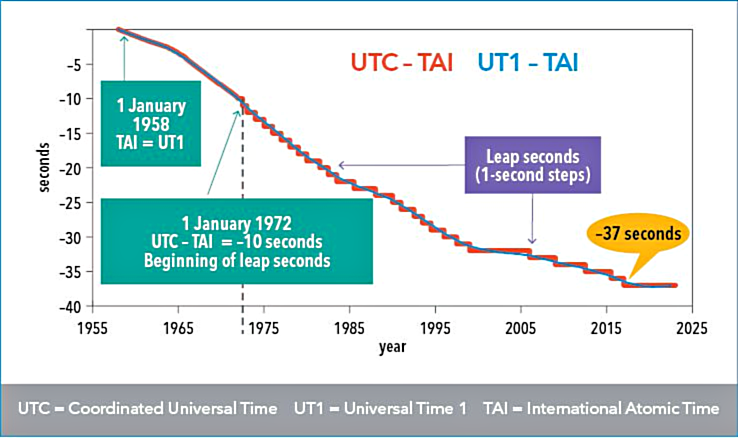
\includegraphics[width=0.55\linewidth]{images/grechnev2.png}
		\caption{Разница между $UT$ и $UTC$}
		\label{grechnev2}
	\end{figure}

	Разница между $UT$/$UTC$ и $TAI$ составляет, на данный момент, $37$ секунд, что иногда может быть очень существенно. И хоть $TAI$ используется довольно редко, предпочтительнее использовать при анализе одномерных временных рядов зависимость величины не от номера отсчета, а от временной отметки, когда данные были получены. Это поможет избежать ошибок из-за:
	\begin{enumerate}
		\item неравномерных отсчетов
		\item записей с пропусками
		\item сбоев записи времени
		\item использования данных с разными шкалами времени
	\end{enumerate}
	В IDL это можно реализовать путем использования команды:
	\begin{python}
		plot, x, y
	\end{python}
	Или при использовании нескольких графиков с разными шкалами:
	\begin{python}
		plot, time1, y1
		oplot, time2, y2
	\end{python}
	В Python для этого можно использовать:
	\begin{python}
		import matplotlib.pyplot as plt
		def format_seconds(x, pos):
		hours = int(x // 3600)
		minutes = int((x % 3600) // 60)
		seconds = int(x % 60)
		return f"{hours:02d}:
		{minutes:02d}:
		{seconds:02d}"
		plt.plot(time, data)
		ax.xaxis.set_major_formatter(
		FuncFormatter(format_seconds))
	\end{python}

	\begin{figure}[h!]
		\centering
		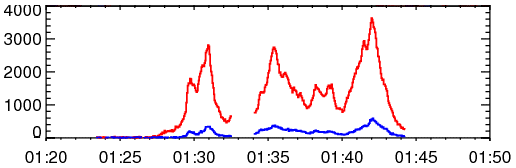
\includegraphics[width=0.65\linewidth]{images/grechnev3.png}
		\caption{Пример правильного отображения данных с пропусками}
		\label{grechnev3}
	\end{figure}

	Подобный подход позволит создать интерактивную ось времени, при манипуляции с которой (приближении и т. п.) метки останутся верными

	Также стоит обратить внимание на валидацию данных и их фильтрацию. К типичным методам можно отнести:
	\begin{enumerate}
		\item сглаживание скользящим усреднением: $[1, 4, 100] \Rightarrow 35$
		\item медианное сглаживание: $[1, 4, 100] \Rightarrow 4$\\
		(может быть полезно для оценки стационарного уровня при анализе всплеска излучения)
		\item суммирование отсчетов\\
		(данный подход нужно использовать с осторожностью из-за его фазочувствительности)
		\item Фурье-фильтрация\\
		(разложение исходного сигнала на гармонические составляющие для выделения шумов)
		\item полиномиальная аппроксимация\\
		(повышение порядка полинома повышает точность, но снижает устойчивость)
		\item выделение огибающих и трендов (см. \cref{grechnev4})\\
		(иногда можно заменить аппроксимацией точек минимумов в массиве данных каким-либо способом)
	\end{enumerate}

	\begin{figure}[h!]
		\centering
		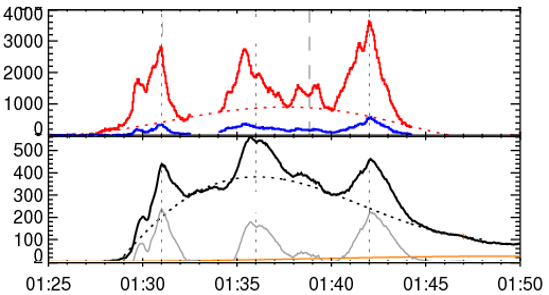
\includegraphics[width=0.65\linewidth]{images/grechnev4.png}
		\caption{Пример использования огибающих}
		\label{grechnev4}
	\end{figure}


	\item \textbf{Двумерные массивы данных (обычно, изображения)}

	\begin{enumerate}
		\item \textsf{Отображение}

		При отображении данных важно правильно подобрать шкалу яркости. Она может быть линейной, степенной, логарифмической, определена какой-то сложной функцией (например, $asinh$), или вообще иметь разные масштабы изменения для разных диапазонов значений (пример -\\ \texttt{matplotlib.colors.TwoSlopeNorm(vcenter, vmin=None, vmax=None)}, что может быть полезно при анализе изображений солнечных вспышек с большим динамическим диапазоном)

		\begin{figure}[h!]
			\centering
			\includegraphics[width=0.75\linewidth]{images/grechnev5.png}
			\caption{Пример использования различных шкал яркости. Для случая линейной шкалы выполнено ограничение по порогу}
			\label{grechnev5}
		\end{figure}

		\begin{figure}[h!]
			\centering
			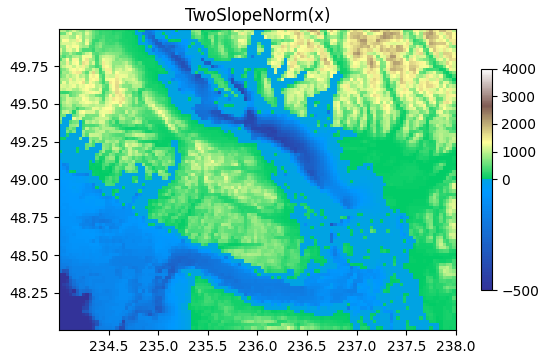
\includegraphics[width=0.7\linewidth]{images/grechnev6.png}
			\caption{Наглядная демонстрация принципа работы нормировки \texttt{TwoSlopeNorm}}
			\label{grechnev6}
		\end{figure}

		Также довольно удобным инструментом анализа изображений являются контуры уровня (см. \cref{grechnev7})

		\begin{figure}[h!]
			\centering
			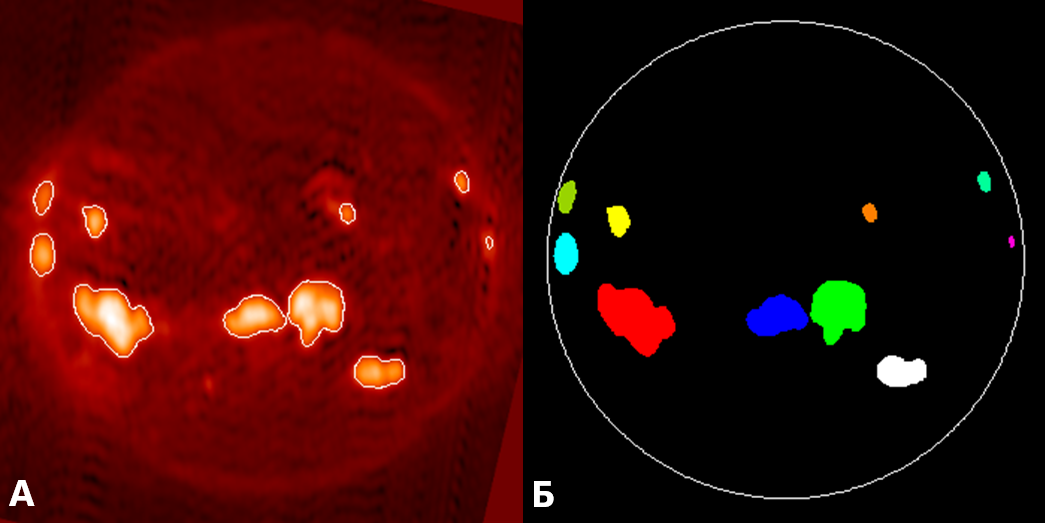
\includegraphics[width=0.7\linewidth]{images/grechnev7.png}
			\caption{А - использование контуров при анализе изображений, Б - "<Раскраска пятен">}
			\label{grechnev7}
		\end{figure}

		\item \textsf{Подавление фона и выделение изменений}

		Для этой цели широко используется разностные изображения. Их есть два вида: бегущие (последовательные) разности (\textit{Running Difference} - RD) и фиксированные разности (\textit{Fixed Difference} - \textit{FD})

		\begin{figure}[h!]
			\centering
			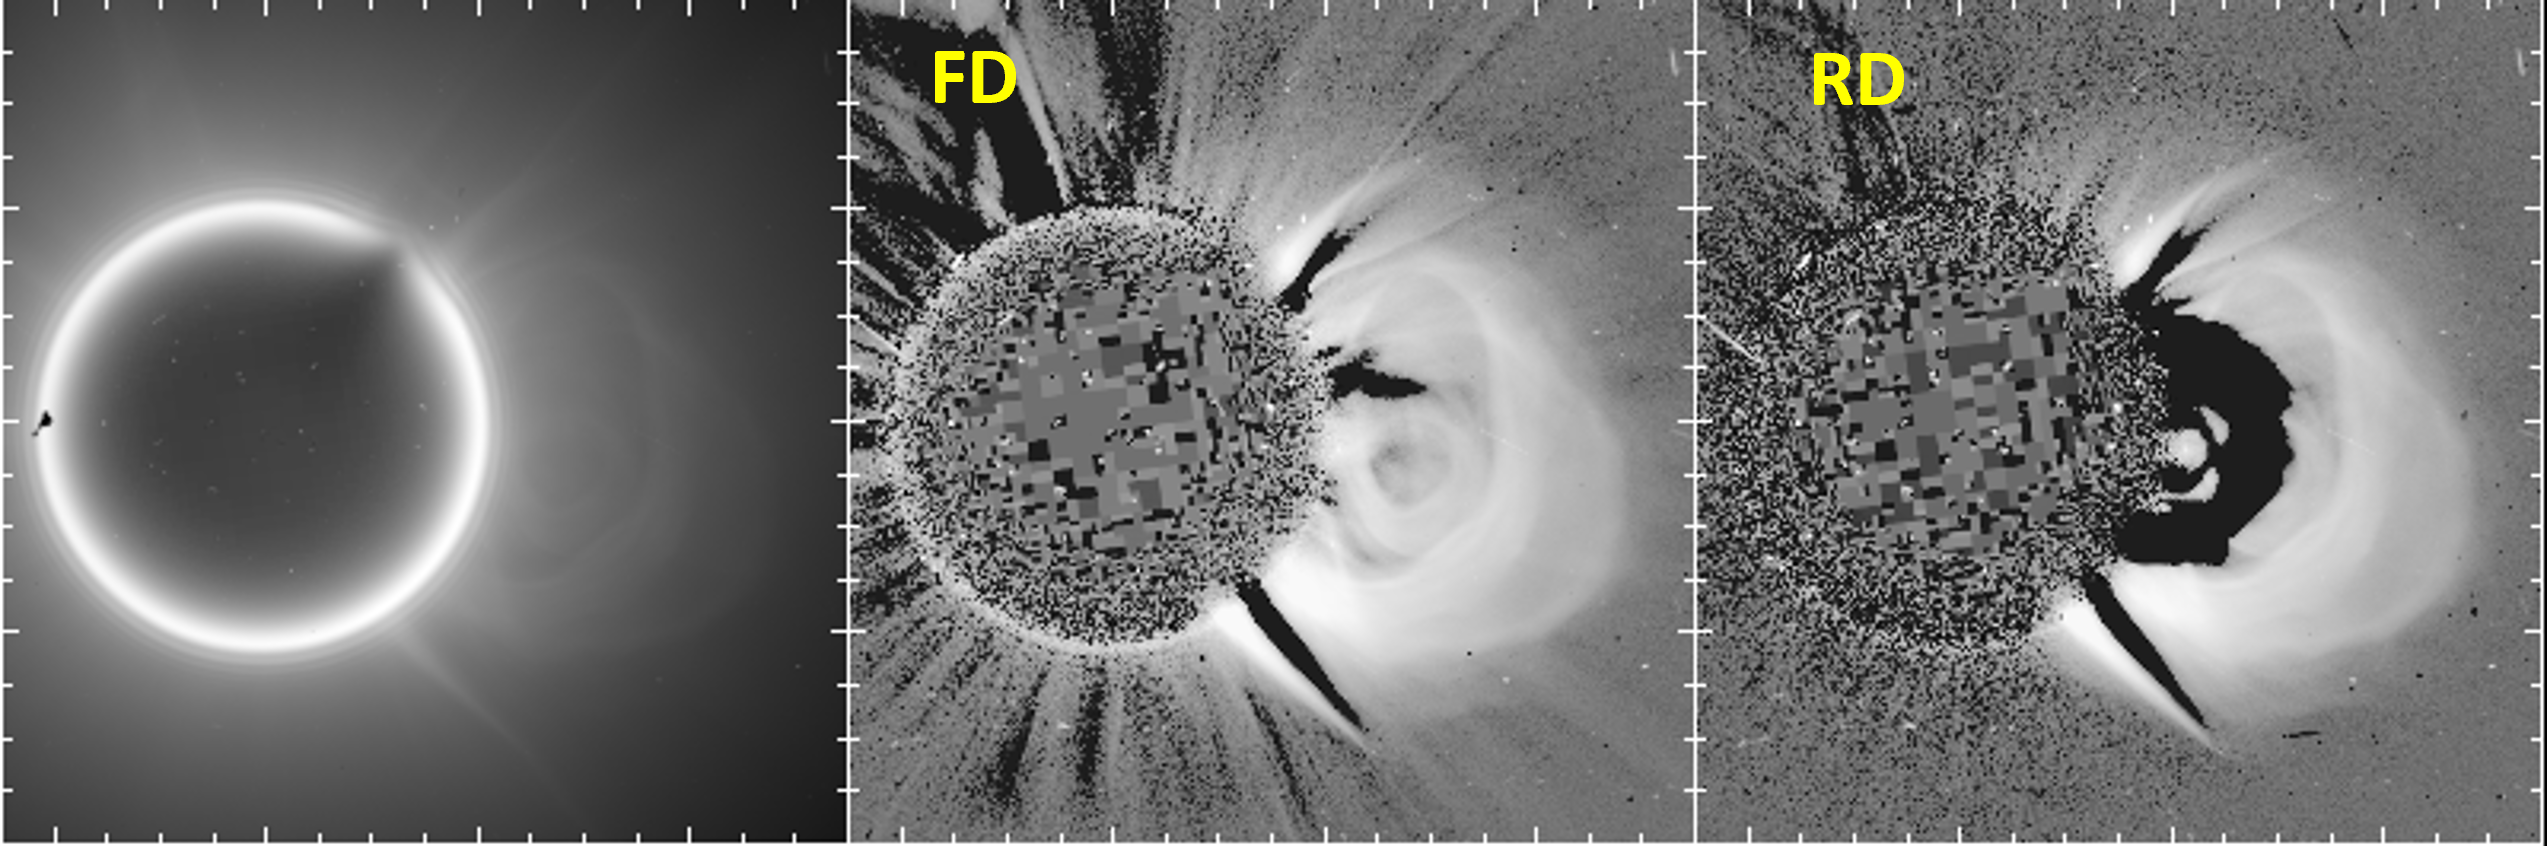
\includegraphics[width=0.7\linewidth]{images/grechnev8.png}
			\caption{Использование разностных изображений. Видно потемнение области }
			\label{grechnev8}
		\end{figure}

	\end{enumerate}
\end{enumerate}




\section{Введение}

\begin{figure}[H]
	\centering
	
\includegraphics[scale=0.55]{img/smile.png}
	\caption{гыгыгыгыгыгыгыгыгы}
	\label{fig:gygygy}
\end{figure}

Это шаблон учебного пособия, в котором можно показывать рисунки (см. рис. \ref{fig:gygygy})

\subsection{Делать подразделы}
Вот

\paragraph{Еще и параграфы}
И ссылаться на литературу \cite{priest}


%!TEX root = ../lectionsA4.tex

\epigraph{\textit{"<Ежели спросят у Вас: что важнее – Солнце или Луна, ответствуйте – Луна. Ибо Солнце светит днем, когда и без того светло, а Луна – ночью">} \\ Козьма Прутков}

\section{Виды и значение калибровок для апертурного синтеза}
Калибровка - одна из самых значимых составляющих наблюдений на радиоинтерферометрах, потому что без них не удастся построить изображение. По данным, не включающим калибровки, можно оценивать лишь некоторые интегральные параметры излучения, например, получить корреляционные кривые, но даже для их правильной интерпретации также необходимо проведение калибровок.

\subsection{Виды калибровок}
Калибровки бывают аппаратные (до наблюдений) и применительно к данным. Аппаратные калибровки чрезвычайно важны, так как после проведения наблюдений нейтрализовать их негативное воздействие практически невозможно\\

\begin{list}{-}{\textbf{Аппаратные}}
	\item \textit{Наведение антенн} \\
	Так как диаграмма направленности антенны с круглой апертурой является функцией Бесселя, и данная функция имеет один выраженный максимум, то он должен смотреть точно на центр солнечного диска. При ошибке наведения возникает наклон (см. рис. \ref{fig:искажения при наведении}), который приводит к неправильной фокусировке облучателя и довольно сложным искажениям как фазы, так и амплитуды. Поэтому необходимо следить за точностью движения моторов и их способностью выдерживать определенные эфимериды, а также за положением облучателя антенны
	\begin{figure}[H]
		\centering
		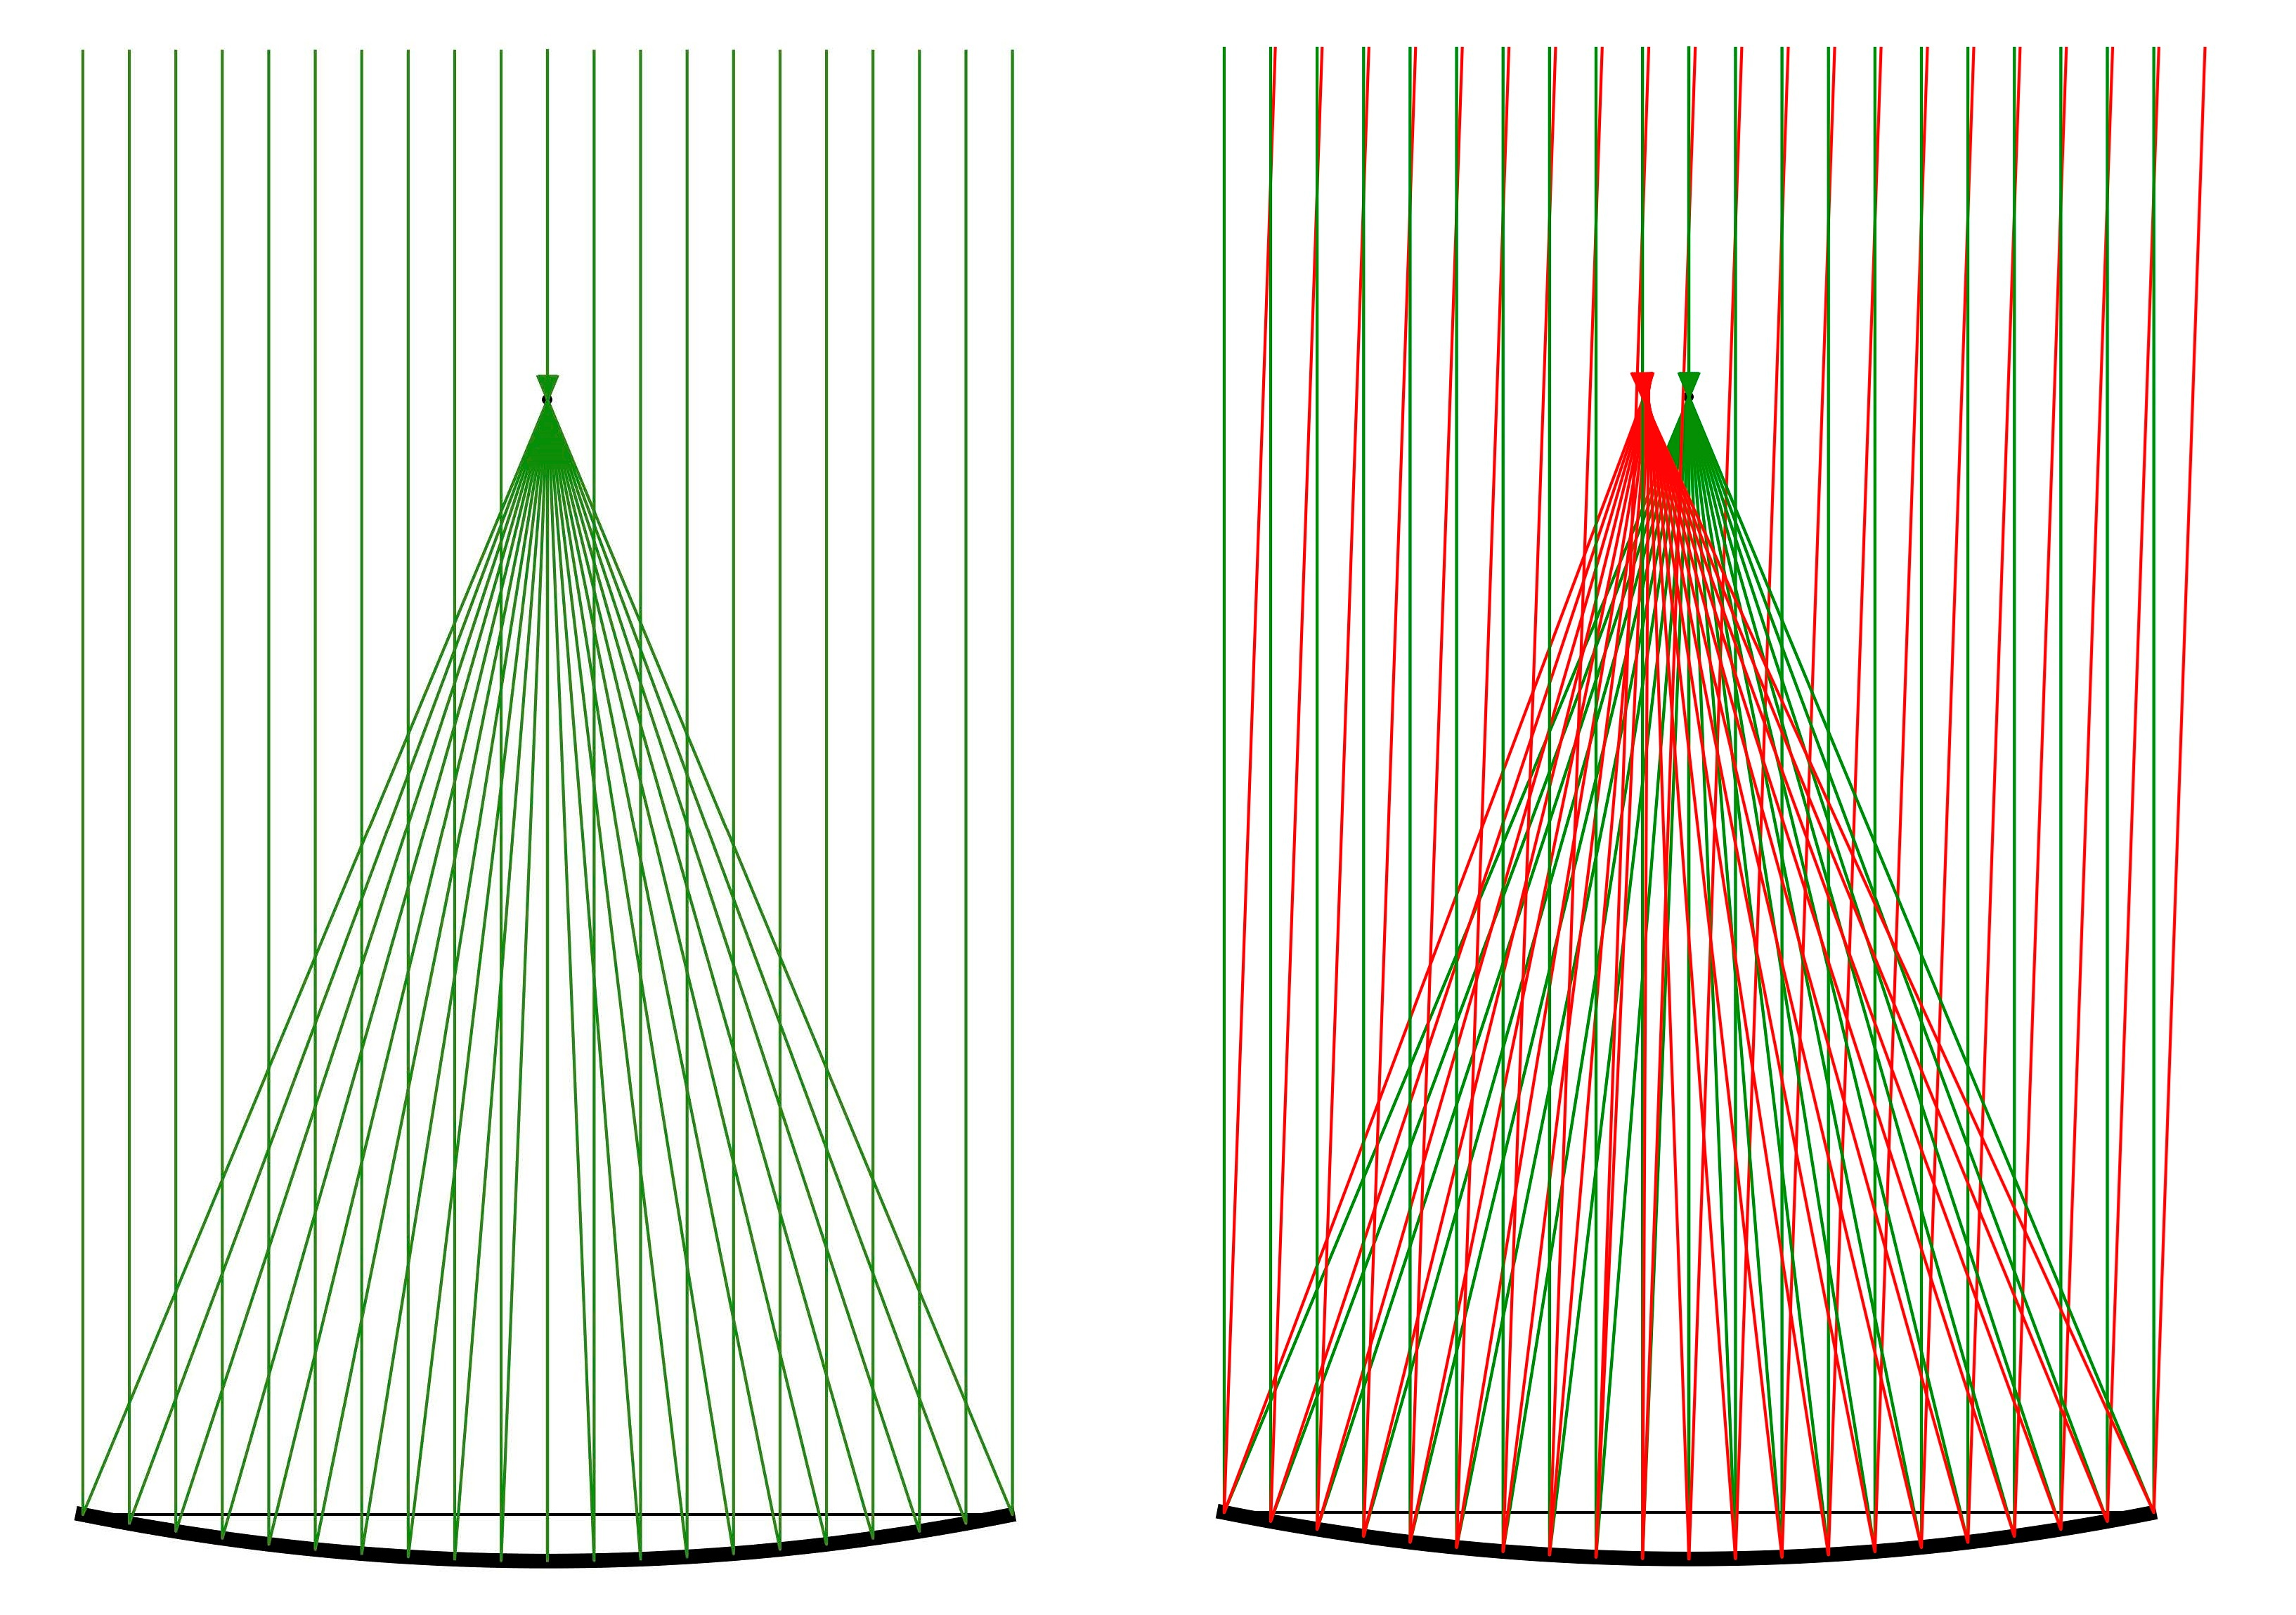
\includegraphics[scale=0.15]{images/globa2.jpg}
		\caption{Ошибки фокусировки при неправильном наведении}
		\label{fig:искажения при наведении}
	\end{figure}

	\item \textit{Положение антенн относительно друг друга}\\ (можно оценить из данных наблюдений и изменить с помощью подстроечных болтов на стойках)

	\textbf{20-30 мин доделать}

	\item \textit{Длины кабелей и идентичность их физических параметров}\\
	На каждой антенне есть приемный модуль, в котором установлен лазер. Он используется для передачи модулированного сигнала по оптоволокну к коррелятору. Однако, если длины кабелей будут различны, то возникнут дополнительные фазовые искажения. Например, различие длин в 1 см даст 36 градусов фазового набега на частоте 3 ГГц.\\
	Для того чтобы этого не допустить, все кабели имеют одинаковую длину в 800 метров, вне зависимости от положения антенн относительно блока коррелятора, и накручены на так называемые "<компенсационные катушки">. Измеряются длины с ограниченной ($\approx 1$ метр) точностью прибором под названием "<рефлектометр">, при этом происходит измерение именно оптической длины, так как электрическая и геометрическая длины оптических кабелей различаются.\\
	Однако есть возможность уточнить измеренную величину с точностью до нескольких миллиметров путем анализа данных наблюдений и поиска линейных наклонов фаз в полосе частот. Эти небольшие отклонения легче компенсировать программными задержками\\
	Также необходимо учитывать, что температурные колебания влияют на абсолютные значения коэффициентов преломления ядра и оптической оболочки оптоволокна, а следовательно, может меняться скорость света внутри кабеля. Для нейтрализации этого эффекта все коммуникации проложены в подземном тоннеле, где круглогодично поддерживается примерно одинаковая температура.

	\item \textit{Точные координаты, временная привязка, стандарт частоты}\\
	Данные величины необходимо знать с максимально возможной точностью для введения задержек в сигнал с целью фазовых корректировок и остановки вращения интерференционных лепестков (возникает из-за относительного движения источника относительно интерферометра, вызванного вращением Земли). \\
	Скорость вращения лепестков пропорциональна $2\pi \nu_{LO} \tau_g$, где $\nu_{LO}$ - частота гетеродина, $\tau_g = ({D}/{c}) * sin \theta$ - геометрическая задержка (рис. \ref{fig:геометрия интерферометра}).
	\begin{figure}[H]
		\centering
		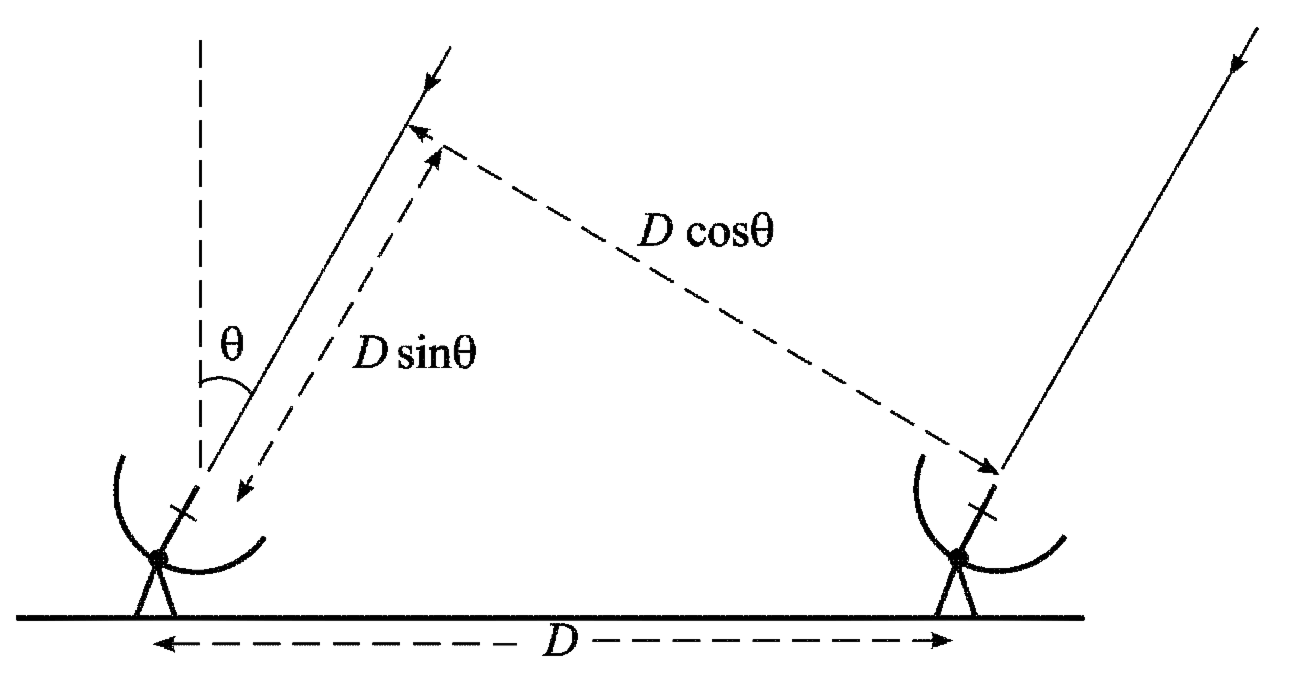
\includegraphics[scale=0.5]{images/geominterferometr.png}
		\caption{Геометрия простого интерферометра. $D$ — база интерферометра}
		\label{fig:геометрия интерферометра}
	\end{figure}

\end{list}

\begin{list}{-}{\textbf{Калибровка данных}}
	\item \textit{Комплексные коэффициенты передачи антенн (antenna-based)}\\
	Под калибровкой данных подразумевается вычисление коэффициентов передачи антенн с использованием данных наблюдений.\\\\
	Методы калибровок данных:
	\begin{itemize}
		\item По наблюдениям точечных источников и известным потоком в полосе частот наблюдений вблизи интересующего объекта (используется преимущественно на звездных радиоинтерферометрах)
		\item С использованием избыточности антенной решетки (много одинаковых пар антенн, измеряющих один и тот же сигнал)
		\item Самокалибровка
	\end{itemize}

	\item ошибки видностей (baseline-based)
\end{list}

\subsection{Самокалибровка}
Самокалибровка производится по наблюдаемому источнику и подразумевает наличие модельного распределения яркости $\hat{I}$, из которого вычисляются модельные видности для каждой пары антенн.

Изначально метод был разработан для того случая, когда общая калибровка проходит по известному объекту, однако он находится в стороне от объекта наблюдения, и при перенаведении телескопа несколько меняется фаза принимаемого сигнала (применять калибровку на одни координаты к другим - в общем случае нельзя). Самокалибровка позволяет вычислить небольшие отклонения и поправки из-за этой смены координат.

Данный метод позволяет получить радиоизображение высокого качества, с динамическим диапазоном порядка $>1000$. Однако для применения самокалибровки необходимо иметь хорошую модель источника, и получить ее -- задача довольно сложная, особенно если учесть высокое разрешение СРГ и необходимость высокой детализации этой модели.

Комплексные коэффициенты передачи антенн при самокалибровке вычисляются путем минимизации функции:
\begin{equation}\label{eq:самокалибровка}
	S = \sum_{k}^{} \sum_{i,j (i \not= j)}^{} \omega_{ij}(t_{k}) \lvert \widetilde{V}_{ij}(t_k) -  g_i(t_k)g_j^*(t_k)\hat{V}_{ij}(t_k) \rvert^2
\end{equation}
где $ \omega_{ij}$ - весовой коэффициент для видности, измеряемой парой антенн $i$ и $j$.\\

Уточнение модели происходит итеративно. Шаги на одной итерации:
\begin{enumerate}
	\item Подобрать модель распределения яркости на небе
	\item Вычислить модельные видности и, подставив их в выражение (\ref{eq:самокалибровка}), найти коэффициенты передачи антенн
	\item Скорректировать измеренные видности на коэффициенты передачи и построить изображения, используя какой-либо метод чистки
	\item Использовать компоненты модели, получаемой при чистке, в качестве нового модельного распределения яркости.
	\item Если результат неудовлетворителен, вернуться к шагу 2.
\end{enumerate}

Метод хорошо применяется к точечным источникам, так как их модельные видности хорошо известны.

\subsection{Калибровка по избыточности}
Данный метод возможно использовать, не зная об источнике абсолютно ничего. Единственное условие применимости данного метода - SNR (отношение сигнал/шум) для каждой видности должно быть $5$ или более. Решение можно найти с точностью до линейного наклона фаз и константы по амплитуде, что
приводит к произвольному положению Солнца в кадре и произвольной яркостной температуре. Эти
эффекты корректируются дополнительными методами.

\begin{figure}[H]
	\centering
	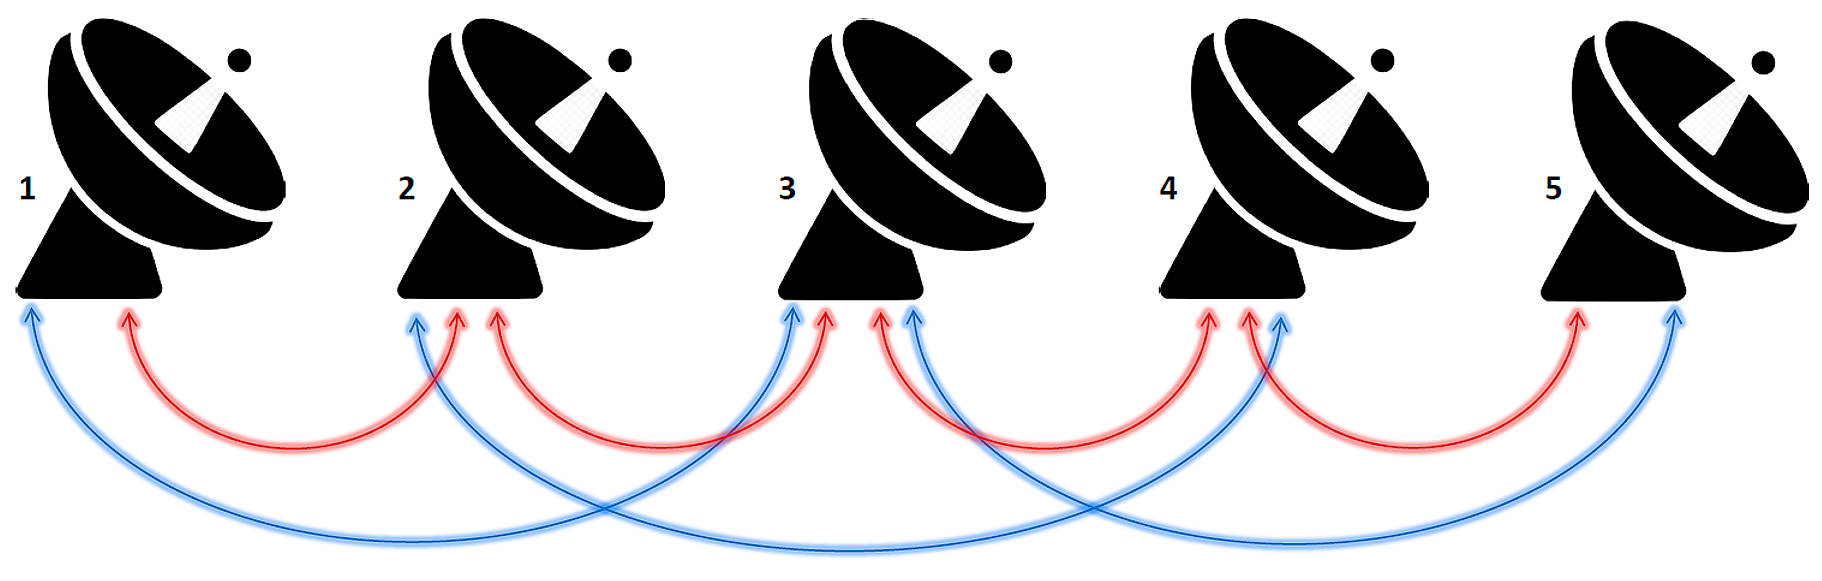
\includegraphics[scale=0.35]{images/calibrate_cheme.png}
	\caption{Схема составления пар антенн для калибровки по избыточности}
	\label{fig:калибровка по избыточности}
\end{figure}

Для построения изображения используются перекрестные базы, а для калибровки - избыточные базы между антеннами одного луча. Если при калибровке использовать только короткие базы, этого будет достаточно для фазовой калибровки, но недостаточно для амплитудной, так как это приводит к появлению артефактов (см. рис. \ref{fig:temp_calib}) -- поэтому необходимо использовать также и длинные избыточные базы.

Итак, нам необходимо решить систему уравнений вида
\begin{equation}\label{eq:калибровка по избыточности 1}
	\widetilde{V}_{kl} = g_kg_l^*V_{kl}
\end{equation}
Как можно заметить из рис. \ref{fig:калибровка по избыточности}, видности на некоторых парах антенн у нас повторяются, а именно:\\
\begin{equation}\label{eq:повторы баз 1}
	V_1 = V_{13} = V_{24} = V_{35}
\end{equation}
\begin{equation}\label{eq:повторы баз 2}
	V_2 = V_{12} = V_{23} = V_{34} = V_{45}
\end{equation}

Аналитически эту систему уравнений решить невозможно, так как все величины комплексные, а уравнения нелинейные. Так как линеаризация этой системы также довольно сложна, решается система численно методами нелинейной минимизации.

Однако покажем, как можно линеаризовать эту систему методом взятия логарифма. \\
Представим ${V}_{kl}(t)$ и ${g}_{k}(t)$ как комплексные числа, перенеся амплитуды под экспоненту:
\begin{equation}\label{eq:замена видности}
	{V}_{kl}(t) = \exp({S}_{kl} + i\psi_{kl}(t))
\end{equation}
\begin{equation}\label{eq:замена коэф передачи}
	{g}_{k}(t) = \exp({a}_{k} + i\phi_{k}(t))
\end{equation}
Подставим замену в изначальное уравнение (\ref{eq:калибровка по избыточности 1}) и возьмем от получившегося выражения логарифм:
\begin{equation}\label{eq:подстановка в 1.2}
	\tilde{S}_{kl}(t) + i\tilde{\psi}_{kl}(t) = {a}_{k}(t) + {a}_{l}(t) + {S}_{kl}(t) + i (\phi_{k}(t) + \phi_{l}(t) + {\psi}_{kl}(t))
\end{equation}
Можно разделить уравнения для фаз и амплитуд:
\begin{equation}\label{eq:разделение для амплитуд}
	\tilde{\psi}_{kl}(t) = \phi_{k}(t) + \phi_{l}(t) + {\psi}_{kl}(t)
\end{equation}
\begin{equation}\label{eq:разделение для фаз}
	\tilde{S}_{kl}(t) = {a}_{k}(t) + {a}_{l}(t) + {S}_{kl}(t)
\end{equation}

\begin{equation}
	\mqty( % It's require package "physics"
	1&-1&0&0&1\\	0&1&-1&0&1\\	0&0&1&-1&1\\	1&0&0&-1&1
	)
	\mqty(
	\phi_{1}\\	\phi_{2}\\	\phi_{3}\\	\phi_{4}\\	\phi_{5}\\	\psi
	)=
	\mqty(
	\tilde{\psi}_{12}\\	\tilde{\psi}_{23}\\	\tilde{\psi}_{34}\\	\tilde{\psi}_{45}
	)
\end{equation}

Когда система недоопределена, у нее всегда есть вектор, принадлежащий нулевому пространству матрицы. Это вектор, который при умножении матрицы на него дает 0. Если

\begin{equation}
	\mqty(
	\phi_{1}\\	\phi_{2}\\	\phi_{3}\\	\phi_{4}\\	\phi_{5}\\	\psi
	)=
	C_1	\mqty(
	1\\	1\\	1\\	1\\	1\\	0\\
	)+
	C_2	\mqty(
	1\\	2\\	3\\	4\\	5\\	0\\
	)
\end{equation}

Система уравнений недоопределена, поэтому имеет бесконечное множестворешений, отличающихся на вектора нулевого пространства матрицы:

\begin{equation}
	\mqty(
	\phi_{1} - \phi_{2} + \phi = \tilde{\psi}_{12}\\
	\phi_{2} - \phi_{3} + \phi = \tilde{\psi}_{23}\\
	\phi_{3} - \phi_{4} + \phi = \tilde{\psi}_{34}\\
	\phi_{4} - \phi_{5} + \phi = \tilde{\psi}_{45}
	)
\end{equation}

Добавление новых уравнений в систему (для более длинных баз) не меняет вид векторов нулевого пространства

\begin{equation}
	\mqty(
	1&-1&0&0&0&1\\	1&-1&0&0&0&1\\	0&1&-1&0&0&1\\	-1&0&0&1&0&1\\ 0&0&1&-1&0&1\\ 1&0&0&0&-1&1
	)
	\mqty(
	\phi_{1}\\	\phi_{2}\\	\phi_{3}\\	\phi_{4}\\	\phi_{5}\\	\psi_1\\ \psi_2
	)=
	\mqty(
	\tilde{\psi}_{12}\\	\tilde{\psi}_{23}\\	\tilde{\psi}_{34}\\	\tilde{\psi}_{45}\\ \tilde{\psi}_{13}\\ \tilde{\psi}_{24}\\ \tilde{\psi}_{35}
	)
\end{equation}

\begin{equation}
	\mqty(
	\phi_{1}\\	\phi_{2}\\	\phi_{3}\\	\phi_{4}\\	\phi_{5}\\ \psi_1\\ \psi_2\\
	)=
	C_1	\mqty(
	1\\	1\\	1\\	1\\	1\\	0\\ 0\\
	)+
	C_2	\mqty(
	1\\	2\\	3\\	4\\	5\\	1\\ 2\\
	)
\end{equation}

Для калибровки амплитуд нужно использовать как минимум первые и вторые базы.\\
Система уравнений для первых баз:

\begin{equation}
	\mqty( % It's require package "physics"
	1&1&0&0&0&1\\	0&1&1&0&0&1\\	0&0&1&1&0&1\\	0&0&0&1&1&1
	)
	\mqty(
	a_{1}\\	a_{2}\\	a_{3}\\	a_{4}\\	a_{5}\\	S
	)=
	\mqty(
	S_{12}\\	S_{23}\\	S_{34}\\	S_{45}
	)
\end{equation}

Из нее можно получить вектор нулевого пространства:
\begin{equation}
	\mqty(
	a_{1}\\	a_{2}\\	a_{3}\\	a_{4}\\	a_{5}\\	S
	)=C_1
	\mqty(
	1\\	1\\	1\\	1\\	1\\ -2\\
	)+C_2
	\mqty(
	-1\\ 1\\ -1\\ 1\\ -1\\  0\\
	)
\end{equation}

Система уравнений для первых и вторых баз:


Нужно помнить также о том, что SNR меняется на базах антенн с течением времени. Если отследить это изменение в течение дня, можно заметить, что в определенные моменты времени SNR приближается к нулю (рис. \ref{fig:SNRonbase}). Происходит это из-за смены проекции баз, что приводит к измерению базой разных пространственных частот.

Также важно помнить, что на решетке 6-12 ГГц нет центральной антенны в перекрестии, что приводит к дополнительной константе по фазе во всём спектре, что в свою очередь ведет к перекосу изображения и смене знака вторичного солнечного диска.

\begin{figure}[H]
	\centering
	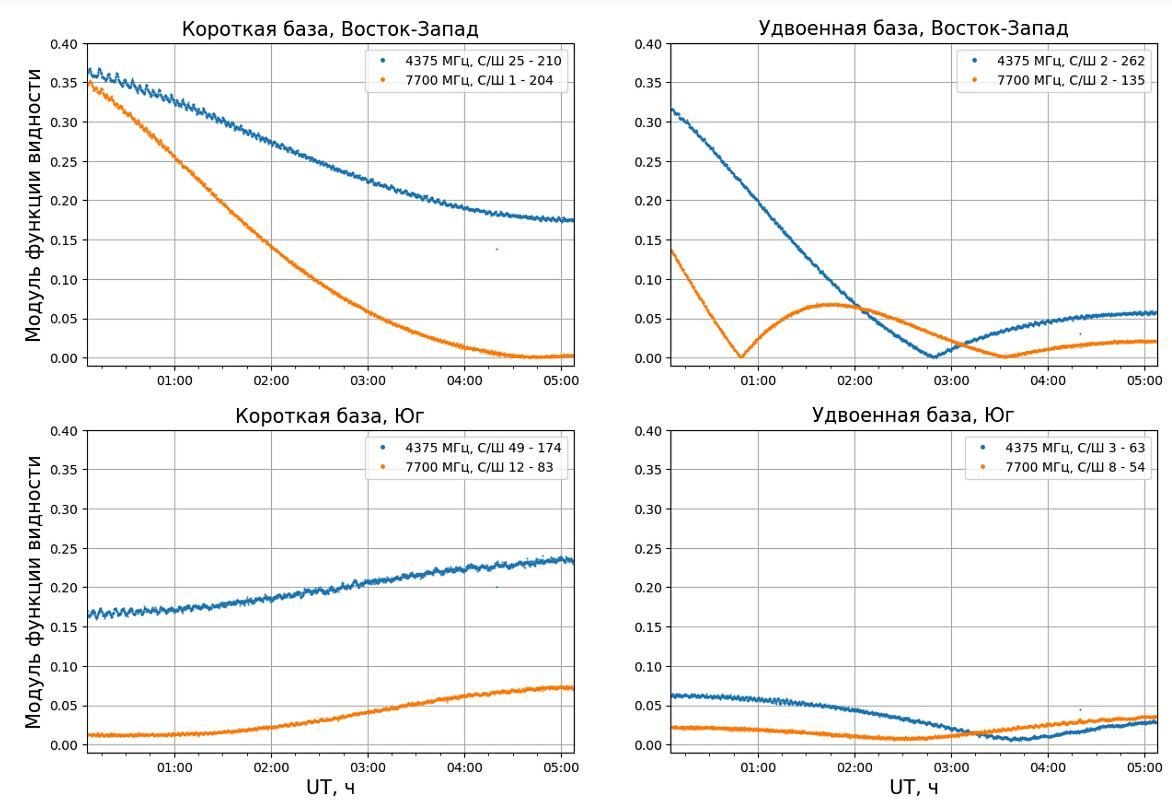
\includegraphics[scale=1]{images/SNRonbase.jpg}
	\caption{Изменение SNR на базах в течение дня}
	\label{fig:SNRonbase}
\end{figure}

На изображениях Солнца отсутствие и наличие фазовой калибровки выглядит, как представлено на рис. \ref{fig:notcalibandcalib}

\begin{figure}[H]
	\centering
	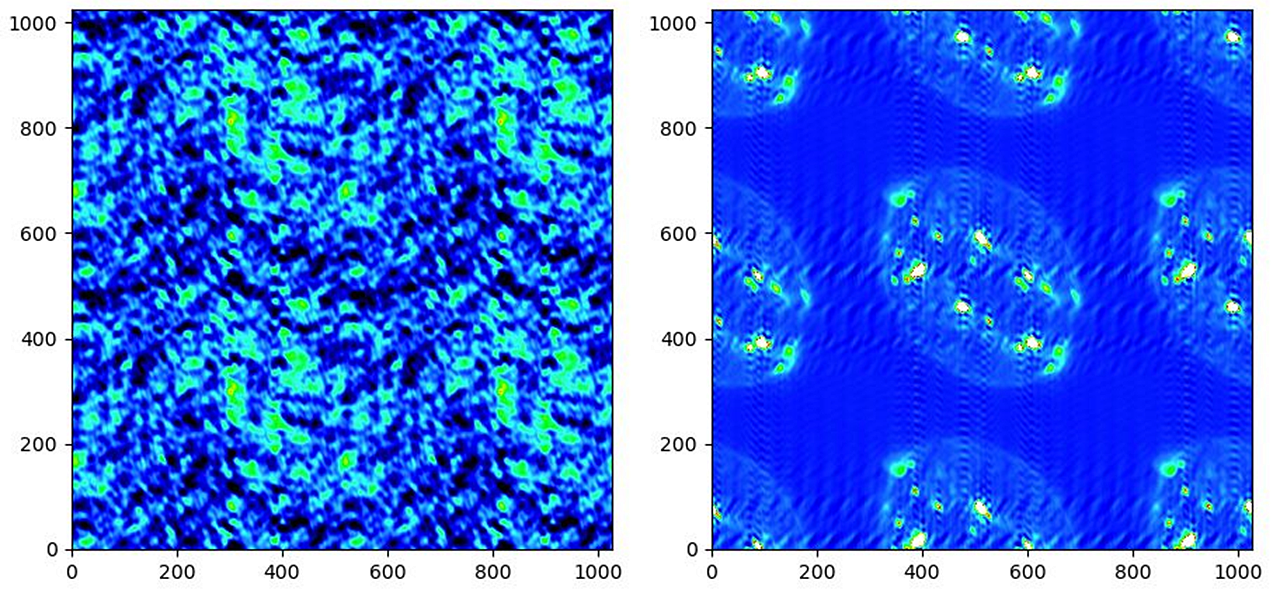
\includegraphics[width=1\linewidth]{images/notcalib_and_calib}
	\caption{Радиоизображение Солнца без фазовой калибровки и при ее наличии}
	\label{fig:notcalibandcalib}
\end{figure}

Также положительное влияние фазовой калибровки хорошо заметно и на $UV$-плоскости (рис. \ref{fig:UV_notcalibandcalib}).

\begin{figure}[H]
	\centering
	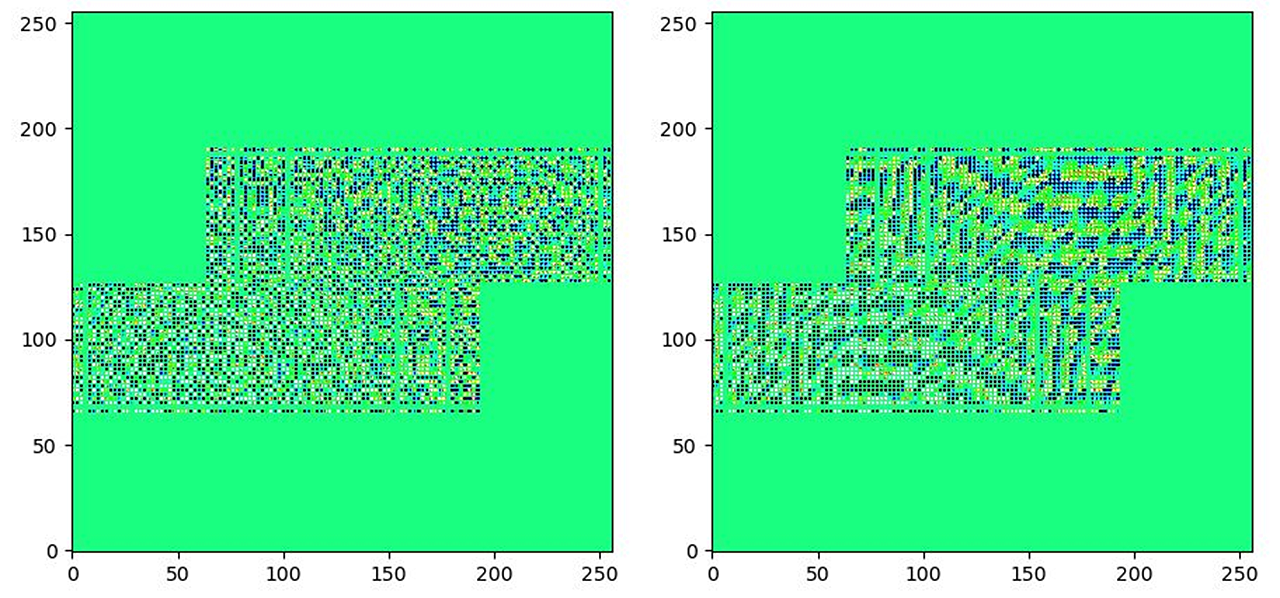
\includegraphics[width=1\linewidth]{images/UV_notcalib_and_calib}
	\caption{Фазовый портрет на $UV$-плоскости без фазовой калибровки и при ее наличии}
	\label{fig:UV_notcalibandcalib}
\end{figure}

\begin{figure}[H]
	\centering
	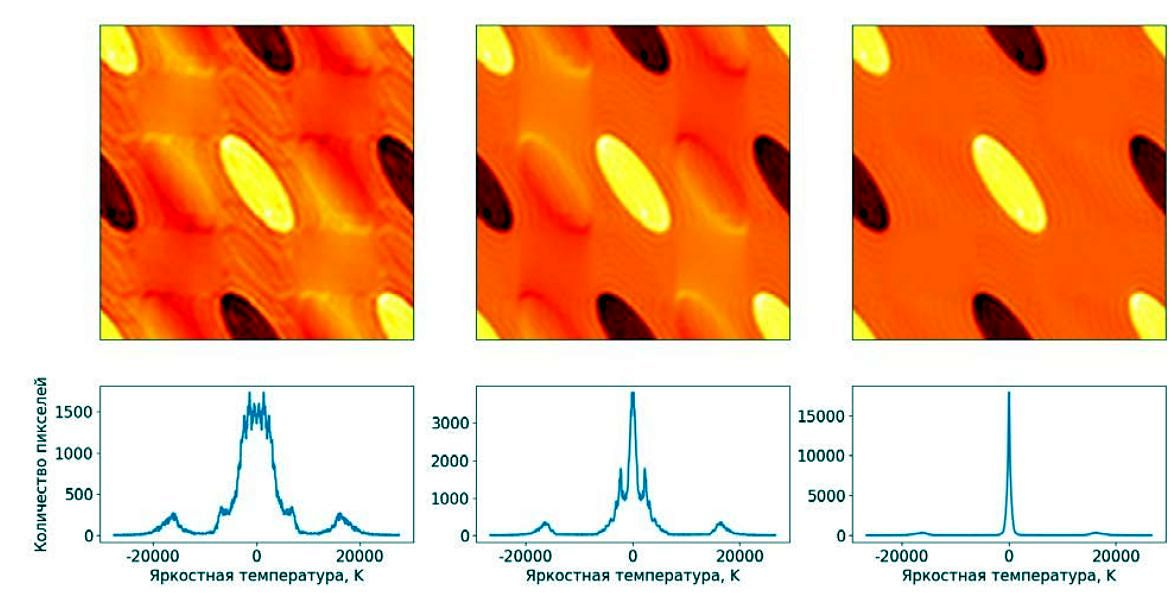
\includegraphics[width=1\linewidth]{images/temp_calib}
	\caption{Влияние амплитудной калибровки на изображения}
	\label{fig:temp_calib}
\end{figure}

На рис. \ref{fig:temp_calib} показано влияние амплитудной калибровки на получающееся изображение. Видно наличие артефактов и размытие гистограммы распределения яркостной температуры на левой (сопутствует калибровке только по коротким базам) и центральной (сопутствует калибровке и по длинным базам) картинках. Правая картинка соответствует хорошей фазовой и амплитудной калибровкам.

\begin{figure}[H]
	\centering
	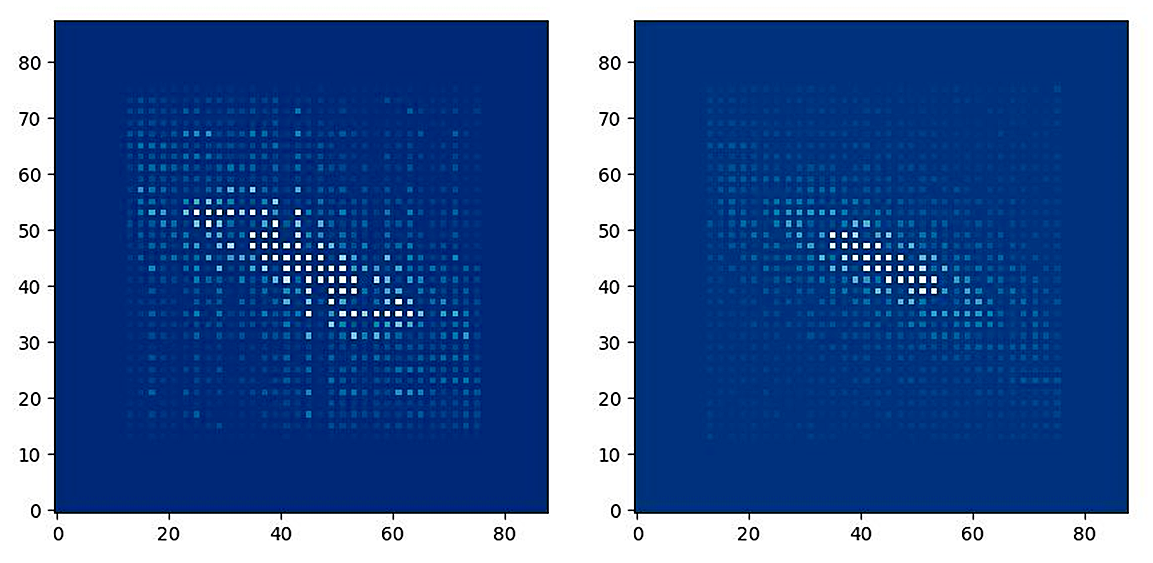
\includegraphics[width=1\linewidth]{images/amplitude_notcalib_and_calib}
	\caption{Влияние амплитудной калибровки на фазовую плоскость}
	\label{fig:amplitude_notcalib_and_calib}
\end{figure}

\noindent\textit{Подробнее о методе калибровки по избыточности можно прочитать в работах \cite{Wieringa}, \cite{Liu}}

\subsection{Корректировка остаточных эффектов}
После проведения калибровки необходимо произвести привязку яркостных температур и выполнить центрирование солнечного диска.

\subsubsection{Привязка температур}
Задача -- для каждой антенны перейти к антенной температуре и потокам. Существует два метода выполнения этой процедуры.

Первый заключается в анализе гистограммы распределения радиояркости на изображении \cite{trees}. Так как большую часть изображения занимает солнечный диск, можно сказать, что максимумом гистограммы является полученная яркостная температура спокойного Солнца. Зная "<эталонную"> температуру на разных частотах, в частности, из работы \cite{Zirin}, можно внести корректировки в изображение, домножив его на некоторый коэффициент и тем самым сместив максимум гистограммы.

Второй метод состоит в абсолютной привязке температур к известной величине.

Пусть на небе существует объект с яркостной температурой $T_B$, сигнал от которого принимает антенна c эффективной площадью $A_{eff}$.\\
Привяжем мощностную характеристику к некоторой $T_A$
\begin{equation}\label{eq:антенная температура}
	T_A = \dfrac{1}{\lambda^2} \int_{4 \pi}^{} A_{eff} T_B (\Omega) d\Omega
\end{equation}
Эту формулу можно оценивать как нормированный отклик антенны, умноженный на некоторую эффективную площадь. В случае, если $T_B$ постоянна для всей замкнутой поверхности вокруг антенны (случай безэховой камеры), то можно вынести ее из под знака интеграла как константу, и антенная температура окажется равной яркостной:
\begin{equation}\label{eq:равность температур}
	T_A = T_B
\end{equation}
Это позволит получать значения в единицах плотности потока ($SFU$):
\begin{equation}\label{eq:перевод в плотность потока}
	S_V = \dfrac{2kT_A}{\lambda^2} \Omega
\end{equation}

Однако для интерферометра нет безэховой камеры, а поток излучения от Солнца постоянно меняется.

Луна -- один из источников, который можно использовать для привязок из-за ее стабильности: поток меняется в пределах $10\%$ в зависимости от ее фазы. Однако до конца не ясно, как должен выглядеть спектр Луны в диапазоне наблюдений СРГ (3-24 ГГц).

Также стоит учитывать уровень сигнала и необходимую для его принятия чувствительность. Яркостная температура Луны -- около $200~K$, антенная температура СРГ при этом составит всего около $20~K$. Кроме того, влияет поглощение в атмосфере (особенно, когда точка наблюдений близка к горизонту) и погода (облачность) - снижение уровня принимаемого излучения может быть сопоставимо или даже превышать $20~K$. Антенная температура же при наблюдениях Солнца -- $1500$-$2000~K$.

\begin{figure}[H]
	\centering
	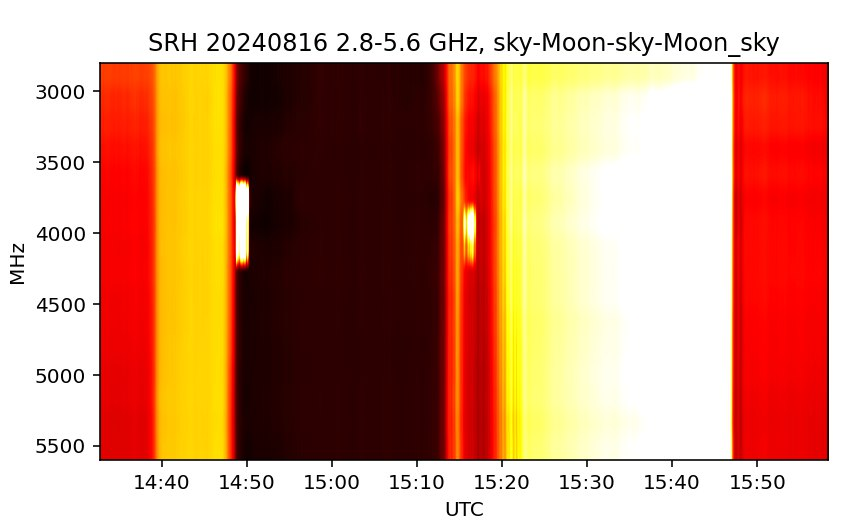
\includegraphics[width=0.7\linewidth]{images/moon_spectre}
	\caption{Спектрограмма наблюдений Луны с перерывами на наблюдения неба}
	\label{fig:moon_spectre}
\end{figure}

\begin{figure}[H]
	\centering
	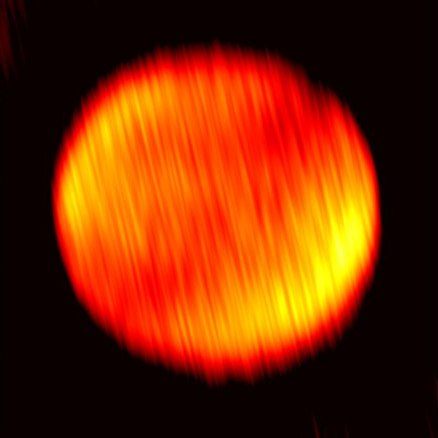
\includegraphics[width=0.7\linewidth]{images/moon_radio}
	\caption{Изображение Луны в радиодиапазоне, сумма нескольких частот, макс. 4.8 ГГц}
	\label{fig:moon_radio}
\end{figure}

На некоторых радиотелескопах для этих целей используется искусственная Луна (например, на Карадагском полигоне в Крыму) - большой черный диск на некотором расстоянии от интерферометра.\\ На СРГ для калибровки используется лес, постольку поскольку он, во первых, является довольно стабильным источником, а во вторых, с помощью него можно создать некий эквивалент безэховой камеры. Это осуществимо потому, что главный лепесток антенн можно полностью закрыть этим лесом. Зная ширину диаграммы направленности, температуру леса, которая примерно равна температуре окружающей среды и частоту наблюдений также можно рассчитать и внести соответствующие корректировки.\\
Каждая сессия ежедневных наблюдений оканчивается наведением антенн на лесной массив вблизи обсерватории.

Таким образом, алгоритм привязки яркостной температуры на данный момент таков: ежедневно подбирается такая зависимость оптической толщины леса в диапазоне частот наблюдений СРГ, чтобы  калибровка по потокам совпала с данными Нобеямского спектрополяриметра -- пока проводится подгонка для разных времен года.

В данный момент рассматривается идея с экранированием облучателя антенны радиопоглощающим материалом, с целью определения оптической толщины леса.

\subsubsection{Привязка координат}
Существуют различные алгоритмы поиска окружностей на изображении, однако здесь невозможно их использовать из-за наложений вторичных солнечных дисков.

В пакете \texttt{srhdata} для центрирования диска строится модельный диск Солнца, который затем сворачивается с диаграммой направленности интерферометра, и уже полученная функция соотносится с результатом наблюдений, который и подгоняется под модель.

Возможно выполнять выравнивание, опираясь на данные наблюдений в других диапазонах, используя пятна и стабильные микроволновые источники над ними. Данный метод позволяет соотнести изображения более точно, но также имеет свои недочеты, в частности, пятенные источники обычно пропадают на частотах 13-15 ГГц, и выше этих значений уже не наблюдаются.


\subsection{Как калибровать?}
Математически задачу калибровки можно описать так. Пусть у нас есть некоторое выражение
\begin{equation}\label{eq:видности}
	\widetilde{V}_{kl}(t) = g_k(t)g_l^*(t)G_{kl}(t)V_{kl}(t) + \epsilon_{kl}(t) + \varepsilon_{kl}(t)
\end{equation}
где:
\begin{list}{-}{}
	\item $\widetilde{V}_{kl}(t)$ -- измеренная видность
	\item  $V_{kl}$ -- истинная видность, то есть компонента пространственного спектра функции, из которой мы можем построить изображение (иначе говоря, Фурье-компонента пространственного спектра распределения яркости, соответствующая базе).
\end{list}
Остальные параметры выражения имеют аппаратное происхождение, а именно:
\begin{list}{-}{}
	\item $g_k(t)$ и $g_l^*(t)$ -- коэффициенты передачи $k$-ой и $l$-ой антенны ($l$ - сопряженная антенна)
	\item $\varepsilon_{kl}(t)$ -- температурные шумы
	\item $G_{kl}(t)$ -- ошибки, связанные с конкретной базой
	\item $\epsilon_{kl}(t)$ -- аддитивная постоянная составляющая для пары антенн (например, ошибки коррелятора - подобное можно отследить)
\end{list}

От ошибок $G_{kl}(t)$ и $\varepsilon_{kl}(t)$ стараются всегда избавиться инструментально. Получать эти ошибки из системы уравнений - очень трудоёмкая задача, т.к. их нельзя разложить на отдельные множители, связанные с антеннами.

Таким образом, суть калибровки можно свести к определению истинных видностей $V_{kl}(t)$ путем поиска и учета паразитных членов в правой части выражения \eqref{eq:видности}.

Радиотелескопы апертурного синтеза в общем случае нельзя скалибровать раз и навсегда из-за:
\begin{itemize}
	\item недостаточной точности позиционирования антенн (возникают	дополнительные набеги фаз, зависящие от координат источника на небесной сфере)
	\item не идентичной конструкции антенн (плохое наведение отдельных антенн, их различные передаточные характеристики)
	\item влияния температуры и характеристик окружающей среды на параметры приемного тракта антенны
	\item влияния атмосферы (дополнительный набег фаз из-за разной толщи атмосферы, через которую проходит излучение)
\end{itemize}

\subsection{Пространственные гармоники}
Каждая пара антенн измеряет свою пространственную гармонику, которая в свою очередь является очень сложной функцией переменной частоты (зависит от проекции базы) и опирается значение функции Бесселя (диаграмма направленности одиночной антенны). Пространственные гармоники в пределах малых углов можно интерпретировать как идеальные двумерные гармоники и использовать для их расчета обычный Фурье-анализ.

При этом пространственная частота и ориентация гармоники определяются вектором базы и частотой приема (см. короткую "<низкочастотную"> и длинную "<высокочастотную"> базы на рис. \ref{fig:гармоники}): чем больше база, тем выше частота и тем менее протяженные объекты можно обнаружить.

\begin{figure}[H]
	\centering
	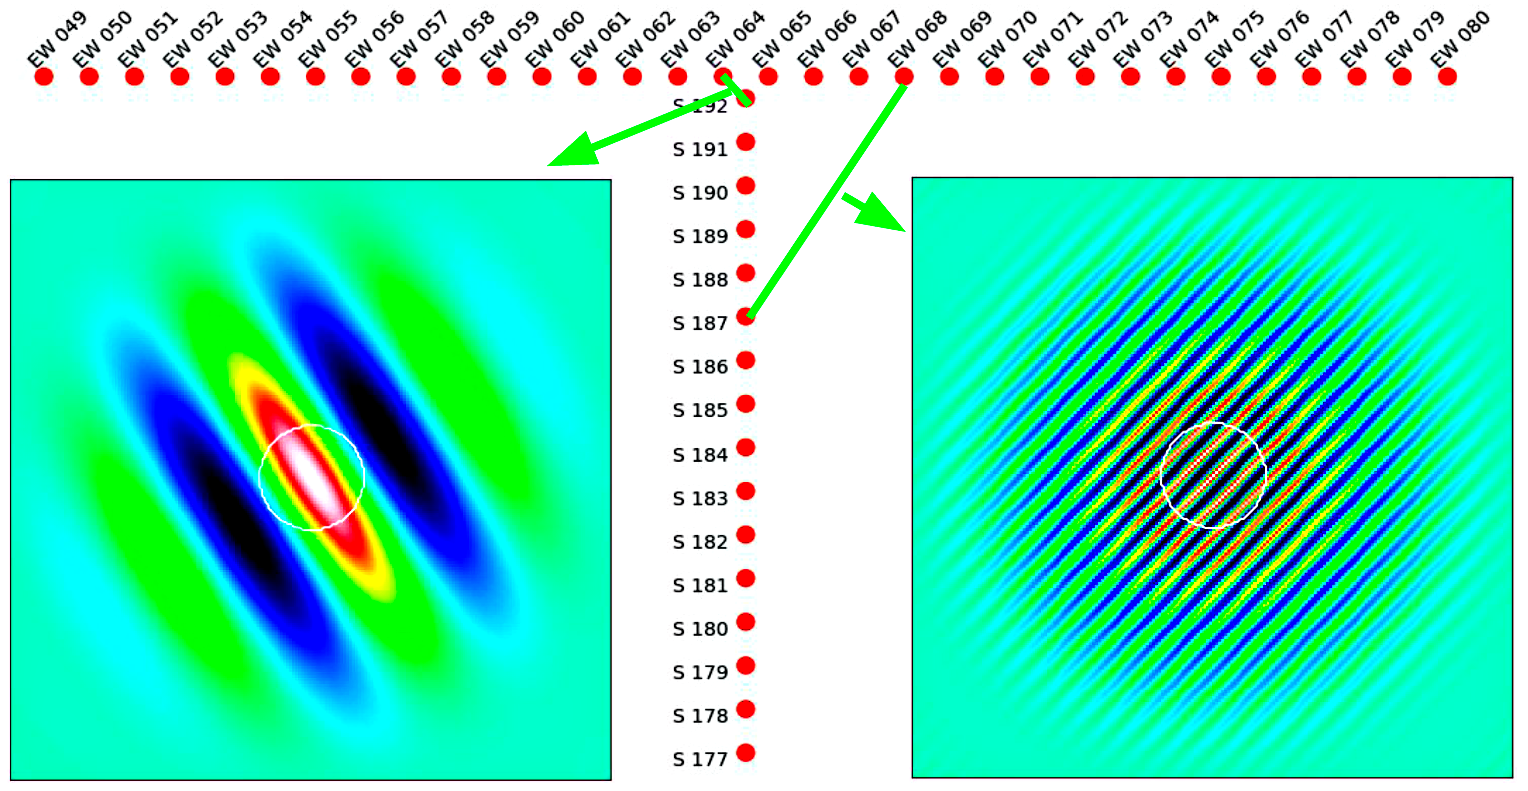
\includegraphics[scale=0.43]{images/globa1.png}
	\caption{Измерение парами антенн пространственных гармоник}
	\label{fig:гармоники}
\end{figure}

$UV$-плоскость формируется путем комбинирования результатов измерений пространственных гармоник каждой антенной пары. $UV$-плоскость позволяет визуализировать пространственную информацию о наблюдаемом объекте с высоким разрешением. Обработка данных в $UV$-плоскости обеспечивает возможность нахождения деталей и структур объектов, а также их спектральных характеристик.

\section{Построение изображений Сибирского Радиогелиографа}
\subsection{Заполнение $UV$-плоскости}
СРГ представляет собой комплекс из трех антенных решеток:
\begin{itemize}
	\item 3-6 ГГЦ: 129 антенн диаметром 3 метра с эквидистантной расстановкой в 9.8 метра, восточный, западный и северный лучи -- первый длиннее остальных, что приводит к несимметричной $UV$-плоскости
	\item 6-12 ГГЦ: 192 антенн диаметром 2 метра с эквидистантной расстановкой в 4.9 метра, каждый луч имеет 64 антенны, но нет связующей антенны между лучами
	\item 12-24 ГГЦ: 207 антенн диаметром 1 метр с неэквидистантным расположением -- центральный сектор имеет плотное расположение, далее шаг увеличивается в 2 раза, еще дальше - в 4 раза от первоначальной величины в \textcolor{red}{2.45} метра. Сделано это для увеличения пространственного разрешения
\end{itemize}

\begin{figure}[H]
	\centering
	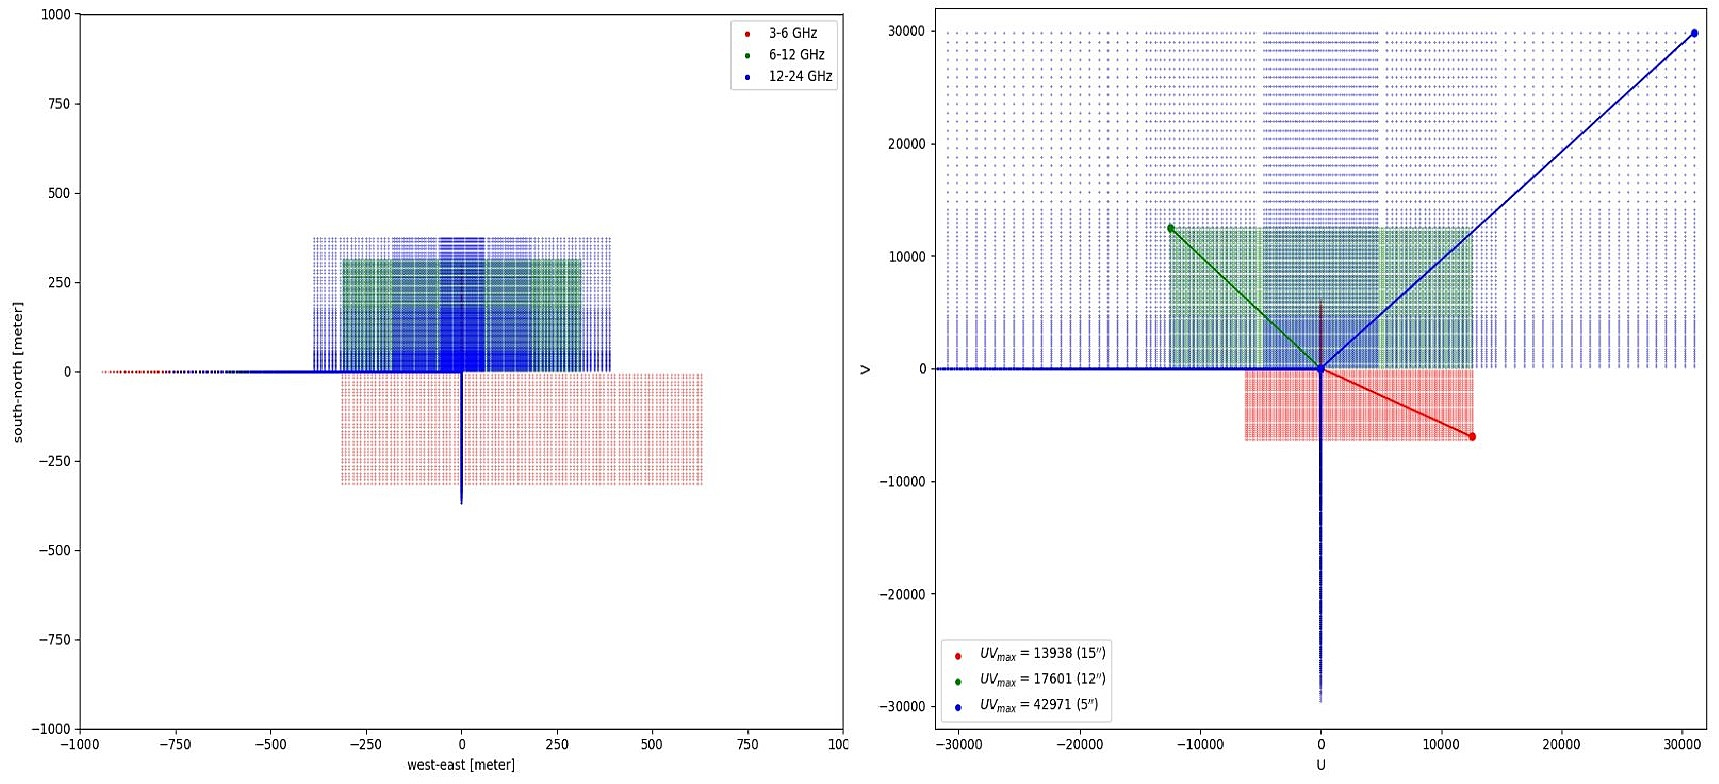
\includegraphics[scale=0.28]{images/srh_UV}
	\caption{Заполнение $UV$-плоскости антеннами различных диапазонов: отображение в метрах (слева) и пространственных частотах (справа). Красным обозначена решетка 3-6 ГГц, зеленым -- 6-12 ГГц, синим -- 12-24 ГГц}
	\label{fig:srh_UV}
\end{figure}

На рис. \ref{fig:srh_UV} представлены $UV$-плоскости для различных антенных решеток СРГ, причем отображены как перекрестные базы, так и избыточные базы, образуемые антеннами на одном луче. Как видно по левой части изображения, где $UV$-плоскость отображена в метрах, на решетке 3-6 ГГц линия с этими избыточными базами выходит наиболее далеко -- это объясняется наибольшей длиной луча этой решетки, равной 900-ам метрам. Также видно и неравномерное покрытие решетки 12-24 ГГц.

Полоски, тянущиеся на \ref{fig:srh_UV}, определяют максимальное пространственное разрешение. Можно увидеть, насколько возможное разрешение решетки 12-24 ГГц превышает остальные две -- это является следствием неэквидистантного раположения антенн.

\begin{figure}[H]
	\centering
	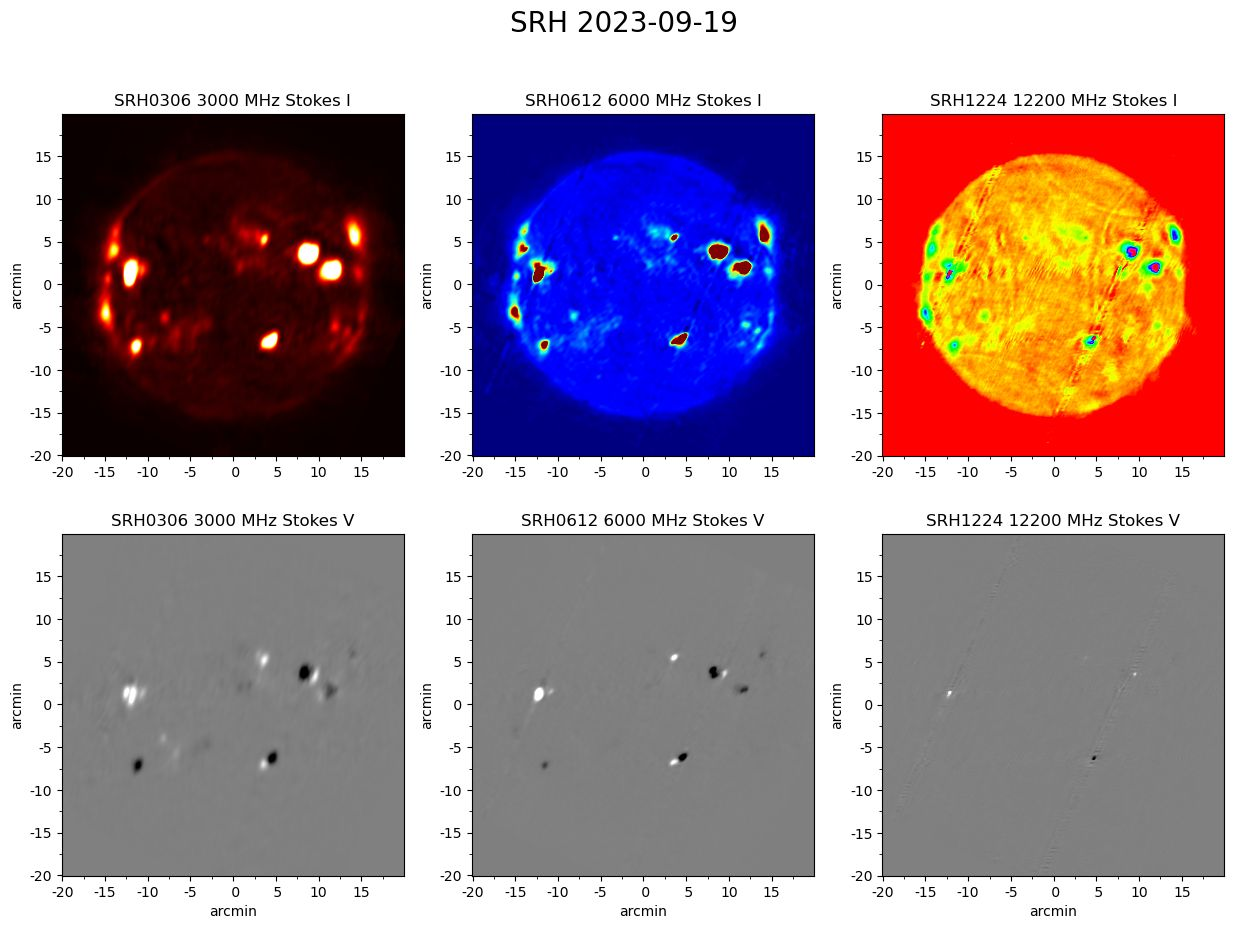
\includegraphics[scale=0.9]{images/img_example}
	\caption{Примеры изображений с разных решеток интерферометра: сверху представлена суммарная интенсивность правой и левой круговой поляризаций $I$, снизу -- их разность, параметр Стокса $V$}
	\label{fig:img_example}
\end{figure}

Как можно заметить из рис. \ref{fig:img_example}, на изображениях диапазона 12-24 ГГц имеются полосы -- подобный эффект наблюдается также и на данных наблюдений Нобеямского радиогелиографа, и является следствием неравномерного заполнения $UV$-плоскости.

\begin{figure}[H]
	\centering
	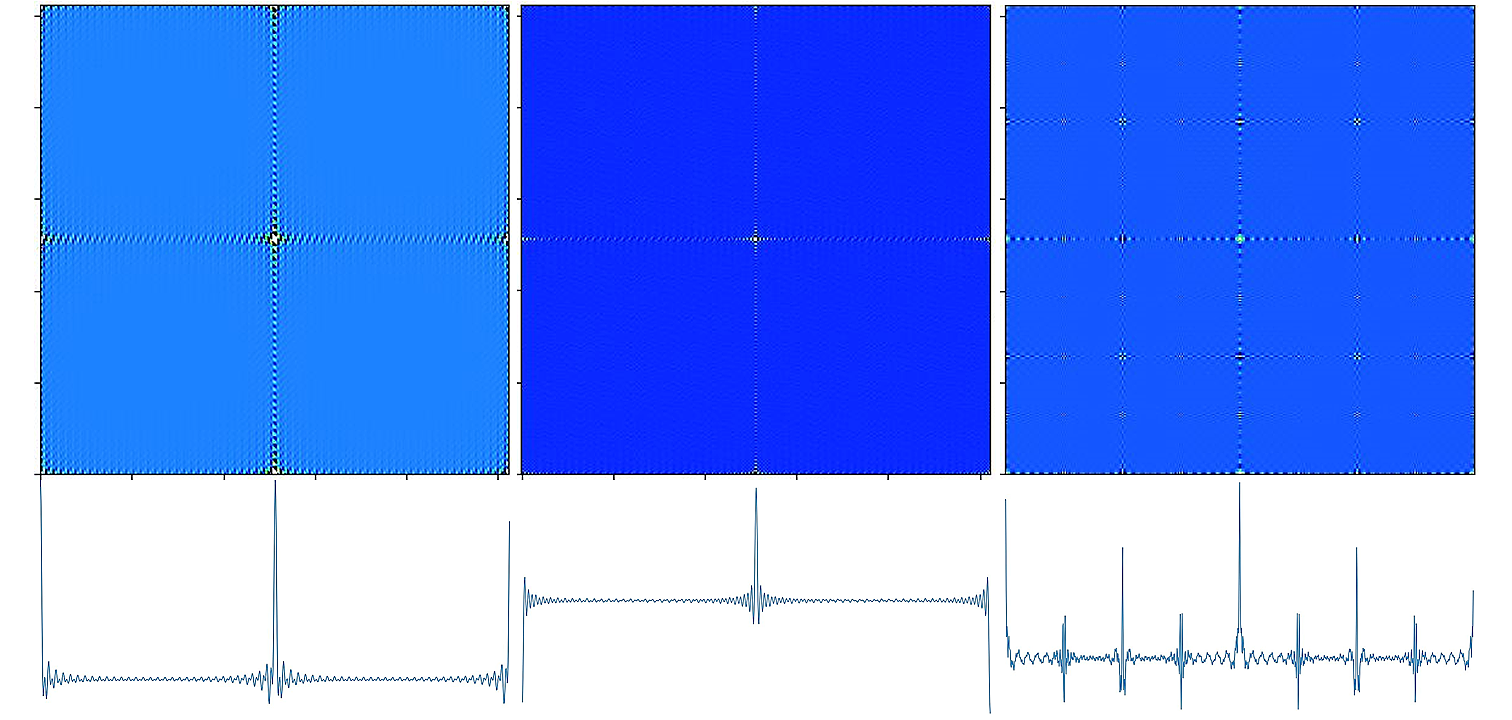
\includegraphics[scale=0.43]{images/psfs}
	\caption{Диаграммы направленности решеток интерферометра в системе координат направляющих косинусов}
	\label{fig:psfs}
\end{figure}

Из рисунка \ref{fig:psfs} видно, что вторичные максимумы диаграммы направленности для решеток 3-6 и 12-24 ГГц имеют положительный знак, а для решетки 6-12 ГГц -- отрицательный. Также видно еще одно следствие несимметричности лучей решетки 3-6 ГГц -- нерегулярная структура ее лепестков, а также следствие неэквидистантности антенн решетки 12-24 -- сложная структура ее диаграммы направленности, с дополнительными знакопеременными лепестками, от которых потом довольно сложно очищать изображение.

\subsection{Теорема Ван Циттерта-Цернике}
Основная теорема интеферометрии звучит так:
\newtheorem*{Van_Cittert_Zernike}{Теорема Ван Циттерта-Цернике}
\begin{Van_Cittert_Zernike}
Распределение интенсивности по углу связано с взаимной когерентностью падающего излучения через преобразование Фурье, т.е.:
\begin{equation}\label{eq:Ван Циттерт-Церник}
	\Gamma_{12} (u,v,0) = \iint I(l,m) e^{-2\pi i(ul+vm)} dl \, dm
\end{equation}
\end{Van_Cittert_Zernike}
\noindent $u$ и $v$ в формуле \ref{eq:Ван Циттерт-Церник} являются пространственными частотами, $l$ и $m$ -- направляющие косинусы. Эта система координат удобна, потому как в ней $UV$-плоскость и диаграмма направленности выглядят одинаково, а меняется только форма и размер источника.

\begin{figure}[H]
	\centering
	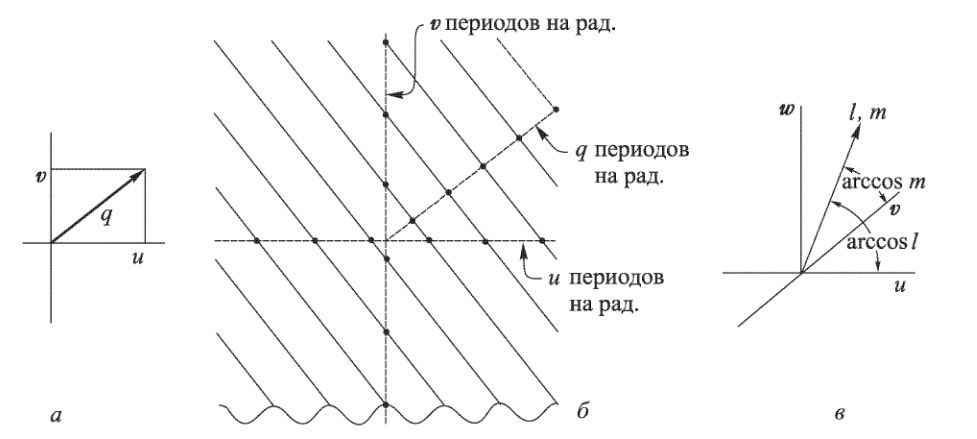
\includegraphics[scale=0.8]{images/cosinuses}
	\caption{К объяснению системы координат направляющих косинусов}
	\label{fig:cosinuses}
\end{figure}

Функция взаимной когерентности в данном случае определяется перемножением сигналов с пар антенн, произведение которых затем усредняется. В свою очередь, сигнал определяется видностями, которые связаны с распределением радиояркости на небе через преобразование Фурье (рис. \ref{fig:Van_Cittert_Zernike}).

\begin{figure}[H]
	\centering
	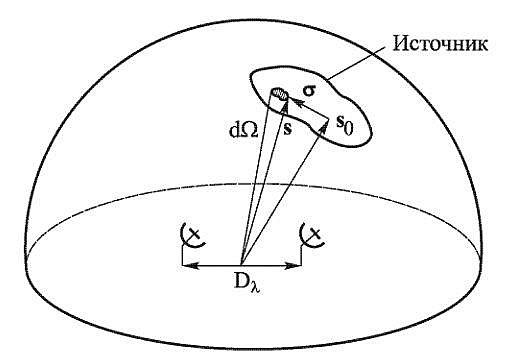
\includegraphics[scale=1]{images/Van_Cittert_Zernike}
	\caption{Схематическое пояснение теоремы Ван Циттерта-Цернике}
	\label{fig:Van_Cittert_Zernike}
\end{figure}

\subsection{Преобразование Фурье и теорема о свертке}
Пусть есть $a(t)$, $b(t)$, тогда
\begin{equation}\label{eq:Фурье А}
	A(\omega) =\int_{-\infty}^{\infty} a(t)exp(i \omega t) dt,
\end{equation}
\begin{equation}\label{eq:Фурье В}
	B(\omega) =\int_{-\infty}^{\infty} b(t)exp(i \omega t) dt
\end{equation}
-- Фурье-образы функций $a(t)$, $b(t)$.

\newtheorem*{Convolution_theorem}{Теорема о свёртке}
\begin{Convolution_theorem}
	Перемножение сигналов по времени равносильно сворачиванию их спектров, и наоборот
\end{Convolution_theorem}

Таким образом:
\begin{equation}\label{eq:ThConvolution1}
	a(t) \cdot b(t) = A(\omega) * B(\omega),
\end{equation}
\begin{equation}\label{eq:ThConvolution2}
	a(t) * b(t) = A(\omega) \cdot B(\omega)
\end{equation}

Операция же свертки представляет собой следующую процедуру:
\begin{equation}\label{eq:Convolution}
	(f * g)(t) := \int_{-\infty}^{\infty} f(\tau) g(t-\tau) d\tau
\end{equation}

\begin{figure}[H]
	\centering
	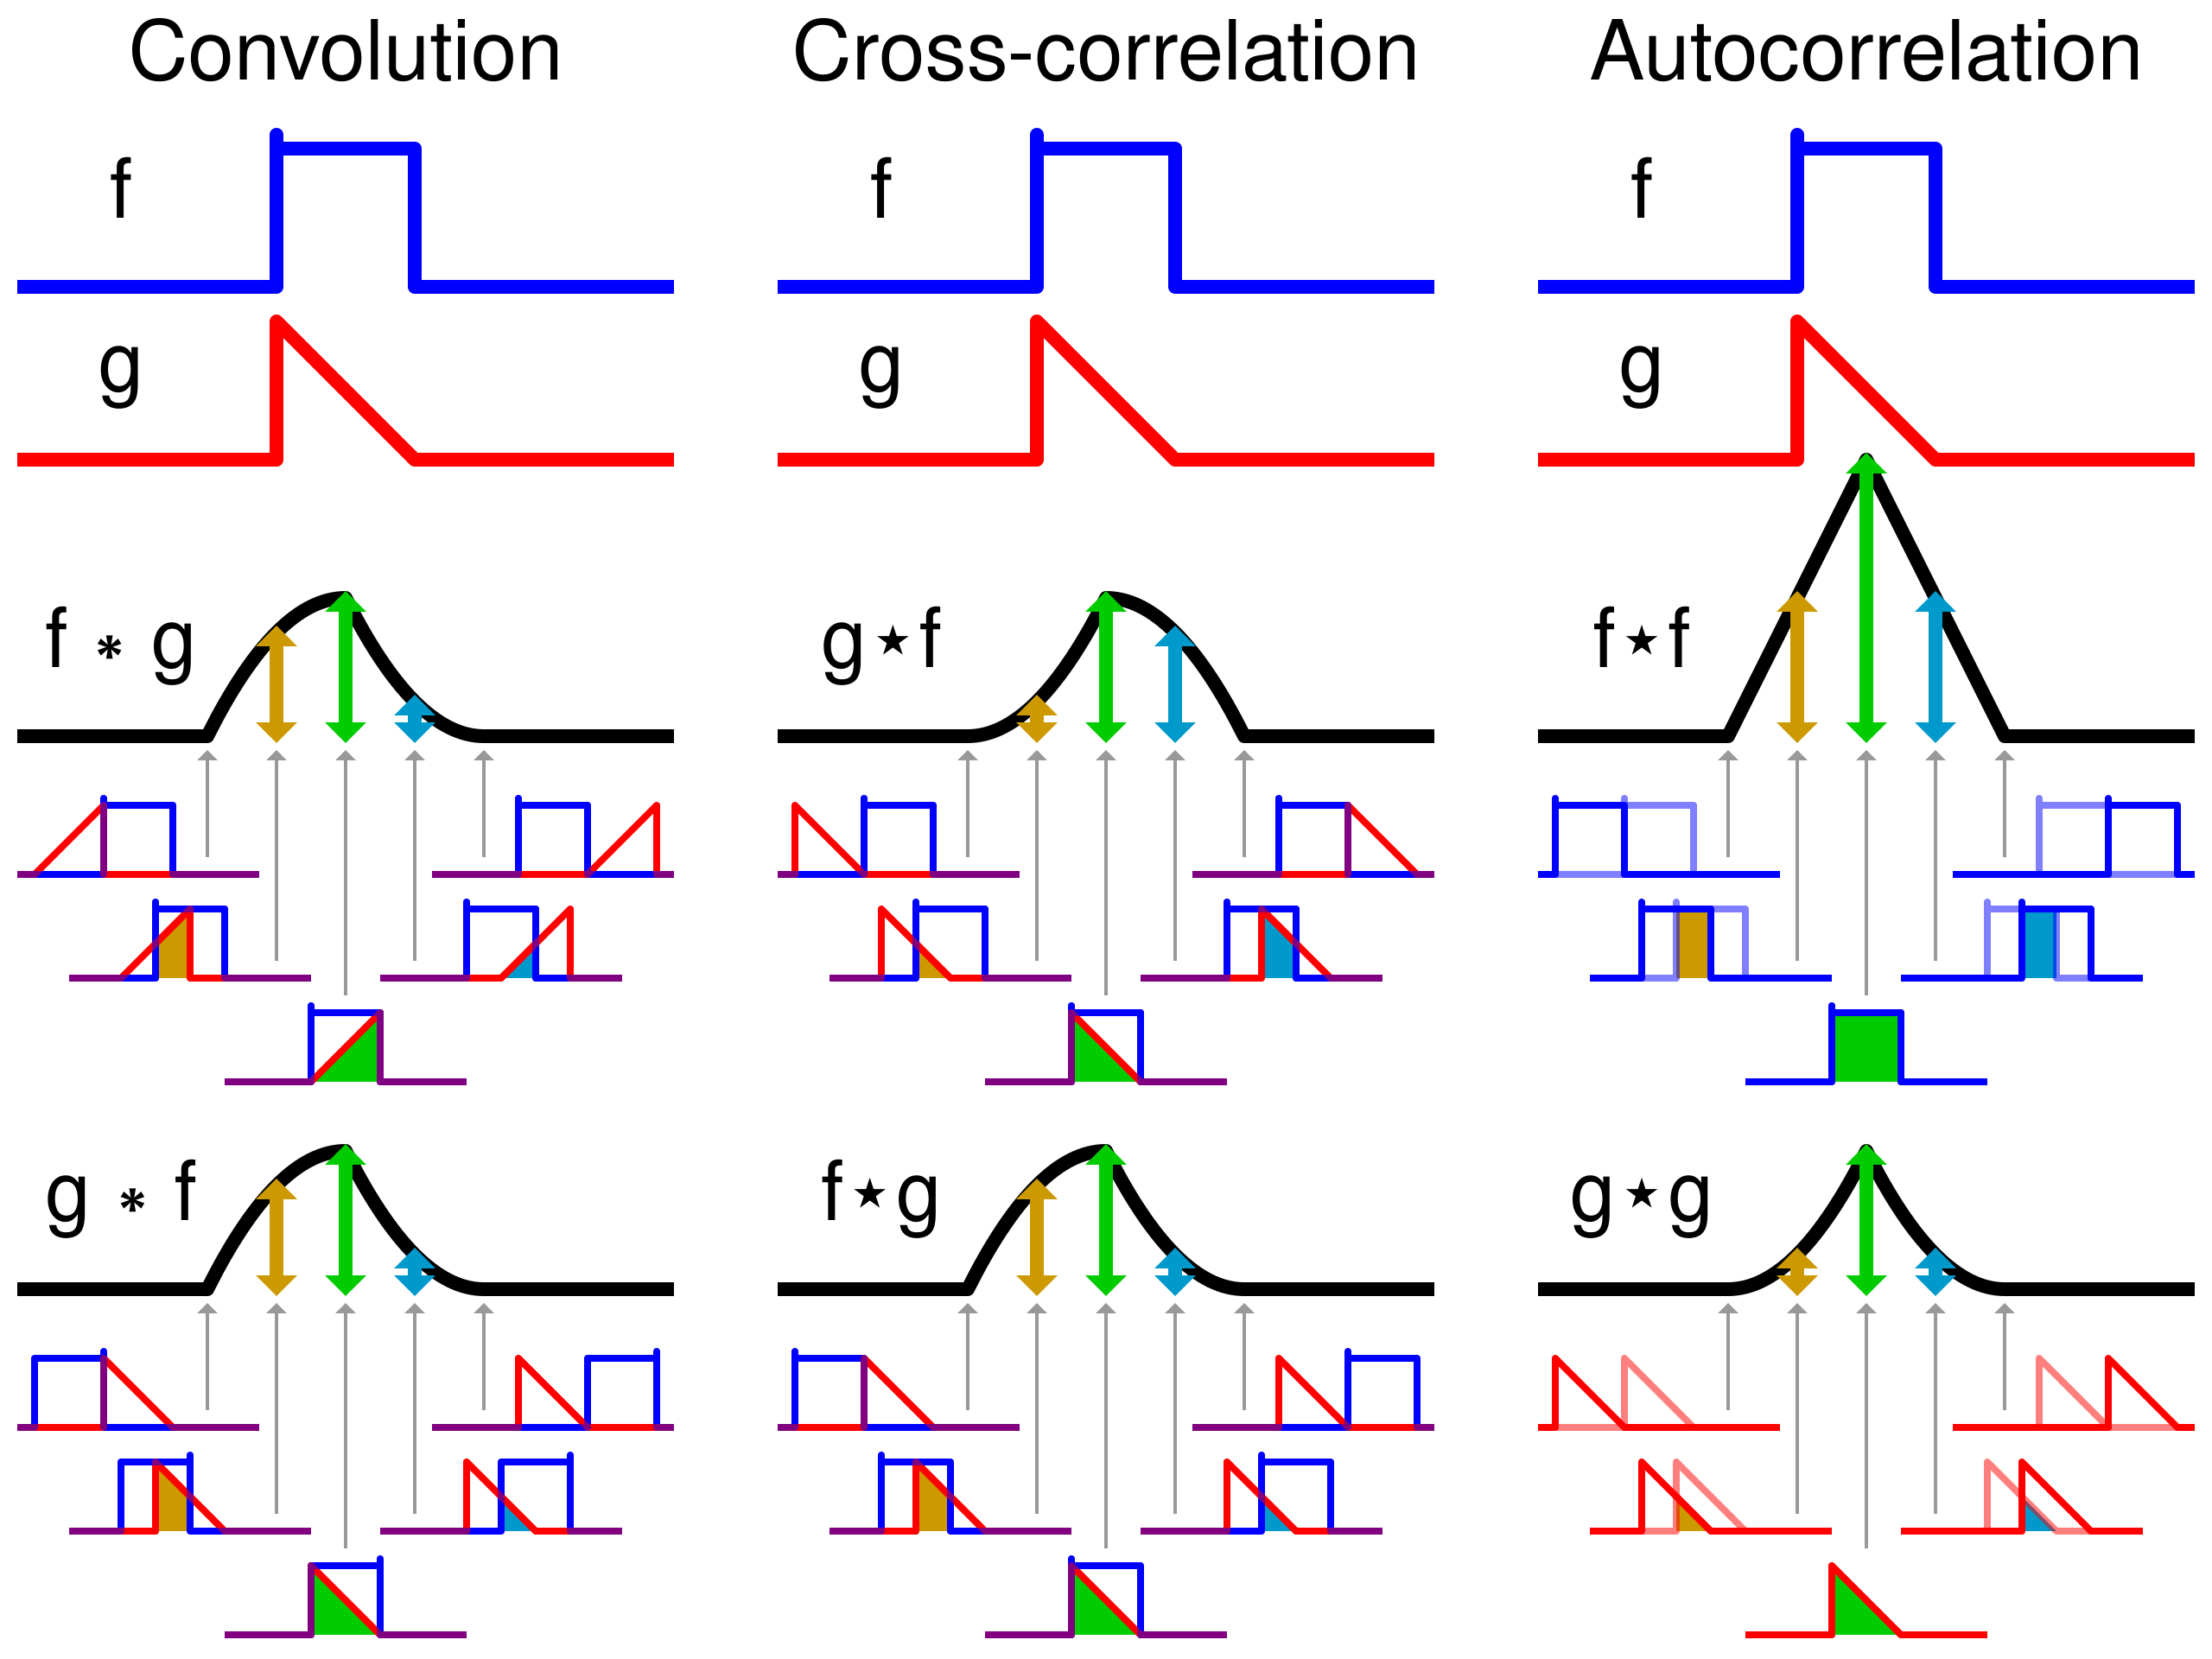
\includegraphics[scale=0.14]{images/Comparison_convolution_correlation}
	\caption{Визуальное сравнение свертки, взаимной корреляции и автокорреляции}
	\label{fig:Comparison_convolution_correlation}
\end{figure}

\noindent Функция, с которой происходит сворачивание, называется ядром свертки.

\begin{figure}[H]
	\centering
	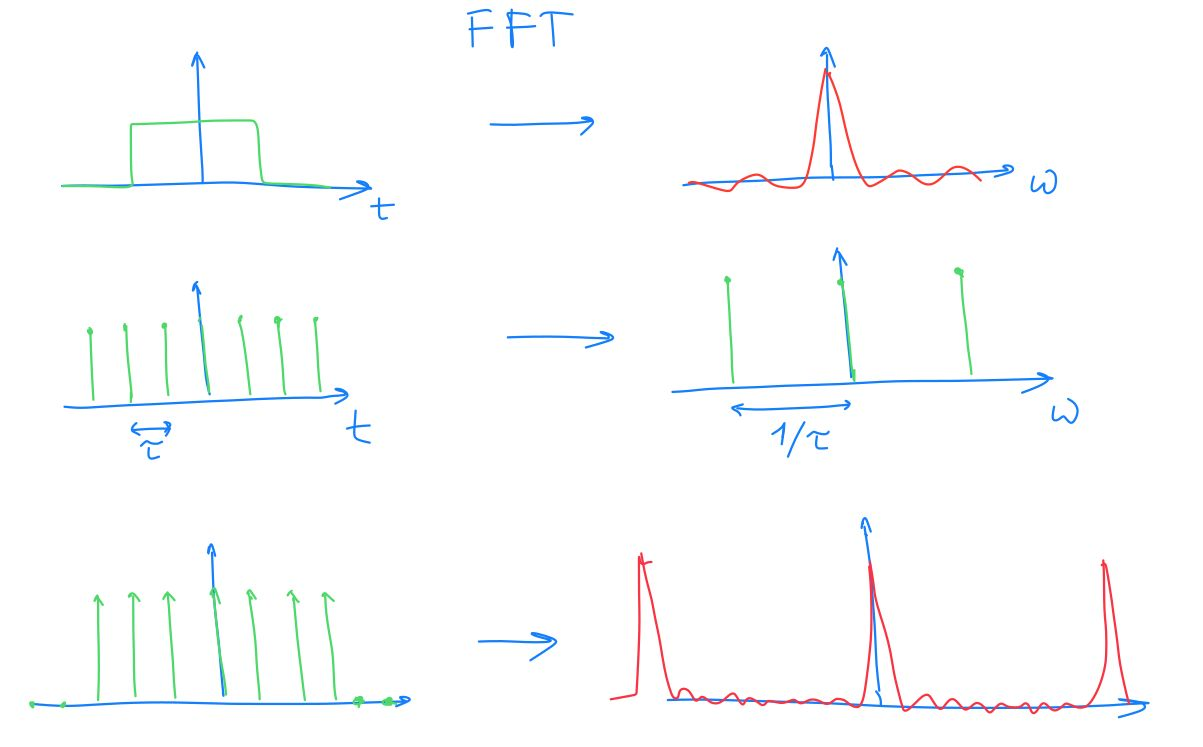
\includegraphics[scale=0.8]{images/FFT1}
	\caption{Пары сигнал - спектр}
	\label{fig:FFT1}
\end{figure}

\begin{figure}[H]
	\centering
	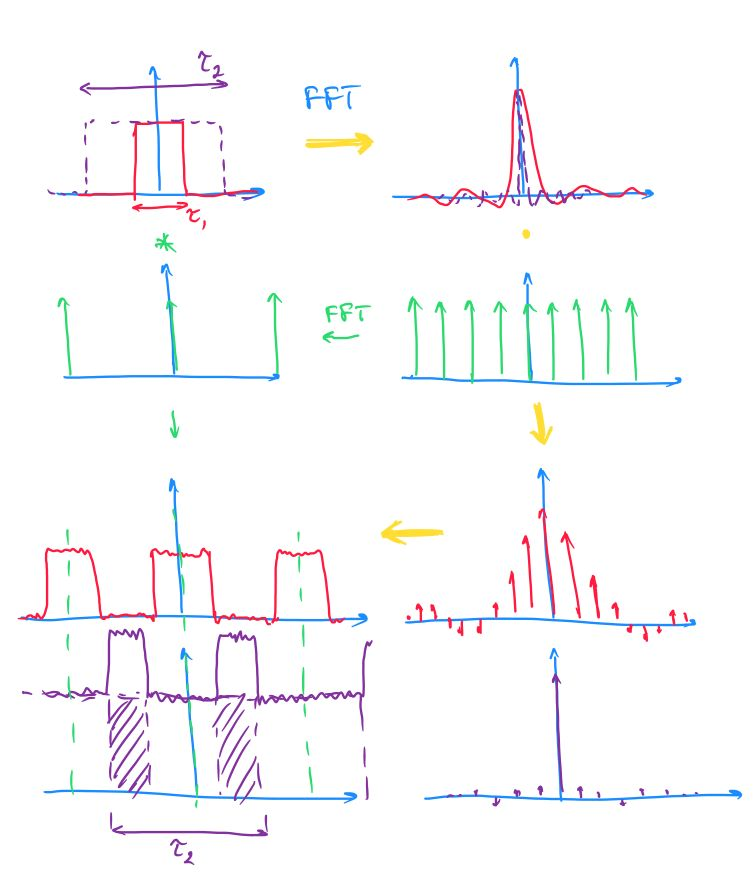
\includegraphics[scale=0.8]{images/FFT2}
	\caption{Пары сигнал - спектр}
	\label{fig:FFT2}
\end{figure}

\section{Введение}

\begin{figure}[H]
	\centering
	
\includegraphics[scale=0.55]{img/smile.png}
	\caption{гыгыгыгыгыгыгыгыгы}
	\label{fig:gygygy}
\end{figure}

Это шаблон учебного пособия, в котором можно показывать рисунки (см. рис. \ref{fig:gygygy})

\subsection{Делать подразделы}
Вот

\paragraph{Еще и параграфы}
И ссылаться на литературу \cite{priest}


%%!TEX root = ../lectionsA4.tex


\section{Введение}

Курс \textbf{механики сплошных сред}\footnote{Далее будем часто сокращать название дисциплины до <<МСС>>} является одним из разделов цикла теоретической физики.  В знаменитом курсе теоретической физики Л.Д.~Ландау и Е.М.~Лифшица  ему посвящено два достаточно объёмных тома \cite{nu1}.

Наш курс рассчитан на радиофизиков: он существенно меньше, чем курсы на специализированных факультетах, и в нём несколько больше внимания уделено волновым процессам.

Студентам радиофизического факультета курс электродинамики и курс МСС читаются в одном семестре. В этих дисциплинах возникают одинаковые уравнения: это одна из причин параллельного прочтения этих курсов, математический аппарат которых в основном базируется на формулах векторного анализа. Стоит отметить, что при этом уравнения МСС существенно сложнее уравнений электродинамики, где базовыми являются линейные уравнения Максвелла.

В списке литературы, представленном в конце книги, приведена основная литература по курсу \cite{nu1,nu2,nu3,nu4, nu5}, дополнительная литература по курсу \cite{nu6, nu7, nu8, nu9, nu10, nu11, nu12, nu13, nu14}, а также монографии, учебники и статьи для углублённого знакомства с отдельными разделами курса.

\subsection{Исторический экскурс}
\textbf{Механика сплошных сред}~--- одна из древнейших наук. Её зарождение началось ещё в античной древности.

История развития МСС полностью подтверждает наличие тесной связи между становлением науки и запросами практики.

Фамилии (но не годы жизни) известных учёных, сделавших вклад в развитие МСС, знают все. Это:
\begin{itemize}
	\setlength\itemsep{-0.4em}
	\item Аристотель (384--322 г.г. до н.э.)
	\item Архимед (287--212 г.г. до н.э.)~--- закон Архимеда
\end{itemize}
	Средние века:
\begin{itemize}
	\setlength\itemsep{-0.4em}
	\item Галилей (1564--1642)
	\item Паскаль (1623--1662)
	\item Леонардо да Винчи (1452--1519).
	Это и летательные аппараты, закон Паскаля для давления, наблюдение гидродинамической турбулентности.
	\item Гюйгенс (1629--1695)
	\item Ньютон (1642--1727). В своих знаменитых \emph{<<Началах>>} он приводит теоретический вывод квадратичного закона сопротивления. Именно из законов Ньютона было проведено обобщение на сплошные среды и родилась новая наука~--- гидромеханика.
\end{itemize}
Это два академика Российской академии наук:
\begin{itemize}
	\setlength\itemsep{-0.4em}
	\item Леонард Эйлер (1707--1789)~--- уравнение Эйлера
	\item Даниил Бернулли (1700--1782)~---  уравнение Бернулли
\end{itemize}
Начало XIX века:
\begin{itemize}
	\setlength\itemsep{-0.4em}
	\item Даламбер (1717--1783)~--- парадокс Даламбера
	\item Лагранж (1736--1813)
	\item Коши (1789--1857)
\end{itemize}
Вязкая жидкость:
\begin{itemize}
	\setlength\itemsep{-0.4em}
	\item Анри Навье  (1785--1863)
	\item Стокс (1819--1903)~--- уравнение Навье--Стокса
\end{itemize}
Эксперименты с жидкостью:
\begin{itemize}
	\setlength\itemsep{-0.4em}
	\item Ж. Пуазейль (1799--1869)
\end{itemize}
Основы теории турбулентности:
\begin{itemize}
	\setlength\itemsep{-0.4em}
	\item Осборн Рейнольдс (1842--1912)
	\item Н.Е. Жуковский (1847--1921)~--- обтекание крыла, присоединённый вихрь, подъёмная сила
	\item С.А. Чаплыгин (1869--1942)
	\item Морис Мари Альфред Куэтт  (1858--1943)~--- течение Куэтта
\end{itemize}
Теория турбулентности и теория устойчивости:
\begin{itemize}
	\setlength\itemsep{-0.4em}
	\item Людвиг Прандтль  (1875--1953)
	\item Теодор Карман (1881--1963)
	\item Колмогоров А.Н.  (1903--1987), \\Обухов А.М.   (1918--1989)~---  Закон Колмогорова--Обухова.
\end{itemize}

Практически все эти фамилии будут встречаться в нашем курсе. Их именами названы законы {МСС}.

В наше время бурное развитие получила вычислительная {МСС}. Так, ни один новый самолёт не получит разрешение на эксплуатацию, если не будет построена его математическая модель, включающая процессы обтекания самолёта потоком воздуха.

Что же включает современная {МСС}? Книга академика Л. Седова <<Краткое перечисление современных проблем>> включает 21 пункт и занимает 4 страницы \cite{nu10}. Здесь мы приведем лишь те, которые тесно связаны с предприятиями и НИИ Нижнего Новгорода, на которых работают выпускники радиофизического факультета ННГУ.

\begin{enumerate}
	\item Изучение движения жидкости и газа~--- движение самолётов, вертолётов, подводных лодок.  Возникновение турбулентных следов за объектами. Излучение звука винтами и турбулентными струями.
	\item Движение жидкости и газа в трубах. Взаимодействие волн в оболочках.
	\item Волновые движения в жидкостях и газах:
	\begin{itemize}
		\item Волны в твёрдых телах.  Акустическая диагностика, взаимодействие с электромагнитными волнами~--- линии задержки на ПАВ\footnote{ПАВ~--- поверхностные акустические волны}.
		\item Волны на поверхности моря и внутренние волны, их нелинейное взаимодействие. Обнаружение подводных лодок по изменению характеристик поверхностного волнения.
		\item Волны в каналах, реках. Генерация цунами и  набег волн цунами на берег.
		\item Сейсмические процессы, нелинейная сейсмодиагностика.
		\item Звуковые волны,  гидроакустика, акустика океана.
	\end{itemize}
	\item Теория турбулентности~--- гравитационная неустойчивость.
	\item Биологическая механика, движение крови в сосудах, диагностика на различных типах волн~--- сдвиговые волны.
\end{enumerate}

В Нижнем Новгороде работает один из крупнейших институтов Российской академии наук~--- \href{https://www.ipfran.ru}{\textit{Институт прикладной физики}}\footnotemark, тесно занимающийся широким спектром задач, часть из которых изучается в нашем курсе.

ИПФ РАН входит в структуру Нижегородского научного центра РАН, в который также входят \textit{Институт физики микроструктур РАН} и \textit{Институт проблем машиностроения РАН}.

\footnotetext{
\textbf{Федеральное государственное бюджетное научное учреждение <<Федеральный исследовательский центр Институт прикладной физики Российской академии наук>> (ИПФ РАН)} был создан на базе нескольких отделов Научно-исследовательского радиофизического института (НИРФИ) Минвуза РСФСР в апреле 1977~года. Основатель и директор института на протяжении первых 25 лет его работы~--- академик А.В.~Гапонов-Грехов, с 2003 по 2015~год институт возглавлял академик А.Г.~Литвак, с 2015~года до своего избрания президентом РАН в 2017 году директором института был академик А.М.~Сергеев. С 2019~г.  директором ИПФ РАН избран академик РАН Г.Г.~Денисов.
}


% \newpage
\subsection{Основные допущения МСС}
Вещество можно рассматривать как непрерывную сплошную среду, пренебрегая его молекулярным строением, и считать распределение всех характеристик жидкости (плотность, скорость, температура, $\ldots$) непрерывным.
%
Это означает, что всякий малый элемент жидкости или газа содержит большое число молекул (или других частиц). То есть когда мы говорим о бесконечно малом элементе жидкости, то везде мы подразумеваем,  что \textit{<<физически>> бесконечно малый объём} мал по сравнению с размерами тел, но велик по сравнению с межмолекулярными расстояниями.
%
Это позволяет применить в МСС хорошо разработанный для непрерывных функций аппарат высшей математики.

Нетривиальный пример применения МСС~--- \textbf{крупномасштабная структура  Вселенной.} Оказывается, описать развитие крупномасштабной структуры можно уравнениями гидродинамики газа гравитационно взаимодействующих частиц. Здесь \emph{<<физически>> бесконечно малый объём}~--- это объём, в котором содержится много галактик.

Существующие на данный момент крупномасштабные образования возникли из-за малых начальных возмущений плотности за счёт гравитационной неустойчивости. Из чего состоит Вселенная: обычная материя (атомы различных веществ) (4\%), Темная материя неизвестной физической природы (cold dark matter) (23\%). Темная энергия (dark energy) (73\%), которая играет антигравитационную роль в процессе формирования Вселенной.

Плотность тёмного вещества в 6--7 раз превосходит плотность барионов, и поэтому рост неоднородностей определяется в основном темным веществом. Именно рост неоднородностей в тёмном веществе и ответственен за формирование крупномасштабных структур. Барионная компонента просто следовала за эволюцией тёмного вещества.

В космологии понятие крупномасштабной структуры относится к распределению галактик и массы тёмного вещества (на масштабах от одного до нескольких сотен мегапарсек\footnote{1 Mpc = $10^6$ pc $\approx$ 3\,260\,000 световых лет}). Современная теория объясняет формирование крупномасштабной структуры Вселенной как следствие роста исходных слабых флуктуаций плотности вещества за счёт гравитационной неустойчивости. При этом формирование ярко выраженных элементов структуры происходит на нелинейной стадии. Именно поэтому процесс формирования крупномасштабной структуры принято иногда называть гравитационной турбулентностью.

Наиболее очевидный путь преодоления сложности учёта законов нелинейной эволюции гравитационной неустойчивости в поведении поля плотности вещества состоит в численном моделировании трёхмерного движения $N$ гравитационно взаимодействующих частиц. Альтернативой являются приближенные аналитические решения некоторых уравнений в частных производных, адекватно описывающих рост флуктуаций неоднородной плотности вещества в расширяющейся Вселенной. Первый из этих подходов был предложен Зельдовичем в 1970 году.

Второй аналитический подход к проблеме описания формирования крупномасштабной структуры Вселенной \cite{a1} базируется на векторном уравнении Бюргерса. В данном подходе многопотоковое движение гравитационно взаимодействующих частиц в особенностях, приводящих к их локализации, моделируется вязким слагаемым в уравнении Бюргерса. В предельном случае исчезающе малой вязкости это эквивалентно слипанию частиц, и поэтому данный подход часто называют приближением слипания~--- adhesion model \cite{a2,a3,a4,a5}.
Предельная версия модели слипания естественным образом описывает характерную мозаичную структуру распределения вещества во Вселенной. Основные элементы <<мозаики>> в трёхмерном пространстве (вершины, рёбра, грани и внутренности ячеек) могут быть ассоциированы с наблюдаемыми структурами трёхмерного распределения галактик (компактные скопления галактик, филаменты~--- цепочки галактик, поверхности со сравнительно высокой плотностью галактик и темные области между ними, бедные галактиками).
% Adhesion model Модель Зельдовича--Гурбатова--Саичева

\begin{figure}[H]
	\centering
	\includegraphics[width=.48\textwidth]{photo/1}
    \includegraphics[width=.48\textwidth]{photo/2_}
	\caption{Крупномасштабная структура Вселенной (слева) и система каустик на дне бассейна (справа)}
	\label{fig:krup_mash}
\end{figure}

Сама эволюция крупномасштабной структуры Вселенной может трактоваться как непрерывный процесс транспортировки вещества преимущественно из объектов большой размерности к объектам мозаичной структуры, обладающим меньшей размерностью. К примеру, вещество из внутренних ячеек мозаичной структуры (трёхмерных объектов) перетекает в её грани (квазидвумерные объекты), а из них в рёбра и вершины мозаичной структуры. В то же время, сами ячейки участвуют в непрерывном движении, деформации и поглощении одних ячеек другими.

% \begin{figure}[H]
% 	\centering
% 	\includegraphics[width=.5\linewidth]{photo/2}
% 	\caption{}
% 	\label{fig:figure2}
% \end{figure}

Формирование особенностей гравитационно взаимодействующих частиц близко по своей физике процессу возникновения каустик при прохождении оптической волны через фазовый экран \cite{a4,a5,a60}. На рис.~\ref{fig:krup_mash} приведена картина оптических каустик на дне бассейна с взволнованной поверхностью.

В заключение отметим, что результаты динамического моделирования в рамках приближения слипания можно \href{https://www.youtube.com/watch?v=wI12X2zczqI}{посмотреть на YouTube} \cite{sticky1}.
% (\textbf{The Sticky Geometry of the Cosmic Web, version 2.01})
%
% \url{https://www.youtube.com/watch?v=wI12X2zczqI}

Результаты прямого численного моделирования (N-body simulation) можно также  посмотреть на YouTube, как для \href{https://www.youtube.com/watch?v=nHvcqV92oqY}{двумерного} \href{https://www.youtube.com/watch?v=74IsySs3RGU}{случая} \cite{nbody2d_1,nbody2d_2}, так и для \href{ttps://www.youtube.com/watch?v=eDGtFRj4xXc}{трёхмерного} \cite{nbody3d}.

% Двухмерный случай:

% \url{https://www.youtube.com/watch?v=nHvcqV92oqY}

% \url{https://www.youtube.com/watch?v=74IsySs3RGU}

% Трехмерный случай

% \url{https://www.youtube.com/watch?v=eDGtFRj4xXc}


\newpage
\section{Гидродинамика идеальной жидкости}
% \begin{tikzpicture}[remember picture,overlay]
%     \coordinate (A) at (current page.north west);
%     \coordinate (B) at (current page.south east);
%     \draw[red, very thick]%, cap=round]
%         ($(A)+(20mm, -20mm)$) rectangle ($(B)+(-20mm, 20mm)$);
% \end{tikzpicture}
В  данном разделе мы рассмотрим законы движения и равновесия идеальной жидкости, то есть жидкости, в которой не учитывается внутреннее трение, и, следовательно, нет перехода механической энергии в тепловую. Будем также пренебрегать теплообменом между  различными объёмами жидкости.

Это означает, что все процессы протекают при постоянной энтропии, а состояние жидкости характеризуется одной скалярной величиной~---  давлением $p$. Это, конечно, идеализация, которая приводит к ряду парадоксальных результатов (например, парадокс  Даламбера--Эйлера~---  сила сопротивления при равномерном движении тела в жидкости равна нулю). Тем не менее, без этой идеализации невозможно дальнейшее изучение реальных ситуаций.

\subsection[Основные уравнения гидродинамики\newline идеальной жидкости]{Основные уравнения гидродинамики идеальной жидкости}
Прежде чем перейти к выводу уравнений, рассмотрим два альтернативных способа описания движения жидкости. Оба они были предложены Леонардом Эйлером, но один из них носит имя Лагранжа.

\index{Описание!Лагранжа}
\paragraph{Лагранжево описание.} В основу этого способа положено описание движения отдельных <<жидких частиц>>. Все величины, в том числе и  координаты частиц жидкости, определяются как функции времени $t$  и некоторых переменных $\xi_k$ $(k=1,2,3)$, идентифицирующих определенную частицу (<<метки>> частиц):
\begin{equation}
	x_i =x_i(\xi_k,t), \quad
	P =P(\xi_k,t), \quad
	\rho = \rho(\xi_k,t), \quad \ldots.
\end{equation}
В качестве переменных $\xi_k$ обычно используют начальные координаты частиц жидкости
\begin{equation}
	% t &=t_0 \\
	\xi_i = x_i(\xi_k, t_0).
\end{equation}

Таким образом, при Лагранжевом описании мы следим за определёнными частицами жидкости и смотрим, как изменяются во времени их координаты,  скорости, ускорения, а также давление, температура, плотность в их окрестности.\\
При этом скорости $\vec{v}$ и ускорения $\vec{a}$ частиц вычисляются по формулам
\begin{equation}
	v_{i} =\frac{\partial x_{i}}{\partial t}, \quad
	a_{i} =\frac{\partial^{2} x_{i}}{\partial t^{2}}.
\end{equation}
Здесь $ \vec{v}\left(\xi_{k}, t\right) $~--- скорость частицы в момент времени $t$, которая в начальный момент имела координаты $\xi_1$, $\xi_2$, $\xi_3$.

Отметим, что такому описанию соответствует способ исследования реки с помощью геофизических буев с нулевой плавучестью (см. рис. \ref{fig:figure3}).
\begin{figure}[H]
	\centering
	\includegraphics[scale=1]{photo/3.pdf}
	\caption{Схематичная картина Лагранжева и Эйлерова описания}%. \ding{58} - якорь.}
	\label{fig:figure3}
\end{figure}
\index{Описание!Эйлера}
\paragraph{Эйлерово описание.} В этом случае неподвижное пространство заполнено движущейся жидкостью. Движение жидкости будет определено, если все величины, характеризующие жидкость (скорость движения, давление, плотность, температура и т.д.) \textit{будут известны в любой точке пространства в любой момент времени}.
Это означает, что мы можем проследить, как изменяются эти величины от точки к точке:
\begin{equation}
	\vec{v} =\vec{v}(\vec{x}, t), \quad
	T = T(\vec{x}, t).
\end{equation}
% Система заякоренных буев.
В Эйлеровом описании мы не знаем, что делается с отдельной частицей.

При этом частные производные от скорости не являются ускорением. Так, если течение стационарно и частная производная по времени  равна нулю, частицы в данной точке могут иметь ускорение. Пример --- водопад.

Найдём ускорение частицы. За время $ \Delta t $ частица, находящаяся в момент времени $t$ в точке с координатами $ x_{k} $, переместится в точку $ x_{k}=x_{k}+\Delta x_{k} $. Тогда для $i$-ой компоненты ускорения имеем
\begin{equation}
\lim_{\Delta t \rightarrow 0} \frac{\Delta x_{k}}{\Delta t} =\frac{\partial x_{k}}{\partial t}=v_{k},
\end{equation}
\begin{equation}\begin{aligned}
	a_{i} &=\lim _{\Delta t \rightarrow 0} \frac{v_{i}\left(x_{k}+\Delta x_{k}, t+\Delta t\right)-v_{i}\left(x_{k}, t\right)}{\Delta t} = \\
	&=\lim _{\Delta t \rightarrow 0}\frac{\left[v_{i}\left(x_{k}, t\right)+\frac{\partial v_{i}}{\partial x_{k}} \Delta x_{k}+\frac{\partial v_{i}}{\partial t}\Delta t-v_{i}\left(x_{k}, t\right)\right]}{\Delta t} =\frac{\partial v_{i}}{\partial x_{k}} v_{k}+\frac{\partial v_{i}}{\partial t}.
\end{aligned}\end{equation}
Таким образом,
\begin{equation}
a_{i} =\frac{\partial v_{i}}{\partial t}+v_{k} \frac{\partial v_{i}}{\partial x_k}=\left(\pdv{t}+v_{k} \pdv{x_k}\right) v_{i},
\end{equation}
или в векторной форме
\begin{equation}
	\vec{a} =\frac{\partial \vec{v}}{\partial t}+(\vec{v}\,\nabla) \vec{v}=\left(\pdv{t}+(\vec{v}\,\nabla)\right) \vec{v}.
\end{equation}

Аналогично находятся и производные от любой другой величины. Эта производная носит название \textit{субстанциональной производной}:
\index{Производная!субстанциональная}
\index{Производная!локальная}
\begin{equation}
\dv{t}=\pdv{t}+(\vec{v}\,\nabla).
\end{equation}
Первое слагаемое здесь~--- \textit{локальная производная}.


\subsection{Связь Лагранжева и Эйлерова описаний}
Пусть нам известно Эйлерово поле скорости $ \vec{v}=\vec{v}\qty(\vec{x}, t) $. Чтобы найти, как двигаются Лагранжевы частицы $ \vec{X}\qty(t, \vec{\xi}\,) $, нам нужно решить уравнение
\begin{equation}
\dv{\vec{X}}{t}=\vec{v}\qty(\vec{X}, t), \qquad
\vec{X}\qty(t=0, \vec{\xi}\,)=\vec{\xi}.
\end{equation}
Как найти Эйлерово поле скорости? Если нам известны координаты частиц в Лагранжевом описании $ \vec{X}(t, \vec{\xi}\,) $ и их скорость $ \vec{V}(t, \vec{\xi}\,) $, то вначале нам нужно решить уравнение
\begin{equation}
\vec{x}=\vec{X}\qty(t, \vec{\xi}\,).
\end{equation}
Решение этого уравнения $\vec{\xi}=\vec{\xi}\qty(\vec{X}, t)$
позволяет найти Лагранжеву частицу, которая в момент времени $t$ попала в точку $x$. Отсюда в Эйлеровом представлении
\begin{equation}
\vec{v}(\vec{x}, t)=\vec{V}\qty(t, \vec{\xi}(\vec{x}, t)).
\end{equation}




\index{Уравнение!непрерывности}
\index{Закон!сохранения массы}
\subsection{Уравнение непрерывности и закон сохранения массы}
Пусть имеется некоторый объём пространства $V$, заполненный движущейся  жидкостью. Количество жидкости (масса) в этом объёме:
\begin{equation}
m=\int\limits_{V} \rho\dd{V}\!,
\end{equation}
где $\rho$ --- плотность жидкости. Жидкость может притекать и вытекать из объёма. Введём элемент поверхности $ \dd\sigma $ и вектор $ \dd \vec{\sigma}=\dd\sigma \vec{n} $, направленный по внешней нормали к поверхности (см. рис. \ref{fig:vvn}).
\begin{figure}[H]
	\vspace{-10pt}
	\centering
	\includegraphics[scale=1]{photo/4.pdf}
	\caption{Объем, скорость и нормаль к поверхности}
	\label{fig:vvn}
\end{figure}
\noindent Поток через элемент поверхности определяется скалярным произведением
\begin{equation}
\oint\limits_{S} \rho \vec{v}\, \dd\vec{\sigma}.
%=\int\limits_{V} \Div(\rho \vec{v}\,)\dd{V}
\end{equation}
Уравнение баланса имеет вид:
\begin{equation}\begin{aligned}
\pdv{t} \int\limits_{V} \rho\dd{V}=-\oint\limits_{S} \rho \vec{v} \dd\vec{\sigma}.
\end{aligned}\end{equation}
Это интегральный закон сохранения массы. Если на поверхности скорость равна нулю, то масса сохраняется.

Используя формулу Остроградского--Гаусса
\begin{equation}\begin{aligned}
\oint\limits_{S} \rho \vec{v}\, \dd \vec{\sigma}=\int\limits_{V} \Div (\rho \vec{v}\,)\dd{V},
\end{aligned}\end{equation}
получим
\begin{equation}\begin{aligned}
\int\limits_{V}\left[\frac{\partial \rho}{\partial t}+\Div(\rho \vec{v}\,)\right]\dd{V}=0.
\end{aligned}\end{equation}

Так как объём произвольный, то мы получаем дифференциальный закон сохранения
\begin{equation}\begin{aligned}
\frac{\partial \rho}{\partial t}+\Div(\rho \vec{v}\,)=0.
\end{aligned}\end{equation}

Вектор $ \vec{j}=\rho \vec{v} $ --- плотность потока массы. Используя определение субстанциональной производной и учитывая, что
\begin{equation}
	\nabla(a\, \vec{b}\,)=\vec{b} \nabla a +a \nabla \vec{b},
\end{equation}
перепишем закон сохранения массы в виде:
\begin{equation}\begin{aligned}
\frac{\partial \rho}{\partial t}+(\vec{v}\,\nabla) \rho+\rho \Div(\vec{v}\,)=0
\quad \Rightarrow \quad \frac{\dd \rho}{\dd t}=-\rho \Div(\vec{v}\,).
\end{aligned}\end{equation}

\textbf{Несжимаемая жидкость~--- плотность частицы вдоль траектории  не меняется:}
\begin{equation}\begin{aligned}
\frac{\dd \rho}{\dd t}=0.
\end{aligned}\end{equation}
Это означает, что поле скорости соленоидальное: $\Div\vec{v}=0$.

\index{Уравнение!Эйлера}
\subsection{Уравнение Эйлера}
Уравнение Эйлера описывает движение идеальной жидкости и является аналогом второго закона Ньютона классической механики. Запишем его для жидкого элемента:
\begin{equation}\begin{aligned}
\rho\dd{V} \frac{\dd \vec{v}}{\dd t} =\vec{F_{S}}+\vec{F}, \qquad
\vec { F } = \rho \dd{V} \vec { f }.
\end{aligned}\end{equation}
Здесь $\vec{F}$~---  объёмная сила, действующая на элемент $\dd V$\!, $\vec{f}$~--- сила, отнесённая к единице массы (плотность силы), для силы тяжести $\vec{f}=\vec{g}$, где $g$~--- ускорение свободного падения.

Поверхностная же сила $\vec{F}_s$  действует на элемент объёма со стороны окружающей среды.  В идеальной среде силы трения нет, и единственная сила, действующая на поверхность, это сила давления. На элемент поверхности $\dd\sigma$ действует сила $p \dd{\vec{\sigma}}$, и результирующая сила равна
\begin{equation}
\vec { F } _ { S } = - \oint \limits_ { S } p \dd{\vec{\sigma}} = - \int \limits_ { V } \nabla p\dd{V} \approx - \nabla p\dd{V}.
\end{equation}
Здесь мы учли, что элемент $\dd{V}$ достаточно мал, и внутри него градиент давления практически постоянен. В результате получаем \textit{уравнение Эйлера}:
\begin{equation}
\begin{aligned}
    \dv{\vec{v}}{t} &= - \frac { \nabla p } { \rho } + \vec { f }, \qq{или}\\
    \frac { \partial \vec { v } } { \partial t } + ( \vec{v}\,\nabla ) \vec { v }  &=	- \frac { \nabla p } { \rho } + \vec { f }.
\end{aligned}
\end{equation}
Здесь мы учли, что в уравнение Ньютона входит полная производная.

У нас  5 неизвестных: 3 компоненты скорости, давление и плотность. А есть только 4 уравнения: 3 уравнения Эйлера для трёх компонент и уравнение непрерывности. Нужны ещё уравнение состояния, связывающее давление, плотность и энтропию $S$
\begin{equation}
	p = p(\rho,S),
\end{equation}
а также уравнение для энтропии. Для изоэнтропической жидкости
\begin{equation}
	\frac {\dd{S} } { \dd t } = \frac { \partial S } { \partial t } + \vec{v}\,\nabla S = 0.
\end{equation}
Если в начальный момент времени энтропия одинакова во всём пространстве, то она не меняется с течением времени, и уравнение состояния принимает вид $p = p ( \rho )$.

В идеальном газе уравнение адиабаты имеет вид \textit{уравнения Пуассона}:
\index{Уравнение!Пуассона}
\begin{equation}\begin{aligned}
p = p_0 \left( \frac{\rho}{\rho_0} \right) ^ { \gamma }, \qq{где}
\gamma = \frac{c_p}{c_v}.
\end{aligned}\end{equation}
Для идеального газа $\gamma = \frac{i+2}{i}$, где $i$~--- количество степеней свободы.


Для жидкостей дело обстоит сложнее: в разных диапазонах давления имеют место быть разные уравнения состояния. Эмпирическая формула для давления $p$, измеряемого в атмосферах:
\begin{equation}
\frac { p + B } { 1 + B } = \left( \frac { \rho } { \rho_0 } \right) ^ { \gamma }\!\!,
\end{equation}
где $B=3000\text{ атм}$, $\gamma = 7$, давление до $10^5$ атмосфер.

Итак, \textbf{система уравнений для идеальной жидкости} принимает вид:
\begin{equation}\begin{aligned}
& \frac { \partial \vec{v} } { \partial t } + ( \vec{v}\,\nabla ) \vec{v} = - \frac { \nabla p } { \rho } + \vec { f }, \\
& \frac { \partial \rho } { \partial t } + \Div ( \rho \vec{v}\,) = 0,\\
& p = p ( \rho ).
\end{aligned}\end{equation}
Это уравнение Эйлера, уравнение непрерывности и уравнение состояния соответственно.

\index{Закон!сохранения энергии}
\subsection{Закон сохранения энергии идеальной жидкости}

Энергия единицы объёма складывается из кинетической энергии и  внутренней энергии:
\begin{equation}
E = \frac { 1 } { 2 } \rho v^2 + \rho \varepsilon.
\end{equation}
Закон сохранения энергии в интегральной форме:
\begin{equation}
\pdv{t} \int\limits_{ V } \rho \left( \frac { 1 } { 2 } v^2 + \varepsilon \right)\dd{V} = - \oint\limits_{ S } \rho \left( \frac { 1 } { 2 } v^2 + \varepsilon \right) \vec{v} \dd{\vec{\sigma}} - \oint \limits_ { S } p \vec{v} \dd{\vec{\sigma}}.
\end{equation}
Изменение энергии в объёме происходит за счёт притока и оттока энергии в объёме через границы, а также за счёт работы внешних сил давления.

Из курса термодинамики и общей физики можно вспомнить, что энтальпия равна
\begin{equation}
	W = \rho \varepsilon + p.
\end{equation}
Используя понятие энтальпии, получается упростить выражение ЗСЭ в интегральной форме:
\begin{equation}
\pdv{t} \int \limits_{ V } \rho \left( \frac { 1 } { 2 } v^2 + \varepsilon \right)\dd{V} = - \oint \limits_{ S }  \left( \frac { 1 } { 2 } \rho v^2 + W \right) \vec{v} \dd{\vec{\sigma}}.
\end{equation}

По формуле Остроградского--Гаусса переходим в правой части от интегрирования по поверхности к интегрированию по объёму:
\begin{equation}\begin{aligned}
\int \limits_{ V }
\left[
	\pdv{t}
	\qty( \rho \frac{1}{2} v^2 + \rho \varepsilon) +
	\Div \qty(
			\frac{1}{2} \rho v^2 + W
		) \vec{v}
\right] \dd{V} = 0.
\end{aligned}\end{equation}
Поскольку объём произвольный, можно перейти к дифференциальной форме закона сохранения энергии:
\begin{equation}\begin{aligned}
\frac { \partial E } { \partial t } + \Div \vec { N } = 0 , \qq{где}
E = \frac { \rho v^2 } { 2 } + \rho \varepsilon, \quad
\vec { N } = \left[ \frac { \rho v^2 } { 2 } + \rho \varepsilon + p \right] \vec{v}.
\end{aligned}\end{equation}
Здесь $E$~--- плотность энергии, $\vec{N}$~--- вектор плотности потока энергии, аналог вектора Пойнтинга в электродинамике\footnote{Введён в 1874 году Умовым.}.

\index{Закон!сохранения импульса}
\subsection{Закон сохранения импульса}
Для единицы объёма жидкости импульс равен $ \vec { p } = \rho \vec{v} $. Если закон сохранения энергии мы выводили в интегральной форме, то здесь мы будем стартовать с дифференциальных уравнений. Запишем изменения для $i$--ой компоненты:
\begin{equation}
\pdv{t} \big( \rho v _ { i } \big) = \rho \frac { \partial v _ { i } } { \partial t } + v _ { i } \frac { \partial \rho } { \partial t }.
\end{equation}
Запишем уравнение Эйлера и уравнение непрерывности по компонентам:
\begin{equation}\begin{aligned}
\frac { \partial v _ { i } } { \partial t } + \sum _ { k = 1 } ^ { 3 } v _ { k } \frac { \partial v _ { i } } { \partial x_k } &= - \frac { 1 } { \rho } \frac { \partial p } { \partial x _ { i } } + f _ { i }, \\
\frac { \partial \rho } { \partial t } + \sum _ { k = 1 } ^ { 3 } \frac { \partial \left( \rho v _ { k } \right) } { \partial x _ { k } } &= 0.
\end{aligned}\end{equation}
В результате для изменения компоненты импульса имеем
% \begin{equation}\begin{aligned}
% \pdv{t} \big( \rho v _ { i } \big) = - \frac { \partial } { \partial x _ { k } } \left( p \delta _ { i k } + \rho v _ { i } v _ { k } \right) + \rho f _ { i }
% \end{aligned}\end{equation}
\begin{equation}
	\pdv{t}\qty(\rho v_i)=
	\rho\qty(-\sum\limits_{k=1}^3 v_k\pdv{v_i}{x_k}-\frac{1}{\rho} \pdv{p}{x_i} + f_i)+
	v_i\qty(-\sum\limits_{k=1}^3 \pdv{(\rho v_k)}{x_k}).
\end{equation}
Здесь по индексу $k$ идет суммирование. Обычно для сокращения записей суммирование по повторяющимся индексам не пишут: такое правило называется \textit{соглашением Эйнштейна}. Таким образом, далее сумма по индексу $k$ будет опускаться.

Хочется привести получившееся уравнение к дивергентной форме, чтобы получить закон сохранения. Учтём, что
\begin{equation}
\rho v _ { k } \frac { \partial v _ { i } } { \partial x _ { k } } + v _ { i } \frac { \partial \left( \rho v _ { k } \right) } { \partial x _ { k } } = \frac { \partial \left( \rho v _ { i } v _ { k } \right) } { \partial x _ { k } }.
\end{equation}
% Внешние силы приводят к изменению импульса.
Нужно что-то придумать с давлением:
\begin{equation}
\frac { \partial p } { \partial x _ { i } } = \frac { \partial \left( \delta _ { i k } p \right) } { \partial x _ { k } }.
\end{equation}
Здесь введен символ Кронекера $\delta_{ik}$:  $ \delta _ { i k } = 1 $ при $i = k$ и $\delta _ { i k } = 0$ для $i \neq k $.
В результате получаем
\begin{equation}
\pdv{t} \left( \rho v _ { i } \right) = - \frac { \partial } { \partial x _ { k } } \left( p \delta _ { i k } + \rho v _ { i } v _ { k } \right) + \rho f _ { i }.
\end{equation}

Введём тензор плотности потока импульса: $ \Pi _ { i k } = p \delta _ { i k } + \rho v _ { i } v _ { k } $. Тогда закон сохранения импульса запишется как:
\begin{equation}
\pdv{t} \left( \rho v _ { i } \right) = - \frac { \partial \Pi _ { i k } } { \partial x _ { k } } + \rho f _ { i }.
\end{equation}
Проинтегрируем последнее равенство по объёму:
\begin{equation}
\pdv{t} \int \limits_{ V } \rho v _ { i }\dd{V} = - \int \limits_{ V } \frac { \partial \Pi _ { i k } } { \partial x _ { k } }\dd{V} + \int \limits_{ V } \rho f _ { i }\dd{V}.
\end{equation}
Используя теорему Остроградского--Гаусса для тензора, получаем:
\begin{equation}
\pdv{t} \int \limits_ { V } \rho v _ { i }\dd{V} = - \oint \limits_ { S } \Pi _ { i k } n _ { k } \dd \sigma + \int \limits_ { V } \rho f _ { i }\dd{V}\!.
\end{equation}
Внешние силы также приводят к изменению импульса. Таким образом, изменение импульса в объёме $V$ связано с потоком импульса через поверхность $S$. Векторная же форма закона сохранения импульса имеет вид:
\begin{equation}
\pdv{t} \int \limits_ { V } \rho  \vec{v}\dd{V}  = - \oint \limits_ { S } \qty[\vphantom{\int} p \vec { n } + \rho \vec{v} ( \vec{v} \vec{n} ) ]\dd\sigma,
\end{equation}
где $\vec{n}$~--- внешняя нормаль. Последнее уравнение записано в случае отсутствия внешних сил.

\paragraph{Следствие.} Как использовать закон сохранения импульса для нахождения силы действия потока на тело? Если движение стационарно, то
\begin{equation}
\oint\limits_{ S } \left[\vphantom{\int} p n _ { i } + \rho v _ { i } v _ { k } n _ { k } \right] \dd \sigma = 0,
\end{equation}
отсюда для силы действия потока на тело имеем:
\begin{equation}
F _ { i } = - \oint \limits_ { S } p n _ { i } \dd{\sigma} = \oint \limits_ { S } \rho v _ { i } v _ { k } n _ { k } \dd{\sigma}\!.
\end{equation}
В качестве примера силы со стороны жидкости на тело, которую можно найти с помощью ЗСИ, можно привести течение жидкости по изогнутой трубке (например, в быту~--- трубка душа, см. рис. \ref{fig:reaction}).
% \begin{equation}\begin{aligned}
% \pdv{t} \int \limits_ { V } \rho  \vec{v}\dd{V}  = - \oint \limits_ { S } \qty[\vphantom{\int} p \vec { n } + \rho \vec{v} ( \vec{v} \vec{n} ) ]d \sigma
% \end{aligned}\end{equation}
\begin{figure}[H]
	\centering
	\includegraphics[scale=1.2]{img/dush.pdf}
	\caption{Воздействие текущей жидкости на стенки изогнутой трубы}
	\label{fig:reaction}
\end{figure}
% В одно сечение жидкость втекает, а из другого вытекает. При этом текущая жидкость действует на стенки трубы, и такую силу нетрудно сосчитать.

Действительно, на боковой поверхности трубки скорость жидкости направлена по касательной к поверхности и, следовательно,  интеграл по боковой поверхности равен нулю. Таким образом, сила,  действующая на трубку, может быть сосчитана интегралами по входному и выходному сечению (площадь сечения, умноженная на скорость и соответствующую компоненту нормали).

\subsection{Гидростатика}
Рассмотрим простейший случай, когда скорость жидкости равна нулю. Из исходной системы уравнений
\begin{equation}\begin{aligned}
& \frac { \partial \vec{v} } { \partial t } + ( \vec{v}\,\nabla ) \vec{v} = - \frac { \nabla p } { \rho } + \vec { f }, \\
& \frac { \partial \rho } { \partial t } + \Div ( \rho \vec{v} ) = 0,\\
& p = p ( \rho )
\end{aligned}\end{equation}
в статическом случае следует
\begin{equation}\begin{aligned}
\nabla p = \rho \vec { f }, \quad
p = p ( \rho ),
\end{aligned}\end{equation}
из чего следует то, что градиент давления и сила параллельны.

Пусть внешняя сила потенциальна
\begin{equation}\begin{aligned}
\label{eq:gradp}
\vec { f } = - \nabla u, \qquad \nabla p = - \rho \nabla u.
\end{aligned}\end{equation}
При какой зависимости плотности от координаты последнее уравнение имеет решение? Применим к последнему уравнению \eqref{eq:gradp} операцию ротора:
\begin{equation}\begin{aligned}
&\Rot( \nabla p ) = 0, \\
&\Rot( - \rho \nabla u ) = - \rho\Rot( \nabla u ) - [ \nabla \rho \times \nabla u\,], \\
& [ \nabla \rho \times \nabla u\,] = 0.
\end{aligned}\end{equation}
Таким образом,  вектора градиентов плотности $\rho$ и потенциала $u$ должны быть параллельны.

Часто встречаются задачи на \textit{распределение давления в поле тяжести}. Запишем уравнения гидростатики в этом случае:
\begin{equation}
\nabla p = \rho \vec { g }, \quad p = p ( \rho ),
\end{equation}
то есть в поле тяжести стационарное решение существует, если плотность зависит от высоты.

Рассмотрим некоторые примеры задач гидростатики.

\paragraph{Жидкость в поле тяжести.} Важный жизненный пример~--- вода в земных условиях. Найдём распределение давления по вертикали, считая, что плотность постоянна. Пусть ось $z$ направлена вниз, тогда
\begin{equation}
	\begin{aligned}
	& \frac { \dd p } { \dd z } = \rho_0 g, \\
	& p = p_a + \rho_0 g z.
	\end{aligned}
\end{equation}
Получили, что давление увеличивается на 1 атмосферу на 10 метрах.

\paragraph{Изотермическая атмосфера.} Под ней понимается идеальный газ с постоянной температурой $T$. Ускорение свободного падения будем считать постоянным. Ось $z$ направлена вверх, тогда
\begin{equation}
	\frac { \dd p } { \dd z } = - \rho ( z ) g, \quad
	p = \frac { R } { \mu } \frac { m } { V } T = \frac { R } { \mu } \rho T.
\end{equation}
Здесь $R$~--- универсальная газовая постоянная, $\mu$~--- молярная масса газа.
\begin{gather}
	\frac { R T } { \mu } \frac { \dd \rho(z) } { \dd z } = - \rho ( z ) g.
\end{gather}
Простое интегрирование даст ответ:
\begin{gather}
	\rho = \rho_0 \exp ( - z / h ) , p = p_0 \exp ( - z / h ), \qq{где}
	h = \frac { R T } { \mu g }.
\end{gather}
Здесь $h$~--- высота атмосферы, величина порядка 8~км, поэтому изменением силы тяжести можно пренебречь.

\index{Закон!Архимеда}
\paragraph{Закон Архимеда.} На тело, погруженное в жидкость,  со стороны жидкости действует выталкивающая сила, равная весу жидкости, вытесненной этим телом. Приведем вывод закона Архимеда из уравнения гидростатики
\begin{equation}
\nabla p = \rho \vec { g }.
\end{equation}
Сила со стороны жидкости на элемент поверхности $ \dd \vec { F } = - p \vec { n }\dd{S} $. Здесь $\vec{n}$~--- внешняя нормаль. Тогда сила Архимеда равна:
\begin{equation}\begin{aligned}
& \vec { F }_ { A }  = - \oint \limits_ { S } p \vec{n}\dd{S} = - \int \limits_ { V } \nabla p\dd{V} = - \int \limits_ { V } \rho \vec { g }\dd{V}=\vec{P},\\
& \int _ { V } \rho \vec { g }\dd{V}  \approx \rho V \vec { g }. \\
% & & \vec { F }_ { A } = - \vec { p }
\end{aligned}\end{equation}
Здесь $\vec{P}$~--- вес вытесненной жидкости. Причём и плотность, и ускорение \textit{не обязательно постоянны!}


\subsubsection{Частота Брента--Вяйсяля}
\index{Равновесие!гидростатическое}
\index{Частота!Брента--Вяйсяля}
Выясним условия, при  которых состояние равновесия стратифицированной жидкости в поле тяжести будет устойчивым. Будем считать, что плотность зависит от глубины произвольным образом $\rho=\rho(z)$. Ось $z$ направлена вниз (см. рис.~\ref{fig:arch}).

\begin{figure}[H]
	\centering
	\includegraphics[width=0.6\textwidth]{img/bvfreq.pdf}
	\caption{Действие силы Архимеда на возмущённый элемент}
	\label{fig:arch}
\end{figure}
% Если можно вставить рисунок с двумя положениями выделенного элемента жидкости и с силами Архимеда и тяжести, причём на погруженном элементе сила Архимеда больше силы тяжести

Рассмотрим элементарный элемент жидкости, который находился в равновесии на глубине $z$, потом был перемещён на глубину $z+x$.

На этот элемент жидкости действуют две силы: сила тяжести и сила Архимеда, и в равновесии они равны  по величине:
\begin{equation}\begin{aligned}
F _ { g } ( z ) &= g \rho ( z ) V_0,\\
F _ { A } ( z ) &= - F _ { g } ( z ) = - g \rho ( z ) V_0.
\end{aligned}\end{equation}

% Пусть данный объём смещается по вертикали на расстояние $x$.
Масса сохраняется и сила тяжести не меняется.  Пусть \textit{жидкость несжимаема}, тогда объём не меняется. А сила Архимеда изменяется, так как плотность вокруг частицы изменилась. Тогда уравнение  Ньютона для объёма запишется как:
\begin{equation}\begin{aligned}
m \frac { \dd^2 x } { \dd t^2 } = g \rho ( z ) V_0 - g \rho ( z + x ) V_0, \qq{где}
m = \rho ( z ) V_0.
\end{aligned}\end{equation}
Разлагая плотность в ряд и ограничиваясь линейными членами, получаем:
\begin{equation}
\frac { \dd^2 x } { \dd t^2 } = - \frac { g } { \rho } \frac { \dd \rho } { \dd z } x.
\end{equation}
Это уравнение гармонического осциллятора:
\index{Частота!Брента--Вяйсаля}
\begin{equation}\begin{aligned}
\frac { \dd^2 x } { \dd t^2 } + N^2 x = 0, \qq{где}
N^2 = \frac { g } { \rho } \frac { \dd \rho } { \dd z } \sim \frac { g } { L }.
\end{aligned}\end{equation}
Здесь $\displaystyle N = \left( \frac { g } { \rho } \frac { \dd \rho } { \dd z } \right) ^ { 1 / 2 } $~--- \textit{частота Брента--Вяйсяля}.
\begin{enumerate}
	\item {\textit{Устойчивость жидкости} наблюдается при $ N^2 > 0 , \frac { \dd \rho } { \dd z } > 0$. Уравнение имеет два осцилляторных решения. Элемент совершает колебания с частотой $N$.}
	\item {\textit{Неустойчивость жидкости} наблюдается при $ N^2 < 0 $. Частота становится мнимой и есть два решения, одно из которых
	экспоненциально растет. Элемент падает вниз или стремится всплыть.}
\end{enumerate}


\subsection{Уравнение Бернулли}
\index{Уравнение!Бернулли}
% Получим альтернативную запись уравнения Эйлера в форме Громэко--Лэмба:
Запишем уравнение Эйлера. Внешней силой здесь является сила тяжести, которую можно записать через градиент (так как орт оси $z$ равен $\nabla z$):
\begin{equation}\begin{aligned}
\frac { \partial \vec{v} } { \partial t } + ( \vec{v}\,\nabla ) \vec{v} = - \frac { \nabla p } { \rho } + \vec { g }, \qquad
\vec { g } = g \nabla z.
\end{aligned}\end{equation}
Ось $z$ направлена вниз. Учтём два равенства: из курса векторного анализа
\begin{equation}
	(\vec {v}\, \nabla ) \vec{v} = \frac12\Grad\qty(v^2) - \qty[ \vec{v} , [\nabla , \vec{v}\,]]
\end{equation}
 и из курса термодинамики (для равновесных обратимых изобарических процессов):
\begin{equation}
\frac { \nabla p } { \rho } = \nabla W,
\end{equation}
где $W$~--- энтальпия. Заметим, что если плотность среды постоянна, то $\frac{\nabla p}{\rho}=\nabla\qty(\frac{p}{\rho})$.

\index{Уравнение!Эйлера!в форме Громэко--Лэмба}
Получаем уравнение Эйлера \textit{в форме Громэко--Лэмба}:
\begin{equation}
\frac { \partial \vec{v} } { \partial t } +\Grad \left( \frac { v^2 } { 2 } + W - g z \right) = [ \vec{v} , \Rot \vec{v}\,].
\end{equation}

Рассмотрим частные случаи, получающиеся из этого уравнения при некоторых условиях.

\subsubsection{Случай стационарного движения}
\index{Движение!стационарное}
В стационарном случае ($\vec{v}=\const$\!) можно выделить два подслучая: безвихревого и вихревого движения. Рассмотрим их подробнее.

\paragraph{Безвихревое движение.}
\index{Движение!стационарное!безвихревое}
Движение потенциальное, $\Rot \vec{v}=0$. 		Тогда из уравнения Громэко--Лэмба имеем
\begin{equation}\begin{aligned}
\Grad \left( \frac { v^2 } { 2 } + W - g z \right) = 0 \quad \Rightarrow \quad
\frac { v^2 } { 2 } + W - g z = \const.
\end{aligned}\end{equation}
Заметьте, константа в этом случае \textit{сохраняется во всём пространстве.} Если жидкость несжимаема и однородна, то
\begin{equation}
\frac { v^2 } { 2 } + \frac { p } { \rho } - g z = \const.
\end{equation}
Это уравнение Бернулли для стационарного \textit{потенциального} движения однородной несжимаемой жидкости.

\paragraph{Вихревое движение.}
\index{Движение!стационарное!вихревое}
Теперь $\Rot \vec{v} \neq 0$.
Введём понятие линии тока. \textit{Линия тока~--- это линия, касательные к которой в данный момент времени и в каждой точке совпадают с вектором скорости $\vec{v}$}.
\begin{figure}[H]
	\centering
	\includegraphics[scale=1.5]{img/line}
	\caption{Линии тока}
	\label{fig:figure6}
\end{figure}
Линии тока определяются системой дифференциальных уравнений
\begin{equation}
\frac { \dd x } { \dd v _ { x } } = \frac { \dd y } { \dd v _ { y } } = \frac { \dd z } { \dd v _ { z } }.
\end{equation}
Умножим скалярно уравнение Эйлера в форме Громэко--Лэмба на вектор скорости (т.е. спроецируем уравнение на линии тока):
\begin{equation}\begin{aligned}
	\vec {v}\cdot[ \vec{v} , \Rot \vec{v}\,]=0, \qq{так как}
	\vec {v} \perp [ \vec{v} , \Rot \vec{v}\,].
\end{aligned}\end{equation}
% \textcolor{red}{Будем рассматривать случай несжимаемой жидкости, тогда $W=\frac{p}{\rho}$.}
В таком случае уравнение Эйлера в проекции на линию тока сведётся к виду
\begin{equation}
	\vec{v}\cdot \Grad\qty(\frac{v^2}{2}+W-gz)=0.
\end{equation}
Но такое произведение можно трактовать как производную по направлению:
\begin{equation}
	\vec{v}\,\nabla \qty(\frac{v^2}{2}+W-gz) = \dv{l}\qty(\frac{v^2}{2}+W-gz) = 0,
\end{equation}
отсюда получаем по форме тот же закон сохранения, что и для безвихревого движения:
\begin{equation}
	\frac { v^2 } { 2 } + W - g z = \const.
\end{equation}
Но здесь константа сохраняется только вдоль линии тока, и \textit{для разных линий тока константы разные!}

\subsubsection{Случай нестационарного невихревого движения}
\index{Движение!нестационарное невихревое}
В этом случае
\begin{equation}\begin{aligned}
	\frac { \partial \vec{v} } { \partial t } \neq 0, \qquad
	\Rot \vec{v} = 0.
\end{aligned}\end{equation}
Рассмотрим  потенциальные течения и введём потенциал скорости: $ \vec{v} = \nabla \varphi $. Если жидкость однородна и несжимаема,  то уравнение Громэко--Лэмба
\begin{equation}
\frac { \partial \vec{v} } { \partial t } +\Grad \left( \frac { v^2 } { 2 } + W - g z \right) = [ \vec{v} , \Rot \vec{v}\,]
\end{equation}
примет следующий вид (в данном случае можно переставить $\nabla$ и $\pdv{t}$):
 % Тогда из уравнения Громэко--Лэмба, и, нетрудно получить закон сохранения
\begin{equation}
\frac { \partial \phi } { \partial t } + \frac { v^2 } { 2 } + \frac{p}{\rho} - g z = \mathrm { const } (\vec{r}\,) = F(t).
\end{equation}
Этот интеграл движения носит название \textit{интеграла Коши.} %Так как жидкость однородна и несжимаема, то W:
% % привести уравнение где W=p/ro
% \begin{equation}\begin{aligned}
% 	\frac { \partial \phi } { \partial t } + \frac { v^2 } { 2 } + \frac{p}{\rho} - g z = \mathrm { const }
% \end{aligned}\end{equation}

\subsubsection{Энергетический смысл уравнения Бернулли}

Закон Бернулли~---  это ничто иное, как следствие законов сохранения массы и энергии при течении вдоль некоторой лучевой трубки через 2 сечения: входное $S_1$ и выходное $S_2$ (см. рис. \ref{fig:trubbka}).

\textbf{Определение. } \textit{Лучевая трубка тока~--- это трубка, образованная множеством линий тока, проходящих через некоторый замкнутый контур.}
\begin{figure}[H]
	\centering
	\includegraphics[scale=1.5]{img/trubka}
	\caption{Лучевая трубка}
	\label{fig:trubbka}
\end{figure}

Закон сохранения массы заключается в равенстве: сколько втекает, столько и вытекает:
\begin{equation}
m _ { i } = \rho _ { i } S _ { i } v _ { i } \Delta t , \quad i = 1,2.
\end{equation}
Изменение энергии за счёт вытекания и работы силы тяжести равно работе внешних сил:
\begin{equation}\begin{aligned}
& A _ { i } = p _ { i } S _ { i } v _ { i } \Delta t, \\
& E _ { i } = \frac { v _ { i }^2 } { 2 } + u _ { i } + \varepsilon _ { i }, \\
& A _ { 1 } - A _ { 2 } = \Delta m \left( E _ { 2 } - E _ { 1 } \right).
\end{aligned}\end{equation}
Здесь $u$ и $\varepsilon$~--- потенциальная и внутренняя энергия. Рассмотрим случай несжимаемой жидкости. В этом случае внутренняя энергия не меняется, а $ u = - g z $. В результате получим уравнение Бернулли.
\vskip 5pt
Уравнение Бернулли имеет множество приложений.
\paragraph{Трубка Вентури.}
\index{Трубка Вентури} Трубка представляет собой устройство для измерения скорости потока жидкости (газа). Измерение возможно за счёт специальной формы трубки: она имеет сужение и пару отводов из разных сечений трубы, в которых можно измерять давление (см. рис. \ref{fig:venturi}). Зная сечения и измеряя давления, можно найти скорость потока:
\begin{equation}\begin{aligned}
& \frac { v _ { 1 }^2 } { 2 } + \frac { p _ { 1 } } { \rho } = \frac { v _ { 2 }^2 } { 2 } + \frac { p _ { 2 } } { \rho }, \\
& S _ { 1 } v _ { 1 } = S _ { 2 } v _ { 2 }.
\end{aligned}\end{equation}
\begin{figure}[H]
	\centering
	\includegraphics[scale=1.3]{img/venturi}
	\caption{Трубка Вентури}
	\label{fig:venturi}
\end{figure}


\paragraph{Обтекание двух цилиндров.}
\index{Обтекание!двух цилиндров}
Сближение линий тока, увеличение скорости. Возникает притяжение цилиндров (см. рис. \ref{fig:2cy}).
\begin{figure}[H]
	\centering
	\includegraphics[scale=1.5]{img/2cy}
	\caption{Схематический вид цилиндров}
	\label{fig:2cy}
\end{figure}
\index{Вытекание жидкости}
\paragraph{Вытекание жидкости из сосуда.} Будем считать, что в поверхности сосуда сделано малое отверстие, площадь которого много меньше площади сосуда (см. рис. \ref{fig:vutekanie}). В этом случае, используя уравнение Бернулли для лучевой трубки тока, идущей от поверхности к отверстию, имеем
\begin{equation}
v = \sqrt { 2 g h_2 }, \qq{где} \sigma \ll S.
\end{equation}
\begin{figure}[H]
	\centering
	\includegraphics[scale=1.5]{img/vutekanie}
	\caption{Схематичный вид вытекающей жидкости}
	\label{fig:vutekanie}
\end{figure}
\index{Задача!Прандтля}
\paragraph{Задача Прандтля.} Еще один нетривиальный пример, когда можно использовать приближение идеальной несжимаемой жидкости.  Эта задача описывает косое падение плоской струи на поверхность (рис. \ref{fig:prandtl}) и принцип действия так называемых \textit{кумулятивных снарядов} (рис. \ref{fig:kum_2022}). Наряду с уравнением Бернулли нужно использовать закон сохранения импульса.
\begin{figure}[H]
	\centering
	\includegraphics[scale=1.5]{img/prandtl}
	\caption{Наклонное падение струи}
	\label{fig:prandtl}
\end{figure}

Кумулятивный эффект, эффект Манро (англ. Munroe effect)~---  усиление действия взрыва путём его концентрации в заданном направлении, достигаемое применением заряда с конической выемкой, основание которой обращено в сторону поражаемого объекта, а детонатор располагается у вершины выемки. Поверхность заряда со стороны выемки покрывается металлической облицовкой, толщина которой варьируется от долей миллиметра до нескольких миллиметров. После взрыва капсюля--детонатора заряда возникает детонационная волна, которая перемещается вдоль оси заряда.

\begin{figure}[H]
	\centering
	\includegraphics[width=0.4\textwidth]{img/kum_2022.png}
	\caption{Устройство кумулятивного снаряда: \textbf{1}~--- обтекатель, \textbf{2}~--- воздушная полость, \textbf{3}~--- облицовка, \textbf{4}~--- детонатор, \textbf{5}~--- взрывчатое вещество, \textbf{6}~--- пьезоэлектрический взрыватель}
    \label{fig:kum_2022}
\end{figure}

Волна, распространяясь к облицовке поверхности конуса, <<схлопывает>> её в радиальном направлении, при этом в результате соударения частей облицовки давление в ней резко возрастает. Давление продуктов взрыва значительно превосходит предел текучести металла, поэтому движение металлической облицовки под действием продуктов взрыва подобно течению жидкости, которое, однако, обусловлено не плавлением, а пластической деформацией.
В силу симметрии  движения металла эквивалентны падению струи идеальной жидкости на твердую поверхность.


Поскольку при встрече кумулятивной струи с бронёй развивается очень высокое давление, на один--два порядка превосходящее предел прочности металлов, то струя взаимодействует с бронёй в соответствии с законами гидродинамики, то есть при соударении они ведут себя подобно идеальным жидкостям.



\subsection{Теорема Томсона. Потенциальные и вихревые движения жидкости}
\index{Теорема!Томсона}

Введём понятие циркуляции скорости~--- интеграла, взятого вдоль некоторого замкнутого контура
\begin{equation}
\Gamma = \oint \limits_ { L } \vec{v} \dd{\vec{r}}.
\end{equation}
Докажем теорему о сохранении циркуляции скорости~--- теорему Томсона (лорда Кельвина):
\textit{Циркуляция скорости вдоль замкнутого контура, перемещающегося в идеальной жидкости, остаётся постоянной.}

\begin{figure}[ht!]
	\centering
	\includegraphics[scale=1.5]{img/2contur}
	\caption{Два контура: начальный и смещённый}
	\label{fig:2contur}
\end{figure}

Выберем замкнутый контур, состоящий из фиксированных частиц (<<жидкий>> контур) и перемещающийся вместе с ними.  Найдём полную производную по времени от этого контура. Происходит как изменение скорости, так и изменение контура во времени (см. рис. \ref{fig:2contur}):
\begin{equation}
\frac{\dd \Gamma}{\dd t}=\frac{d}{\dd t} \oint\limits_{L} \vec{v} \dd \vec{r}=\oint\limits_{L} \frac{\dd \vec{v}}{\dd t} \dd \vec{r}+\oint\limits_L \vec{v}\, d\left(\frac{\dd \vec{r}}{\dd t}\right).
\end{equation}
Распишем вначале второе слагаемое. $\dv*{\vec{r}}{t}=\vec{v}$, а интеграл $\oint \vec{v}\dd{\vec{v}}=0$.
%
Используем определение скорости и уравнение Эйлера
\begin{equation}
\frac { \dd \vec{v}  } { \dd t } = - \frac { \nabla p } { \rho } + \vec { f }.
\end{equation}
%
Пусть внешняя сила потенциальна, а процесс адиабатический:
\begin{equation}\begin{aligned}
{ \vec { f } = - \nabla u }, \quad
{ \frac { \nabla p } { \rho } = \nabla W },
\end{aligned}\end{equation}
где $W$~--- энтальпия.  Учтём, что $ ( \nabla \phi \dd{\vec{r}}\, ) = \dd \phi $, и окончательно получим
\begin{equation}
\frac { \dd \Gamma } { \dd t } = \oint\limits _ { L } \dd \left( \frac { v^2 } { 2 } - W - u \right) = 0 \quad \Rightarrow \quad  \Gamma = \const.
\end{equation}

% \begin{itemize}
\paragraph{Следствие 1.} Используем теорему Стокса:
\begin{equation}
\Gamma = \oint \limits_ { L } \vec{v} \dd{\vec{r}} = \int \limits_ { S } \vec { n }\Rot\vec{v}\dd{S}.
\end{equation}
% \begin{figure}[h]
% 	\centering
% 	\includegraphics[width=0.6\textwidth]{example-image-c}
% 	\caption{Контур и поверхность, натянутая на этот контур}
% 	\label{fig:figure14}
% \end{figure}
Для потенциальных течений $ \Rot \vec{v} = 0 \Rightarrow \Gamma = 0$: \textit{Циркуляция скорости по {односвязному контуру} в потенциальном течении идеальной жидкости равна нулю.}

\paragraph{Следствие 2.} 	Поток вихря через поверхность, натянутую на  \textit{односвязный контур}, в потенциальном течении идеальной жидкости есть величина постоянная:
	\begin{equation}\begin{aligned}
	\Gamma = \oint \limits_ { L } \vec{v} \dd{\vec{r}} = \int \limits_ { S } \vec { n }  \Rot \vec{v}\dd{S} = \const.
	\end{aligned}\end{equation}


\paragraph{Следствие 3.} В потенциальном течении не может быть \textit{замкнутых линий тока} (иначе, взяв одну из них в качестве контура, мы получим, что циркуляция вдоль данного контура не равна нулю).

\paragraph{Следствие 4.} В однородной несжимаемой жидкости можно исключить из рассмотрения уравнений движения давление.  Запишем уравнение Эйлера в форме Громэко--Лэмба
\begin{equation}
	\frac { \partial \vec{v} } { \partial t } +\Grad \left( \frac { v^2 } { 2 } + W - g z \right) = [ \vec{v} , \Rot \vec{v}\,]
\end{equation}
Возьмем от него ротор и учтём, что ротор от градиента равен нулю ($\Rot\qty(\nabla \qty(\ldots))= 0 $):
\begin{equation}\begin{aligned}
{ \pdv{t} \Rot \vec{v} = \Rot [ \vec{v} \Rot \vec{v}\, ] }, \qquad
{\Div \vec{v} = 0 }.
\end{aligned}\end{equation}
Получили полное описание движения жидкости только уравнениями для поля скорости.


% \subsubsection{}
\paragraph{Основные выводы из теоремы Томсона.} Если в какой-то точке линии тока завихрённость отсутствует, то она отсутствует и вдоль этой линии. На первый взгляд, отсюда следует:

\vspace{0.5em}
% На первый взгляд отсюда следует:
% \begin{enumerate}
\textit{Первый вывод.} Стационарное обтекание любого тела набегающим из бесконечности потоком должно быть потенциальным: $\vec{v} = \const$, $\Rot\vec{v} = 0$.
\vspace{0.5em}

\textit{Второй вывод.} Если движение жидкости потенциально в некоторый момент времени, то оно будет потенциальным и в дальнейшем. В частности, потенциальным должно быть всякое движение, при котором в начальный момент жидкость покоилась.
\vspace{0.5em}

В реальности, однако, эти выводы имеют ограниченную область применимости. Дело в том, что приведённое выше утверждение о сохранении ротора скорости вдоль линии тока неприменимо для линий, проходящих вдоль поверхности твердого тела. Около стенки \textit{нельзя провести односвязный замкнутый контур}.
\begin{figure}[H]
	\centering
	\includegraphics[scale=1.2]{img/tang}
	\caption{Обтекание тела с застойными зонами}
	\label{fig:figure14}
\end{figure}
Уравнения движения идеальной жидкости допускают решения, в которых на поверхности обтекаемого жидкостью твердого тела происходит <<отрыв>> струи: линии тока, следовавшие вдоль поверхности, в некотором месте отрываются от него, уходя в глубь жидкости. Возникает застойная область, и на границе течение становится непотенциальным (см. рис. \ref{fig:figure14}), возникает поверхность <<тангенциального>> разрыва, где поле скоростей перестаёт быть непрерывным.
% Скорость  терпит разрыв непрерывности.
% При учете таких разрывных решений
Решение уравнений идеальной жидкости становится неоднозначным: наряду с непрерывным решением появляется бесконечное множество разрывных решений. При этом разрывные решения не имеют физического смысла, так как тангенциальные разрывы \textit{абсолютно неустойчивы}, в результате чего движение жидкости становится \textit{турбулентным}.

Реальное течение безусловно однозначно. Всякая жидкость обладает вязкостью. Малая вязкость практически не проявляется во всём пространстве, но играет определяющую роль в пристеночной области (пограничный слой).

Тем не менее, в ряде случаев это достаточно хорошее приближение.  Например, \textit{хорошо обтекаемые тела}: самолёт, автомобиль, корабль~--- движение жидкости от потенциального отличается только в области пограничного слоя и <<следа>> позади тела.

Кроме того, это приближение работает и в случае \textit{малых нестационарных колебаний}. Рассмотрим его более подробно.


\subsubsection{Нестационарные малые колебания}
\index{Колебания!малые нестационарные}
Рассмотрим слабо колеблющееся тело в жидкости. Пусть $l$~--- линейный размер тела, $a$~--- характерная амплитуда колебаний, $v$~--- скорость колеблющегося тела (см. рис. \ref{fig:sphere15}).
\begin{figure}[H]
	\centering
	\includegraphics[scale=1.5]{img/sphere}
	\caption{Сфера размером $l$ и сфера, смещённая на $a$.}
	\label{fig:sphere15}
\end{figure}
Если $l \gg a$, то движение жидкости вокруг тела потенциально. Покажем это, оценив порядок величины различных членов в уравнении Эйлера (для несжимаемой жидкости, без внешних сил):
\begin{equation}
\frac { \partial \vec{v} } { \partial t } + ( \vec{v}\,\nabla ) \vec{v} = - \nabla W.
\end{equation}
Скорость (порядка скорости колеблющегося тела $u$) изменяется на  масштабах $l$. Поэтому производные от скорости по координатам порядка $\sim u/l$. Изменения же скорости во времени определяются частотой колебаний $\sim \omega u \sim (u/a)u$. Тогда
\begin{equation}\begin{aligned}
\frac{
\left| \cfrac { \partial \vec{v} } { \partial t } \right|} {\left| (\vec{v}\,\nabla ) \vec{v} \right|} \sim \cfrac{\phantom{a}\cfrac { u^2 } { a }\phantom{a}} { \cfrac { u^2 }{ l } } \sim \frac { l } { a } \gg 1.
\end{aligned}\end{equation}
Значит, вторым членом можно пренебречь, и тогда уравнение Эйлера принимает вид:
\begin{equation}
\frac { \partial \vec{v} } { \partial t } = - \nabla W.
\end{equation}
Возьмем от полученного уравнения ротор:
\begin{equation}
\pdv{t}  \Rot  \vec{v} = 0 , \quad\Rot\vec{v} =  \const  = 0.
\end{equation}
Так как при колебательном движении среднее значение скорости по периоду равно нулю, то $\const=0$.

Таким образом, \textit{малые нестационарные колебания потенциальны}.

\newpage
\subsection{Потенциальные течения несжимаемой жидкости}
\index{Течение!потенциальное}
\index{Парадокс Даламбера}
\index{Присоединенная масса}

В идеальной баротропной жидкости в поле потенциальных сил вихри не исчезают и не возникают. Если в начальный момент течение было потенциально, то оно будет потенциальным всегда. В ряде случаев это достаточно хорошее приближение, а уравнения гидродинамики существенно упрощаются.

Уравнение непрерывности несжимаемой жидкости:
\begin{equation}
\frac { \dd \rho } { \dd t } = 0 ,\quad \Div \vec{v} = 0.
\end{equation}
Поле скорости несжимаемой жидкости соленоидально. Уравнение Эйлера для несжимаемой жидкости в форме Громэко--Лэмба:
\begin{equation}
\pdv{\vec{v}}{t} + \Grad\qty(\frac{v^2}{2}+\frac{p}{\rho}-gz) = [\vec{v} \Rot\vec{v}\,].
\end{equation}
Отсюда легко получить следствие из уравнения Эйлера (мы это делали раньше):
\begin{equation}
\pdv{t}\Rot\vec{v} =\Rot[ \vec{v}\Rot\vec{v}  \, ].
\end{equation}
Это означает, что если движение было потенциально в начальный момент времени, то и в дальнейшем оно будет потенциальным. Поэтому можно ввести потенциал поля скорости
\begin{equation}
	\begin{aligned}
	 &\Rot \vec{v} = 0 , \quad  { \vec{v} =\Grad \varphi }, \\
	 &\operatorname { div\, grad } \varphi = \Delta \varphi = 0.
	\end{aligned}
\end{equation}
Таким образом, потенциальное движение идеальной несжимаемой жидкости описывается уравнением Лапласа
\begin{equation}
\Delta \varphi = 0 , \quad \vec{v} =\Grad \varphi.
\end{equation}
Для решения этого уравнения также необходимы граничные условия.

\paragraph{Граничное условие непротекания:}\hspace{-1em} нормальная компонента скорости жидкости на поверхности тела должна совпадать с проекцией $v_n=\frac { \partial \varphi } { \partial n }=u_n$ скорости самого тела на эту нормаль.  В частности, для неподвижного тела нормальная компонента равна нулю.

\paragraph{Граничное условие на бесконечности:}\hspace{-1em} обычно используют значение потенциала на бесконечности.
\vskip 0.75cm
% Возникает вопрос: \textbf{как найти давление?} Ответ: из уравнения Бернулли.
Давление теперь можно найти из уравнения Бернулли:
\begin{equation}
\begin{aligned}
& \frac { \partial \varphi } { \partial t } + \frac { v^2 } { 2 } + \frac { p } { \rho } + u =  \const,  \\
& p = - \rho\left( \frac { \partial \varphi } { \partial t } + \frac { v^2 } { 2 } + u \right) +  \const.
\end{aligned}
\end{equation}
Константа может зависеть от времени. Для стационарного течения
\begin{equation}
p = - \rho\left( \frac { v^2 } { 2 } + u \right) +  \const.
\end{equation}
% \begin{center}
% 	\textbf{======Здесь остановился Максим=======}
% \end{center}
Рассмотрим несколько частных решений уравнения Лапласа, известных в  электростатике.

\paragraph{Сдвиговый поток.} Эта задача аналогична задаче поля плоского конденсатора в электростатике. Все частицы жидкости двигаются с постоянной скоростью
\begin{equation}
    \vec{v}_0 = \{v_x, v_y, v_z\}, \quad
    \vec{r} = \{x,y,z\}.
\end{equation}
Потенциал здесь
\begin{equation}
    \phi = \qty(\vec{v}_0,\vec{r}\,) = v_x x + v_y y + v_z z.
\end{equation}
Очевидно, потенциал удовлетворяет уравнению Лапласа:
\begin{equation}
    \Delta \phi = \pdv[2]{\phi}{x}+ \pdv[2]{\phi}{y} + \pdv[2]{\phi}{z}=0, \quad
    \vec{v} = v_x \vec{i} + v_y \vec{j} + v_z \vec{k}.
\end{equation}
\begin{figure}[H]
    \centering
    \includegraphics[scale=1.5]{img/sdvig}
    \caption{Параллельные линии тока}
    \label{fig:sdvigovuipotok}
\end{figure}

\paragraph{Монополь.} Эта задача о стоке и истоке массы: потенциал здесь
\begin{equation}
    \phi = \frac{\alpha}{r}, \quad \vec{v} = \Grad \phi = \pdv{\phi}{r} \vec{i}, \quad \vec{v} = -\frac{\alpha}{r^2}  \frac{\vec{r}}{r} =
    -\frac{\alpha}{r^2} \vec{i}.
\end{equation}
Решение сферически симметрично и имеет особенность в точке $r=0$. Заметим, что поток массы через сферу вокруг монополя произвольного радиуса~--- величина постоянная:
\begin{equation}
    m = \pm\rho\, 4\pi r^2\, |v| = \pm\rho\cdot 4\pi\alpha.
\end{equation}
Знак <<+>> говорит о стоке массы, <<-->>~--- об истоке (см. рис. \ref{fig:stokistok}).
\begin{figure}[H]
    \centering
    \includegraphics[scale=1.4]{img/stok_istok}
    \caption{Исток и сток массы}
    \label{fig:stokistok}
\end{figure}

\paragraph{Диполь.} Поместив сток и исток рядом, устремим их интенсивность в бесконечность, а расстояние между ними к нулю. Потенциал диполя
\begin{equation}
    \phi = \vec{A} \cdot \Grad \frac{1}{r}.
\end{equation}

\subsubsection{Движение сферы в идеальной жидкости}
Пусть сфера радиуса $R$ движется с постоянной скоростью в несжимаемой
неограниченной жидкости. Течение при этом потенциально, а на бесконечности поставим граничное условие $v=0$. На поверхности сферы должны быть равны нормальные (относительно поверхности) компоненты скорости сферы и жидкости. Систему координат выберем с началом в центре сферы.

Математическая формулировка такой задачи будет следующей:
\begin{equation}
    \Delta \phi = 0, \quad
    \vec{v}\,|_{r\to \infty}=0, \quad
    v_r |_{r=R}=v_{\text{сф}_r}|_{r=R}.
\end{equation}
Попробуем подобрать решение в виде диполя (плоское течение и сток--исток не подходят):
\begin{equation}
    \phi = \vec{A} \Grad \frac{1}{r} = B \vec{v}_0 \Grad \frac{1}{r}=
    -B \frac{\qty(\vec{v}_0,\vec{r}\,)}{r^3}.
\end{equation}
Тогда скорость жидкости
\begin{equation}
    \vec{v} = \Grad \phi = -B \frac{\vec{v}_0}{r^3} +
    3B \frac{(\vec{v}_0,\vec{r}\,)\cdot \vec{r}}{r^5}.
\end{equation}
Удовлетворим граничным условиям. Должны быть равны нормальные компоненты скорости (в нашей системе координат направление нормали~--- радиальное):
\begin{equation}
    v_r |_{r=R}= v_{0_r} \quad\Rightarrow\quad
    -\frac{B{v_{0_r}}}{R^3}
    +3\frac{B v_{0_r}}{R^3} = v_{0_r}.
\end{equation}
Отсюда константа $B=\frac{R^3}{2}$, и тогда для потенциала и скорости конечные формулы
\begin{equation}
    \phi = -\frac{1}{2} \frac{R^3}{r^3} \qty(\vec{v}_0,\vec{r}\,), \quad
    \vec{v} = -\frac{1}{2} \frac{R^3}{r^3} \vec{v}_0
    +\frac{1}{2} \frac{R^3}{r^5} (\vec{v}_0,\vec{r}\,)\cdot \vec{r},
\end{equation}
или в  сферической системе координат
\begin{equation}
    \phi = -\frac{1}{2} \frac{R^3}{r^2} v_0 \cos\theta, \quad
    \vec{v} = \Grad\phi = \pdv{\phi}{r} \vec{I}_r +
    \frac{1}{r} \pdv{\phi}{\theta} \vec{I}_\theta,
\end{equation}
тогда радиальная и тангенциальная компоненты скорости соответственно равны
\begin{equation}
    v_r= \frac{v_0 R^3}{r^3}\cos\theta, \quad
    v_\theta = \frac{v_0 R^3}{2r^3} \sin\theta.
\end{equation}

\paragraph{Объединение решений сферы и плоского потока.} В силу линейности уравнения Лапласа, можно легко решить задачу об обтекании сферы постоянным потоком объединением решений плоского потока и диполя (сферы). Для определённости будем считать, что поток набегает на сферу справа.

При этом математическая формулировка задачи будет
\begin{equation}
    \Delta \phi = 0, \quad
    \pdv{\phi}{r}\bigg|_{r\to \infty} = -v_0 \cos\theta, \quad
    \pdv{\phi}{r}\bigg|_{r=R} = 0.
\end{equation}

Решение задачи будет суперпозицией решений задачи обтекания сферы и задачи плоского потока:
\begin{equation}
    \phi = -v_0 \cos\theta \qty(r+\frac{1}{2}\frac{R^3}{r^2}), \quad
    v_r = -v_0\cos\theta \qty(1-\frac{R^3}{r^3}),
\end{equation}
\begin{equation}
	v_\theta = v_0\sin\theta \qty(1+\frac{R^3}{2r^3}).
\end{equation}
При этом на поверхности сферы
\begin{equation}
    v_r = 0, \quad
    v_\theta = \frac{3}{2}v_0\sin\theta.
\end{equation}
В точках $\theta=0,\pi$ скорость $v_\theta=0$, а в точках $\theta=\frac{\pi}{2}, \frac{3\pi}{2}$ скорость $v_\theta=\frac{3}{2}v_0$.

\subsubsection{Парадокс Даламбера--Эйлера} Найдём давление и силу, действующие со стороны потока на неподвижную сферу. Для этого воспользуемся уравнением Бернулли:
\begin{equation}
    p_0 + \frac{\rho v_0^2}{2} =
    p_s + \frac{\rho v_\theta^2}{2}.
\end{equation}
Учитывая, что $v_\theta=\frac{3}{2}v_0\sin\theta$, получим
\begin{equation}
    p_s = p_0 + \frac{\rho v_0^2}{2}\qty(1-\frac{9}{4}\sin^2\theta).
\end{equation}
\begin{figure}[H]
    \centering
    \includegraphics[scale=1.4]{img/p_vtheta}
    \caption{Зависимость скорости и давления от угла $\theta$}
    \label{fig:pandv}
\end{figure}
Давление симметрично относительно миделя (серединной плоскости) сферы (см. рис. \ref{fig:pandv}). Найдём полную силу, действующую со стороны жидкости на сферу:
\begin{equation}
    \vec{F} = - \oint\limits_S p_s \vec{n} \dd{S}.
\end{equation}
Можно подставить сюда давление и найти силу прямым расчётом.
Но намного проще  заметить, что давление~--- чётная функция угла $\theta$, а нормаль меняет знак при интегрировании.
Значит, интеграл будет равен нулю, и это и есть содержание \textit{парадокса Даламбера--Эйлера:}
 \begin{equation}
     \vec{F}=0.
 \end{equation}
Словами можно сформулировать парадокс так:

\vskip 0.25cm
\textbf{Формулировка 1.\,\, }{При обтекании тела с гладкой поверхностью \textit{идеальной несжимаемой
    жидкостью} сила лобового сопротивления, действующая на тело со
стороны потока, равна нулю.}

\vskip 0.25cm
\textbf{Формулировка 2. }{Для тела, движущегося \textit{равномерно в идеальной несжимаемой
    жидкости постоянной плотности без границ}, сила сопротивления
равна нулю.}
\vskip 0.25cm

Парадокс возникает вследствие идеализации~--- отсутствия вязкости и волн, убегающих от тела.
Физический смысл этого заключается в том, что если бы сила была не равна нулю, то внешняя сила, поддерживающая движение с постоянной скоростью, совершала бы работу, которая должна была бы диссипироваться в жидкости, либо уноситься волнами на бесконечность.


\subsubsection{Присоединённая масса}

При формулировке парадокса Даламбера--Эйлера особое внимание следует уделить тому факту, что силы лобового сопротивления нет при \textit{равномерном} движении тела. Если же тело будет двигаться с ускорением $a$, то сила появится. Второй закон Ньютона даёт тогда
\begin{equation}
	F-F_\text{сопр} = ma,
\end{equation}
или, если ввести присоединённую массу как $M = F_\text{сопр}/a$,
\begin{equation}
	F = (m+M)a.
\end{equation}
Получить выражение для присоединённой массы можно с помощью двух подходов: энергетического и динамического. Рассмотрим оба варианта.

\paragraph{Энергетический вывод присоединённой массы. } Пусть шар массы
$m$ и радиуса $R$ движется с постоянным ускорением $a$ из состояния
покоя до скорости $v_0$.

В таком случае нетрудно найти время, путь и работу:
\begin{equation}
    T=\frac{v_0}{a}, \quad S = \frac{aT^2}{2} = \frac{v_0^2}{2a}, \quad
    A = FS = \frac{Fv_0^2}{2a}.
\end{equation}
Закон сохранения энергии:
\begin{equation}
    \frac{Fv_0^2}{2a} = \frac{mv_0^2}{2} + \int\limits_{r>R} \frac{\rho v^2}{2} \dd{V}\!,
\end{equation}
где интегрирование идёт по внешнему объёму. Теперь запишем второй закон Ньютона через присоединённую массу:
\begin{equation}
    F= ma +Ma.
\end{equation}
Подставив силу в ЗСЭ,  получим выражение для \textit{присоединённой массы шара}:
\begin{equation}
    M  = \frac{\rho}{v_0^2} \int\limits_{r>R} v^2 \dd{V}\!.
\end{equation}
Найдём её, задействовав выведенные ранее формулы для скорости жидкости при движении в ней шара со скоростью $v_0$:
\begin{equation}
    \begin{aligned}
        v_r= \frac{v_0 R^3}{r^3}\cos\theta, \,\,
        v_\theta = \frac{v_0 R^3}{2r^3} \sin\theta
        \,\Rightarrow \\
        \Rightarrow \,
        v^2 = v_r^2 + v_\theta^2 = \frac{v_0^2 R^6}{4r^6}
            \qty(1+3\cos^2\theta).
    \end{aligned}
\end{equation}
Для поиска массы надо провести интегрирование в сферической системе координат:
\begin{equation}
    M= \frac{\rho}{v_0^2} \int\limits_{r>R} v^2 \dd{V}=
    \frac{\rho}{v_0^2} \int\limits_0^\pi \int\limits_R^\infty  \frac{v_0^2 R^6}{4r^6}
        \qty(1+3\cos^2\theta)
 2\pi r^2 \sin\theta \dd{\theta} \dd{r}\!.
\end{equation}
Заметим, что если честно довести интегрирование до конца, получится
\begin{equation}
    M = \rho \cdot \frac{2}{3} \pi R^3.
\end{equation}
Этот результат можно трактовать так: \textit{присоединённая масса шара равна половине массы жидкости, вытесненной шаром.}

\paragraph{Вывод на основе динамических уравнений. } Векторное поле жидкости определяется только скоростью шара, и не зависит от его ускорения.
Но для давления это не так.
Запишем нестационарное уравнение Бернулли:
\begin{equation}
    \begin{aligned}
    \pdv{\phi}{t}+\frac{v^2}{2} + \frac{p}{\rho} - gz = \const =
        \frac{p_0}{\rho}
        \quad\Rightarrow\\
        \Rightarrow \quad p_s = p |_{r=R} = p_0 +\rho g z -\frac{\rho v^2}{2} - \rho\pdv{\phi}{t}.
    \end{aligned}
\end{equation}
Теперь, зная давление на поверхности, можем найти силу, действующую на шар со стороны жидкости:
\begin{equation}
    \vec{F} = -\oint\limits_S p_s \vec{n} \dd{S}=
    \vec{F}_0 + \vec{F}_A + \vec{F}_\text{Ber} + \vec{F}_a.
\end{equation}
Интеграл от $p_0$ даёт силу $F_0$, и она очевидно равна нулю, так как $p_0=\const$ на площади сферы.
Вторая сила~--- это сила Архимеда. Ранее мы её находили и можем считать известным, что она направлена по вертикали.
Третья сила~--- связана с движением тела с постоянной скоростью, и мы только что показали парадокс Даламбера: она равна нулю.

Таким образом, остаётся сосчитать только последнюю силу:
\begin{equation}
    \vec{F} = \rho\oint\limits_S \pdv{t}\qty[
    -\frac{1}{2} \frac{R^3}{r^3} (\vec{v}_0,\vec{r}_0\,)
    ]\vec{n} \dd{S} =
    \rho\oint\limits_S \qty[
    -\frac{1}{2} R a\cos\theta
    ] \vec{n} \dd{S}.
\end{equation}
Найдём значение силы в проекции на ось $x$, сонаправленную ускорению:
\begin{equation}
    \begin{aligned}
        F_x = \rho\oint\pdv{\phi}{t}n_x \dd{S} =
        -\frac{\rho R a}{2} \int\limits_0^\pi \int\limits_0^{2\pi}
        \cos\theta \cdot \cos\theta \cdot R^2\sin\theta \dd{\theta} \dd{\psi}=\\=
        -\pi\rho R^3 a \int\limits_0^\pi \cos^2\theta \sin \theta \dd\theta=
        \pi\rho R^3 a \int\limits_{1}^{-1} x^2 \dd{x} = -\frac{2}{3}\pi\rho R^3 a
        \quad\Rightarrow \\
        \Rightarrow\quad
        F_x = -Ma, \quad M = \rho\cdot \frac{2}{3}\pi R^3 = \frac{M_g}{2},
    \end{aligned}
\end{equation}
где $M_g$~--- масса жидкости, вытесненной шаром.
Получили тот же результат, что и энергетическим способом.

\paragraph{Применение присоединённой массы.} Решим такую задачу:
шарик падает в идеальной жидкости. Запишем для него второй закон Ньютона, учитывая присоединённую массу, в проекции на ось $x$, направленную вниз:
\begin{equation}
    \begin{aligned}
        \qty(\rho_\text{ш}V+\frac{\rho_\text{ж}V}{2})a_x = F_{\text{тяж}_x}+F_{\text{арх}_x} = \rho_\text{ш}Vg - \rho_\text{ж}Vg
        \quad\Rightarrow\quad \\
         \Rightarrow\quad  a_x = \frac{\rho_\text{ш}-\rho_\text{ж}}{\rho_\text{ш} +\frac{\rho_\text{ж}}{2}}g.
    \end{aligned}
\end{equation}
Если это капля воды в воздухе, то $a_x\approx g$, а если капля воздуха в воде, то $a_x\approx - 2g$.

\newpage
\subsection{Гидродинамика плоских течений}
Займёмся изучением плоских потенциальных течений. В этом случае оказывается эффективным использование математического формализма теории функций комплексного переменного.
\index{Функция!тока}
\subsubsection{Функция тока}
Для плоского двумерного течения идеальной несжимаемой жидкости имеем:
\begin{equation}
    \vec{v} = \mqty(v_x(x,y)\\v_y(x,y)), \quad \Rot \vec{v}=0, \quad \vec{v} = \Grad \phi, \quad
    \Delta \phi = 0, \quad \Div \vec{v}=0.
\end{equation}
В силу потенциальности течения мы выразили скорость через потенциал; используя условие несжимаемости ($\Div \vec{v} =0$), получили, что потенциал удовлетворяет уравнению Лапласа.

Введём новую функцию~--- функцию тока $\psi = \psi(x,y,t)$ так, чтобы уравнения неразрывности выполнялись автоматически:
\begin{equation}
	v_x = \pdv{\psi}{y}, \quad
	v_y = -\pdv{\psi}{x}
	\quad\Rightarrow\quad
	\Div \vec{v} = \pdv{v_x}{x}+ \pdv{v_y}{y} = 0.
\end{equation}
Используя условие потенциальности $\Rot \vec{v} =0$, мы получим, что и функция тока удовлетворяет уравнению Лапласа.

Термин \textit{функция тока} обусловлен тем, что в каждой точке линий уровня этой функции ($\psi=\const$) вектор скорости направлен к ним по касательной. Эти линии также называют \textit{линиями тока}. Покажем это.

Если уравнения линий тока заданы как $y=y(x)$, то
\begin{equation}
    \frac{\dd{y}}{\dd{x}} = \frac{v_y}{v_x}
    \quad\Rightarrow\quad
    v_x \dd{y} = v_y \dd{x}\!.
\end{equation}
Распишем формально дифференциал функции тока:
\begin{equation}
    \dd\psi = \pdv{\psi}{x}\dd{x} + \pdv{\psi}{y}\dd{y} =
    -v_y \dd{x} + v_x \dd{y}\!.
\end{equation}
Но в силу предыдущего равенства эта сумма равна нулю. Значит, на линии тока $\psi = \const$.

\paragraph{Поток через функцию тока.} Найдём поток через плоскую
кривую, соединяющую точки $A$ и $B$:
\begin{equation}
    \begin{aligned}
        Q = \int\limits_A^B (v_x n_x + v_y n_y)\dd{l}=
        \int\limits_A^B (v_x \dd{y} - v_y \dd{x})=\\=
        \int\limits_A^B \qty(\pdv{\psi}{y}\dd{y}+\pdv{\psi}{x}\dd{x})=
        \int\limits_A^B \dd{\Psi} = \psi(B)-\psi(A).
    \end{aligned}
\end{equation}
Видно, что поток не зависит от формы кривой и равен разности значений функции тока на концах линии.
% Это значит, что функция тока, как и потенциал скорости, являются гармонической функцией и удовлетворяет уравнению Лапласа.

Найдём связь между потенциалом и функцией тока:
\begin{equation}
    v_x = \pdv{\phi}{x}= \pdv{\psi}{y}, \quad
    v_y = \pdv{\phi}{y} = -\pdv{\psi}{x}.
\end{equation}
Используя эту связь, нетрудно показать \textit{ортогональность линий уровня $\phi=\const$ и $\psi=\const$}:
\begin{equation}
    \qty(\nabla\phi,\nabla\psi) =
    \pdv{\phi}{x}\pdv{\psi}{x} +
    \pdv{\phi}{y}\pdv{\psi}{y} = -v_x v_y+ v_y v_x = 0.
\end{equation}
\index{Течение!сопряжённое}
Функция тока и потенциал скорости являются гармоническими функциями и удовлетворяют уравнению Лапласа.
В некотором смысле их можно считать равноправными. Течение, у которого эти функции поменяны местами, называют \textit{сопряжённым течением.}


\index{Течение!плоское}
\subsubsection{Аналитические функции}
% Теория аналитических функций задач гидродинамики плоских течений.

У нас есть некоторое комплексное число и некоторая комплексная функция от этого числа:
\begin{equation}
	z=x+iy
	\quad \leftrightarrow \quad
	F(z)=\alpha+i \beta.
\end{equation}
\index{Функция!аналитическая}
Функция аналитическая, если независимо от направления стремления $\Delta z$ к нулю существует предел
\begin{equation}
	F'(z)=\lim\limits_{\Delta z\to0}\frac{F(z+\Delta z)-F(z)}{\Delta z}.
\end{equation}
Будем стремить разными способами $\Delta z$ к нулю.

Первый способ~--- пусть $\Delta z = \Delta x$:
\begin{multline}
	F'(z)=\lim\limits_{\Delta x\to0}\frac{\alpha(x+\Delta x,y)+i\beta(x+\Delta x,y)-\alpha(x,y)-i\beta(x,y)}{\Delta x}=\\=
		\pdv{\alpha}{x}+i\pdv{\beta}{x}.
\end{multline}

Второй способ~--- пусть $\Delta z=i\Delta y$:
\begin{multline}
	F'(z)=\lim\limits_{\Delta y\to0}\frac{\alpha(x,y+\Delta y)+i\beta(x,y+\Delta y)-\alpha(x,y)-i\beta(x,y)}{i\Delta y}=\\=
		\pdv{\beta}{y}-i\pdv{\alpha}{y}.
\end{multline}
Очевидно, производные должны совпасть. Отсюда условие аналитичности функции
\begin{gather}
	\label{eq2}
	\pdv{\alpha}{x}=\pdv{\beta}{y}, \qquad
	\pdv{\alpha}{y}=-\pdv{\beta}{x}.
\end{gather}

Ранее мы ввели потенциал и функцию тока следующим образом:
\begin{gather}
	\label{eq3}
	v_x=\pdv{\phi}{x}=\pdv{\Psi}{y}, \qquad
	v_y=\pdv{\phi}{y}=-\pdv{\Psi}{x}.
\end{gather}
Теперь, если взять комплексную функцию $F(z)=\phi+i\Psi$ (действительная часть~--- потенциал, мнимая~---  функция тока), то это и будет т.н. \textit{комплексный потенциал}.
\index{Потенциал!комплексный}

Мы помним, что
\begin{gather}
	\nabla^2\phi=0,\quad
	\nabla^2\Psi=0,\quad
	\phi=\Re{F},\quad
	\Psi=\Im{F},
\end{gather}
\begin{equation}
	v=|F'_z|, \quad
	v=\sqrt{v_x^2+v_y^2},
\end{equation}
где $v$~---  модуль скорости течения.
% Конкретно можно подставлять одну из двух формул для фи и пси.

\subsubsection{Конформное отображение}
Пусть у нас есть функция
	$z=f(\xi)$, где $z$, $\xi$~--- комплексные. Соответственно
\begin{equation}
	F(z)=F\qty(\vphantom{\vec{b}}f(\xi)).
\end{equation}
Далее мы будем решать задачу об обтекании цилиндра. Но крыло самолёта в сечении конформными преобразованиями связано с
окружностью. Имея  решение об обтекании цилиндра, сможем решить задачу об обтекании крыла самолёта. Рассмотрим несколько примеров применения конформного отображения.

\paragraph{Однородный поступательный поток.} $F(z)=a\cdot z=ax+i\cdot ay$, $\phi=ax$, $\Psi=ay$. Что такое линии тока? Это линии $\Psi=\const$ (см. рис. \ref{fig:odnopotok}). Скорость $v_x=\pdv{\phi}{x}=a$.

\begin{figure}[ht!]
    \centering
    \includegraphics[scale=1.5]{img/potent}
    \caption{Однородный поступательный поток}
    \label{fig:odnopotok}
\end{figure}
% ---> - линии тока
% 		%B
% % -----_*->
%  % -|--/|->
%  % -|-/-|-> v_x
%  % -|/--|->
% % *_----|->
% % A
% % РИС 1

% Задается вопрос на экзамене: у вас есть плоский поток, и вот такая линия по косинусу:

% \begin{figure}[ht!]
%     \centering
%     \includegraphics[width=0.6\textwidth]{example-image-a}
%     \caption{Косинусоидальный профиль}
%     \label{fig:cosi}
% \end{figure}

% \begin{equation}
% 	Q=\int\limits_{A}^{B} \vec{v}\vec{n}dl=\Psi(B)-\Psi(A)=a(y_b-y_a)
% \end{equation}

% %--\
% % 	\
% % 	 \
% % 	  \
% % 	  |
% % 	  |
% % 	 /
% % 	/
% %--/
% % Линия по косинусу

\paragraph{Cопряжённое течение.} $F(z)=-iF(z)=ay - i\cdot ax$:

% -|-|-|->
% -|-|-|->
% -|-|-|->
% Сопряженное течение
\begin{figure}[ht!]
    \centering
    \includegraphics[scale=1.5]{img/sopr_potent}
    \caption{Сопряжённое течение}
    \label{fig:coj}
\end{figure}
Здесь $\phi=ay$, $\Psi=-ax$. Линии тока $\Psi=\const$ ортогональны линиям равного потенциала $y=\const$ (см. рис. \ref{fig:coj}). Компоненты скорости $v_x=\pdv{\Psi}{y}=0$, $v_y=-\pdv{\Psi}{x}=a$.

Пусть $a=\alpha + i\beta$. Подумайте, что будут представлять из себя линии тока, если $\alpha=1,\beta=1$? Нужно найти угол наклона.

\paragraph{Cток--исток--вихрь.} В предыдущем разделе было рассмотрено поле конденсатора и поле точечного заряда. В двумерном случае рассмотрим потенциал равномерно заряженной нити
\begin{equation}
	F(z)=m\ln(z).
\end{equation}
\begin{comment}
     |y
   ______*
  /     /\
 /     /  \
/     / t  \
-----*--------->x
\          /
 \        /
  \______/
\end{comment}
Используем полярную систему координат:
\begin{equation}
\begin{aligned}
	\label{eqss}
	x=r\cos\theta,\quad y=r\sin\theta, \quad z=x+iy=re^{i\theta},\\
	F(z)=m\ln(re^{i\theta})=m\ln(r)+mi\theta.
\end{aligned}
\end{equation}

\begin{comment}
Принцип действия логарифмической линейки
 ______________________________________
|_.__.__.___.___.____._____.____.______| ln x
	 ______________________________________
	|_.__.__.___.___.____._____.____.______| шкала произведения
 ______________________________________
|_.__.__.___.___.____._____.____.______| ln y

x*y
x+y

lnx+lny=ln(xy)
\end{comment}
Отсюда
\begin{equation}
	\phi=m\ln{r}, \quad \Psi=m\theta, \quad v_r=\pdv{\varphi}{r}=\frac{m}{r}.
\end{equation}
Линии уровня $\Psi=\const$ задают радиально отходящие от центра при $m>0$ и подходящие при $m<0$ линии тока (см. рис. \ref{fig:tok_lines}).
\begin{figure}[H]
    \centering
    \includegraphics[scale=1.5]{img/stok-vihr}
    \caption{Линии тока при $m>0$}
    \label{fig:tok_lines}
\end{figure}
Посчитаем поток через контур:
\begin{equation}
	Q=\int\limits_{A}^{B} \vec{v}\vec{n}\dd{l}=\Psi(B)-\Psi(A)=m(\theta_b-\theta_a).
\end{equation}
Если контур является замкнутым, то $\theta_b=\theta_a$ и интеграл равен нулю.

Попробуем вычислить поток через замкнутый контур произвольного радиуса $R$, зная зависимость скорости от пространственных координат:
\begin{equation}
	Q=\oint\limits_{A}^{B} \vec{v}\vec{ n } \dd{l}=\oint\limits_{A}^{B} v_r \dd{l}=\int\limits_{0}^{R} \frac{m}{R} \cdot 2\pi \dd{r} =2\pi m.
    % лень писать. Говорят что надо доверять здравому смыслу
\end{equation}

Отличие величин потока, вычисленных двумя разными способами, заключается в том, что выбранный контур охватывает особую точку $r=0$. Необходимо использовать теорему о вычетах для подсчёта потока первым способом. Тогда ответ совпадёт со значением $Q=2\pi m$.
% \begin{figure}[ht!]
%     \centering
%     \includegraphics[width=0.6\textwidth]{photo/kontur}
%     \caption{Контур, охватывающий особую точку 0}
%     \label{fig:countur}
% \end{figure}

\paragraph{Сопряжённое течение.} Рассмотрим функцию, комплексно сопряжённую функции из предыдущего примера
\begin{equation}
	F(z)=i\cdot m \ln{z}=i \cdot m \ln{re^{i \theta}}=im\ln{r}-m\theta.
\end{equation}
Легко заметить, что
\begin{equation}
	\phi=-m\theta, \quad
	\Psi=m\ln{r}.
\end{equation}
Тогда
\begin{equation}
	v_r=\pdv{\phi}{r}=0, \quad
	v_\theta=\frac{1}{r}\pdv{\phi}{\theta}=-\frac{m}{r}.
\end{equation}
Получили течение, функция тока и потенциал которого обратны предыдущему примеру (см. рис. \ref{fig:sopr_tech}).
\begin{figure}[H]
    \centering
    \includegraphics[scale=1.5]{img/sopr}
    \caption{Линии $\Psi=\const$ для сопряжённого течения}
    \label{fig:sopr_tech}
\end{figure}
\begin{comment}
Линии Psi=const
   ______
  /      \
 /  ._.   \
/  /   \   \
|  |   |   |
\  \._./   /
 \        /
  \______/
\end{comment}
Посчитаем интеграл и найдём циркуляцию:
\begin{equation}
	\Gamma=\oint \vec{v} \dd{\vec{l}}=\int \frac{m}{r}\cdot 2\pi \dd{r}=2\pi m = \const.
\end{equation}
Здесь опять проявилось разногласие. Так как течение потенциально, то и циркуляция  по замкнутому контуру (вследствие теоремы Томсона) должна быть равна нулю. Но внутри контура имеется особая точка.
%Течение потенциальное. Для потенциального течения циркуляция равна нулю (следствие теоремы Томсона)! Но опять, мы же захватили особую точку в середине

Самостоятельно исследуйте случай $m=\alpha+i\beta$.
% Линии тока для данной задачи представляют собой спирали.
%$m$ мнимое~--- вихрь, действительное~--- сток/исток, а нужно сделать для случая $m$ комплексное.
%
%$\alpha>0$ исток (и вихрь), $\alpha<0$ сток (и вихрь). Вихрь из-за беты.
%
%Подставить и решить, как мы делали ранее:
%\begin{equation}
%	(\alpha+i\beta)\ln{re^{i\theta}}=
%		...
%\end{equation}
%
%Вообще задача качественно решается в уме. Сходящаяся или расходящаяся спираль.

\paragraph{Гидродинамический диполь.} Рассмотрим комплексный потенциал вида
\index{Диполь!гидродинамический}
\begin{equation}
	F(z)=-\frac{P}{z}=-\frac{P}{x+iy}=\phi+i\Psi.
\end{equation}

\begin{figure}[ht!]
    \centering
    \includegraphics[scale=1.5]{img/dipol}
    \caption{Линии тока диполя}
    \label{fig:dipolline}
\end{figure}
\begin{comment}
	картинка диполя:
     __>___
 \	/ _>__ \ /
  \	|/    \|/
----*      *-------
  / |\_>__/|\
 /	\__>___/ \
\end{comment}

Выражения для потенциала скорости $\phi$ и функции тока $\Psi$ примут следующий вид:
\begin{equation}
	\phi=-\frac{Px}{x^2+y^2}, \quad
	\Psi=\frac{Py}{x^2+y^2}.
\end{equation}
Линии тока $x^2+y^2=c\cdot y$~--- смещённые окружности (см. рис. \ref{fig:dipolline}):
\begin{equation}
	x^2+y^2-2\frac{1}{2}cy+\frac{1}{4}c^2=\frac{1}{4}c^2.
\end{equation}
Отсюда
\begin{equation}
	x^2+(y-c/2)^2=\frac{1}{4}c^2=r^2,
\end{equation}
где $r=\frac{c}{2}$~--- радиус окружности, координаты центра которой $(0,c/2)$.

Найдём, куда направлена скорость. Вспомним, что $\phi=-\frac{Px}{x^2+y^2}$, а $v_x=\pdv{\phi}{x}$. Тогда
\begin{equation}
	v_x=\frac{P(x^2-y^2)}{(x^2+y^2)^2},
\end{equation}
то есть при $x<y$ скорость положительна (см. рис. \ref{fig:dipolline}).

% \newpage
\paragraph{Циркуляционное обтекание кругового цилиндра.}
На круговой цилиндр радиуса $R$ набегает из бесконечности
(справа) поток жидкости с постоянной скоростью $v_0$ (см. рис. \ref{fig:potoccyl}).
\index{Обтекание!кругового цилиндра}
\begin{figure}[H]
    \centering
    \includegraphics[scale=1.5]{img/cyl1}
    \caption{Поток, набегающий на цилиндр}
    \label{fig:potoccyl}
\end{figure}
На цилиндре реализуется условие непротекания, а на больших
расстояниях поток постоянен:
\begin{gather}
	v_r|_{r=R}=0, \quad
	v_x|_{r\to\infty}=-v_0, \quad
	v_y|_{r\to\infty}=0.
\end{gather}
В силу линейности уравнения Лапласа будем искать решение в виде
суммы двух решений: сдвигового потока $F_1$ и потенциала диполя $F_2$. По
отдельности они не удовлетворяют граничным условиям.
\begin{equation}
	F=F_1+F_2.
\end{equation}
$F_1=-v_0z$~--- набегает поток.
$\displaystyle F_2=-\frac{A}{z}$~--- потенциал диполя.
Тогда
\begin{equation}
    \label{eq:W60zT8}
    F=-{v_0}{z}-\frac{A}{z}=-v_0r e^{i\theta} -\frac{A}{r} e^{-i\theta}.
\end{equation}
Вычислим $v_r$:
\begin{equation}
	\pdv{\phi}{r}=-\qty(v_0-\frac{A}{r})\cos\theta.
\end{equation}
Воспользовавшись граничным условием $v_r=0$ при $r=R$, находим константу $A=v_0R^2$. Тогда
\begin{equation}
	F=-v_0\qty(z+\frac{R^2}{z}).
\end{equation}
\begin{figure}[ht!]
    \centering
	\includegraphics[scale=1.5]{img/cyl2}
    \caption{Обтекание потоком цилиндра при наличии завихрённости}
    \label{fig:figcyl}
\end{figure}
\begin{comment}
	   <--\
           \
   ______   \
  /	     /\  \
 /	   R/  \  \
/	   /    \  \_____
*     *     |  <----------поток набегает на
\           /
 \         /
  \_______/
\end{comment}
Добавим течение типа <<вихрь>> $F_3=-\frac{\Gamma i}{2\pi}\ln{z}$ (см. рис. \ref{fig:figcyl}).
\begin{equation}
	F=-v_0\qty(z+\frac{R^2}{z})-\frac{\Gamma i}{2\pi}\ln{z}.
\end{equation}
%Что такое здесь гамма, во-первых? Посмотрим немножко назад, мы считали циркуляцию по контуру. $\Gamma=2\pi m$ Вопрос. Граничным условиям удовлетворяет? Мы конструируем решение (в силу линейности уравнения Лапласа), поэтому надо проверять. Проверяем граничные условия. Первые два слагаемых только что проверили. А добавили ещё вот такое круговое течение. Добавили условие, что нормальная компонента не изменилась.
Течение автоматически удовлетворяет граничным условиям. Для
потенциала и функции тока имеем
\begin{equation}
    \label{eq:qAr1aR}
    \phi = -v_0 \left( r+\frac{R^2}{r}\right)\cos\theta + \frac{\Gamma \theta}{2\pi}.
\end{equation}
% Попробуйте найти самостоятельно выражение для функции тока $\Psi$.
% $$\Psi=?$$
Найдём выражение для скорости:
\begin{equation}
	v_r=\pdv{\phi}{r}=-v_0\qty(1-\frac{R^2}{r^2})\cos\theta,
\end{equation}
\begin{equation}
	v_\theta\big|_{r=R}=2v_0\sin\theta+\frac{\Gamma}{2\pi R}.
\end{equation}
%Смотрим на поверхность. Что на ней делается. На ней первое слагаемое: у нас обтекает поток, почему скорость в два раза больше? Понятно почему, понятно почему. А вот знак у меня правильный или неправильный? Но это не суть, важно что должен быть минус, проверьте на экзамене, ответ должен быть правильный, а не то что я написал.
%Смотрите, цилиндр:
На рисунках \ref{fig:lintok}, \ref{fig:lintok2} приведены картины линий тока при разных значениях~$\Gamma$.
\begin{figure}[H]
    \centering
    \noindent
	\begin{minipage}{.5\textwidth}
	\centering
	  \includegraphics[width=0.6\textwidth]{photo/obtekaniecilindra1}
	\end{minipage}% This must go next to `\end{minipage}`
	\begin{minipage}{.5\textwidth}
	\centering
	  \includegraphics[width=0.6\textwidth]{photo/obtekaniecilindra2}
	\end{minipage}

    \caption{Линии тока при $\Gamma=0$ (слева) и $0<\Gamma<\Gamma^*$ (справа)}
    \label{fig:lintok}
\end{figure}
При появлении кругового движения линии тока искривляются, исчезает симметрия по вертикали. При дальнейшем увеличении $\Gamma$ искривление нарастает:
\begin{figure}[H]
    \centering
    \noindent
	\begin{minipage}{.5\textwidth}
	\centering
	  \includegraphics[width=0.6\textwidth]{photo/obtekaniecilindra3}
	\end{minipage}% This must go next to `\end{minipage}`
	\begin{minipage}{.5\textwidth}
	\centering
	  \includegraphics[width=0.6\textwidth]{photo/obtekaniecilindra4}
	\end{minipage}

    \caption{Линии тока при $\Gamma=\Gamma^*$ (слева) и $\Gamma>\Gamma^*$ (справа)}
    \label{fig:lintok2}
\end{figure}

Критическое значение
\begin{equation}
	\Gamma^*=4\pi v_0 R.
\end{equation}
Если $\Gamma$ меньше критического, то критическая точка на поверхности цилиндра, если больше, то вне области цилиндра и появляется сепаратриса (на рисунке \ref{fig:lintok2} справа).

% \begin{figure}[H]
%     \centering
%     \includegraphics[scale=0.4]{photo/obtekaniecilindra4}
%     \caption{Сепаратриса}
%     \label{fig:separat}
% \end{figure}
% \begin{comment}
% 	картинка с сепаратрисой. Студент Иванов построил картинки. Линии уровня.
% \end{comment}
Как видно из рисунков, при циркуляции не нарушается
симметрия относительно миделя (то есть силы сопротивления потоку не
возникает), но над цилиндром скорость больше, чем под ним. Этот факт отражает возникновение подъёмной силы.

Используя уравнение Бернулли, найдём распределение давления на поверхности цилиндра
\begin{equation}
	p_0+\frac{\rho v_0^2}{2}=p_s+\frac{\rho v_\theta^2}{2}.
\end{equation}
Отсюда
\begin{equation}
	p_s=p_0+\frac{\rho}{2}\qty(v_0^2-v_\theta^2).
\end{equation}
В итоге получается
\begin{equation}
	p_s=p_0+\frac12\rho\qty(v_0^2-4v_0^2\sin^2\theta-\qty(\frac{\Gamma}{2\pi R})^2-\frac{2\Gamma v_0\sin\theta}{\pi R}).
\end{equation}
Найдём силу, действующую на единицу длины цилиндра со стороны
потенциального потока:
\begin{equation}
	\vec{F}=-\int p\vec{n}\dd{l}\!.
\end{equation}
По горизонтали силы никакой нет, по вертикали вклад дает только последнее слагаемое в выражении для давления. Давление больше там, где скорость меньше, значит, оно больше внизу. Следовательно, возникает подъёмная сила
% (скорость больше, сложение скорости набегающего потока и кругового).
\begin{equation}
	F_y=-\int p n_y \dd{l}=\rho \Gamma v_0.
	% Место на всякий случай
\end{equation}
Это есть формула Жуковского. Сила пропорциональна плотности, скорости  и циркуляции~--- параметру, характеризующему вихрь.

%Для упражнения вам такой вопрос: у меня есть цилиндр, скатывающийся по наклонной плоскости. (картинка). Одна траектория в вакууме, другая в воздухе. Объяснить какая дальше.
%
%Следующий вопрос. ЧМ по футболу, угловой, мячик, мы ударяем по мячику. Объяснить как бить для сухого листа.

% лекция 22.03.2019

% Параграф 2.8.
\subsubsection{Вихревые движения в идеальной жидкости}\
\index{Движение!вихревое}
До сих пор мы занимались потенциальными течениями: сток, исток, двумерное движение и так далее. Теперь рассмотрим другой класс движений идеальной жидкости~--- вихревые движения.
%
Введём понятие вектора завихрённости $\Omega$:
\begin{equation}
	\vec\Omega=\Rot \vec{v}.
\end{equation}
Завихрённость можно связать с циркуляцией скорости. Для этого запишем определение циркуляции и применим теорему Остроградского--Гаусса:
\begin{equation}
	\Gamma=\oint\limits_L \vec{v} \,\dd\vec{l}
	% по теореме стокса
	=\int\limits_S \Rot \vec{v}\dd \vec{S}=\int\limits_S \vec\Omega\vec{n}\,\dd S.
\end{equation}
Это означает, что циркуляция скорости по замкнутому контуру равна потоку завихрённости.

% \begin{figure}[ht!]
%     \centering
%     \includegraphics[width=0.6\textwidth]{photo/tomson}
%     \caption{}
%     \label{fig:tomson}
% \end{figure}
Воспользуемся ранее доказанной теоремой Томсона: \textit{циркуляция скорости вдоль замкнутого контура,
перемещающегося в идеальной жидкости, остаётся постоянной}.

Следовательно, сохраняется постоянным и поток вихря через
поверхность, натянутую на односвязный контур: $\Gamma=\const$.

Введём понятие \textit{вихревой линии} и \textit{вихревой трубки}.
Вихревой линией называют линию, касательные к которой в каждой
точке коллинеарны вектору вихря.
Если взять замкнутый контур и через каждую его точку провести
вихревую линию, то внутри образуется вихревая трубка.


% \newpage


\paragraph{Теорема Лагранжа, первая теорема Гельмгольца. } \textit{Элементы идеальной жидкости, лишённые вихрей в начальный момент времени, будут лишены их и в дальнейшем.}
    \begin{figure}[H]
        \centering
        \includegraphics[scale=1.5]{img/toms2}
        \caption{Контур $L_1$ на поверхности лучевой трубки}
        \label{fig:toms2}
    \end{figure}

% Посмотрим теорему Лагранжа более аккуратно.
На поверхности трубки разместим маленький контур $L_1$ с площадью~$S_1$ (см. рис. \ref{fig:toms2}). Вычислим поток через $L_1$:
\begin{equation}
	\Gamma_1=\int \vec\Omega \vec{n}\dd S_1 = \oint\limits_{L_1} \vec{v} \,\dd\vec{l} = 0.
\end{equation}

Так как на поверхности трубки все линии тока проходят сквозь выбранный контур, то циркуляция по такому контуру будет равна нулю.

В силу теоремы Томсона, если циркуляция $\Gamma_1=0$ в начальный момент времени, то она будет равна нулю и в любой последующий момент времени. А так как маленький контур $L_1$ произвольный, то он все время будет находиться на поверхности вихревой трубки. Устремляя сечение трубки к нулю, мы получаем, что элементы идеальной жидкости, лишённые вихрей в начальный момент времени, будут лишены их и в дальнейшем.
\qed

Вихри в идеальной жидкости возникнуть и исчезнуть не могут. Чтобы они появились, необходимы взаимодействие с поверхностью (что приводит к неодносвязности контура) и непотенциальность сил. Например, вихри могут возникнуть в заряженной жидкости в магнитном поле.
 % Маленький контур произвольный и, следовательно,лежит все время на поверхности вихревой линии. Любое шевеление с уходом с поверхности приводит к появлению потока.
% Устремляя оба контура к нулю получаем 1 Теорему Гельмгольца.
% Вихревая линии состоит из одних и тех же элементов жидкости. Это доказательство от противного. Это была первая теорема Гельмгольца, о том, что любая линия состоит из одних и тех же элементов жидкости.

\paragraph{Вторая теорема Гельмгольца. }\textit{Поток вектора вихря через поперечное сечение лучевой трубки остаётся постоянным}.

Распишем поток через поверхность лучевой трубки, представив её как объединение боковой поверхности  $S_b$ и поверхностей двух торцов $S_{1,2}$:

\begin{equation}
 	\oint \vec \Omega \vec{n} \dd S=\int\limits_{S_1} \vec \Omega \vec{n}_1 \dd S  + \int\limits_{S_2} \vec \Omega \vec{n}_2 \dd S + \int\limits_{S_b} \vec \Omega \vec{n}_b \dd S.
 \end{equation}
Очевидно, поток через боковую поверхность равен нулю. Используем формулу Остроградского--Гаусса и учитываем, что $\Div \Rot (\dots) = 0$:
\begin{equation}
	\oint \vec \Omega \vec{n} dS=\iiint \Div\vec \Omega \dd V=0.
\end{equation}
%Значит, поток постоянный.
Учитывая произвольность выбора поверхностей и то, что единичный
вектор нормали $\vec{n}$ меняет на торцах знак,
получаем инвариантность потока вихря через сечение вихревой трубки
\begin{equation}
	\int\limits_{S_1} \vec \Omega \vec{n} \dd S=\int\limits_{S_2} \vec \Omega \vec{n} \dd S.
\end{equation}
\textbf{Замечание}.
Если сечение достаточно мало так, что завихрённость постоянна вдоль трубки, сохраняется величина $\Omega\cdot S$, называемая интенсивностью вихревой трубки.
% \pagebreak

Рассмотрим несколько примеров, в которых получим значение вектора завихрённости.
%Если $\Omega$ можно считать константой, $S$ мало, то $\Omega S$~--- интенсивность вихревой трубки~--- ?

% \begin{equation}
% 	\Div \vec{v}=0, \quad
% 	\vec \Omega=\Rot\vec{v}, \quad
% 	\pdv{\vec \Omega}{\tau}=\Rot[\vec{v},\vec{\Omega}\,]
% \end{equation}
% \newpage
\paragraph{Плоское течение.} Пусть плоское течение направлено вдоль оси $x$: \mbox{$\vec{v}=(v_x(y),0,0)$} (см. рис. \ref{fig:plosk_tecj_x}).
\begin{figure}[H]
    \centering
    \includegraphics[scale=1.5]{img/vxvyvz}
    \caption{Плоское течение}
    \label{fig:plosk_tecj_x}
\end{figure}
Дивергенция, как нетрудно заметить, равна нулю:
\begin{equation}
	\Div\vec{v}=\pdv{v_x}{x}+\pdv{v_y}{y}+\pdv{v_z}{z}=0.
\end{equation}
Вычислим завихрённость $\vec\Omega$:
\begin{equation}
	\vec{\Omega}=\mqty| % It's require package "physics"
		\vec{i}&\vec{j}&\vec{k}\\
		\pdv{x}&\pdv{y}&\pdv{z}\\
		v_x&0&0
	|=-\vec{k}\cdot\pdv{v_x}{y}.
\end{equation}
Итак, завихрённость есть, но она направлена либо на нас, либо от нас по рисунку.
% Является ли данное течение стационарным? Когда у нас была гидростатика, мы находили условие равновесия, а потом проверили, будет ли это состояние стационарным. Проверка третьим уравнением, будет.
Если $v_x=b y$, то $ \vec{\Omega}=-b\vec{k}$. Это тривиальная задача.

 Рассмотрим ещё случай, когда скорость задана ступенчатой функцией. В этом случае наблюдается так называемая \textit{вихревая пелена}:
\begin{equation}
	v_x(y)=\left\{
	\begin{aligned}
		v_0&, \quad y>0\\
		0&, \quad y<0\\
	\end{aligned}
	\right.
	\quad\Rightarrow\quad
	\vec{\Omega}=\vec{k}\cdot v_0\delta(y).
\end{equation}
Найти циркуляцию можно двумя способами: вычислить интеграл
\begin{equation}
	\Gamma=lv_0+0+0+0,
\end{equation}
или найти поток вектора завихрённости
\begin{equation}
	\Gamma=\int \vec{\Omega}\vec{n}\dd S = lv_0.
\end{equation}

Мы привыкли считать, что завихрённость~--- это вращение слоёв жидкости. В данной же задаче течение плоско--параллельное, но скорости у разных сечений разные: движение остаётся вихревым.

\paragraph{Вращение жидкого цилиндра.} Пусть  жидкий цилиндр радиуса $R$ вращается как твердое тело (см. рис. \ref{fig:gcyl}).
\begin{figure}[H]
    \centering
    \includegraphics[scale=1.5]{img/gcyl}
    \caption{Вращение жидкого цилиндра}
    \label{fig:gcyl}
\end{figure}
% Цилиндр соосный z, 3d, ось вверх.
При этом скорость жидкости задается как
\begin{equation}
	v_\theta(r)=\left\{
	\begin{aligned}
		\omega r&, \quad r<R,\\
		0&, \quad r>R.\\
	\end{aligned}
	\right.
\end{equation}
Нам нужно знать выражение для ротора в цилиндрической системе координат. Но в данном случае, в силу того, что $\vec{\Omega}$ направлен по оси $z$, нужно вычислить только компоненту ротора, параллельную орту оси $\vec{I}_z$:
\begin{equation}
	\Rot\vec{v}=
		\vec\Omega=
		\vec{I}_z \frac{1}{r}\pdv{r}\,rv_\theta=
		2\omega\vec{I}_z, \qq{когда } r<R.
\end{equation}
%(график линейный в тета от эр)
Будем считать, что снаружи от цилиндра течение потенциальное: $\vec{\Omega}=0$, тогда
\begin{equation}
 	\pdv{r} rv_\theta=0 \quad \Rightarrow \quad v_\theta=\frac{A}{r}.
 \end{equation}
Найдём циркуляцию $\Gamma$ по контуру $L$:
\begin{equation}
	\Gamma=\int\limits_L \vec{v}\dd\vec{l}=2\pi R\, v_\theta= 2\pi A.
\end{equation}
С другой стороны, $\Gamma$~--- это поток вихря в области, где течение вихревое, $S=\pi R^2$:
\begin{equation}
	\Gamma=\iint (\Rot\vec{v}, \vec{n})\dd S =\iint  \Omega_n \dd S = 2\omega\, \pi R^2.
\end{equation}
Из этих формул находим
\begin{equation}
	v_\theta=\frac{\omega R^2}{r}=\frac{\Gamma}{2\pi r}.
\end{equation}
Ради чего мы все это делали? Надо найти давление:
\begin{equation}
	p+\frac{\rho v^2}{2}=p_0 \quad \Rightarrow \quad
	p=p_0-\frac{\rho v^2}{2}.
\end{equation}
По формуле получилось, что на бесконечности и в центре скорость ноль, а также равны давления в центре и на бесконечности. А из практики известно, что в центре смерча, например, давление пониженное. Давайте найдём логическую ошибку, которая здесь была допущена.

Дело в том, что мы  использовали уравнение Бернулли, а оно сформулировано в разных случаях: 1) для стационарного потенциального течения во всём пространстве, 2) вдоль лучевой трубки, 3) для нестационарного течения.

При $r>R$ можно пользоваться уравнением Бернулли вдоль произвольной кривой, так как течение потенциально. А при $r<R$ есть вихрь, течение не потенциально, и формулой Бернулли не вдоль линий тока пользоваться нельзя.

% Непонятно как получается такая формула:
% \begin{equation}
% 	r>R: p=p_0-\frac{\rho\omega^2 R^4}{2r^2}.
% \end{equation}
Попробуем найти решение внутри цилиндра, воспользовавшись уравнением Эйлера
% Как мы его выводили: масса умножить на ускорение равно силе.
\begin{equation}
	\pdv{\vec{v}}{t}+\vec{v}\,\nabla\vec{v}=-\frac{\nabla p}{\rho}.
\end{equation}
У нас $\pdv{v}{t}=0$. Нужно знать $\vec{v}\,\nabla\vec{v}$ в цилиндрической системе координат. Частичка движется по окружности радиуса $R$ со  скоростью   $\omega r$. Ускорение центростремительное $a_r=-\frac{v^2}{R}=-\omega^2 r$. Тогда можем записать:
\begin{equation}
	-\omega^2 r  = - \dv{p}{r}\frac{1}{\rho},
\end{equation}
\begin{equation}
	p(r)=\left\{
	\begin{aligned}
		&p_0-\frac{\rho\omega^2 R^4}{2r^2},& \quad& r>R,\\
		&p_0-\frac{\rho\omega^2 R^4}{R^2}+\frac{\rho\omega^2 r^2}{2}&, \quad& r<R.\\
	\end{aligned}
	\right.
\end{equation}
\begin{figure}[H]
    \centering
    \includegraphics[scale=1.5]{img/pr}
    \caption{Зависимость давления от расстояния}
    \label{fig:p_from_r}
\end{figure}
Получается, что давление в центре $p(r=0)=p_0-{\rho\omega^2 R^2}$ меньше, чем на давление на бесконечности. Чем больше радиус вихря, тем меньше давление.


%Если кто-то хочет подумать. Вихрь имеет такую \/ структуру. Попробуйте показать, что в нем есть подъёмная сила.


%Займемся следующим приближением.
\subsubsection{Точечные вихри}
\index{Вихри!точечные}

Устремляем сечение нашей вихревой трубки к нулю так, что величина $\Gamma$ остаётся конечной:
\begin{equation}
	R\to0, \quad \omega\to\infty, \quad
	\Gamma=2\pi \omega R^2, % =2\pi A,
	\quad v_\theta=\frac{\Gamma}{2\pi r}.
\end{equation}
\begin{figure}[H]
    \centering
    \includegraphics[scale=1.5]{img/vihri}
    \caption{Ансамбль вихрей}
    \label{fig:vihri}
\end{figure}
Пусть у нас есть ансамбль вихрей (см. рис. \ref{fig:vihri}). Как они между собой будут взаимодействовать?
У нас есть уравнение Лапласа, которое работает всюду, кроме вихревых линий. Скорость в данной точке равняется суперпозиции скорости от всех вихрей. Далее, по теореме Гельмгольца, завихрённость переносится частицами жидкости.

Получается, скорость точечного вихря $\Gamma_i$ равна скорости жидкости в данной точке, создаваемой всеми остальными вихрями:
\begin{equation}
	\dv{\vec{r}_i}{t}=\sum\limits_{k\ne i} \vec{v}_k (\vec{r}_i).
\end{equation}
% (чисто техническая картиночка)
\begin{figure}[H]
    \centering
    \includegraphics[scale=1.5]{img/vihr_coord}
    \caption{Координаты вихря}
    \label{fig:vihrcoord}
\end{figure}
\begin{comment}
	y
	^
	|
y_i	|- - - - * Г_i
	|   .  ` '
	|._______'_______> x
	         x_i
\end{comment}
Рассмотрим вихри в цилиндрической системе координат (см. рис. \ref{fig:vihrcoord}):
\begin{equation}
	r=\sqrt{ (x_k-x_i)^2+(y_k-y_i)^2 }, \quad
	\sin\theta=\frac{y_i-y_k}{r}, \quad v_\theta=\frac{\Gamma_k}{2\pi r_{ik}}.
\end{equation}
Запишем уравнения движения $i$--го вихря
\begin{equation}
	\dv{x_i}{t}=-\frac{1}{2\pi}\sum\limits_{k\ne i} \frac{\Gamma_k (y_i-y_k)}{r^2_{ik}},
\end{equation}
\begin{equation}
	\dv{y_i}{t}=\frac{1}{2\pi}\sum\limits_{k\ne i} \frac{\Gamma_k (x_i-x_k)}{r^2_{ik}}.
\end{equation}
Какие интегралы есть у этой системы?
\begin{equation}
	\sum \Gamma_i\dv{x_i}{t}=-\sum\sum \frac{2\pi\cdot\Gamma_k\Gamma_i (y_i-y_k)}{r^2_{ik}}=0.
\end{equation}
Это значит, что
\begin{equation}
	\sum x_i \Gamma_i=\const=\overline{x}\sum \Gamma_i, \qq{где} \overline{x}=\frac{\sum x_i \Gamma_i}{\sum \Gamma_i}.
\end{equation}
Тривиально, что то же самое можно записать по координате $y$. Если $n>2$, других интегралов нету.

% Если есть желающие, попробуйте составить программу, которая бы решала эту систему уравнений. Мышкой ставить точку, какая интенсивность гаммы i вводится, мышкой вторая точка ставится интенсивность, и т.д. каждая точка своим цветом, старт, картинки крутятся и вертятся.

% Если есть два вихря противоположных знаков, то они уходят на бесконечность: нужно динамическое изменение области просмотра.


Рассмотрим более простую задачу. Пусть есть только два вихря $\Gamma_{1,2}$.
\begin{equation}
	\begin{aligned}
	&\dv{x_1}{t}=-\frac{\Gamma_2 (y_1-y_2)}{2\pi r^2},\\
	&\dv{x_2}{t}=\frac{\Gamma_1 (y_1-y_2)}{2\pi r^2},\\
	&\dv{y_1}{t}=\frac{\Gamma_2 (x_1-x_2)}{2\pi r^2}, \\
	&\dv{y_2}{t}=-\frac{\Gamma_1 (x_1-x_2)}{2\pi r^2},
	\end{aligned}
\end{equation}
где $r^2=\sqrt{(x_1-x_2)^2+(y_1-y_2)^2}$.
Домножим первое и третье уравнения на $\Gamma_1$, а второе и четвертое на $\Gamma_2$. После этого, сложив их, получим
\begin{equation}
	\Gamma_1 x_1 + \Gamma_2 x_2=\const, \quad
	\Gamma_1 y_1 + \Gamma_2 y_2=\const.
\end{equation}
Мы нашли два интеграла, физический смысл которых состоит в том, что центр тяжести системы вихрей неизменен. Давайте попробуем найти ещё интегралы: если удастся найти ещё два интеграла, то задача будет решена.

Попробуем из первого уравнения вычесть второе:
\begin{gather}
	\dv{t}\qty(x_1-x_2)=-\frac{\qty(\Gamma_1+ \Gamma_2)}{2\pi}\frac{y_1-y_2}{r^2},\\
	\dv{t}\qty(y_1-y_2)=\frac{\qty(\Gamma_1+ \Gamma_2)}{2\pi}\frac{x_1-x_2}{r^2}.
\end{gather}
Домножим первое уравнение на $(x_1-x_2)$, а второе~--- на $(y_1-y_2)$ и сложим:
\begin{gather}
	(x_1-x_2)\dv{(x_1-x_2)}{t}+(y_1-y_2)\dv{(y_1-y_2)}{t}=0 \quad \Rightarrow \quad \\ \Rightarrow\quad
	\dv{(x_1-x_2)^2}{t}+\dv{(y_1-y_2)^2}{t}=0.
\end{gather}
Отсюда получили ещё один интеграл $(x_1-x_2)^2+(y_1-y_2)^2=r^2=\const$. Вихри вращаются вокруг неподвижного центра тяжести с сохранением расстояния между ними. Какие при этом траектории движения? Чтобы найти траекторию, из первого уравнения (для центра тяжести) можно найти $x_1$, из второго~--- $y_1$.  Подставив их в последнее уравнение, получим уравнение окружности.

а) Рассмотрим частный случай, когда $\Gamma_2=0$, $\Gamma_1=\Gamma$. (см. рис. \ref{fig:oneG}). Движение по окружности $v_\theta=\frac{\Gamma}{2\pi r}$, центр тяжести в точке ненулевого вихря.

\begin{figure}[H]
    \centering
    \includegraphics[scale=1.75]{img/oneG}
    \caption{Один вихрь}
    \label{fig:oneG}
\end{figure}

б) Два одинаковых вихря $\Gamma$ и $\Gamma$~--- центр тяжести посередине, расстояние между вихрями $l$, $v_\theta=\frac{\Gamma}{2\pi l}$  (см. рис. \ref{fig:twoG}).

\begin{figure}[H]
    \centering
    \includegraphics[scale=1.75]{img/twoG}
    \caption{Два вихря одного знака}
    \label{fig:twoG}
\end{figure}

в) Два вихря $\Gamma, -\Gamma$  (см. рис. \ref{fig:3G}). Центр тяжести будет находится на бесконечности (нетрудно посчитать). $v=\frac{\Gamma}{2\pi l}$. Два таких вихря двигаются с постоянной скоростью.

\begin{figure}[H]
    \centering
    \includegraphics[scale=1.75]{img/3G}
    \caption{Два вихря противоположных знаков}
    \label{fig:3G}
\end{figure}

г) Вихрь над плоскостью  (см. рис. \ref{fig:4g1}). Воспользовавшись методом изображений, можно определить, что вихрь и его изображение будут двигаться параллельно плоскости.

\begin{figure}[H]
    \centering
    \includegraphics[scale=1.75]{img/4g1}
    \caption{Вихри над плоскостью}
    \label{fig:4g1}
\end{figure}

д) Вихрь внутри угла будет двигаться на бесконечности параллельно линиям угла (см. рис. \ref{fig:5G}). Для нахождения траектории можно также использовать метод изображений.

\begin{figure}[H]
    \centering
    \includegraphics[scale=1.75]{img/5G}
    \caption{Вихрь в угле}
    \label{fig:5G}
\end{figure}
\newpage
e) Цепочка вихрей после обтекания цилиндра~--- цепочка Кармана (см. рис. \ref{fig:karman_chain}).
\begin{figure}[H]
	\centering
	\includegraphics[width=0.8\textwidth]{photo/karman.pdf}
	\caption{Цепочка Кармана}
	\label{fig:karman_chain}
\end{figure}

\textbf{Задача для самостоятельного решения}. Найти скорость вихрей, если расстояние между цепочками $d$, а расстояние между вихрями в цепочке~$l$.
% Вставить рис 6 Карман
% (если получится)


% % Лекция 29.03.
% На прошлой лекции для совокупности вихрей:
% \begin{gather}
% 	\label{eqga}
% 	\dv{\vec{\Gamma_i}}{t}=\sum v_k(\Gamma_i), \quad v_k=\frac{\Gamma_k}{2\pi r_{ik}}
% \end{gather}

\newpage
\subsection{Поверхностные гравитационные волны}
\index{Волны!поверхностные!гравитационные}

Надо отметить большое разнообразие волновых движений в
жидкостях и газах. Это волны на поверхности жидкости, внутренние
волны в океане.

Мы будем рассматривать гравитационные волны на поверхности
несжимаемой жидкости (см. рис. \ref{fig:simplewave}). Если ровная поверхность жидкости выведена
из состояния равновесия, то под действием силы тяжести возмущение
стремится вернуться в равновесие и возникает колебательное движение.


К таким волнам относятся корабельные волны, цунами, ветровые волны, внутренние волны в неоднородной жидкости. При исследовании мы будем использовать ряд приближений. Во-первых, жидкость должна быть \textit{идеальная и несжимаемая} (нет вязкости, звука). Также она должна быть \textit{однородна} (плотность постоянна). При этом \textit{поверхность жидкости плоская и неограниченная} (земля в данных масштабах плоская). Кроме того, мы будем рассматривать только волны \textit{малой амплитуды}.

\begin{figure}[H]
    \centering
    \includegraphics[scale=1.5]{img/simple_wave}
    \caption{Характеристики волны: $l$~--- пространственный период волны, $A$~--- амплитуда волны.}
    \label{fig:simplewave}
\end{figure}

\begin{comment}

       |<------ l ----->|
   ________        ___________
  /        \       /          ^
/           \ _ _ /           | a
------------------------------------------
\end{comment}
Оценим слагаемые в уравнении Эйлера:
\begin{equation}
	\label{eq:e1}
	\pdv{\vec{v}}{t}+(\vec{v},\nabla)\vec{v}=-\frac{\nabla p}{\rho}+\vec{g}
\end{equation}
\begin{equation}
	\label{eq:e2}
	\pdv{v}{t}\sim\frac{v}{\tau}, \quad
	A\sim v\tau, \quad \tau \sim \frac{A}{v},
	\quad \pdv{v}{t}\sim \frac{v^2}{A},
	\quad (\vec{v},\nabla)\vec{v}\sim \frac{v^2}{l},
	\quad l\gg A.
\end{equation}
Здесь $\tau$~--- временной период волны. Как видно из оценки, вторым слагаемым можно пренебречь, и тогда
\begin{equation}
	\label{eq:pdvvv}
	\pdv{\vec{v}}{t}=-\frac{\nabla p}{\rho}-\nabla(gz).
\end{equation}
Берем от этого уравнения ротор:
\begin{equation}
	\Rot\Grad (\dots)=0, \quad
	\Rot\vec{v}=0, \quad \vec{v}=\Grad\phi.
\end{equation}
Из несжимаемости $\Div\vec{v}=0$, тогда получаем, что волны описываются уравнением Лапласа
\begin{equation}
	\nabla^2\phi=0.
\end{equation}
% Давайте подумаем, откуда же что делается.
% Давайте напишем граничные условия.


\begin{figure}[H]
    \centering
    \includegraphics[scale=1.5]{img/simple_wave2}
    \caption{Координаты к методу возмущений}
    \label{fig:simplewave2}
\end{figure}

\paragraph{Решение задачи о волнах.} Введём малое смещение $\xi(x,y,t)$ от плоскости $z=z_0$, как это показано на рис. \ref{fig:simplewave2}. Надо найти граничные условия для уравнения Лапласа. Начнём решение задачи с поверхности волны: это граница с воздухом, значит, есть некое давление $p_0$. Можем вернуться к уравнению Эйлера, подставить $\vec{v} = \nabla\phi$, и тогда мы получим нестационарное уравнение Бернулли
\begin{equation}
	\Grad\qty(\pdv{\phi}{t}+\frac{p}{\rho}+gz)=0,
\end{equation}
откуда следует, что на поверхности жидкости
\begin{equation}
	\rho\pdv{\phi}{t}+\rho g\xi=-p_0,
\end{equation}
где введено малое смещение волны от плоскости $\xi(x,y,t)$.

Переопределим потенциал, чтобы избавиться от $p_0$, добавлением не зависящей от координат величины $-p_0t/\rho$. Тогда условие на поверхности примет вид
% Первое приближение: всегда можем ввести $\phi'=p_0\rho t+\phi$
% Второе приближение: возмущения достаточно малы, и получится
\begin{equation}
	\rho\pdv{\phi}{t}\bigg|_{z=\xi}+\rho g\xi=0.
\end{equation}
Найдём, чему равняется вертикальная скорость:
\begin{equation}
	v_z=\dv{\xi}{t}=\pdv{\xi}{t}+\xcancel{(v_z\Grad)\xi},
\end{equation}
здесь из-за малости колебаний вторым слагаемым мы пренебрегли,  и тогда
\begin{equation}
	v_z=\dv{\xi}{t}=\pdv{\xi}{t}.
\end{equation}
С другой стороны,
\begin{equation}
	v_z=\pdv{\xi}{t}=\pdv{\phi}{z}.
\end{equation}
Продифференцировав по времени уравнение для $\phi$ и заменив $\pdv{\xi}{t}$ на $\pdv{\phi}{z}$, получим окончательно граничное условие  на потенциал:
\begin{equation}
	\pdv[2]{\phi}{t}\bigg|_{z=0}+g\pdv{\phi}{z}\bigg|_{z=0}=0.
\end{equation}
В силу малости возмущений мы заменили граничное условие на поверхности жидкости на граничное условие на плоскости $z=0$. Граничное условие на поверхности мы получили выше. Еще нужно граничное условие на дне~--- условие непротекания, вертикальная компонента скорости на дне равна нулю:
\begin{equation}
	\pdv{\phi}{z}=0 \bigg|_{z=-H}.
\end{equation}
Если волны идут в однородном полупространстве, то в качестве второго граничного условия берем $\phi \to 0$ при $z\to\infty$.

Введём волновую замену потенциала $\phi=\Phi(z)\cdot e^{i(kx- \omega t)}$. Тогда уравнение Лапласа примет вид
\begin{equation}
	\dv[2]{\Phi}{z}-k^2\Phi=0.
\end{equation}
Оно взялось из $\nabla^2\phi=0$. Нам надо найти такое решение, которое будет удовлетворять условию непротекания на дне.

Будем искать решение в виде
\begin{equation}
	\Phi=A\ch{k(z+H)},
\end{equation}
тогда
\begin{equation}
	\phi=A\ch{k(z+H)}\cdot e^{i(kx- \omega t)}.
\end{equation}
Считаем производные:
\begin{equation}
	\pdv{\phi}{z}=Ak\sh{k(z+H)}\cdot e^{i(kx- \omega t)},
\end{equation}
\begin{equation}
	\pdv[2]{\phi}{t}=-\omega^2A\ch{k(z+H)}\cdot e^{i(kx- \omega t)}.
\end{equation}
В итоге получаем дисперсионное уравнение:
\begin{multline}
	\label{eq:disp}
	-\omega^2A\ch{k(z+H)}\cdot e^{i(kx- \omega t)}+gAk\sh{k(z+H)}\cdot e^{i(kx- \omega t)}=0 \big|_{z=0}
	\\ \Rightarrow \quad
	\omega^2=gk\th{kH} = gk \frac{e^{kH}-e^{-kH}}{e^{kH}+e^{-kH}} = gk\frac{\sh kH}{\ch kH}.
\end{multline}


% \begin{figure}[H]
%     \centering
%     \includegraphics[scale=1]{photo/tanh.jpg}
%     \caption{График $\th{x}$}
%     \label{fig:thx}
% \end{figure}

% У нас есть два масштаба: длина волны $\lambda$ и глубина водоема $H$.



\paragraph{Траектории частиц в волне. } Нас интересует, как двигаются частицы. Запишем потенциал:
\begin{equation}
	\phi=A\ch{k(z+H)}\cdot\exp(ikx-i\omega t).
\end{equation}
% Частичка находится на некотором горизонте. У нас
% \begin{equation}
% 	v_x=\pdv{\phi}{x}, \quad v_z=\pdv{\phi}{z}
% \end{equation}
% (потом посчитаем)
% Дальше у нас есть координаты:
% \begin{equation}
% 	\dv{\xi}{t}=v_x, \quad \dv{\eta}{t}=v_z
% \end{equation}
% В результате мы сможем определить траектории, по которым двигается частица.
% % Лекция 05.04.2019
% % -------------------
% На дне мы задействовали условие непротекания, наверху нестационарное уравнение Бернулли.
% В результате мы решили уравнение, использовав граничные условия, и получили дисперсионное соотношение.
% \begin{equation}
%     \phi = A \ch{k(z+H)}\exp(i(kx-\omega t)), \quad
%     v = \nabla \phi
% \end{equation}
% Мы находимся на некотором горизонте $z$:
Найдём компоненты скоростей на глубине $z$:
\begin{equation}
    v_x = \pdv{\phi}{x} = ikA\ch{k(z+H)}e^{i(kx-\omega t)},
\end{equation}
\begin{equation}
    v_z = \pdv{\phi}{z} = kA\sh{k(z+H)}e^{i(kx-\omega t)}.
\end{equation}
Отсюда
\begin{multline}
    \dv{\eta}{t} = v_x, \quad \eta=\frac{v_x}{-i\omega} = -\frac{kA}{\omega}\ch{k(z+H) e^{i(kx-\omega t)} },\\
    \dv{\xi}{t} = v_z, \quad \xi=\frac{v_z}{-i\omega} = \frac{ikA}{\omega}\sh{k(z+H) e^{i(kx-\omega t)} }.
\end{multline}
Амплитуда на поверхности $z = 0$ равна амплитуде колебаний, т.е. $\xi = a$, и мы можем найти $A$:
\begin{equation}
    a = \xi|_{z = 0} = \frac{ikA}{\omega}\sh{kH}.
\end{equation}
Поскольку величины у нас комплексные, мы должны взять действительную часть. После нехитрых математических операций смещения частицы по вертикали ($\xi$) и по горизонтали ($\eta$) найдутся в виде
\begin{multline}
    \xi = \frac{a}{\sh{kH}}\sh{k(z+H)}\cos{(kx-\omega t)},\\
    \eta = -\frac{a}{\sh{kH}}\ch{k(z+H)}\sin{(kx-\omega t)}.
\end{multline}
Отсюда видно, что частицы двигаются по эллипсу:
\begin{equation}
    \label{eq:ellipse3}
    \frac{\xi^2}{a_\xi^2}+\frac{\eta^2}{a_\eta^2} = 1,
    \quad a_\eta = \frac{a\ch{k(z+H)}}{\sh{kH}}
    , \quad a_\xi = \frac{a\sh{k(z+H)}}{\sh{kH}}.
\end{equation}
% Надо рассмотреть два случая.


\subsubsection{Волны на мелкой воде}
\index{Волны!поверхностные!на мелкой воде}
Как следует из названия этого раздела, мы будем рассматривать волны на мелкой воде, где будем работать в приближении $\lambda \gg H$ или, что то же самое,  $kH\ll 1$.

Дисперсионное уравнение \eqref{eq:disp} для волн на мелкой воде примет вид
\begin{equation}
	\omega^2=gk^2H, \quad \omega=\pm k\sqrt{gH}.
\end{equation}
Зависимость от $k$ линейная, значит, \textit{волны на мелкой воде~--- это волны без дисперсии}. Яркий пример волн без дисперсии~--- это цунами в океане. Характерная глубина океана составляет 5--6 км, а цунами имеет длину волны порядка десятков или сотен километров.


% $v_\text{f}=v_\text{gr}$, если у нас волны на мелкой воде и $v_\text{f}=v_\text{gr}=\sqrt{gH}$.

Если воспользоваться соответствующим дисперсионным уравнением, окажется, что для волн на мелкой воде фазовая и групповая скорости, введённые как
% У нас есть понятие фазовой и групповой скоростей:
\begin{equation}
	v_\text{f}=\frac{\omega}{k}, \quad
	v_\text{gr}=\dv{\omega}{k},
\end{equation}
совпадут.



Рассмотрим распространяющийся волновой пакет (см. рис. \ref{fig:wavelet}). Групповая скорость здесь~--- скорость огибающей, фазовая~--- скорость постоянной фазы:
\begin{figure}[H]
    \centering
    \includegraphics[scale=1.5]{photo/wavelet.pdf}
    \caption{Распространение волнового пакета}
    \label{fig:wavelet}
\end{figure}

% Нарисуем графики, как выглядит фазовая скорость для волн на мелкой воде:

% \begin{figure}[H]
%     \centering
%     \includegraphics[scale=1.2]{photo/vf.jpg}
%     \caption{График фазовой скорости}
%     \label{fig:vph}
% \end{figure}



Уточним вид траекторий частицы в мелкой волне. Ранее мы нашли, то что в любом случае они представляют собой эллипс с полуосями $a_\xi, a_\eta$. Найдём их в случае $kH\ll 1$, для этого разложим гиперболические функции  в ряд Тейлора при малых аргументах:
\begin{equation}
    \sh{x}\approx x+\ldots, \quad \ch{x}\approx 1+\ldots.
\end{equation}
Учтём ещё, что в выбранной нами системе координат (ось $z$ вверх, на глубине $z$ отрицательны) $k(z+H)<kH$. Тогда из полученных ранее формул несложно получить
\begin{equation}
    a_\eta = \frac{a}{kH}, \quad
    a_\xi = a\qty{1+\frac{z}{H}}.
\end{equation}
Частички двигаются по сильно вытянутым эллипсам $a_\eta \gg a_\xi$, а на дне при $z=-H$ вертикальная компонента скорости равна нулю (см. рис. \ref{fig:ellipse2}).

% (картинка с эллипсом и волной)
\begin{figure}[H]
    \centering
    \includegraphics[scale=1.5]{img/ellipse2}
    \caption{Движение частиц на разной глубине}
    \label{fig:ellipse2}
\end{figure}



\subsubsection{Волны на глубокой воде}
\index{Волны!поверхностные!на глубокой воде}

В этом случае $kH \gg 1$. Тогда $\th kH$ равен 1, и дисперсионное уравнение принимает вид
\begin{equation}
	\omega=\pm\sqrt{gk}.
\end{equation}
Волна не чувствует дно, но появляется сильная дисперсия.

Найдём фазовую и групповую скорости:
\begin{equation}
	v_\text{f}=\sqrt{\frac{g}{k}}, \qquad v_\text{gr}=\frac{g}{2\sqrt{gk}}=\frac12 v_\text{f}.
\end{equation}
На мелкой воде пакет волн двигается вместе, а на глубокой гребни волн будут убегать вперед.\\\vspace{8pt}
\textit{\textbf{Задание к экзамену:} оценить время расплывания пакета (рис. \ref{fig:wavelet}) по второй производной $\pdv[2]{\omega}{k}$.}
\vspace{8pt}

Найдём траектории частиц. По определению,
\begin{equation}
    \sh{x} = \frac{e^x-e^{-x}}{2}, \quad \ch{x} = \frac{e^x+e^{-x}}{2}.
\end{equation}
Отбросив некоторые слагаемые по порядку малости, получим
\begin{equation}
    \sh{kH}\approx\ch{kH}\approx \frac{e^{kH}}{2}.
\end{equation}
После подстановки в уравнения траекторий движения частиц \eqref{eq:ellipse3} получим
\begin{equation}
    a_\xi = a_\eta = ae^{kz}, \quad z<0.
\end{equation}
Траектории представляют собой окружности, радиус которых быстро спадает с глубиной (см. также рис. \ref{fig:ppw}, \ref{fig:ppw2}, \ref{fig:ppw3}).

% Займёмся численным экспериментом.
% Оценка такая: мы находимся в море, амплитуда волны $a$ равна 5 метрам.
% Это очень серьёзные волны.
% Давайте считать, что длина волны $\lambda=10$  метров, а мы опустились на глубину 10 метров.
% Какая будет амплитуда колебаний частиц? Простой расчёт даёт один сантиметр. Так быстро спадает амплитуда колебаний: наверху сильный шторм, а на глубине фактически стоит штиль.
Представить себе масштаб спадания можно, например, оценив амплитуду колебаний на глубине 10 метров во время сильного морского волнения~--- пусть амплитуда волны $a=5$ м, длина волны $\lambda=10$ м. Прямой расчёт даёт амплитуду колебаний в 1 см: наверху сильный шторм, а на глубине фактически стоит штиль.

\begin{figure}[H]
    \centering
    \includegraphics[width=0.7\textwidth]{photo/ppw.png}
    \caption{Траектории частиц в чисто бегущей волне}
    \label{fig:ppw}
\end{figure}

\begin{figure}[H]
    \centering
    \includegraphics[width=0.7\textwidth]{photo/ppw3.png}
    \caption{Траектории частиц в частично стоячей волне ($R=0.24$)}
    \label{fig:ppw2}
\end{figure}

\begin{figure}[H]
    \centering
    \includegraphics[width=0.7\textwidth]{photo/ppw2.png}
    \caption{Траектории частиц в частично стоячей волне ($R=0.38$)}
    \label{fig:ppw3}
\end{figure}

\textit{\textbf{Задание к экзамену:} качественно нарисовать траектории частиц в стоячей волне, когда $R=1$.}

% \paragraph{Резюме.} Длинные волны~--- это волны без дисперсии, траектории продолговатые эллипсы. $v_\text{f} = v_\text{gr} = \sqrt{gH}$.
% \begin{equation}
%     \pdv{\xi}{t}+v\pdv{\xi}{x} = 0 ???, \xi = \xi_0(x-vt)
% \end{equation}
% Выйдем за пределы и будем считать, что
% \begin{equation}
%     v = \sqrt{g(H+\xi)}
% \end{equation}
% Попробуйте представить себе, что будет. Волна подходит к берегу, и возникает два эффекта: за счёт малой $H$, энергия то никуда не девается, амплитуда становится больше. Второй эффект в возрастании скорости гребня (быстрее чем подошва), и волны опрокидывается.

% Короткие волны~--- это волны с дисперсией, и их траектории~--- окружности. При этом $v_\text{f} = \frac{\omega}{k} = \ldots$, $v_\text{gr} = \dv{\omega}{k}$

\newpage
\subsection{Гравитационно-капиллярные волны}
\index{Волны!поверхностные!гравитационно-капиллярные}
\begin{wrapfigure}[7]{l}{0.35\textwidth}
    \centering
    \vspace{-1em}
    \includegraphics[scale=1.4]{img/2rad}
    \caption{Два главных радиуса кривизны}
    \label{fig:2rad}
\end{wrapfigure}

Ранее мы не учитывали поверхностное натяжение.  Из курса общей физики известно, что существует два главных радиуса кривизны, и возникает избыточное давление:
\begin{equation}
    \begin{aligned}
        \delta p_s = \alpha\qty(\frac{1}{R_1}+\frac{1}{R_2}) =\\= \alpha \frac{1}{R} = -\alpha\nabla \qty(\frac{\nabla\xi}{\sqrt{1+(\nabla\xi)^2}}),
    \end{aligned}
\end{equation}
где $\alpha$~--- коэффициент поверхностного натяжения.
Если $\nabla\xi \sim \frac{a}{\lambda} \ll 1$, то $\delta p_s = -\alpha \Delta \xi$.

% (картинка)
% \begin{figure}[H]
%     \centering
%     \includegraphics[scale=1.5]{img/2rad}
%     \caption{Два главных радиуса кривизны}
%     \label{fig:2rad}
% \end{figure}

Задача о гравитационно-капиллярных волнах сводится к предыдущей, решённой нами. Граничное условие на дне~--- условие непротекания, а на поверхности за счёт сил поверхностного натяжения граничное условие изменится:
\begin{equation}
    \rho\pdv{\phi}{t}+\rho g\xi+p_0+\delta p_s = 0, \quad z = 0.
\end{equation}
% (градиент выкинули в силу линейности задачи, считаем колебания малыми)

От $p_0$ мы избавляемся аналогично предыдущей задаче, и в итоге получаем граничное условие
\begin{equation}
    \pdv{\phi}{t}+g\xi-\frac{\alpha \Delta\xi}{\rho} = 0 \quad\bigg|_{z = 0}.
\end{equation}
% Что дальше с этим делать? То же самое, что и раньше. У нас встретились $\phi$ и $\xi$, надо от $\xi$ избавиться. Вспоминаем:
% \begin{equation}
    % \Delta\xi = \pdv[2]{\phi}{x}
% \end{equation}
% ???
 Продифференцируем граничное условие по времени, учитывая, что
 \begin{equation}
 	v(z) = \pdv{\xi}{t}=\pdv{\phi}{z}.
 \end{equation}
Будем считать, что волна бежит по оси $x$, и тогда $\Delta \xi = \pdv*[2]{\xi}{x}$, отсюда
\begin{equation}
	\pdv{t}\Delta \xi = \frac{\partial^3\phi}{\partial x^2 \partial z}.
\end{equation}
В результате получаем граничное условие:
\begin{equation}
    \pdv[2]{\phi}{t}+g\pdv{\phi}{z}-\frac{\alpha}{\rho}\frac{\partial^3\phi}{\partial x^2 \partial z} = 0.
\end{equation}

Как и раньше, внутри слоя воды мы решаем уравнение Лапласа для потенциала, учитываем граничные условия на дне и получаем  решение
\begin{equation}
	\phi=A\ch k(z + H)\cdot \exp(ikx - i\omega t).
\end{equation}
Теперь подставляем это решение в последнее уравнение и получаем дисперсионное уравнение:
\begin{equation}
    \omega^2 = (gk+\gamma k^3)\th{kH}, \quad \gamma = \frac{\alpha}{\rho}.
\end{equation}
\begin{equation*}
    kH \gg 1 \quad \Rightarrow \quad \omega^2 = gk+\gamma k^3.
\end{equation*}
Когда же волны существенно капиллярны? В случае ряби на воде, например. Понятно, что для цунами этот эффект незначителен. Давайте найдём фазовую скорость:
\begin{equation}
    v_\text{f}^2 = \frac{\omega^2}{k^2} = \frac{g}{k}+\gamma k.
\end{equation}
\begin{wrapfigure}[9]{r}{0.4\textwidth}
    \centering
    \vspace{-1em}
    \centering
    \includegraphics[scale=1.3]{img/min}
    \caption{$\lambda_0 = 1.7 \text{ см}$}
    \label{fig:minl}
\end{wrapfigure}
Такая зависимость имеет минимум, как это показано на графике (см. рис. \ref{fig:minl}).
% \begin{figure}[H]
%     \centering
%     \includegraphics[scale=1.4]{img/min}
%     \caption{$\lambda_0 = 1.7 \text{ см}$}
%     \label{fig:minl}
% \end{figure}
% (график с минимумом)
Нетрудно найти точку минимума $k_{*} = \sqrt{\frac{g}{\gamma}}$.
\begin{equation}
    v_\text{gr} = \dv{\omega}{k} \quad \Rightarrow \quad
    v_\text{gr} = \frac{v_\text{f}}{2}\frac{k_{*}^2+3k^2}{k_{*}^2+k^2}
\end{equation}
При небольших волновых векторах $v_\text{gr} = \frac{v_\text{f}}{2}$ (как на мелкой воде, когда $1 \ll kН \ll k_*H)$.
При\! больших\! $k$ групповая\! скорость\! $v_\text{gr} = \frac{3}{2}v_\text{f}$.

\paragraph{Резюме: гравитационные и гравитационно-капиллярные волны.}
Итак, у нас есть капиллярные и гравитационные волны.
В одном случае групповая скорость меньше фазовой, в другом~--- больше фазовой.
% Дисперсионное уравнение:
\begin{equation}
    \omega^2 = (gk+\gamma k^3)\th{kH}.
\end{equation}
Если $k \gg k_*$, это капиллярные волны.
Если $\frac{1}{H} \ll k \ll k_*$, то это гравитационные короткие волны (дно ещё не чувствуется).
Если же $k \ll \frac{1}{H}$, то это длинные гравитационные волны.


\paragraph{Задача об устойчивости.} Попробуем обсудить случай такой вертикальной стратификации плотности жидкости, что более тяжёлая жидкость оказалась сверху.
Здесь мы возвращаемся к гидростатике.
Является ли такое состояние решением уравнения гидростатики? (вверху тяжелее, внизу легче).
Гравитация параллельна градиенту плотности, это хорошо.
А является ли такое состояние устойчивым?

Нужно написать уравнение Лапласа, поставить граничные условия, написать дисперсионное уравнение с учётом капиллярных сил.
Считаем, что поверхность достаточно недалеко.

%надо переставить одну спичку
Задача отличается от предыдущей лишь тем, что мы фактически перевернули её вверх ногами. Тогда можно получить правильное дисперсионное уравнение сменой знака $g$:
\begin{equation}
    \omega = \sqrt{-gk+\gamma k^3}.
\end{equation}

Тут возникают проблемы: отрицательные $\omega^2$ при $k < k_* = \sqrt{\frac{g}{\gamma}}$. Если $k>k^*$ (мелкие возмущения), то всё нормально
\begin{equation}
    \omega_{1,2} = \pm\sqrt{\gamma k^3}
    \quad \Rightarrow \quad
    \xi = c_1e^{i\omega_1 t}+c_2e^{i\omega_2 t},
\end{equation}
а при мнимых $\omega$
\begin{equation}
    \xi = c_1e^{-|\omega|t}+c_2e^{|\omega|t}.
\end{equation}

Итак, при малых возмущениях жидкость просто колеблется, а при больших начинает течь. Значит, решение устойчивое.

Простой пример из жизни~--- перевернутый флакон духов. Бутылочку можно перевернуть вверх ногами, но духи не вытекут: горлышко узкое, и масштабы маленькие, а $k$ большое (подавлены крупномасштабные возмущения).

Из жизненного опыта известно, что в таком случае флакон надо потрясти: действительно, согласно Эйнштейну, движение с ускорением эквивалентно увеличению силы тяжести ($k_{*\text{э}} = \sqrt{(g+a)/\gamma}$), и граница неустойчивости смещается в сторону более мелких масштабов.
% \begin{equation}

% \end{equation}

% Следующий раздел~--- внутренние волны/
\newpage
\subsection{Внутренние волны}
\index{Волны!внутренние}

% Задать малые возмущения, линеаризовать и т.д. Частота Брента--Вейсаля.

% На следующей лекции рассмотрим простую задачу двухслойной жидкости $\rho_1, \rho_2$.
% Ось зет вверх, зададим возмущение на поверхности и надо решить эту задачу.

% Решение ищем в виде бегущей волны, считаем что вверх и вниз убывает (экспоненциально).
% Граничные условия: на границе одинаковая скорость ($\dv{\phi_1}{z} = \dv{\phi_2}{z}$).
% Ещё одно граничное условие~--- давление на поверхности: сверху и снизу границы давление одинаково.

% В итоге напишем дисперсионное уравнение. В пределом случае получим гравитационные волны (при $\rho_1 \to 0$).

% 12.04
Пусть у нас есть устойчивая стратификация жидкости: жидкость двухслойная, с плотностями слоёв $\rho_2>\rho_1$ (см. рис. \ref{fig:vnutr}). Будем считать, что верхняя и нижняя границы жидкостей достаточно далеко, чтобы не учитывать их влияние.
% Итак, у нас такая задача:
\begin{figure}[H]
    \centering
    \includegraphics[scale=1.5]{img/vnutr}
    \caption{Внутренние гравитационные волны}
    \label{fig:vnutr}
\end{figure}
На границе раздела слоёв жидкости могут существовать некоторые возмущения, которые в верхней и нижней полуплоскости описываются уравнениями Лапласа
% (рисунок)
\begin{equation}
    \Delta\phi_1 = 0, \quad \Delta\phi_2 = 0.
\end{equation}
% По прежнему у нас потенциал описывается уравнением Лапласа.
Считая, что на $\pm\infty$ потенциал обращается в ноль, а возмущение носит волновой характер $e^{i(kx-\omega t)}$,  для потенциала имеем
\begin{equation}
    \phi_1 = A e^{-kz} e^{i(kx-\omega t)},\qquad
    \phi_2 = B e^{kz} e^{i(kx-\omega t)}\hphantom{^{-}}.
\end{equation}
% \begin{equation}
%     \phi_1 = \Phi(z)\cdot e^{i(kx-\omega t)}
% \end{equation}

Наша задача~--- найти дисперсионное уравнение.
Займёмся константами.
Мы по-прежнему считаем, что колебания относительно малы, т.е. амплитуда колебаний много меньше длины волны.

Из кинематического граничного условия следует, что нормальная компонента скорости на границе раздела слоёв непрерывна:
\begin{equation}
    v_z = (\approx) \pdv{\xi}{t} = \pdv{\phi_1}{z} = \pdv{\phi_2}{z},
\end{equation}
откуда сразу следует $B = -A$.

Мы должны поставить второе граничное условие. Используем нестационарное уравнение Бернулли:
\begin{equation}
    p_1 = -\rho_1 g \xi - \rho_1 \pdv{\phi_1}{t}, \qquad
    p_2 = -\rho_2 g \xi - \rho_2 \pdv{\phi_2}{t}.
\end{equation}
Здесь мы пренебрегли слагаемым $v^2$ в силу малости колебаний.
Граничные условия~--- давления на поверхности раздела одинаковы:
\begin{equation}
    kg(\rho_2-\rho_1) = \omega^2(\rho_2+\rho_1).
\end{equation}
% Мы избавились от $\xi$ и в итоге получаем дисперсионное уравнение:
Дифференцируем уравнения для $\phi_{1,2}$ по времени, и учитывая что $B=-A$, избавляемся от $\xi$ и в итоге получаем дисперсионное уравнение:
\begin{equation}
    \omega = \sqrt{gk\frac{\rho_2-\rho_1}{\rho_2+\rho_1}} \approxeq \sqrt{gk\frac{\Delta \rho}{\rho}}.
\end{equation}
В пределе $\rho_1 \to 0$ происходит переход к случаю гравитационных волн на глубокой воде.

В океане $ \frac{\Delta\rho}{\rho}\sim 10^{-2}$, откуда следует, что при одинаковых пространственных масштабах частота внутренних волн в океане существенно меньше, чем частота поверхностных волн.

\paragraph{Мертвая вода.} В 1893 г. знаменитый норвежский полярник Фритьоф Нансен, совершавший плавание по арктическим водам, столкнулся со странным явлением. Вот что он записал в отчёте: \textit{<<Мы почти не двигались с места \dots\, и будто тащили всю воду за собой. Что мы ни делали,~--- круто поворачивали, лавировали, описывали полный круг и пр.,~--- все напрасно. Лишь только машина переставала работать, судно тотчас же останавливалось, точно схваченное чем-то за корму>>.}
\index{Мертвая вода}

Встречается явление лишь там, где слой пресной или
сильно распреснённой воды лежит поверх солёной морской воды.
Впрочем, чтобы <<попасться>>, как попалось судно Нансена, нужно ещё одно
совпадение: толщина верхнего пресного слоя должна примерно
равняться толщине судна. Тогда на малом ходу его винт будет
расходовать почти всю свою энергию не на движение вперед,
а на создание внутренних волн на границе двух слоёв воды~--- корабль
почти замирает на месте, при этом сами волны с корабля незаметны.


\index{Неустойчивость!Рэлея--Тейлора}
\paragraph{Неустойчивость Рэлея--Тейлора.} Самопроизвольное нарастание возмущений давления, плотности и скорости в газообразных и жидких средах с неоднородной плотностью, находящихся в гравитационном поле (Рэлей, 1900 г.) либо движущихся с ускорением (Тейлор, 1950 г.).

Неустойчивость Рэлея--Тейлора~--- неустойчивость поверхности раздела жидкостей либо газов с различными плотностями в поле тяготения, когда слой более плотной среды лежит в неустойчивом равновесии на слое менее плотной. Дисперсионное уравнение удобнее переписать в виде
\begin{equation}
	\Gamma = \sqrt{gk \frac{\rho_1 - \rho_2}{\rho_1 + \rho_2}}, \quad \rho_1 > \rho_2,
\end{equation}
где $\Gamma=-i\omega$~---  инкремент неустойчивости $(p,v,\xi\sim e^{\Gamma t})$.

Если в начальном состоянии плоскость раздела перпендикулярна вектору силы тяжести, то любое возмущение поверхности раздела будет расти с течением времени, так как участки более плотной среды, оказавшиеся выше плоскости раздела, начинают <<тонуть>> в менее плотной среде, а участки менее плотной среды, оказавшиеся ниже плоскости раздела, начинают <<всплывать>> в более плотной среде (см. рис. \ref{fig:retal}). Аналогичная картина наблюдается, когда граница двух сред двигается с ускорением $(g\to a)$.

\begin{figure}[H]
	\centering
	\includegraphics[width=0.9\textwidth]{img/Rayleigh-Taylor.png}
	\caption{Неустойчивость Рэлея--Тейлора}
	\label{fig:retal}
\end{figure}

Задачу о неустойчивости нетрудно решить, если имеется твёрдая граница ($z=\pm H)$ и учитывается поверхностное натяжение. Будем искать решение в виде
\begin{equation}
	p,v,\xi \sim e^{\Gamma t} \Phi (z) e^{ikx},
\end{equation}
где удобно ввести $\Gamma$~--- инкремент неустойчивости (скорость роста) и соответственно
\begin{equation}
	\Gamma^2 = \frac{\left(\rho_1 - \rho_2\right) g-\alpha k^2}{\rho_1 + \rho_2} k\ \operatorname{th} kH.
\end{equation}
Отсюда следует критическое число (критическая длина волны) при $\Gamma=0$:
\begin{equation}
	k_c^2 = \left(\rho_1 - \rho_2\right) \frac{g}{\alpha}.
\end{equation}
Если длина волны возмущения $\lambda$ больше критической $\lambda_c = 2\pi / k_*$, то возмущения границы будут нарастать. В предельном случае бесконечно глубоких слоёв ($kH\gg 1$, $\th kH \approx 1$) наибольшая скорость роста возмущений достигается при волновом числе
\begin{equation}
	k_*^2 = \left(\rho_1 - \rho_2\right) \frac{g}{3\alpha}.
\end{equation}

\paragraph{Внутренние волны в стратифицированной жидкости. } Наметим вывод  дисперсионного уравнения для внутренних волн в стратифицированной жидкости и переход к частоте Брента--Вяйсяля:
\begin{equation}
    \pdv{\vec{v}}{t}+(\vec{v}\,\nabla)\vec{v} = -\frac{\nabla p}{\rho}+\vec{g},
\end{equation}
\begin{equation}
	\pdv{\rho}{t}+\Div \rho \vec{v} = 0.
\end{equation}
Уравнение гидростатики:
\begin{equation}
    \dv{p_0}{z} = -g \rho_0(z),
\end{equation}
\begin{equation}
    \pdv{\vec{v}}{t} = -\frac{\nabla p_0+\nabla p_1}{\rho_0+\rho'}+\vec{g}.
\end{equation}
Несжимаемость даст
\begin{equation}
    \dv{\rho}{t} = 0 \quad \Rightarrow \quad
    \Div \vec{v} = 0.
\end{equation}
Нетривиальность в следующем. Не хватает одного уравнения: переменных~5, скалярных уравнений~4.
Вспомним полную производную:
\begin{equation}
    \pdv{\rho}{t}+\Div \rho \vec{v} = 0, \quad
    \pdv{\rho}{t}+(\vec{v}\,\nabla)\rho = 0.
\end{equation}
Перепишем уравнение для возмущений $\rho = \rho_0+\rho'$:
\begin{equation}
    \pdv{\rho'}{t}+(\vec{v}\,\nabla)[\rho_0+\rho'] = 0.
\end{equation}
% \begin{equation}
    % (\vec{v}\,\nabla(\rho_0+\rho'))
% \end{equation}
Пренебрежём $\vec{v}\,\nabla \rho'$, тогда получим ещё уравнение
\begin{equation}
    \pdv{\rho'}{t}+v_z\dv{\rho_0}{z} = 0
    \quad\Rightarrow\quad
    \pdv{\rho'}{t}-v_z \frac{N^2}{g}\rho_0 = 0,
\end{equation}
где $N^2=-g\dv{\rho_0}{z}\frac{1}{\rho_0}$~--- частота Брента--Вяйсаля.
% Последнее уравнение перепишем с использованием частоты Брента--Вяйсаля $N^2=-g\dv{\rho_0}{z}\frac{1}{\rho_0}$:
% Вспомним и запишем частоту Брента-Вяйсаля:
% \begin{equation}

% \end{equation}
% Тогда последнее уравнение перепишем в виде
% \begin{equation}

% \end{equation}
Таким образом у нас появилась частота Брента--Вяйсяля, которая ранее возникала при качественном рассмотрении вопроса об устойчивости стратифицированной жидкости. Обычно ещё делается предположение о малости стратификации~--- так называемое \textit{приближение Буссинеска}.  Мы не будем приводить эти выкладки.
% Это уравнение  в \textit{приближении Буссинеска}.

\begin{wrapfigure}[8]{r}{0.3\textwidth}
    \centering
    \vspace{-1em}
    \includegraphics[scale=1.3]{img/vol}
    \caption{Групповая и фазовая скорости}
    \label{fig:vol}
    \end{wrapfigure}
Без всякого вывода рассмотрим один частный случай: экспоненциальная атмосфера, где $\rho_0(z) = \rho_0 e^{-\frac{z}{H}}$, и $N^2 = gH$:
\begin{equation}
    v_z = A\exp{-i\omega t+ik_xx+ik_zz}.
\end{equation}
Здесь $H$~--- эффективная высота атмосферы. Дисперсионное уравнение здесь будет
\begin{equation}
    \omega^2 = N^2\cdot \frac{k_x^2}{k^2} \qq{или}  \omega = N\sin\theta, \qq{где} \sin{\theta} = \frac{k_x}{k}.
\end{equation}
1) Волны существуют только с частотой $\omega<N$.\\[0.25em]
2) Зависимость направления от частоты. Если $\omega \to N$, то волновой вектор направлен горизонтально. Если же $\omega \ll N$, напротив, вертикально.\\[0.25em]
3) $\vec{v_\text{f}} \perp \vec{v}_{gr}$ (см. рис. \ref{fig:vol}).\\[1em]
% \begin{figure}[H]
%     \centering
%     \includegraphics[scale=1.3]{img/vol}
%     \caption{}
%     \label{fig:vol}
% \end{figure}
\textit{\textbf{Задание к экзамену.} Найти $\vec{v}_g=\nabla \omega(\vec{k})$ и показать, что $(\vec{v}_g, \vec{k}) = 0$}.
\clearpage

\paragraph{Лорд Рэлей [Джон Уильям Стретт, третий барон Рэлей]. } Родился 12 ноября 1842 года, умер в возрасте 77 лет 30 июня 1919. Получил Нобелевскую премию по физике в 1904 году за открытие аргона.

\begin{wrapfigure}[12]{r}{0.24\textwidth}
\vspace{-0.5em}
\includegraphics[width=0.24\textwidth]{img/relay.jpeg}
\caption{Лорд Рэлей}
\label{fig:relay}
\end{wrapfigure}

После смерти Джеймса Максвелла в 1879 году Рэлей стал вторым Кавендишским профессором Кембриджского университета и директором Кавендишской лаборатории; С 1908 по 1919 годы был президентом Кембриджского университета.

Основные работы Рэлея по механике и физике относятся к теории колебаний, одним из основоположников которой он является. Приложения данной теории он находил в самых разных областях~--- в теории упругости, акустике, оптике, электричестве и других.

Рэлей впервые указал на специфичность нелинейных систем, способных совершать незатухающие колебания без периодического воздействия извне, и на особый характер этих колебаний (названных впоследствии автоколебаниями).

В <<Теории звука>> Рэлея\footnote{\textit{The Theory of Sound vol. I} (London : Macmillan, 1877, 1894). Русский перевод: \textit{Стретт Дж. В. (лорд Рэлей).} Теория звука.~--- М.: ГИТТЛ, 1955.~--- Т. 1.~--- 503 с.} впервые отчётливо проявился единый подход к изучению колебательных и волновых процессов, имеющих различную физическую природу. Эти идеи Рэлея легли в основу современной теории колебаний. Рэлей объяснил различие между групповой и фазовой скоростями, установил соотношения между ними, получил формулу для групповой скорости (формула Рэлея). Рэлей заложил основы теории молекулярного рассеяния света (в частности, ввёл понятие о так называемом рэлеевском рассеянии света). Установив обратную пропорциональность интенсивности рассеянного средой света четвёртой степени длины волны возбуждающего света (закон Рэлея), он объяснил голубой цвет неба.

% С именем Рэлея связаны многие физические понятия, законы и приборы:
% \vspace{-0.5em}
% \begin{itemize}\setlength\itemsep{0em}
% \item волны Рэлея;\\[-1.5em]
% \item диск Рэлея;\\[-1.5em]
% \item интерферометр Рэлея;\\[-1.5em]
% \item закон намагничивания Рэлея;\\[-1.5em]
% \item манометр Рэлея;\\[-1.5em]
% \item распределение Рэлея;\\[-1.5em]
% \item критерий Рэлея;\\[-1.5em]
% \item рэлеевское рассеяние;\\[-1.5em]
% \item закон Рэлея--Джинса.
% \end{itemize}
% %
% Рисунок с профилем звука в волноводном канале.
% Из закона сохранения нужно найти закон спадания.
% \begin{equation}
   % p^2\cdot 2\pi r l \quad \Rightarrow \quad p \sim \frac{1}{r}
% \end{equation}

% Попробуем решить такую задачу. В районе Англии произошла катастрофа: взорвались торпеды у подводной лодки. Во сколько раз будет больше акустическое давление в волноводном канале по сравнению с сферической волны? $H \sim 100$ м, мы на побережье Америки. $\sqrt{\frac{l = 5000}{H = 0.1}} \approx 7000$.

\newpage
\section[Движение вязкой несжимаемой жидкости]{Движение вязкой несжимаемой жидкости}

Мы уже столкнулись с рядом парадоксов: парадокс Даламбера~--- на тело в потоке идеальной жидкости не действует сила. Из жизненного опыта хорошо известно, что это не так. Второй недостаток теории идеальной жидкости~--- невозможность образования вихрей.

Наконец, для идеальной жидкости использовалось граничное условие непротекания: отсутствовала нормальная компонента скорости. Но это вступает в противоречие с опытным фактом~--- \textit{на поверхности неподвижного тела равен нулю модуль скорости}. Это следствие наличия сил молекулярного сцепления между жидкостью и твердым телом. Отсюда возникает ещё один <<парадокс>>: на вращающихся лопастях вентилятора собирается пыль.

\subsection{Уравнения гидродинамики вязкой жидкости}
\label{ss:fsev}
Займёмся получением уравнений, которые учитывали бы вязкость и разрешали вышеперечисленные парадоксы. Для этого мы можем использовать закон сохранения массы (уравнение неразрывности), так как мы его получили без дополнительного предположения об отсутствии вязкости:
\begin{equation}
    \pdv{\rho}{t}+\Div \rho \vec{v} = 0.
\end{equation}
Для идеальной жидкости мы смогли получить уравнение Эйлера:
\begin{equation}
    \pdv{\vec{v}}{t}+(\vec{v}\,\nabla)\vec{v} = -\frac{\nabla p}{\rho}+\vec{g}.
\end{equation}
В случае вязкой жидкости его вывести уже не получится. Мы будем конструировать уравнение с помощью экспериментальной задачи.

\paragraph{Экспериментальная задача.} Пусть имеется две пластины. Нижняя бесконечная пластина (плоскость) неподвижна, а верхняя пластина площади $S$ находится на высоте $h$ над нижней. К верхней пластине прикладывается сила $F$, под действием которой пластина двигается с постоянной скоростью~$v$.

Из опытов известно, что для того, чтобы пластина двигалась с постоянной скоростью, нужно выполнение равенства
\begin{equation}
	\label{eq:fsev}
    \frac{F}{S} = \eta \frac{V_0}{h},
\end{equation}
где $\eta$~--- \textit{динамический коэффициент вязкости}. Для жидкости он убывает с ростом температуры, а для газов~--- медленно растёт.
Принято также вводить вязкость на единицу массы~--- так называемую \textit{кинематическую вязкость}:
\begin{equation}
    \nu = \frac{\eta}{\rho}.
\end{equation}

\begin{table}[H]
\centering
\caption{Динамическая и кинематическая вязкость различных веществ \label{tab:vyaz}}
\begin{tabular}{lll}
\toprule
Вещество при $20^\circ$ & $\eta$, $\frac{\text{г}}{\text{см}\cdot\text{с}}$ & $\nu$, $\frac{\text{см}^2}{\text{с}}$ \\ \midrule
 вода &	0.010 &	0.010 \\
воздух & $1.8\cdot10^{-4}$ & 0.15 \\
спирт &	0.018 &	0.022 \\
глицерин &	8.5 &	6.8 \\
ртуть &	0.0156 &	0.0012 \\\bottomrule
\end{tabular}
\end{table}
Из таблицы \ref{tab:vyaz} видно, что для движения воздуха вязкость оказывается более существенной, чем для воды.


% Будем постепенно переходить к уравнениям. Мысленно выберем в жидкости небольшую площадочку: $\Delta x, \Delta y, \Delta z$.

% По аналогии можем записать:
% \begin{equation}
%     \frac{\Delta F}{\Delta S} = \eta \frac{\Delta v_x}{\Delta x}
% \end{equation}
\paragraph{Конструирование уравнений Навье--Стокса.} Попытаемся сконструировать (но не вывести!) уравнения движения вязкой жидкости.
За основу возьмём закон сохранения импульса. Он фундаментален и верен для вязкой жидкости, в отличие, например, от закона сохранения энергии, который  использовать уже нельзя: вязкость есть внутреннее трение, значит, есть диссипация энергии.
\begin{equation}
	\label{eq:zsi}
    \pdv{t}\rho v_i = -\pdv{\Pi_{ik}}{x_k}, \qq{где}
    \Pi_{ik} = p \delta_{ik}+\rho v_i v_k-\sigma_{ik}.
\end{equation}

Добавили одно слагаемое~--- тензор вязких напряжений $\sigma_{ik}$.
Попробуем его собрать на основе логичных предположений.

Во-первых, очевидно, что если жидкость двигается или вращается как целое, то внутреннего трения нет. Трение возникает только при относительном смещении слоёв жидкости (значит, в тензор войдут производные скоростей по координатам, то есть градиенты скорости).

Во-вторых, мы не рассматриваем экстремальные движения, и считаем, что зависимость ($\sim \eta$) линейна. Вязкие силы возникают на молекулярных масштабах, на которых все величины в гидродинамике являются медленно меняющимися.

Наконец, будем считать жидкость изотропной.

В таких предположениях можно записать наиболее общий вид тензора вязких напряжений (это тензор 2-го ранга):

\begin{equation}
	\label{eq:sigmaik}
    \sigma_{ik} = a\qty(
        \pdv{v_i}{x_k}+\pdv{v_k}{x_i}
    )+
    c\qty(
       \pdv{v_i}{x_k}-\pdv{v_k}{x_i}
    )+
    b\sum \pdv{v_l}{x_l} \delta_{ik}.
\end{equation}
Рассмотрим случай вращения жидкости как целого:
\begin{equation}
	\label{eq:vomegar}
    \vec{v} = [\vec{\Omega}\times \vec{r}\,]  =
    \mqty|
    \vec{i} & \vec{j} & \vec{k}\\
    \Omega_x & \Omega_y & \Omega_z\\
    x& y & z
    | \quad \Rightarrow \quad
    \begin{aligned}
    	v_x = \Omega_y z - \Omega_z y,\\
    	v_y = -\Omega_x z +\Omega_z x, \\
    	v_z = \Omega_x y - \Omega_y x
    \end{aligned}.
\end{equation}
% Прямая подстановка \eqref{eq:vomegar} в \eqref{eq:sigmaik} даёт
Прямая подстановка даёт
\begin{equation}
    \pdv{v_i}{x_k}+\pdv{v_k}{x_i} = 0, \quad
    \sum \pdv{v_l}{x_l} \delta_{ik} = 0.
\end{equation}
Так как при вращении жидкости как 	целого тензор вязких напряжений равен нулю, а мы получили равенство нулю двух из трёх слагаемых тензора, то очевидно, третье слагаемое тоже равно нулю.
Так как в общем случае
\begin{equation}
    \pdv{v_i}{x_k}-\pdv{v_k}{x_i} \ne 0,
\end{equation}
единственным вариантом остаётся положить в \eqref{eq:sigmaik} константу $c=0$.

Посмотрим внимательнее на последнее слагаемое в \eqref{eq:sigmaik}. Оказывается, это не что иное, как дивергенция:
\begin{equation}
    \sum \pdv{v_i}{x_k} \delta_{ik} =
    \pdv{v_1}{x_1}+\pdv{v_2}{x_2}+\pdv{v_3}{x_3} = \Div \vec{v}.
\end{equation}
Это слагаемое существенно, только если жидкость сжимаема.
 % Резюме:
% \begin{equation}
%     \sigma_{ik}= \eta\qty(
%         \pdv{v_i}{x_k}+\pdv{v_k}{x_i}
%     )+ \xi\sum \pdv{v_i}{x_k} \delta_{ik}
% \end{equation}

% Программа следующей лекции: у нас есть уравнение, выражение для тензора $\Pi_{ik}$, и т.п. Должны получить уравнения Навье--Стокса~--- cистема дифференциальных уравнений в частных производных движения вязкой ньютоновской жидкости.

%Лекция от 19.04.2019
% Мы взяли за основу уравнение (потому что есть закон сохранения импульса, который выполняется и для вязкой среды):
% \begin{equation}
%     \pdv{t}\rho v_i = -\pdv{\Pi_{ik}}{x_k}-\sigma_{ik}, \quad
%     \Pi_{ik} = p\delta_{ik} + \rho v_i v_k
% \end{equation}
% Импульс меняется за счёт сил. Первое слагаемое~--- за счёт давления, второе~--- за счёт (прослушал).
% Ещё добавили тензор вязких напряжений $\sigma$. В результате, предполагая что жидкость изотропна
% и матрица из 9 элементов симметрична, получаем три константы. После предположения о вращении
% жидкости как целого, избавились ещё от одной константы и получили
Переобозначим константы $a=\eta$, $b=\xi$. Тогда тензор вязких напряжений можно записать как
\begin{equation}
    \sigma_{ik} = \eta \qty(\pdv{v_i}{x_k}+\pdv{v_k}{x_i})+\xi \sum\limits_l \pdv{v_l}{x_l} \delta_{ik}.
\end{equation}
% Воспользуемся уравнением непрерывности $\pdv{\rho}{t} = -\pdv{x_k} \rho v_k$, подставив его в закон сохранения импульса \eqref{eq:zsi}:
% \begin{gather}
%     % \pdv{t} \rho v_i =
%      % -\pdv{x_k}\qty( {p \delta_{ik}}+{\rho v_i v_k}+\sigma_{ik} )\\
%      \pdv{t} \rho v_i = \pdv{\rho}{t}v_i + \rho \pdv{v_i}{t} =  -v_i \pdv{x_k} \rho v_k + \rho \pdv{v_i}{t} =  -\pdv{\Pi_{ik}}{x_k}\\
%      -v_i \pdv{x_k} \rho v_k + \rho \pdv{v_i}{t} =
%      	-\pdv{x_k}\qty( \vphantom{\frac{1}{2}} {p \delta_{ik}}+{\rho v_i v_k}-\sigma_{ik} )
% \end{gather}
% Раскроем правую часть уравнения:
% \begin{gather}
% 	-\pdv{\Pi_{ik}}{x_k}=
% 	-\pdv{x_k}\qty(\vphantom{\frac{1}{2}} {p \delta_{ik}}+{\rho v_i v_k}-\sigma_{ik} )=\\=
% 	-\pdv{p_k}{x_k}-v_i\pdv{x_k}\rho v_k-v_k\pdv{x_k}\rho v_i+\pdv{\sigma_{ik}}{x_k}
% \end{gather}
% Продифференцируем отдельно тензор вязких напряжений:
% \begin{equation}
% 	\pdv{\sigma_{ik}}{x_k}=\eta\pdv[2]{v_i}{x_k}+\eta\pdv{v_k}{x_i}{x_k}+
% 	\xi \sum\limits_l \pdv[2]{v_l}{x_l}{x_k} \delta_{ik}
% \end{equation}
% \begin{multline}
%  	\cancel{-v_i\pdv{x_k}\rho v_k} + \rho \pdv{v_i}{t} =\\=
%  	-\pdv{p}{x_i}\cancel{-v_i\pdv{x_k}\rho v_k} - v_k \pdv{x_k}\rho v_i
%  	+\eta\pdv[2]{v_i}{x_k}+\eta\pdv{v_k}{x_i}{x_k}+
% 	\xi \sum\limits_l \pdv[2]{v_l}{x_l}{x_k} \delta_{ik}
%  \end{multline}

%  \begin{equation}
%  	 \rho \qty[\pdv{v_i}{t}+v_k \pdv{v_i}{x_k} ] =
%  	-\pdv{p}{x_i}
%  	+\eta\pdv[2]{v_i}{x_k}+\eta\pdv{v_k}{x_i}{x_k}+
% 	\xi \sum\limits_l \pdv[2]{v_l}{x_l}{x_k} \delta_{ik}
%  \end{equation}
% \end{document}
% Надо суметь продифференцировать эти (?) слагаемые. Это элементарная работа, далее вместо производной плотности
% задействуем уравнение непрерывности.
% \begin{equation}
%     \pdv{x_k} \rho v_i v_k = v_i \pdv{x_k} \rho v_k + v_k \rho \pdv{v_i}{x_k}
% \end{equation}
% Замечание:
% \begin{equation}
%     \pdv{p\delta_{ik}}{x_k} = \pdv{p_k}{x_k}
% \end{equation}
После подстановки тензора, дифференцирования и перегруппировки слагаемых получим
\index{Уравнение!Навье--Стокса}
\begin{equation}
    \rho\qty(
        \pdv{v_i}{t}+v_k\pdv{v_i}{x_k}
    )=
    -\pdv{p}{x_i}+\eta\pdv[2]{v_i}{x_k}+\qty(\frac{\eta}{3}+\xi)\pdv[2]{v_k}{x_i}{x_k}.
\end{equation}
Это и есть уравнение Навье--Стокса\footnotemark. Его можно также записать в векторной форме:
\footnotetext{Уравнения Навье--Стокса~--- система дифференциальных уравнений в частных производных, описывающая движение вязкой ньютоновской жидкости. Уравнения Навье--Стокса являются одними из важнейших в гидродинамике и применяются в математическом моделировании многих природных явлений и технических задач. Названы по имени французского физика Анри Навье и британского математика Джорджа Стокса.
В анализе решений уравнений заключается суть одной из семи <<проблем тысячелетия>>, за решение которых Математический институт Клэя назначил премию в 1 млн. долларов США. Необходимо доказать или опровергнуть существование глобального гладкого решения задачи Коши для трёхмерных уравнений Навье--Стокса. Нахождение общего аналитического решения для пространственного или плоского потока осложняется тем, что оно нелинейное и сильно зависит от начальных и граничных условий.
}
\begin{equation}
    \rho\qty(\pdv{\vec{v}}{t}+(\vec{v}\,\nabla)\vec{v}\,) = -\nabla p + \eta \Delta \vec{v} +
   \qty(\frac{\eta}{3}+\xi)\Grad\Div \vec{v}.
\end{equation}
Часто также употребляется форма записи через кинематическую вязкость $\nu=\eta/\rho$:
\begin{equation}
    \pdv{\vec{v}}{t}+(\vec{v}\,\nabla)\vec{v} = -\frac{\nabla p}{\rho}+\nu \Delta \vec{v}.
\end{equation}
Последнее уравнение записано для несжимаемой жидкости ($\Div \vec{v} = 0$).

Размерность кинематического коэффициента вязкости, как нетрудно видеть из уравнения Навье--Стокса,
\begin{equation}
    [\nu] = \frac{L^2}{T}.
\end{equation}

\paragraph{Диссипация в несжимаемой вязкой жидкости.} Для несжимаемой вязкой жидкости $\Div \vec{v}=0$, а значит, тензор вязких напряжений упростится:
\begin{equation}
    \label{eq:sigma_tensor}
	\sigma_{ik} = \eta\qty(\pdv{v_i}{x_k}+\pdv{v_k}{x_i}).
\end{equation}
При этом диссипация энергии, по определению,
\begin{equation}
	E_k = \frac{\rho}{2}\int v^2 \dd{V}\!.
\end{equation}
Из этих формул и уравнения Навье--Стокса можно показать (доказательство можно посмотреть в \cite[стр. 78]{nu1}), что
\begin{equation}
    \pdv{E_k}{t} = \frac{\rho}{2} \int 2\pdv{v_i}{t} v_i \dd{V}=
    -\frac{\eta}{2} \int   \qty(\pdv{v_i}{x_k}+\pdv{v_k}{x_i})^2 \dd{V}\!.
\end{equation}
То есть, действительно, вязкие члены описывают диссипацию энергии.

\paragraph{Определение коэффициентов в уравнении Навье--Стокса.} Как найти коэффициенты $\eta$ и $\xi$, которые мы ввели при конструировании тензора вязких напряжений? Мы конструировали уравнения, не выводя их строго, и поэтому потеряли возможность получить аналитические выражения для коэффициентов.

Коэффициенты можно определить экспериментально различными способами. Можно взять круглый диск, подвешенный на нити и касающийся жидкости, закрутить и определить добротность осциллятора с затуханием. Можно бросить шарик в сосуд и изучить его движение. Или можно прокачивать вязкую жидкость через трубу, и скорость вытекания будет определенным образом зависеть от вязкости.

Попытаемся найти силу, действующую на тело, с помощью модельной задачи. Пусть задана поверхность тела $S$,  также пусть есть некая замкнутая вокруг тела поверхность $S'$ (см. рис. \ref{fig:chemvush}).

\begin{figure}[ht!]
    \centering
    \includegraphics[scale=1]{img/voda}
    \caption{Схема вычисления силы, действующей на тело}
    \label{fig:chemvush}
\end{figure}

Запишем закон сохранения импульса через тензор плотности потока импульса:
\begin{equation}
	\pdv{t} \rho v_i = -\pdv{\Pi_{ik}}{x_k}, \quad
	\Pi_{ik} = p\delta_{ik}+\rho v_i v_k - \sigma_{ik}.
\end{equation}
Рассмотрим стационарный случай, тогда из закона сохранения импульса следует
\begin{equation}
    \pdv{t} = 0 \quad \Rightarrow \quad \pdv{\Pi_{ik}}{x_k}=0.
\end{equation}
Проинтегрируем выражение для тензора по внутреннему объёму (заключённому между $S$ и $S'$)  и применим теорему  Гаусса:
\begin{equation}
    \int\limits_S \Pi_{ik} n_k \dd{S} + \int\limits_{S'} \Pi_{ik} n_k \dd{S} = 0.
\end{equation}
Из полученного выражения следует, что силу, действующую на тело, можно найти, измеряя давление и скорости на внешнем контуре. Иногда это сделать проще, если тело имеет сложную форму.


На поверхности тела, если жидкость идеальна, равна нулю нормальная компонента скорости: для вязкой же жидкости равен нулю модуль скорости, поэтому $v_k |_S=0$, и тогда
\begin{equation}
 	\Pi_{ik}\big|_S = p\delta_{ik}-\sigma_{ik}.
 \end{equation}
 Тогда
\begin{equation}
    F_i = -\int_S \Pi_{ik} n_k \dd{S} =  -\int_S p n_i \dd{S} + \underbrace{\int \sigma_{ik} n_k \dd{S}}_{F'_i}.
\end{equation}
У нас есть две силы: первая~--- обычное давление, вторая~---  вязкая сила на единицу поверхности:
\begin{equation}
    F'_i = \int_S f_i \dd{S}, \quad f_i=\sigma_{ik} n_k.
\end{equation}
Отметим парадокс: скорость на поверхности тела равна нулю,  откуда же возникает сила? Дело в том, что \textit{из равенства нулю скорости не следует равенство нулю градиента скорости}.


Также отметим, что при рассмотрении гидродинамики плоского слоя жидкости на верхней границе вязкая сила равна нулю:
\begin{equation}
    f_i = \sigma_{ik} n_k =
    \eta\pdv{v_x}{y} = 0.
\end{equation}

% В принципе, мы можем найти силу, с которой жидкость действует на тело, измеряя силу $F'$.

% Если каким-то способом удалось измерить скорости и градиенты вдали от тела, то можно по ним найти, чему равна сила.

% Должно быть очевидно, что
% \begin{equation}
%     F_i = F'_i
% \end{equation}
% (не успел написать почему)
% \paragraph{Замечание о граничных условиях.} В случае вязкой жидкости на поверхности твердого неподвижного тела модуль скорости на поверхности равен нулю (в случае идеальной жидкости была равна нулю нормальная компонента скорости).

% \begin{figure}[ht!]
%     \centering
%     \includegraphics[scale=1.5]{img/tv}
%     \caption{К граничным условиям на поверхности твердого тела и верхней границе жидкости}
%     \label{fig:kgranusl}
% \end{figure}
% \begin{equation}
%     \vec{v}= (v_x (y),0,0)
% \end{equation}


% \newpage
\subsection{Течение Куэтта}
\index{Течение!Куэтта}
Рассмотрим плоское течение между двумя пластинками (см. рис. \ref{fig:kuett}). Будем считать, что верхняя пластинка двигается с постоянной скоростью, и, следовательно, поле течения не зависит от времени. Требуется найти силу $F$, которую надо приложить к пластинке, которая уравновешивала бы силу трения пластинки о жидкость.
\begin{figure}[ht!]
    \centering
    \includegraphics[scale=1.5]{img/kuett}
    \caption{Течение Куэтта}
    \label{fig:kuett}
\end{figure}

Запишем уравнение Навье--Стокса:
\begin{equation}
    \rho\qty(
        \pdv{v_i}{t}+v_k\pdv{v_i}{x_k}
    )=
    -\pdv{p}{x_i}+\eta\pdv[2]{v_i}{x_k}+\rho f_i.
\end{equation}
Начнём упрощать:
\begin{equation}
    \pdv{t} = 0,\quad
    \vec{v} = \qty(v_x (y),0,0), \quad
    p = p(y).
\end{equation}
В этих предположениях
\begin{equation}
    -\pdv{p}{y} = -\rho g, \quad
    p = p_0 + \rho g y.
\end{equation}
Здесь мы считали, что внешняя сила~--- это сила тяжести, и, соответственно, здесь $g$~--- ускорение свободного падения. Запишем уравнение в проекции на ось $x$:
\begin{equation}
    \eta\pdv[2]{v_x}{y} = \pdv{p}{x} = 0.
\end{equation}
Граничные условия этой задачи
\begin{equation}
    v_x (0) = 0, \quad
    v_y (H) = V_0.
\end{equation}
С учётом первого граничного условия будем искать решение в виде \mbox{$v_x(y) = cy$}, тогда
\begin{equation}
    cH = V_0 \quad \Rightarrow \quad c= \frac{V_0}{H}.
\end{equation}

В конечном итоге, важно знать силу $f_i = \sigma_{ik} n_k$, действующую на площадку (см. рис. \ref{fig:kuett}). В нашем случае $n_k \equiv n_y = -1$, и тогда
\begin{equation}
    f_y = -\eta \pdv{v_x}{y}= -\eta \frac{V_0}{H}.
\end{equation}
Умножив силу на площадь, получим первую экспериментальную формулу, которую мы ранее получили в разделе \ref{ss:fsev}: $\frac{F}{S} = \eta \frac{V_0}{h}$. Вывод был нестрогим, и мы сразу ввели константу $\eta$. Более строго следовало бы ввести произвольную константу и определить из эксперимента, как она соотносится с $\eta$.
% \newpage
\subsection{Течение Пуазейля}
\index{Течение!Пуазейля}
Рассмотрим течение жидкости в трубе (см. рис. \ref{fig:puaseil_tech}).
\begin{figure}[H]
    \centering
    \includegraphics[scale=1.5]{img/puaz}
    \caption{Течение Пуазейля}
    \label{fig:puaseil_tech}
\end{figure}
Будем рассматривать стационарное течение $v = v(r)$  с граничным условием $v(R)=0$,  соответствующим тому, что на поверхности трубы скорость равна нулю.
Запишем уравнение Навье--Стокса в векторной форме:
\begin{equation}
    \label{eq:navie2}
    \pdv{\vec{v}}{t}+(\vec{v}\,\nabla)\vec{v} =
    - \frac{\nabla p}{\rho}+\nu \Delta \vec{v}.
\end{equation}
В левой части уравнения стоит ускорение. Все частицы жидкости двигаются по прямой с постоянной скоростью, значит, скорость и её градиент будут ортогональны $(\vec{v}\,\nabla)=0$, также не будет зависимости от времени, и вся левая часть \eqref{eq:navie2} обратится в ноль.

Считаем, что нет никаких внешних сил, тогда, подставив $\nu = \frac{\eta}{\rho}$, получаем уравнение
\begin{equation}
    \pdv{p}{z} = \eta
   \qty[
   \frac{1}{r} \pdv{r} r \pdv{v}{r}
   ].
\end{equation}
Отсюда первое тривиальное заключение: левая и правая часть уравнения должны быть равны константе
\begin{equation}
    \pdv{p}{z} = c_1.
\end{equation}
Тогда
\begin{equation}
    \eta\frac{1}{r} \pdv{r} r \pdv{v}{r} = c_1
    \quad \Rightarrow \quad
    \eta r\pdv{v}{r} = c_1 \frac{r^2}{2} + c_{2},
\end{equation}
\begin{equation}
    v = \qty(\dv{p}{z}) \frac{r^2}{4\eta}+A \ln(r) + B.
\end{equation}
Из физической реализуемости (скорость в центре трубы должна быть конечной) $A = 0$, а из условия $v(R) = 0$
\begin{equation}
    v(r) = \qty(\dv{p}{z}) \frac{1}{4\eta}\qty(r^2-R^2).
\end{equation}
Если жидкость движется вправо, то слева давление больше, и градиент скорости отрицателен. Профиль скорости в этом случае приведён на рис. \ref{fig:puaseil_tech_velo_profile}.
\begin{figure}[H]
    \centering
    \includegraphics[scale=1.35]{img/puaz_prof}
    \caption{Профиль скорости в задаче Пуазейля}
    \label{fig:puaseil_tech_velo_profile}
\end{figure}
Рассчитаем поток жидкости:
\begin{equation}
    Q=2\pi \int\limits_0^R v(r) r \dd{r} =
    \frac{\pi}{8\eta} \qty(\pdv{p}{z})\cdot R^4
\end{equation}
Там, где самая большая скорость (в центре), элемент площади при интегрировании очень мал. Поэтому получается такая зависимость.

Что будет, если в трубу вложить ещё одну трубу таким образом, чтобы поток бежал между трубами по цилиндрическому слою? Тогда исчезает нерегулярность логарифма, и константа $A$ не исчезает. Придётся ставить два граничных условия, на обеих трубах.

Интересно сделать предельный переход от задачи о вложенных трубах к случаю, когда радиус внутренней трубы  стремится к нулю. Это нужно проделать очень аккуратно.

Последний комментарий по этой задаче~--- найдём силу, действующую со стороны потока на единичную площадку трубы:
\begin{equation}
    f_z = \eta_{ik} n_k = -\sigma_{zr} = -\eta \pdv{v(r)}{r}=
    -\frac{1}{2} \qty(\dv{p}{z})R.
\end{equation}

% \newpage
\subsection[Нестационарное движение вязкой жидкости. Вязкие волны]{Нестационарное движение вязкой жидкости.\\ Вязкие волны}
\index{Волны!вязкие}

Рассмотрим модельную задачу, в которой граничное условие будет осциллирующим. Например, это может быть гармонически колеблющаяся пластина на дне слоя жидкости (см. рис. \ref{fig:koleb}). Как будет двигаться жидкость?
\begin{figure}[H]
    \centering
    \includegraphics[scale=1.5]{img/koleb}
    \caption{Нестационарное движение вязкой жидкости}
    \label{fig:koleb}
\end{figure}
Запишем уравнение Навье--Стокса для несжимаемой жидкости (из соображений симметрии $\vec{v}=(v_x (z),0,0)$):
\begin{gather}
    \Div \vec{v} = 0 \quad \Rightarrow \quad \pdv{v_z}{z} = 0,\\
    \pdv{v_x}{t} = \nu \pdv[2]{v_x}{z}.
\end{gather}
Будем искать решение уравнения диффузии в виде
\begin{equation}
    v_x = A e^{-i\omega t + ikz}.
\end{equation}
Найдём корни дисперсионного уравнения
\begin{equation}
    -i \omega = -\nu k^2 \quad \Rightarrow \quad
    k = \pm(1+i) \sqrt{\frac{\omega}{2\nu}} = \pm (1+i) \frac{1}{\delta},
\end{equation}
где введена величина \textit{скин-слоя} $\delta=\sqrt{\frac{2\nu}{\omega}}$.
% Корни дисперсионного уравнения
% left 26.04.2019
% Мы занимаемся нестационарными движениями вязкой жидкости.
% Ища решение в виде (), мы получили дисперсионное уравнение ().
% При этом можно ввести понятие скин-слоя (). С ним
% \begin{equation}
%     k=\pm (1+i) \frac{1}{\delta}.
% \end{equation}
Тогда решение можно записать как
\begin{equation}
    v_x=(Ae^{ik_1 z}+Be^{ik_2 z})e^{-i\omega t}.
\end{equation}
Считая, что на бесконечности нет движения жидкости, получим
\begin{equation}
    v_x=v_0 e^{-\frac{z}{\delta}} \exp[-i \frac{z}{\delta}- i\omega t].
\end{equation}
Поскольку среда вязкая, возмущения скорости распространяются по $z$, но затухают на характерном масштабе толщины скин-слоя $\delta$. Второй сомножитель характеризует запаздывание во времени.

%Например, пластинка в крайнем правом положении~--- профиль скорости приведен на рис. \ref{fig:krai}. Подумайте над случаем, когда скорость пластинки максимальна (посередине колебательного цикла).
\paragraph{Задача для самостоятельного решения.} Можно подумать о поведении профиля скорости при разных положениях пластины.
Для случая, когда скорость пластины максимальна, профиль скорости приведен на рис.~\ref{fig:krai}. Подумайте над случаем, когда пластина находится в крайнем правом положении (скорость пластины в этом положении равна нулю).

Чтобы двигать пластину, нужно приложить силу:
\begin{equation}
    f=ma, \quad a=v_0 \omega.
\end{equation}
Качественно представим себе, как зависит сила от толщины слоя жидкости $H$. Вспомним, что верхняя граница жидкости <<свободна>> и на поверхности выполняется граничное условие $\pdv{v_x}{z}=0$.

\begin{figure}[H]
    \begin{minipage}[h]{0.48\linewidth}
		% \begin{figure}[H]
		    \centering
		    \includegraphics[scale=1.5]{img/krai}
		    \caption{Профиль скорости жидкости, когда скорость
		пластинки максимальна}
		    \label{fig:krai}
		% \end{figure}
    \end{minipage}
    \hfill
    \begin{minipage}[h]{0.48\linewidth}
	    \centering
	    \vspace{14pt}
	    \includegraphics[scale=1.4]{img/fH}
	    \caption{Зависимость силы от толщины слоя жидкости}
	    \label{fig:fH}
    \end{minipage}
\end{figure}


% \begin{figure}[H]
%     \centering
%     \includegraphics[scale=1.4]{img/fH}
%     \caption{Зависимость силы от толщины слоя жидкости}
%     \label{fig:fH}
% \end{figure}

Если мы наливаем очень тонкий слой, то жидкость движется целиком (из жизненного опыта). Если толщина меньше скин-слоя $\delta$, то движение происходит без запаздывания, и $f \sim H$. Если наливать ещё больше воды, то будет двигаться слой порядка $\delta$. Тогда сила выйдет на константу (см. рис. \ref{fig:fH}).

Также можно представить себе аналогичную задачу, когда верхняя граница не свободна, а неподвижна. По-прежнему, когда $H \gg \delta$, сила будет константой. Что будет, если толщина будет меньше $\delta$?

Также подумайте, как будет выглядеть зависимость силы от частоты $f(\omega)$.


\index{Принцип!подобия}
\subsection{Принцип подобия}
В приведенных выше примерах движения вязкой жидкости у нас не было необходимости учитывать нелинейные члены в уравнении Навье--Стокса.
% При изучении идеальной жидкости рассматривались движения по сложным траекториям.
%, там были ускорения и т.д.
Запишем уравнение Навье--Стокса для несжимаемой жидкости.
\begin{equation}
	\label{eq:eil}
    \pdv{\vec{v}}{t}+(\vec{v},\nabla\,)\vec{v}+\frac{\nabla p}{\rho}=
    \nu \Delta \vec{v} + g \vec{n}, \quad
    \Div \vec{v} = 0, \quad \nu=\frac{\eta}{\rho}.
\end{equation}
Для численного решения необходимо привести уравнения к безразмерному виду. Введём безразмерные переменные
\begin{equation}
    \pvec{v}' = \frac{\vec{v}}{v_0}, \quad
    r' = \frac{r}{l}, \quad
    t' = t \frac{v_0}{r}.
\end{equation}
Последняя замена вызвана тем, что в течении нет выделенного масштаба времени.
Из замен получаем
\begin{equation}
    \nabla' = \frac{\nabla}{l},\quad
    p'=\frac{p}{\rho v_0^2}.
\end{equation}
Тогда
\begin{equation}
    \pdv{\pvec{v}'}{t'}+(\pvec{v}', \nabla'\,)\pvec{v}' + p'=
    \frac{1}{\Re}\Delta' \pvec{v}' + \frac{1}{\Fr} \vec{n}.
\end{equation}
Здесь появились два числа: Рейнольдса и Фруда
\index{Число!Фруда}
\index{Число!Рейнольдса}
\begin{equation}
    \Re=\frac{v_0 l}{\nu}, \quad
    \Fr=\frac{v_0^2}{gl}.
\end{equation}

Рассмотрим идеальную жидкость в отсутствие силы тяжести. Правая часть уравнения \eqref{eq:eil} для такой жидкости равна нулю. Значит, если мы возьмём подобные  тела разных размеров, то получим подобные течения.

В общем случае течения будут подобны, если одинаковы числа Рейнольдса и Фруда. Физический смысл числа Фруда прост: это отношение кинетической энергии жидкости к потенциальной (энергии гравитационных сил). Если число Фруда велико, то можно не учитывать силу тяжести.

\textit{При одинаковых числах Рейнольдса все течения, возникающие при обтекании геометрически подобных тел, будут выглядеть одинаково, и описываться одной и той же безразмерной функцией}. Это и есть принцип подобия, полученный Рейнольдсом в 1883 году.

Другая трактовка~--- при одинаковых числах Рейнольдса уравнения обтекания геометрически подобных тел в безразмерных координатах выглядят одинаково.
Кстати, ранее мы нигде не учли возможность того, что плотность будет не постоянна, что соответствует отсутствию звуковых волн. Значит, наша формула не работает для сверхзвуковых движений.

\paragraph{Стационарные движения. } В случае стационарных движений
\begin{equation}
	\label{eq:zamech1}
    \vec{v}=\vec{v}_* \qty(\frac{r}{l},\, \Re), \quad
    p = \rho v_0^2 p_* \qty(\frac{r}{l}, \Re), \quad
    \vec{F} = \rho v_0^2 l^2 \vec{F}_* (\Re).
\end{equation}

\paragraph{Нестационарные движения. } Давайте теперь рассмотрим нестационарные периодические движения с периодом $T$. При приведении к безразмерному виду ранее не  учитывался собственный характерный временной масштаб. Поэтому теперь нужно ввести безразмерное время как
\begin{equation}
    t'=\frac{t}{T}.
\end{equation}
Тогда в безразмерном виде окончательно получаем новое уравнение, куда входит так называемое число Струхаля (1884, Рэлей):
\index{Число!Струхаля}
\begin{equation}
    \Sh = \frac{v_0 T}{l}.
\end{equation}
\begin{equation}
    \frac{1}{\Sh}\pdv{\pvec{v}'}{t'}+(\pvec{v}', \nabla'\,)\pvec{v}' + p'=
    \frac{1}{\Re}\Delta' \pvec{v}' + \frac{1}{\Fr} \vec{n}.
\end{equation}
Если число Струхаля много больше 1, то можно пренебрегать нестационарностью. Это означает, что мы можем решать стационарную задачу о движении тела, полагая скорость тела постоянной, а затем учесть изменение скорости как медленной функции времени  $V(t)$.

\paragraph{Физический смысл числа Рейнольдса. } Число Рейнольдса показывает относительное влияние нелинейных эффектов.
% Далее  (обсудим откуда они берутся).
Если $\Re$ мало, то можно пренебречь в уравнении движения вязкой жидкости всем, кроме давления. % (надо подумать).
Если же $\Re$ велико, можно ли пренебречь вязким слагаемым при $1/\Re$? Оказывается, не всегда\footnote{Например, можно вспомнить динамику быстро-медленных движений из теории колебаний. Там, конечно, был малый коэффициент при старшей производной, но откидывать его было нельзя.}: при больших градиентах в общем случае пренебрегать слагаемым при $1/\Re$ уже нельзя, но в ряде случаев можно пренебречь вдали от тела.

\index{Формула!Стокса}
\subsubsection{Формула Стокса}
Вернёмся к формуле \eqref{eq:zamech1}:
\begin{equation}
     \vec{F} = \rho v_0^2 l^2 \vec{F}_* (\Re), \quad \Re=\frac{v_0 l}{\nu}.
\end{equation}
Попробуем найти силу, действующую на маленькое тело, двигающееся в жидкости. При этом учтём экспериментальный факт, что при малых скоростях сила трения пропорциональна скорости.

Попробуем подобрать функцию $F_*(\Re)$. Очевидно, для линейности нужно
\begin{equation}
    F\sim \frac{\rho v_0^2 l^2}{\Re}=\eta v_0 l.
\end{equation}
Если более строго решать задачу об обтекании шара радиуса $R$
\begin{equation}
    \begin{aligned}
        \nabla p = \eta \Delta \vec{v}, \quad
        \Div \vec{v} = 0, \quad v|_{r=R}=0, \\
        f_i=\sigma_{xk} n_k = \eta \qty(\pdv{v_x}{x_k}+\pdv{v_k}{x})n_k,
    \end{aligned}
\end{equation}
то можно получить формулу Стокса\footnote{Расчёты достаточно велики и здесь не приводятся.}
\begin{equation}
    F=6\pi \eta R v_0.
\end{equation}
Что будет, если увеличить скорость? Оказывается, появится поправка
\begin{equation}
    F=6\pi \eta R v_0 \qty(1+\frac{3}{16}\Re).
\end{equation}
Значит, формула Стокса справедлива, если $\Re=\frac{2Rv_0}{\nu} \ll 1$.

\paragraph{Задача об установившемся движении капли в воздухе. } На каплю действуют три силы: Стокса, Архимеда и тяжести: $F_v=F_g-F_A$. Применив второй закон Ньютона, найдём установившуюся скорость:
\begin{equation}
	\frac{4\pi g R^3}{3}\qty(\rho_b-\rho_a) = 6\pi \eta R v_0 \quad \overset{\eta=\nu \rho_a}{\Rightarrow} \quad
	v_0 = \frac{2}{9} \frac{R^2 g}{v}\qty(\frac{\rho_b}{\rho_a}-1).
\end{equation}
Соответствующее число Рейнольдса
\begin{equation}
	\Re = \frac{2v_0 R}{\nu} = \frac49 \frac{R^3 g}{\nu^2}\qty(\frac{\rho_b-\rho_a}{\rho_a}), \quad \Re_*=\frac{1}{2}.
\end{equation}
Для капли воды в воздухе
\begin{equation}
	\frac{\rho_b}{\rho_a} = 770,\quad \nu=0.133 \,\frac{\text{см}^2}{\text{c}}.
\end{equation}
Формула Стокса справедлива для капелек дождя, у которых $R<0.037$ см, $v_0 < 18 $ см/с. Фактически, это капли тумана\footnote{Получилась грустная ситуация: пытаемся решить задачу и найти силу, с которой среда действует на двигающееся тело.
В идеальной жидкости все было блестяще, правда, сила оказалась равна нулю, то есть жидкость на тело совсем не действовала. Когда же начали делать оценки для  вязкой жидкости, оказалось, что для тумана  формулы работают, а для чего-то более сложного~--- нет.}.

В заключение этого раздела приведем пример использования малости силы вязкого трения Гюставом Эйфелем при проектировании обсерватории в Ницце.
Обсерватория Ниццы (фр. Observatoire de Nice) расположена в Ницце, Франция. Она занимает  вершину холма Мон-Гро, расположенного в 370 метрах над уровнем моря.

Строительство обсерватории было начато в 1879 банкиром Рафаэлем Бишофсхаймом (фр. Raphaël Bischoffsheim). Комплекс обсерватории состоит из 18 строений, для создания тринадцати из которых архитектор Шарль Гарнье использовал стиль боз-ар. Главное здание нуждалось в куполе диаметром 24 метра, что превысило размеры купола Парижского Пантеона.  Тогда среди архитекторов объявили конкурс, результатом которого должен был стать проект махины весом 100 тонн,  которой следовало совершать легкие и плавные повороты вокруг вертикальной оси. Очевидно, что  астрономический купол должен  вращаться с частотой один оборот в сутки.

Победу присудили Гюставу Эйфелю с его неожиданным техническим решением: купол он водрузил на поплавок, который свободно плавал в кольцевом канале.
Поскольку из-за малой частоты вращения и скорости малы, то во вращение этот 100-тонный купол приводил часовой механизм  размером с напольные часы (см. рис. \ref{fig:nizza}--\ref{fig:nizzai3}).

\begin{figure}[H]
	\centering
	\includegraphics[width=\textwidth]{img/nizza.png}
	\caption{Общий вид обсерватории Ниццы (1892) и главный купол обсерватории (2012)}
	\label{fig:nizza}
\end{figure}
\begin{figure}[H]
	\centering
	\includegraphics[width=0.7\textwidth]{img/image1.jpg}
	\caption{Главный купол, вид с другой точки}
	\label{fig:nizzai1}
\end{figure}
\begin{figure}[H]
	\centering
	\includegraphics[width=0.7\textwidth]{img/image2.jpg}
	\caption{Часовой механизм}
	\label{fig:nizzai2}
\end{figure}
\begin{figure}[H]
	\centering
	\includegraphics[width=0.7\textwidth]{img/image3.jpg}
    \caption{Телескоп в обсерватории}
	\label{fig:nizzai3}
\end{figure}


\index{Слой!пограничный}
\index{Формула!Прандтля}
\subsection{Пограничный слой. Формула Прандтля}

 Как уже говорилось ранее, относительное влияние нелинейных эффектов и диссипации характеризуется числом Рейнольдса
\begin{equation}
    \Re = \frac{v_0 l}{\nu}, \quad \frac{[(\vec{v}\, \nabla\,)\vec{v}\,]}{[\nu \Delta \vec{v}\,]}=
    \qty[
    	\cfrac{\frac{v^2}{l}}{\frac{\nu v}{l^2}}
    	]=\qty[\cfrac{v_0 l}{\nu}] \sim \Re.
\end{equation}

При исследовании обтекания какого-либо тела вязкой жидкостью приходится искать решения для уравнений Навье--Стокса, что в общем случае сложно.
Мы рассмотрели случай  $\Re \ll 1$, когда основную роль играет вязкость. В тоже время оценки показывают, что большинство реальных течений~--- это течения с большими числами Рейнольдса. Казалось бы, что при
\begin{equation}
 	\nu \to 0, \quad \Re \to \infty
 \end{equation}
можно пренебречь вязкостью и использовать уравнения гидродинамики идеальной жидкости. Однако все дело портят граничные условия на поверхности тела, где $\vec{v}=0$ (<<прилипание>>). В этой области переход от нулевой скорости к скорости потока приводит к очень большим градиентам.

Чтобы все-таки перейти к значительно более простым уравнениям идеальной жидкости, можно поступить следующим образом: ввести пограничный слой $h$~--- \textit{слой, где скорость меняется от нуля до скорости, соответствующей обтеканию тела идеальной жидкостью}\footnotemark.
\footnotetext{Понятие пограничного слоя было впервые введено Людвигом Прандтлем в статье, представленной 12 августа 1904 года на третьем Международном конгрессе математиков в Гейдельберге. Введение ПС позволяет существенно упростить моделирующие течение жидкости/газа уравнения путём разделения потока на две области: тонкого вязкого пограничного слоя и области невязкого течения. Уравнения невязкого течения (уравнения Эйлера) существенно проще моделирующих вязкое течение полных уравнений Навье--Стокса. Теплообмен обтекаемого тела с потоком также происходит исключительно в пограничном слое, что опять же позволяет упростить решение уравнений за пределами пограничного слоя.}

% lect?
\paragraph{Модельная задача.} Рассмотрим задачу об обтекании полубесконечной тонкой пластины потоком слабовязкой несжимаемой жидкости ($\Re \gg 1$). В идеальной жидкости пластина бы не вносила искажений в поток, но в нашем случае на пластине выполняется граничное условие $\vec{v}=0$, и    пластина неизбежно вносит искажения в поток в некотором слое толщиной $h(x)$.

Запишем математическую постановку задачи и граничные условия:
\begin{gather}
	\pdv{\vec{v}}{t}+\qty(\vec{v},\,\nabla\,)\vec{v}+\frac{\nabla p}{\rho}=\nu \Delta \vec{v}, \quad \Div \vec{v}=0,\\
	v |_{z=0,\,x>0}=0, \quad
	v_x |_{x<0}=v_0, \quad
	v_x |_{z\to \pm\infty,\,x>0}=v_0.
\end{gather}

Оценим, как должна меняться толщина переходного (пограничного) слоя с помощью теории размерностей. $h(x)$ должна выражаться через $\nu, v_0, x$. Из несложных соображений и жизненного опыта можно представить себе формулу качественно. Во-первых, чем больше вязкость, тем толще пограничный слой. Кроме того, чем дальше по $x$, тем слой толще. И, наконец, чем больше скорость, тем больше пограничный слой должен быть прижат к пластине. Тогда
\begin{equation}
    h(x) \stackrel{?}{\sim} \frac{\nu x}{v_0} = \frac{L^2}{T} \cdot L \cdot L^{-1}T \sim L^2.
\end{equation}
Значит, чтобы размерности совпали, нужно извлечь корень:  тогда
\begin{equation}
    h(x) \sim \qty(\frac{\nu x}{v_0})^{\frac{1}{2}} = \frac{x}{\sqrt{\Re}}, \qq{где} \Re=\frac{v_0 x}{\nu} \gg 1.
\end{equation}
Здесь мы ввели локальное число Рейнольдса, которое растет по мере удаления от начала пластины. Теперь можно оценить силу, действующую на единицу площади (плотность силы):
\begin{equation}
	f_i = \sigma_{ik} n_k, \quad
	\sigma_{ik}=\eta \qty[\pdv{v_i}{x_k}+\pdv{v_k}{x_i}].
	% \quad \Rightarrow \quad
	% f=\eta \qty|\pdv{v_x}{z}+\pdv{v_z}{x}|\approx
	% \eta\qty|\pdv{v_x}{z}| \sim \frac{v_0 \eta}{h(x)}
\end{equation}
Выберем нормаль по $z$ и рассчитаем силу:
% \begin{equation}
%     f_i = \sigma_{ik} n_k, \qq{где}
%     \sigma_{ik}  = \eta \qty(\pdv{v_i}{x_k}+ \pdv{v_k}{x_i})
% \end{equation}
% В нашем случае
\begin{equation}
    f_x = \eta \qty(\pdv{v_x}{z}+ \pdv{v_z}{x}).
\end{equation}
Мы решаем задачу в таких условиях, что $h \ll x$. Тогда несложно оценить, что вторым слагаемым можно пренебречь,
и тогда
\begin{equation}
    f_x \approx \eta \pdv{v_x}{z} \approx \eta\frac{v_0}{h(x)}
    \approx \rho \qty(\frac{\nu v_0^3}{x})^{\frac{1}{2}}.
\end{equation}
Теперь можем сделать то, для чего был нужен весь наш вывод: найдём полную силу, действующую
на достаточно большую пластину\footnote{Чтобы можно было применить решение для бесконечной пластины},
длина которой $L$, а ширина $b$:

% Здесь мы учли, что вертикальная компонента скорости мала по сравнению с горизонтальной. Можем теперь найти силу $F$, действующую на пластину шириной $b$ и длиной $L$:
\begin{equation}
    \label{eq:v3yhCm}
	f=\rho \frac{\nu v_0}{h(x)}=\rho \qty(\frac{\nu v_0^3}{x})^{\frac12},
\end{equation}
\begin{equation}
	F=2b \int\limits_0^L f(x) \dd{x} \sim \rho b L^{\frac12} v_0^{\frac32} \nu^{\frac12}, \quad \nu = \frac{\eta}{\rho}.
\end{equation}

Теперь получим эту же формулу более строгим способом.
Запишем систему уравнений Навье--Стокса для стационарного течения
несжимаемой жидкости в векторном виде и в проекциях:
\begin{equation}
    \pdv{\vec{v}}{t}+ (\vec{v}\,\nabla)\vec{v} =
        -\frac{\nabla p}{\rho} + \nu \Delta \vec{v}, \quad
        \Div \vec{v} = 0, \quad \nu = \frac{\eta}{\rho}.
\end{equation}
\begin{equation}
	\label{eq:sys}
    \left\{\begin{aligned}
        &v_y=0,\\
        &v_x \pdv{v_x}{x} + v_z \pdv{v_x}{z} =
            -\frac{1}{\rho} \pdv{p}{x} +
            \nu\qty(\pdv[2]{v_x}{x}+\pdv[2]{v_x}{z}),\\
        &v_x\pdv{v_z}{x}+v_z\pdv{v_z}{x}=
            -\frac{1}{\rho}\pdv{p}{z}+
            \nu\qty(\pdv[2]{v_z}{x}+\pdv[2]{v_z}{z}),\\
        &\pdv{v_x}{x}+\pdv{v_z}{z}=0.
	\end{aligned}\right.
\end{equation}
Эти уравнения можно упростить, учтя, что слой вязкого движения
достаточно тонок. На основе этого можно сделать ряд предположений.

\textbf{Во-первых},  градиенты $\pdv{x}$ много меньше градиентов
$\pdv{z}$, так как
\begin{equation}
    h\sim \frac{x}{\sqrt{\Re}}, \quad \pdv{x}\sim \frac{1}{x},
    \quad \pdv{z} \sim \frac{1}{h}
    \quad\Rightarrow\quad
    \pdv{x} \ll \pdv{z}.
\end{equation}

\textbf{Во-вторых}, вертикальная компонента скорости мала по сравнению с горизонтальной:
\begin{equation}
    v_x \sim v_0, \quad \pdv{v_x}{x}+\pdv{v_z}{z}=0
    \quad\Rightarrow\quad
    \frac{v_0}{x}\sim \frac{v_z}{h}
    \quad\Rightarrow\quad
    v_z \ll v_x.
\end{equation}

\textbf{В-третьих}, так как вязкость мала, то можно оценить и давление, пренебрегая слагаемым с вязкостью:
\begin{equation}
    \pdv{p}{x}\sim \frac{v_x^2}{x} \sim \frac{v_0^2}{x}, \quad
    \pdv{p}{z}\sim v_x \frac{v_z}{x} \sim \frac{v_0^2 h}{x^2}=
    \frac{v_0^2}{x \sqrt{\Re}}
    \quad\Rightarrow\quad
    \pdv{p}{z} \ll \pdv{p}{x}.
\end{equation}
Фактически мы получили, что $p=p(x)$, то есть давление постоянно по толщине пограничного слоя и равно давлению на верхней границе пограничного слоя. Эту задачу можно решить, используя приближение идеальной жидкости.

Итак, мы нашли давление и можем перейти от трёх уравнений к двум. При этом лапласиан можно упростить, так как $\pdv{x} \ll \pdv{z}$, и в итоге получаем систему уравнений Прандтля:
\begin{equation}
	\label{eq:prandtl}
    \left\{\begin{aligned}
        &v_x \pdv{v_x}{x}+v_z\pdv{v_x}{z}=\nu\pdv[2]{v_x}{z}, \quad
        \qty(-\frac{1}{\rho}\pdv{p}{x}=0)\\
        &\pdv{v_x}{x}+\pdv{v_z}{z}=0.
    \end{aligned}\right.
\end{equation}

% % ====================== lection 10.05.2019 ================
% NB NB NB NB NB NB NB NB

% \begin{equation}
%     \pdv{\vec{v}}{t}+ (\vec{v}\,\nabla)\vec{v} =
%         -\frac{\nabla p}{\rho} + \nu \Delta \vec{v}, \quad
%         \Div \vec{v} = 0, \quad \nu = \frac{\eta}{\rho}
% \end{equation}
% Граничные условия:

% Можно ввести границу переходного слоя: из некоторых соображений размерности. У нас есть величины
% \begin{equation}
%     \nu, v_0, x
%     \quad\Rightarrow\quad
%     h(x)
% \end{equation}

% Мы это делали на прошлой лекции. Мы получили
% \begin{equation}
%     h(x) = \qty(\frac{x\nu}{v_0})^{\frac{1}{2}}=
%     x \qty(\frac{\nu}{v_0 x})^{\frac{1}{2}}=
%     \frac{x}{\sqrt{\Re}}, \qq{где} \Re (x) = \frac{v_0 x}{\nu}
% \end{equation}
% Будем рассматривать ситуацию, когда $\Re \gg 1$.
% Наша конечная задача~--- найти силу. Выберем нормаль по $z$, и сосчитаем её:
% \begin{equation}
%     f_i = \sigma_{ik} n_k, \qq{где}
%     \sigma_{ik}  = \eta \qty(\pdv{v_i}{x_k}+ \pdv{v_k}{x_i})
% \end{equation}
% В нашем случае
% \begin{equation}
%     f_x = \eta \qty(\pdv{v_x}{z}+ \pdv{v_z}{x})
% \end{equation}
% Мы решаем задачу в таких условиях, что $h \ll x$. Поэтому можем записать предыдущее равенство примерно
% \begin{equation}
%     f_x \approx \eta \pdv{v_x}{z} \approx \frac{v_0}{h(x)}
%     \approx \rho \qty(\frac{\nu v_0^3}{x})^{\frac{1}{2}}
% \end{equation}
% Теперь давайте рассмотрим такую задачу: у нас есть пластинка длиной $l$,  шириной $b$:

% Здесь
% \begin{equation}
%     F \approx 2b \int\limits_0^L f(x) \dd{x}=
%     2b\rho \qty(\nu v_0^3)^{\frac{1}{2}}
%         \int\limits_0^L x^{-\frac{1}{2}} \dd{x}
%     \sim \rho b L^{\frac{1}{2}} v_0^{\frac{3}{2}} \nu^{\frac{1}{2}}
% \end{equation}

% Попробуем более последовательно решать задачу.

% Перепишем покомпонентно уравнения Навье--Стокса в декартовой системе координат, считая течение стационарным:
% \begin{gather}
%     v_x \pdv{v_x}{x}+v_y\pdv{v_x}{z}=-\pdv{p}{x}\frac{1}{\rho}+
%     \nu \qty(\pdv[2]{v_x}{x}+\pdv[2]{v_x}{z})\\
%     v_x \pdv{v_z}{x}+v_z\pdv{v_z}{z}=-\pdv{p}{z}\frac{1}{\rho}+
%     \nu \qty(\pdv[2]{v_z}{x}+\pdv[2]{v_z}{z})\\
%     \pdv{v_x}{x}+\pdv{v_z}{z} = 0
% \end{gather}
% Надо упростить эти уравнения. Во-первых, так как слой достаточно тонкий, то
% \begin{equation}
%     \Re (x) \gg 1,\quad h(x) \ll x
%     \quad\Rightarrow\quad
%     \pdv{x} \ll \pdv{z}
% \end{equation}
% Второе
% \begin{equation}
%     v_z \ll v_x
%     \pdv{v_x}{x}+ \pdv{v_z}{z}=0
%     \quad\Rightarrow\quad
%     \frac{v_x}{x}, \quad \frac{v_z}{z}=\frac{v_z}{h}
%     \quad\Rightarrow\quad
%     v_z = \frac{h}{x} v_x
% \end{equation}
% Третье. Попробуем посчитать:
% \begin{equation}
%     \pdv{p}{x}\sim \frac{v_0^2}{x}, \quad
%     \pdv{p}{z} = v_x \frac{v_z}{h}
%     \quad\Rightarrow\quad
%     \pdv{p}{z}\ll \pdv{p}{x}
% \end{equation}
% На бесконечности (можно показать через уравнение Бернулли) $p=p_0$ и не зависит от $z$. Тогда в некотором приближении $p=p(x)$. Дальше учтём первое приближение и от системы трёх уравнений перейдём к двум:
% \begin{equation}
%     \left\{
%      \begin{aligned}
%          v_x \pdv{v_x}{x}+ \pdv{v_z}{z} = \nu \pdv[2]{v_x}{z},\\
%          \pdv{v_x}{x}+\pdv{v_z}{z}=0
%      \end{aligned}
%         \right.
% \end{equation}

Следующим важным предположением, необходимым для решения задачи, является \textit{автомодельность профиля скорости},
% Предположим, что у нас \textbf{автомодельный профиль}:
т.е.
\begin{equation}
    v_x (x,z) = v_0 \Phi\qty(\frac{z}{h(x)}).
\end{equation}
Эта формула отражает тот факт, что профиль скорости в разных местах одинаков,
но меняется его ширина.

Чтобы избавиться ещё от одного уравнения, введём функцию тока\footnote{Более подробное объяснение, почему функция тока введена именно так, приведено в <<Гидродинамике>> Ландау \cite{nu1}, глава 4, раздел <<Ламинарный пограничный слой>>}:
% \begin{equation}
    % v_x = \pdv{\Psi}{z}, \quad v_z = -\pdv{\Psi}{x},
% \end{equation}
% Следующая нетривиальная вещь. Чему должна быть равна функция тока?
\begin{equation}
    \Psi= v_0 h(x) f(\xi), \qq{где} \xi = \frac{z}{h(x)}.
\end{equation}
\begin{equation}
    \begin{aligned}
        &v_x = \pdv{\Psi}{z} = v_0 f'(\xi), \\
        &v_z = -\pdv{\Psi}{x} = -v_0 \pdv{h}{x} f - v_0 h \pdv{f}{\xi} \pdv{\xi}{x} = -v_0 \qty(h'(x)f - hf' \frac{zh'}{h^2}).
    \end{aligned}
\end{equation}
Подставив $v_x$ и $v_z$ в уравнения \eqref{eq:prandtl}, получим нелинейное уравнение в обычных производных третьего порядка, при этом граничные условия~--- равенство нулю скоростей на границах ($0$ и $+\infty$):
\begin{equation}
	\label{eq:fff}
    \frac12 f f'' +f''' = 0, \qquad f(\xi=0)=f'(\xi=0)=0, \quad f'(\infty) = 1.
\end{equation}
Последнее граничное условие следует из $v_z = v_0$ на бесконечности.

Такое дифференциальное уравнение аналитически решить нельзя, но можно воспользоваться численным решением (см. рис. \ref{fig:prandtl_solve}), которое дает
\begin{equation}
    f(\xi)  = \frac{1}{2} \alpha \xi^2 + \ldots, \qq{где}
        \alpha \approx 0.332
        \quad\Rightarrow\quad
        f''(0) = 0.332
\end{equation}
\begin{figure}[H]
    \centering
    \includegraphics[width=\textwidth]{img/prandtl_solve}
    \vspace{-1.5em}
    \caption{Численное решение уравнения \eqref{eq:fff}}
    \label{fig:prandtl_solve}
\end{figure}
Теперь можем найти силу, учтя, что мы взяли $v_x = v_0 f'(\xi)$:
\begin{equation}
    f_x = \eta \pdv{v_x}{z}.
\end{equation}
Если аккуратно провести расчёты, то получается следующая формула\footnotemark
\begin{equation}
    F = 1.33\, \rho  b\, L^{\frac{1}{2}}\cdot v_0^{\frac{3}{2}}\cdot \nu^{\frac{1}{2}}.
\end{equation}
Таким образом, отличие от качественной формулы лишь в численном коэффициенте, который, к тому же, близок к единице.
\footnotetext{Формула получена Блазиусом в 1908 году.
Пауль Рихард Генрих Блазиус (нем. Paul Richard Heinrich Blasius; 9 августа 1883, Берлин~--- 24 апреля 1970, Гамбург)~--- немецкий физик, работавший в области гидромеханики, а также выдающийся педагог. С 1902 по 1906 год учился в Марбурге и в Гёттингене. Он был одним из первых учеников Людвига Прандтля, проработав в Гёттингенском университете 6 лет. В 1912 году он сменил место работы на Инженерную школу в Гамбурге (сейчас~--- Университет прикладных наук), там получил профессорское звание и преподавал до конца своей жизни.}

\paragraph{Обтекание реального тела. } Пусть на некоторое тело набегает поток. Можем ввести криволинейную систему координат таким образом, что $x$ идёт вдоль поверхности тела, а $z$ по нормали  к ней. Тогда уравнения будут похожи:
\begin{equation}
    v_x \pdv{v_x}{x}+ v_z \pdv{v_x}{z}= \nu \pdv[2]{v_x}{z}- \frac{1}{\rho}\pdv{p}{x}=0.
\end{equation}

Метод решения с использованием пограничного слоя следующий. Сначала нужно решить задачу в случае идеальной жидкости. Будем считать верным такое решение вдали от тела. Далее нужно решить задачу о пограничном слое, при этом в уравнении появляется производная давления, которую можно найти, например, из уравнения Бернулли.

\begin{figure}[h]
    \centering
    \includegraphics[scale=1.5]{img/v0pl}
    \caption{$v_0(x)$ для пластины и для цилиндра}
    \label{fig:v0pl}
\end{figure}
Попробуем нарисовать качественную картину (рис. \ref{fig:v0pl}): у нас было $h(x)=\sqrt{\frac{\nu x}{v_0}}$, теперь будет
\begin{equation}
    h^*(x) = \sqrt{\frac{\nu x}{v_0 (x)}}.
\end{equation}
\begin{figure}[H]
    \centering
    \includegraphics[scale=1.4]{img/turb}
    \caption{Появление турбулентности}
    \label{fig:prouavturb}
\end{figure}
Когда скорость начинает убывать, то толщина пограничного слоя начинает
возрастать. В точке, где $\pdv{v_x}{z}=0$, происходит отрыв пограничного
 слоя. Из-за  неустойчивости  тангенциального разрыва скорости за телом при больших скоростях обтекания  возникает  сложное хаотическое движение жидкости, которое принято называть турбулентностью (см. рис. \ref{fig:prouavturb}).

 \clearpage
% \begin{figure}[H]
%     \centering
%     \includegraphics[scale=1.5]{img/turb}
%     \caption{Появление турбулентности}
%     \label{fig:prouavturb}
% \end{figure}

\newpage
\index{Теория!турбулентности}
\subsection{Элементы теории турбулентности}
\index{Течение!устойчивость}
\subsubsection{Устойчивость стационарного течения жидкости}
Вернёмся к задаче об обтекании цилиндра медленным потоком. Для качественного описания потока реальной жидкости нам необходимо знать множество вещей: например, какая увлекающая сила действует на цилиндр?

Зависимость силы от величины числа Рейнольдса $\Re$, пропорционального скорости $v$, если всё остальное фиксировано, показана на рис. \ref{fig:cdre}. Приведена не сама сила, а коэффициент увлечения $C_d$, который вводится как
\begin{equation}
    C_d  = \frac{F}{\frac{1}{2} \rho v^2 d\,l},
\end{equation}
где $d$~--- диаметр, $l$~--- длина цилиндра,
$\rho$~--- плотность жидкости. $C_d$~--- коэффициент увлечения.

При малых числах Рейнольдса сила пропорциональна скорости:
\begin{figure}[H]
    \centering
    \includegraphics[scale=1.2]{img/recd}
    \caption{Режимы увлечения в зависимости от  $\Re$}
    \label{fig:cdre}
\end{figure}

% \textcolor{red}{(картинки нарисовать, из презентации и пдф)}


\begin{figure}[H]
	\centering
	% \includegraphics[width=0.6\textwidth]{img/small_Re.png}
	\includegraphics[width=\textwidth]{img/small_Re}
	\caption{Обтекание цилиндра}
	\label{fig:small_Re}
\end{figure}
Приведем картину обтекания цилиндра при различных числах Рейнольдса (см. рис. \ref{fig:small_Re}). Разница в режиме между потоками, изображенными на  рис. \ref{fig:small_Re}а, рис. \ref{fig:small_Re}б и рис. \ref{fig:small_Re}в очень велика. На рис. \ref{fig:small_Re}а и рис. \ref{fig:small_Re}б скорость постоянна, тогда как на  рис. \ref{fig:small_Re}в в скорость в любой точке изменяется со временем. При значениях числа Рейнольдса больше $40$ стационарное решение отсутствует; граница перехода отмечена на рис. \ref{fig:cdre} пунктирной линией.

Для таких больших чисел Рейнольдса поток изменяется со временем некоторым регулярным периодическим образом: создаются вихри. Можно представить себе физическую причину возникновения этих вихрей. Мы знаем, что на поверхности цилиндра скорость жидкости должна быть равна нулю, но при удалении от поверхности скорость быстро возрастает. Это большое локальное изменение скорости жидкости и создает вихри.

Когда скорость основного потока достаточно мала, у вихрей хватает времени, чтобы продиффундировать из тонкого слоя вблизи поверхности твердого тела, где они рождаются, и <<расплыться>> на большую область. Эта физическая картина должна подготовить нас к следующему изменению природы потока, когда скорость основного потока или число $\Re$ увеличивается ещё больше (см. рис. \ref{fig:small_Re2}):
\begin{figure}[H]
	\centering
	\includegraphics[width=0.5\textwidth]{img/big_Re.png}
	\caption{Обтекание цилиндра: $\Re=10^4$, $\Re=10^6$}
	\label{fig:small_Re2}
\end{figure}

\paragraph{Постановка задачи об устойчивости течения.} Будем решать
уравнение Навье--Стокса для несжимаемой жидкости:
\begin{equation}
    \pdv{\vec{v}}{t}+ (\vec{v}\,\nabla) \vec{v} + \frac{\nabla p}{\rho}=
    \nu \Delta \vec{v}, \quad \Div \vec{v} = 0.
\end{equation}
Пусть у нас есть некоторое стационарное решение
$v_0(\vec{r}\,), p_0(\vec{r}\,)$.
Например, течение Куэтта или Пуазейля. Займёмся исследованием
устойчивости такого решения, для малых отклонений линеаризуем
\begin{equation}
    \vec{v}=\vec{v}_0+\pvec{v}', \quad p = p_0 +p'.
\end{equation}
Тогда после линеаризации и сокращения некоторых слагаемых получим
\begin{equation}
    \pdv{\pvec{v}'}{t}+\qty[(\vec{v}_0\,\nabla) \pvec{v}'+
        (\pvec{v}'\,\nabla)\vec{v}_0] + \frac{\nabla p'}{\rho}=
    \nu \Delta \pvec{v}', \quad \Div \pvec{v}' = 0.
\end{equation}
Будем искать решение в виде
\begin{equation}
    \vec{v} = \vec{v}e^{-i\omega t}, \quad
    p = p e^{-i\omega t},
\end{equation}
при этом производная по времени равна $i \omega$  и линеаризованное уравнение сводится к задаче на собственные значения, то есть нужно найти частоты, которые имеют как действительную, так и мнимую часть.

% Ландау, Лифшиц: <<Нет сомнения в том, что достаточно малых числах Рейнольдса стационарное обтекание устойчиво>>.
\begin{equation}
    \omega = \omega'+i\cdot\omega''
    \quad\Rightarrow\quad
    e^{-i\omega t} = e^{-i\omega' t}\cdot e^{\omega'' t}.
\end{equation}
Задача поиска собственных значений неоднородного уравнения в частных производных ($V_0=V_0(r)$) сложна. Так, в классическом учебнике Ландау~\cite{nu1} решение даже для простейших ситуаций не приводится, и лишь говорится: \textit{нет сомнений, что при малых числах Рейнольдса мнимая часть частоты отрицательна и, следовательно, такое течение устойчиво}.

Если у частоты будет положительная мнимая часть, то такие решения будут нарастающими: это и есть неустойчивость.

\newpage
\subsubsection{Неустойчивость Кельвина\hspace{0.5pt}--Гельмгольца}
\index{Неустойчивость!Кельвина--Гельмгольца}
\index{Неустойчивость!тангенциального разрыва}
Также эту неустойчивость называют \textit{неустойчивостью тангенциального разрыва}. Запишем уравнения Эйлера (не будем учитывать вязкость):
\begin{equation}
    \pdv{\vec{v}}{t}+ (\vec{v}\,\nabla) \vec{v} +
        \frac{\nabla p}{\rho}=0.
\end{equation}
\begin{figure}[H]
    \centering
    \includegraphics[scale=1.5]{img/kelvin}
    \caption{Постановка задачи с разрывом}
    \label{fig:kelv-gelm}
\end{figure}
Введём условие разрыва (здесь скорость направлена по оси $x$, см. рис. \ref{fig:kelv-gelm}):
\begin{equation}
    \vec{v}_0 = \left\{
    \begin{aligned}
        &\vec{U}, \quad &z>0, \\
        &0, \quad &z<0.
    \end{aligned}\right.
\end{equation}
Тогда получится два уравнения (после линеаризации,
где мы выкинули второй порядок малости):
\begin{gather}
    \begin{aligned}
     \pdv{\vec{v}}{t}+U\pdv{\vec{v}}{x} = -\frac{1}{\rho}\nabla p,
     &\quad \Div \vec{v} = 0, &\quad z>0,\\
    \pdv{\vec{v}}{t} = -\frac{1}{\rho}\nabla p,
                             &\quad \Div \vec{v} = 0, &\quad z<0.\\
    \end{aligned}
\end{gather}
Возьмём дивергенцию от этих уравнений и учтём несжимаемость жидкости:
\begin{equation}
    \Delta p = 0.
\end{equation}
Будем искать решение в виде бегущей волны $p=\hat{p}(z)e^{i(kx-\omega t)}$. Тогда из уравнения Лапласа, с учётом того, что на бесконечности  давление обращается в ноль, имеем:
\begin{equation}
    \hat{p}(z) = \left\{
    \begin{aligned}
        &p e^{-kz}, \quad &z>0,\\
        &p e^{kz}, \quad & z<0.
    \end{aligned}
    \right.
\end{equation}
$v_z$ будем искать в таком же виде $v_z=\hat{v}_z e^{i(kx-\omega t)}$:
\begin{equation}
    \hat{v}_z^{\,*} (-i\omega +ikU) = \frac{1}{\rho}k \hat{p}.
\end{equation}
Тогда
\begin{equation}
    \hat{p} = \hat{v}_z \rho \frac{i(kU-\omega)}{k}.
\end{equation}
Выразим все через смещение границы $\xi$:
\begin{equation}
    v_z = \dv{\xi}{t} = \xi'_t + U \xi'_x, \quad
    \xi = \hat{\xi} e^{i(kx-\omega t)},
\end{equation}
\begin{equation}
    \hat{v}_z = i(kU-\omega)\hat{\xi}, \quad
    \hat{p} = -\phat{\xi} \frac{\rho(kU-\omega)^2}{k}, \quad
        p = \hat{p} e^{-kz}.
\end{equation}
Аналогично получаем для нижней полуплоскости:
\begin{equation}
   \hat{p} = +\phat{\xi} \frac{\rho \omega^2}{k}, \quad
   p = \hat{p} e^{kz}.
\end{equation}
Приравнивая давления в верхней и нижней полуплоскости, получим
\begin{equation}
    (kU-\omega)^2 = -\omega^2
    \quad\Rightarrow\quad
    \omega = \frac{kU}{2}(1\pm i),
\end{equation}
где $U$~--- скорость верхнего потока, а $k$ задаёт период возмущений.
Эта формула и определяет неустойчивость Кельвина--Гельмгольца~--- в решении присутствует нарастающее слагаемое:
\begin{equation}
    \xi = a \exp[
        ik \qty(x-\frac{U}{2}t) + \frac{kU}{2}t
    ]+b\exp[
        ik \qty(x-\frac{U}{2}t) - \frac{kU}{2}t
    ].
\end{equation}

\begin{figure}[H]
    \begin{minipage}[h]{0.48\linewidth}
        \centering
        \includegraphics[width=0.8\linewidth]{img/xi_kelv.png}
        \caption{Волноподобные облака}
        \label{fig:xi_kelv}
    \end{minipage}
    \hfill
    \begin{minipage}[h]{0.48\linewidth}
        \centering
        \includegraphics[width=0.8\linewidth]{img/gog.png}
        \caption{<<Звездная ночь>> Ван Гога}
        \label{fig:gog}
    \end{minipage}
\end{figure}

% \begin{figure}[H]
% 	\centering
% 	\includegraphics[width=0.4\textwidth]{img/xi_kelv.png}
% 	\caption{Явление неустойчивости Кельвина--Гельмгольца в атмосфере}
% 	\label{fig:xi_kelv}
% \end{figure}

Это явление названо в честь британского физика лорда Кельвина (Уильяма Томсона) и немецкого физика Германа фон Гельмгольца. Неустойчивость Кельвина--Гельмгольца не ограничивается только волнами на водной поверхностью под действием ветра или  в виде волноподобных облаков (см. рис. \ref{fig:xi_kelv}), но и проявляется в других природных явлениях, таких как полосы Сатурна, Красное пятно Юпитера и корона Солнца. Вихри на знаменитой картине Винсента Ван Гога <<Звездная ночь>> (см. рис. \ref{fig:gog}) тоже считаются неустойчивостью Кельвина--Гельмгольца.

% \begin{figure}[H]
% 	\centering
% 	\includegraphics[width=0.4\textwidth]{img/gog.png}
% 	\caption{<<Звездная ночь>> Винсента Ван Гога}
% 	\label{fig:gog}
% \end{figure}

\subsubsection{Теория развитой турбулентности}
\index{Теория!развитой турбулентности}
\begin{figure}[H]
	\centering
	\includegraphics[width=0.5\textwidth]{photo/leo.jpg}
	\caption{Рисунок турбулентности Леонардо-да-Винчи}
	\label{fig:leo}
\end{figure}
Первым, кто нарисовал турбулентность, был Леонардо-да-Винчи (см. рис. \ref{fig:leo}). Термин же турбулентности ввёл в науку Уильям Томсон (лорд Кельвин).

Активное изучение турбулентности началось в XIX веке в связи с анализом режимов течений жидкостей и газов. Позже, в XX веке, было обнаружено, что переход от регулярного или ламинарного движения к хаотическому или турбулентному присущ не только гидродинамическим течениям, но и иным средам и полям (акустическим полям в твёрдых телах и газах, электромагнитным полям в плазме и так далее). Известно и такое явление, как волновая турбулентность.
 % [Гурбатов и др., 1983; Zakharov et al., 2004].

Турбулентные процессы любой природы попадают под следующее общефизическое определение [Физическая энциклопедия, 1998]:
\textit{Турбулентность~--- сложное, неупорядоченное во времени и
 пространстве поведение диссипативной среды (или поля),
 детали которого не могут быть воспроизведены на больших
 интервалах времени при сколь угодно точном задании
 начальных и граничных условий.}


Такая невоспроизводимость есть следствие собственной сложной динамики среды, определяемой неустойчивостью индивидуальных движений, и не связана с неполнотой описания, флуктуациями или действием внешних шумов.

При превышении критического числа $\Re$ возникает турбулентность:
\begin{equation}
    \Re_0 = \frac{v_0 L_0}{\nu}, \quad \Re_0 \gg \Re_\text{crit}.
\end{equation}

Существуют разные модели возникновения турбулентности при возрастании $\Re$:
\begin{enumerate}
	\item Гипотеза Ландау~--- возникновение спектра несоизмеримых частот
	\item Возникновение стохастичности в системе с малым числом степеней свободы~--- аттрактор Лоренца
\end{enumerate}

Мы далее будем говорить о развитой турбулентности.  В развитой турбулентности зарождается цепочка вихрей (см. рис. \ref{fig:obtekanie}). Более крупные
вихри порождают мелкие. Когда локальное число Рейнольдса становится порядка 1, становится существенна вязкость.

\begin{figure}[H]
	\centering
	\includegraphics[width=0.8\textwidth]{photo/reshetka12.pdf}
	\caption{Протекание потока сквозь решетку сопровождается возникновением турбулентности. Чем выше число Рейнольдса, тем ближе к решетке возникает турбулентность}
	\label{fig:obtekanie}
\end{figure}

Внешний масштаб турбулентности $L_0$, внутренний $\lambda_0$.
Введём понятие \textit{инерционного интервала}:
\begin{equation}
    \lambda_0 \ll \lambda \ll L_0.
\end{equation}
В инерционном интервале передача энергии от крупных масштабов к
мелким идёт только за счёт нелинейности и не зависит от коэффициента
диссипации.
% Вводится энергия на единицу массы в единицу времени.
Из соображений размерности, считая, что поток энергии связан с крупными масштабами:
\begin{equation}
    [\varepsilon] = V^2 \frac{1}{T} = \frac{L^2}{T^2}\frac{1}{T}=
    \frac{L^2}{T^3}
    \quad\Rightarrow\quad
    \varepsilon \approx \frac{v_0^3}{L_0}.
\end{equation}
Считаем, что развитая турбулентность обладает такими свойствами:
во-первых, она изотропна (не зависит от направления), во-вторых,
статистически однородна (не зависит от координаты).

% Гипотеза~--- ...
\index{Закон!Колмогорова--Обухова}
\paragraph{Закон Колмогорова--Обухова. } Распределение скоростей по масштабам из
соображений теории размерностей:
\begin{equation}
    v_\lambda \sim (\varepsilon \lambda)^\frac{1}{3},
    \quad
    v_\lambda \approx v_0 \qty(\frac{\lambda}{L_0})^\frac{1}{3}.
\end{equation}
Отсюда можно получить поведение числа Рейнольдса:
\begin{equation}
    \Re_{\lambda} = \frac{v_\lambda \lambda}{v} \approx
        \frac{(\varepsilon \lambda)^\frac{1}{3} \lambda}{\nu}
        \quad\Rightarrow\quad
        \Re_\lambda \approx \Re_0 \qty(\frac{\lambda}{L_0})^\frac{4}{3}.
\end{equation}
С уменьшением масштаба локальное число Рейнольдса уменьшается, и когда число Рейнольдса становится порядка единицы, существенной становится вязкость. На  меньших масштабах профиль скорости  гладкий. Найдём внутренний масштаб турбулентности:
\begin{equation}
    \Re_{\lambda_0} \approx \Re_0
        \qty(\frac{\lambda_0}{L_0})^\frac{4}{3}    \approx 1
        \quad\Rightarrow\quad
        \lambda_0 = \frac{L_0}{\Re_0^\frac{3}{4}}.
\end{equation}
При численном моделировании турбулентности размер сетки должен быть по крайне мере меньше внутреннего масштаба турбулентности. Если мы хотим описать турбулентное течение во всех масштабах, то имеем следующую оценку: число уравнений, которые надо решать, чтобы рассмотреть турбулентное течение в кубе c ребром длиной 1 м и числом Рейнольдса \mbox{$\Re_0=10^6$:}
\begin{equation}
    N \sim \qty(\frac{L_0}{\lambda_0})^3= \Re_0^{\frac{9}{4}} \approx 10^{13}.
\end{equation}
Это нереально, поэтому в теории турбулентности используются различные приближения.

\index{Закон!Колмогорова--Обухова!спектральный}
\index{Гипотеза!Колмогорова--Обухова}
% Закон Колмогорова--Обухова в спектральной форме:
% ...
Гипотеза Колмогорова--Обухова: \textit{распределение скоростей по пространственным частотам в инерционном интервале зависит только от $\varepsilon$ и $k$}.

Из соображений размерности имеем знаменитый степенной закон Колмогорова--Обухова для спектра турбулентности (см. также рис. \ref{fig:spectrepulsac}):
\begin{equation}
    \frac{1}{L_0} \ll k \ll \frac{1}{\lambda_0}, \quad
    [E(k)] \sim \frac{L^3}{T^2}, \quad [\varepsilon]\sim \frac{L^2}{T^3},
    \quad  E(k) \sim \varepsilon^\frac{3}{2} k^{-\frac{5}{3}}.
\end{equation}


В 2021 г. исполнилось 80 лет теории локально однородной и изотропной турбулентности, основы которой были заложены в 1941 г. Андреем Николаевичем Колмогоровым, а также его учеником Александром Михайловичем Обуховым. Развитие теории турбулентности за первые 20--25 лет изложены в энциклопедическом двухтомном труде <<Статистическая гидромеханика>>, вышедшем первым изданием в середине 1960-х гг., а вторым~--- в 1990-х гг. \cite{m22}.
\begin{figure}[H]
	\centering
	\includegraphics[scale=1.3]{img/kol-ob}
	\caption{Спектры пульсаций продольной и поперечной компонент скорости. Три выделенных интервала: \textbf{1}~--- энергосодержащий интервал, в котором форма спектра зависит от механизма возбуждения турбулентности; \textbf{2}~--- инерционный интервал, характеризующийся постоянным потоком энергии по спектру; \textbf{3}~--- интервал вязкой диссипации энергии.}
	\label{fig:spectrepulsac}
\end{figure}
Эта теория, одна из самых красивых физических теорий, объясняет огромное разнообразие природных процессов в атмосфере и океане, в астрофизике, технике и т. д. В 1991 г. было организовано специальное заседание Королевского общества в Лондоне, посвященное 50-летию теории \cite{m23}, см. также книгу У. Фриша \cite{m24}.

\newpage
\index{Жидкость!сжимаемая}
\index{Звук}
\section{Сжимаемая жидкость. Звук}

В этом разделе рассмотрим распространение звуковых волн малой амплитуды в жидкостях и газах (но не в твёрдых телах). Возникновение звуковых волн обусловлено сжимаемостью среды.

Будем рассматривать колебания малой амплитуды. Это  линейная задача, для которой справедлив принцип суперпозиции. Нужно провести линеаризацию уравнений гидродинамики идеальной жидкости. Для этого запишем систему уравнений для идеальной жидкости
\begin{equation}
	\left\{
	\begin{aligned}
	    &\pdv{\vec{v}}{t}+ \qty(\vec{v}\,\nabla)\vec{v} = - \frac{\nabla p}{\rho},\\
	    &\pdv{\rho}{t}+\Div \rho \vec{v} = 0,\\
	    &p=p(\rho)
	\end{aligned}
	\right.
\end{equation}
и проведем линеаризацию:
\begin{equation}
    p=p_0+p', \quad \rho = \rho_0+\rho', \quad v=v',
\end{equation}
\begin{equation}
    \frac{p'}{p_0} = \frac{\rho'}{\rho_0} = \frac{v}{c} = M,
\end{equation}
где $M$~--- акустическое число Маха и $M \ll 1$. Начнём с первого уравнения~--- уравнения Эйлера. Разложение в ряд даёт
\begin{equation}
    \frac{1+x}{1+y}\approx 1+x-y.
\end{equation}
Уравнение Эйлера при линеаризации даёт
\begin{equation}
    \pdv{\vec{v}}{t} = -\frac{\nabla p'}{\rho_0}.
\end{equation}
Линеаризуем уравнение непрерывности:
\begin{equation}
    \Div \rho \vec{v} = \Div \qty(\rho_0+\rho')\vec{v} =
    \Div \rho' \vec{v} + \rho_0 \Div \pvec{v}'.
\end{equation}
Пренебрегая малыми членами, получим
\begin{equation}
    \pdv{\rho'}{t}+\rho_0 \Div \vec{v} = 0.
\end{equation}
Далее
\begin{equation}
    p_0+p' = p (\rho_0 + \rho') = p (\rho_0)+
    \pdv{p}{\rho}\rho'
    \quad\Rightarrow\quad
    p' = \pdv{p}{\rho} \rho' = c^2 \rho'.
\end{equation}
Здесь из соображений размерности использован тот факт, что производная имеет размерность квадрата скорости.

В итоге уравнения линейной акустики имеют следующий вид (уравнение Эйлера, уравнение непрерывности и последнее уравнение~--- состояния):
\begin{equation}
	\pdv{\pvec{v}'}{t} = -\frac{\nabla p'}{\rho_0},
\end{equation}
\begin{equation}
    \pdv{p'}{t} + \rho_0 c^2 \Div \vec{v} = 0,
\end{equation}
\begin{equation}
	p' = c^2 \rho'.
\end{equation}
Ищем потенциальные решения:
\begin{equation}
    \vec{v} = \Grad \phi
    \quad\Rightarrow\quad
    \pdv{t} \nabla \phi = -\frac{\nabla p'}{\rho_0},
\end{equation}
откуда получаем
\begin{equation}
    p' = -\rho_0 \pdv{\phi}{t}.
\end{equation}
Подставляем $p'$ в уравнение непрерывности и получаем волновое уравнение:
\begin{equation}
    \pdv[2]{\phi}{t} - c^2 \Delta\phi = 0.
\end{equation}

\paragraph{Замечание.} Волновому уравнению удовлетворяет потенциал
и каждая из трёх компонент скорости, а также возмущения давления и плотности.

Рассмотрим уравнение для плоских волн
\begin{equation}
    \pdv[2]{\phi}{x}-\frac{1}{c^2} \pdv[2]{\phi}{t}=0.
\end{equation}
Будем его решать автоволновой заменой переменных $\xi = x-ct$, $\eta=x+ct$:
\begin{equation}
    \pdv[2]{\phi}{x} = \pdv[2]{\phi}{\xi} = \pdv[2]{\phi}{\eta}, \quad
    \pdv[2]{\phi}{t} = c^2 \pdv[2]{\phi}{\xi}=
        c^2 \pdv[2]{\phi}{\eta},
\end{equation}
\begin{equation}
    \pdv[2]{\phi}{\xi}{\eta}=0.
\end{equation}
Получаем решение
\begin{equation}
    \phi = \phi_1(x-ct)+\phi_2(x+ct).
\end{equation}
Среда у нас без дисперсии~--- значит, заданное возмущение  будет распространяться со скоростью $c$ без искажений.
Вернёмся к формулам для скорости:
\begin{equation}
    \vec{v} = \Grad\phi
    \quad\Rightarrow\quad
    v_x = \pdv{\phi}{x} = \phi'_1(x-ct), \quad
    v_y = v_z = 0.
\end{equation}
Волны \textit{продольные}, в отличие от электромагнитных.
\begin{equation}
    p' = \rho_0 c \phi' (x-ct) = \rho_{0} c v'_x.
\end{equation}
Заметим, что возмущение давления повторяет возмущение скорости.

Из уравнения состояния
\begin{equation}
    p' = c^2\rho'
\end{equation}
следует, что плотность  тоже повторяет форму возмущения скорости. В итоге получаем закон, который иногда называют акустическим законом Ома:
\begin{equation}
    \frac{v}{c} = \frac{\rho'}{\rho_0} = \frac{p'}{p_0}=M.
\end{equation}
Напомним, что число $M$~--- число Маха.

\subsection{Монохроматические волны}
\label{ssec:monowaves}
Так как у нас линейная задача, то произвольное возмущение можно представить в виде интеграла по монохроматическим волнам. Ищем решение волнового уравнения для гармонического сигнала в виде
\begin{equation}
    \phi = \Re\qty[\Phi_0(x,y,z)e^{-i\omega t}].
\end{equation}
Получаем уравнение Гельмгольца:
\begin{equation}
    \Delta \Phi_0+k_0^2 \Phi_0 = 0,\quad k_0=\frac{\omega}{c}.
\end{equation}
Простейшее решение уравнения Гельмгольца~--- плоские волны:
\begin{equation}
    \Phi_0 = e^{i\qty(\vec{k}, \vec{r}\,)}.
\end{equation}
Рассмотрим случай $\vec{k} = \vec{k}_1 + i\vec{k}_2$. Это неоднородная плоская волна:
\begin{equation}
    \vec{k}^2 = \vec{k}_1^2 - \vec{k}_2^2 +2i \qty(\vec{k}_1.\vec{k}_2)
\end{equation}
Тогда из условия $\vec{k}^2 = k_0^2$ получим два уравнения:
\begin{equation}
    \vec{k}_1^2-\vec{k}_2^2 = \frac{\omega_0^2}{c^2}, \quad
    \qty(\vec{k}_1,\vec{k}_2)=0.
\end{equation}
Тогда решение можно записать в таком виде:
\begin{equation}
    \Phi_0 = e^{i\qty(\vec{k}_1, \vec{r}\,)}e^{-\qty(\vec{k}_2,\vec{r}\,)}.
\end{equation}
Действительная и мнимая части волнового вектора ортогональны.

Монохроматические волны играют существенную роль в связи с тем, что всякую волну можно представить в виде суперпозиции плоских монохроматических волн с различными волновыми векторами и частотами. Это ни что иное, как разложение в ряд (или интеграл) Фурье\footnotemark.

\footnotetext{Жан Батист Жозеф Фурье (фр. Jean Baptiste Joseph Fourier; 21 марта 1768, Осер, Франция~--- 16 мая 1830, Париж), французский математик и физик.}

% \todo{Этот раздел будет расширен из лекций}

\subsection{Энергия и интенсивность звуковой волны}

\begin{equation}
    \pdv{\pvec{v}'}{t} = -\frac{\nabla p'}{\rho}, \qquad
    \pdv{p'}{t} +\rho_0 c^2 \Div \vec{v} = 0.
\end{equation}

Хотим получить некий закон сохранения из этих формул. Домножим первое
уравнение на $v' \rho$ (далее штрихи опускаем):
\begin{equation}
    \pdv{t}\qty(
        \rho \frac{v^2}{2} + \frac{p^2}{2\rho_0 c^2})
 + \Div p \vec{v} = 0.
\end{equation}
Откуда вводим
\begin{equation}
    E = \rho \frac{v^2}{2} + \frac{p^2}{2\rho_0 c^2}, \quad
    \vec{J} = p \vec{v},
\end{equation}
где $E$~--- энергия, а $\vec{J}$~--- вектор Умова--Пойнтинга.
Структура энергии представляет собой сумму: первое слагаемое~--- кинетическая энергия, второе слагаемое~--- потенциальная энергия (энергия упругой деформации).

В введённых обозначениях получаем закон сохранения энергии звуковой волны в дифференциальной форме:
\begin{equation}
	\pdv{E}{t}+\Div \vec{J}=0.
\end{equation}
Проинтегрировав по объёму и используя теорему Остроградского--Гаусса, получим закон сохранения в интегральной форме: \textit{изменение энергии в объёме связано с потоком энергии через поверхность}.

Среднее по времени значение энергии, переносимое звуковой волной через единицу поверхности, называют силой звука, или интенсивностью звука.

Рассмотрим плоскую звуковую волну:
\begin{equation}
    E = \frac{\rho_0 v^2}{2}+\frac{p^2}{2\rho_0 c^2}, \quad v = \frac{p}{\rho_0 c}.
\end{equation}
Для интенсивности звука имеем
\begin{equation}
	J = \frac{p^2}{\rho_0 c} = \rho_0 c v^2 = cE.
\end{equation}
В случае гармонического сигнала
\begin{equation}
    p = p_0 \cos(\omega t - kx), \quad v=v_0 \cos(\omega t -kx).
\end{equation}
Так как $\langle\cos^2(\omega t - kx)\rangle=\frac12$, то
\begin{equation}
	{J} = \frac{p_0^2}{2\rho_0 c} = \frac{\rho_0 c v_0^2}{2}.
\end{equation}


В акустике принято характеризовать уровень интенсивности звука (уровень звукового давления) в децибелах:
\begin{equation}
    \mathrm{dB} = 10 \lg \frac{J}{{J}^*} =
    20 \lg \frac{{p}^*}{p_0}.
\end{equation}
В атмосферной акустике  за величины  $J^*$, $p^*$ принимается порог слышимости. При этом <<стандартное>> давление $p^*=2\cdot10^{-5}$  Па, а  <<стандартная>> интенсивность $J^*=10^{-9}$ Вт/м${}^2$.

\begin{table}[H]
\centering
\caption{Уровень громкости типичных звуковых шумов}
\begin{tabular}{p{5cm} p{7cm}}
\toprule
{Уровень\hspace{0.2em}громкости}, фоны (дБ) & Звук \\ \midrule
 0 &	Порог слышимости 	\\
 10 &	Шелест листьев 	\\
 20 &	Шепот 	\\
 30 &	Тиканье часов 	\\
 40 &	Тихая комната 	\\
 50 &	Тихая улица 	\\
 60 &	Разговор 	\\
 70 &	Шумная улица 	\\
 75 &	Опасный для здоровья уровень 	\\
 90 &	Пневматический молоток 	\\
 100 &	Поезд метро 	\\
 110 &	Громкая музыка 	\\
 120 &	Болевой порог 	\\
 130 &	Сирена 	\\
 150 &	Старт ракеты (см. рис. \ref{fig:startraket}) 	\\
 180 &	Смертельный уровень 	\\
 200 &	Шумовое оружие 	\\\bottomrule
\end{tabular}
\end{table}

\begin{figure}[H]
	\centering
	\includegraphics[width=0.6\textwidth]{img/su.jpeg}
	\caption{Старт ракеты <<Союз>> со спутниками OneWeb}
	\label{fig:startraket}
\end{figure}

\begin{table}[H]
\centering
\caption{Интенсивность, звуковое давление и уровень звука в воздухе при комнатной температуре и нормальном давлении на уровне моря}
\vspace{0.5em}
\begin{tabular}{lll}
\toprule
Интенсивность, $\frac{\text{Вт}}{\text{м}^2}$ & Звуковое давление, $\frac{\text{Н}}{\text{м}^2}$ & Уровень звука, дБ \\ \midrule
		   100\,000\,000 & 200\,000 & 200 \\
\hphantom{0}10\,000\,000 &  & 190 \\
\hphantom{00}1\,000\,000 & \hphantom{0}20\,000 & 180 \\
\hphantom{000\,}100\,000 & & 170 \\
\hphantom{0000\,}10\,000 & \hphantom{00}2\,000& 160 \\
\hphantom{00000\,}1\,000 & & 150 \\
\hphantom{000000\,\,}100 &  \hphantom{000\,}200 & 140 \\
\hphantom{0000000\,\,}10 & & 130 \\
\hphantom{00000000\,\,}1 & \hphantom{0000\,}20 & 120 \\
\hphantom{00000000\,\,}0.1	&  &  110\\
\hphantom{00000000\,\,}0.01	& \hphantom{00000\,}2 &  100\\
\hphantom{00000000\,\,}0.001	&  &  90\\
\hphantom{00000000\,\,}0.0001	& \hphantom{00000\,}0.2 &  80\\
\hphantom{00000000\,\,}0.00001	&  &  70\\
\hphantom{00000000\,\,}0.000001	& \hphantom{00000\,}0.2 &  60\\
\hphantom{00000000\,\,}0.0000001	&  &  50\\
\hphantom{00000000\,\,}0.00000001	& \hphantom{00000\,}0.002 &  40\\
\hphantom{00000000\,\,}0.000000001	&  &  30\\
\hphantom{00000000\,\,}0.0000000001	& \hphantom{00000\,}0.0002 &  20\\
\hphantom{00000000\,\,}0.00000000001	&  &  10\\
\hphantom{00000000\,\,}0.000000000001	& \hphantom{00000\,}0.0002 &  0\\\bottomrule
\end{tabular}
\end{table}


% Для воздуха $10^{-12}$ Вт на м${}^2$.

% \paragraph{Акустика неоднородных сред.}
% \begin{equation}
%     \Delta p + k_0^2 n^2(r) p = 0
% \end{equation}
% здесь показатель преломления $n(r)=\frac{c_0}{c(r)}$.

% В океане зависимость
% \begin{equation}
%     c(r) = c_0 +\alpha p +\beta T = \gamma S
% \end{equation}

\newpage
\subsection{Акустика неоднородных сред}

В разделе \ref{ssec:monowaves} приведено уравнение Гельмгольца, которое описывает распространение акустических волн в свободном пространстве.  Ниже мы приведем некоторые базовые сведения об отражении и преломлении звука от границы раздела сред, распространении звука в волноводных каналах и в неоднородных средах.

\subsubsection{Отражение и преломление звука}
% хорошо бы вставит рисунок - луч

\begin{figure}[H]
	\centering
	\includegraphics[scale=1.2]{img/refraction.pdf}
	\caption{Отражение и преломление волны}
	\label{fig:refraction}
\end{figure}

Пусть имеются два слоя жидкости, и в верхнем (слой 1) плотность равна $\rho_1$, а скорость $c_1$, а в нижнем (слой 2) $\rho_2$ и $c_2$ соответственно. Из слоя 1 на границу раздела падает плоская волна под углом $\vartheta_1$ к нормали (см. рис. \ref{fig:refraction}). Потенциал звукового поля в падающей волне можно записать как
\begin{equation}
\varphi_\text{пад} =A e^{i k_1 \qty(x \sin \vartheta_1 -z \cos \vartheta_1 )} , \quad \quad k_1 = \frac{\omega}{c_1},
\end{equation}
а в отраженной волне
\begin{equation}
\varphi_\text{отр} =AV e^{i k_1 \qty(x \sin \vartheta_1 +z \cos \vartheta_1 )} , \quad \
\end{equation}
где $V$~--- коэффициент отражения. Потенциал поля в среде 1 равен
\begin{equation}
\varphi_1 = \varphi_\text{пад} +\phi_\text{отр}.
\end{equation}
В среде 2 потенциал можно записать как
\begin{equation}
\varphi_\text{отр} =AW e^{i k_2 \qty(x \sin \vartheta_2 -z \cos \vartheta_2 )} , \quad \quad k_2 = \frac{\omega}{c_2}.
\end{equation}
Здесь $W$~--- коэффициент прозрачности. Давление и скорость выражаются через потенциал как
\begin{equation}
p=-\rho \pdv{\phi}{t} , \quad  v= \nabla \varphi.
\end{equation}
Используем граничные условия при $z=0$ для давления: $p_1 = p_2$. Соответственно для потенциала имеем
\begin{equation}
\rho_1 \varphi_1 = \rho_2 \varphi_2.
\end{equation}
Учитывая выражения для падающей, отраженной и прошедшей волн, получаем
\begin{equation}
\frac{\rho_1}{\rho_2} \frac{1+V}{W} = e^{ix \qty(k_2 \sin \vartheta_2 - k_1 \sin \vartheta_1 )}.
\end{equation}
Так как левая часть этого равенства не зависит от $x$, то из правой части получаем известный закон преломления~--- закон Снеллиуса:
\begin{equation}
\frac{\sin \vartheta_1 }{\sin \vartheta_2 } = \frac{k_2}{k_1} = \frac{c_1}{c_2} =n.
\end{equation}
Здесь $n$~--- показатель преломления. Из левой части получаем связь между коэффициентами отражения и прозрачности
\begin{equation}
\frac{1+V}{m} =W, \quad m= \frac{\rho_2}{\rho_1}.
\end{equation}
Используя равенство нормальных компонент скоростей $v_{n1} = v_{n2}$, получаем ещё одно уравнение для $V$ и $W$:
\begin{equation}
\qty(1-V) \cos \vartheta_1 =nW \cos \vartheta_2.
\end{equation}
Из последних двух уравнений получаем акустические формулы Френеля для потенциала
\begin{equation}
V= \frac{m \cos \vartheta_1 -n \cos \vartheta_2 }{m \cos \vartheta_1 +n \cos \vartheta_2 } = \frac{Z_2 - Z_1}{Z_2 + Z_1},
\end{equation}
где $Z_i = \frac{\rho_i c_i}{\cos \vartheta_i }$~--- нормальный импеданс на границе.
\begin{equation}
W= \frac{2 \cos \vartheta_1 }{m \cos \vartheta_1 +n \cos \vartheta_2 }.
\end{equation}
Учитывая, что $p=-\rho \pdv{\phi}{t}$, соответствующие коэффициенты по давлению равны
\begin{equation}
V_p =V, \quad W_p =mW.
\end{equation}
При нормальном падении волны  получаем
\begin{equation}
    \label{eq:besp}
    V_p = \frac{m-n}{m+n} \quad , \quad W_p = \frac{2m}{m+n}.
\end{equation}
Рассчитаем нормальное падение акустической волны из воздуха на воду.
Плотность воздуха $ \rho_1 =1,\!29$~кг/м${}^3$, плотность воды $\rho_2 = {10}^3$~кг/м${}^3$. Скорость звука, соответственно, $c_1 =340$~м/с и $c_2 =1480$~м/с.

Подставляя значения в \eqref{eq:besp}, получаем $V_p =0,\!9994$, $W_p=1,\!9994$: давление на границе оказывается удвоенным по сравнению с давлением в падающей волне. Такое же давление будет и в воде.

Коэффициент отражения акустической волны, распространяющейся из воды в воздух, равен $V_p =1-0,\!9994$, то есть результирующее акустическое давление на границе с атмосферой равно $0,\!0006$ от падающего.

\subsubsection{Метод нормальных волн (акустика мелкого моря)}

Специфика распространения звука в области океанского шельфа и важность этой области для деятельности человека позволяют выделить акустику мелкого моря как самостоятельный раздел акустики океана.

Рассмотрим простейшую модель акустического волновода, считая, что верхняя граница $z=0$ абсолютно мягкая (коэффициент отражения $V=-1$), а нижняя $z=h$ абсолютно твёрдая ($V=1$). Решение уравнения Гельмгольца ищем в виде
\begin{equation}
	\Phi_0 (z,x)=B \qty(z) e^{i k_x x},
\end{equation}
тогда функция $B \qty(z)$ удовлетворяет уравнению
\begin{equation}
	\frac{{d}^2 B}{d z^2} + k^2 B \qty(z) =0, \quad k^2 = k_0^2 - k_x^2.
\end{equation}
С учётом граничных условий $B\big|_{z=0}=0$ и  $\frac{dB}{dz}\big|_{z=h}=0$ решение сводится к задаче о поиске собственных значений для $k$ и имеет вид
\begin{equation}
    B_l \qty(z) = A_l \cos \frac{\pi \qty(l- \frac{1}{2}) z}{h}.
\end{equation}
Это так называемая \textit{нормальная мода волновода}. Полное поле в слое равно сумме нормальных волн
\begin{equation}
	\Phi \qty(z,x) = \sum_{l=1}^\infty A_l \cos \frac{\pi \qty(l- \frac{1}{2}) z}{h} e^{i\cdot k_{x,l}\cdot x} , \quad k_{x,l} = k_0 \sqrt{1- \left[\frac{\pi \qty(l- \frac{1}{2})}{{\qty(k_0 h)}^2}\right]}.
\end{equation}
Из этого выражения видно, что есть два класса нормальных волн~--- распространяющиеся при действительном $k_{x,l}$ и не распространяющиеся, когда начиная с некоторого $l> l_*$ амплитуда моды экспоненциально затухает.

Критическая частота нормальной волны номера $l$:
\begin{equation}
    \label{eq:OJDuwz}
    f_l = \frac{c \qty(l- \frac{1}{2})}{2h}.
\end{equation}

\subsubsection{Неоднородное уравнение Гельмгольца и геометрическая акустика}

Если скорость звука $c=c \qty(\vec{r}\,)$ зависит от координаты, то уравнение Гельмгольца принимает вид
\begin{equation}
\Delta \Phi_0 + {k}_0^2 n^2 \qty(\vec{r}\,) =0, \quad { \quad k}_0 = \frac{\omega}{c_0}, \quad n \qty(\vec{r}\,) = \frac{c_0}{c(\vec{r}\,)},
\end{equation}
где $n \qty(\vec{r}\,)$~--- показатель преломления. Неоднородное уравнение Гельмгольца допускает точное решение в исключительных случаях. Поэтому мы очень кратко опишем некоторые приближенные методы этого решения.

\paragraph{Геометрическая акустика. } Если свойства среды изменяются медленно на расстояниях порядка длины волны $\lambda=2 \pi / k_0$, решение уравнения Гельмгольца должно быть близким к локально плоской волне
\begin{equation}
\Phi_0 =A \qty(r) e^{i k_0 \phi(\vec{r}\,)}.
\end{equation}
Подставляя это выражение в уравнение Гельмгольца, получаем уравнение, в котором выделим слагаемые по степеням $\frac{1}{k_0}$:
\begin{equation}
\frac{1}{k_0^2} \Delta A+ \frac{i}{k_0} \qty(2 \nabla \varphi \nabla A+A\Delta\phi) -A \left[{\qty(\nabla \varphi)}^2 - n^2 \qty(\vec{r}\,)\right] =0.
\end{equation}
Характерный масштаб изменения $\nabla \varphi$ и $A$ соответствует размеру неоднородностей $L$. Таким образом, при рассмотрении коротких волн в уравнении появляется малый параметр $\frac{\lambda}{L}\ll1$. В этом случае первым членом $\frac{1}{k_0^2} \Delta A$ в уравнении можно пренебречь: фактически, мы пренебрегаем дифракционными эффектами. Оставшиеся члены образуют уравнение эйконала
\begin{equation}
\qty(\nabla \varphi)^2 = n^2 \qty(\vec{r}\,)
\end{equation}
и уравнение переноса
\begin{equation}
2 \nabla \varphi \nabla A+A\Delta\phi=0.
\end{equation}
Эти два уравнения называются уравнениями геометрической акустики. Уравнение $\varphi \qty(\vec{r}\,) = \const$ определяет поверхности волнового фронта. При этом поток энергии направлен вдоль лучей~--- линий, перпендикулярных фронтам.

Найдём уравнение для траектории луча $\vec{R}(s)$, где $s$~--- расстояние, отcчитываемое вдоль луча. Единичный вектор касательной определяется как
\begin{equation}
\vec{1}= \dv{\vec{R}}{s},
\end{equation}
но с другой стороны, из определения градиента и уравнения эйконала
\begin{equation}
\vec{1} = \frac{\nabla \varphi}{\left|\nabla \varphi\right|} = \frac{\nabla \varphi}{n}.
\end{equation}
Из этих уравнений следует
\begin{equation}
n \dv{\vec{R}}{s} = \nabla \varphi.
\end{equation}
Чтобы получить замкнутое уравнение для траектории луча, продифференцируем последнее уравнение по $s$:
\begin{equation}
\dv{s} \qty(n \dv{\vec{R}}{s}) = \dv{s} \qty(\nabla \varphi) = \qty(\vec{1} \nabla) \qty(\nabla \varphi) = \frac{1}{n} \qty(\nabla \varphi \nabla) \nabla \phi= \frac{1}{n} \nabla \frac{{\qty(\nabla \varphi)}^2}{2}.
\end{equation}
Здесь мы учли определение производной вдоль траектории через градиент $\dv{s} =\vec{1} \nabla$. Из этого соотношения и уравнения эйконала следует уравнение для траектории луча
\begin{equation}
\dv{s} \qty(n \dv{\vec{R}}{s}) = \nabla n.
\end{equation}
Иногда удобно вместо длины дуги использовать переменную $\tau$, такую, что $\dd{\tau}= \frac{\dd{s}}{n}$. Тогда уравнение для траектории луча принимает вид
\begin{equation}
\frac{d^2 R}{d \tau^2} = \nabla \frac{n^2}{2}.
\end{equation}
Это уравнение аналогично движению материальной точки в силовом поле с потенциалом $U \qty(r) =- \frac{n^2 (r)}{2}$.

Если скорость звука постоянна, то в однородной среде акустические лучи (как и оптические) представляют собой прямые линии.

В океане, в первом приближении, скорость звука зависит только от глубины $c=c(z)$. Пусть луч составляет угол $\vartheta$ с вертикалью и угол $\xi= \frac{\pi}{2}-\vartheta$ c горизонталью. Из уравнения для траектории луча следует

\begin{equation}
\dv{s} \qty(n \frac{\dd{x}}{\dd{s}}) =0, \quad n \frac{\dd{x}}{\dd{s}} =n \sin \vartheta =\const.
\end{equation}
Это ничто иное, как известный закон Снеллиуса для плоскослоистой среды
\begin{equation}
n \qty(z) \sin \vartheta \qty(z) = n_{0} \sin \vartheta_0 , \quad \quad n \qty(z) \cos\chi \qty(z) = n_{0} \cos\chi_0.
\end{equation}
При этом уравнение для траектории луча $z=z \qty(x)$ имеет вид
\begin{equation}
\dv[2]{z}{x} = \frac{1}{2 n_0^2 \cos^2 \chi_0} \frac{d n^2}{dz},
\end{equation}
где $n_0 =n( z_0 )$~--- показатель преломления в точке выхода луча $z_0$, а $\chi_0$~--- угол выхода луча.

\index{Подводный звуковой канал}
\paragraph{Подводный звуковой канал (ПЗК). }
В глубоком океане скорость звука имеет минимум на оси канала $z= z_m$. Выше этой глубины скорость звука увеличивается из-за повышения температуры, а ниже~--- вследствие увеличения гидростатического давления с глубиной.
% При замене $x$ на $t$ это уравнение описывает колебание частиц в потенциале $U \qty(z) =- \frac{n^2 (z)}{2}$.
Таким образом, этот слой представляет собой своеобразный \textit{подводный звуковой канал} (ПЗК). Луч, отклонившийся от оси канала вверх или вниз, вследствие рефракции всегда стремится попасть в него обратно.

Вблизи оси ПЗК $z= z_m$ можно аппроксимировать коэффициент преломления в последнем уравнении как $n^2 \approx \alpha^2 {\qty(z- z_m)}^2$. Тогда уравнение переходит в уравнение гармонического осциллятора, и, соответственно, траектории лучей представляют собой гармонические пространственные колебания (см. рис. \ref{fig:pzk}). Как ранее было замечено, само же уравнение при замене $x$ на $t$ описывает колебание частицы в квадратичном потенциале $U \qty(r) =- \frac{n^2 (r)}{2}$.

% \includegraphics[width=4.46in,height=1.51in]{img_0.jpg}

\begin{figure}[H]
	\centering
	\hspace{1cm}\includegraphics[scale=1.2]{img/pzk}
	\caption{Подводный звуковой канал}
	\label{fig:pzk}
\end{figure}

При распространении в ПЗК звуковые волны не касаются ни поверхности, ни дна океана, и следовательно, не рассеиваются и не поглощаются на его границах. Таким образом, звуки низкой частоты, для которых поглощение в морской воде мало, могут распространяться в ПЗК на расстояния в сотни и тысячи километров. Если поместить источник и приёмник звука в этом слое, то даже звуки средней интенсивности, например, взрывы небольших зарядов в 1--2~кг у западного побережья Атлантического океана, могут быть зарегистрированы у восточного побережья.

Глубина оси ПЗК в средних широтах составляет 1000--1200~м, в тропических широтах опускается до 2000~м, в арктических и антарктических районах выходит на поверхность (т. н. приповерхностный звуковой канал)

Явление сверхдальнего распространения звука в море было открыто независимо американскими учёными М.~Ивингом и Дж.~Ворцелем (1944) и советскими учёными Л.М.~Бреховских и Л.Д.~Розенбергом (1946).

\subsubsection{Метод параболического уравнения}

В том случае, когда длина волны много меньше характерного размера неоднородностей, но требуется учитывать дифракционные эффекты, используется так называемый \textit{метод параболического уравнения}. На крупномасштабных неоднородностях рассеяние происходит на малые углы, и распространение волны близко к геометрооптическому приближению. Поэтому этот метод часто называют приближением квазиоптики.

Представим решение уравнения Гельмгольца в виде
\begin{equation}
\Phi_0 \qty({\vec{\rho}} ,z) =A \qty(\vec{\rho} ,z) e^{i k_0 z},
\end{equation}
где $\vec{\rho} =(x,y)$~--- поперечная координата.

Если $A \qty(\vec{\rho} ,z) =\const$, то это выражение описывает плоскую волну, распространяющуюся вдоль оси $z$. Для квазиплоской волны масштаб изменения по оси $z$ много больше масштаба изменения по поперечной координате. Подставляя это выражение в уравнение Гельмгольца и пренебрегая слагаемым $\frac{\partial^2 A}{\partial z^2}$, получим уравнение для медленно меняющейся амплитуды:
\begin{equation}
2i k_0 \pdv{A}{z} + \Delta_\bot A+ k_0^2 \qty(n^2 \qty(\vec{r}\,) -1)A =0, \quad \Delta_\bot = \pdv[2]{x} + \pdv[2]{y}.
\end{equation}
Это уравнение параболического типа, с мнимым коэффициентом диффузии. С точностью до обозначений оно совпадает с уравнением Шрёдингера в квантовой механике. При $k_0 \to \infty$ из него можно получить приближение геометрической оптики, аналогично тому, как при $\hbar\to 0$ ($\hbar$~--- постоянная Планка) уравнение Шрёдингера переходит в уравнение классической механики~--- Гамильтона--Якоби.

Пионерская работа, посвященная методу параболического уравнения в теории волн, была опубликована в 1944 году М.А.~Леонтовичем. Применение произвольных лучевых координат в методе параболического уравнения позволяет решать ряд задач о дифракции волн в неоднородном океане и атмосфере, дифракции на препятствиях с криволинейной границей. На этом пути возникает такое важное понятие, как \textit{квазиоптический волновой пучок}~--- локализованное по двум и бегущее по третьей координате поле.


\newpage
\addcontentsline{toc}{section}{Заключение}
\section*{Заключение}
В настоящее время акустика представляет собой развитую область науки и техники, результаты которой используются людьми самых разных профессий. О том, какой спектр охватывает акустика, можно частично судить по оглавлению к  пособию <<Акустика в задачах>> \cite{nu4}, содержащему следующие разделы:
\begin{enumerate}
	\setlength\itemsep{-0.4em}
    \item  Общие вопросы акустики
    \item  Волны в трубах волноводах и резонаторах
    \item  Акустика неоднородных сред
    \item  Излучение и рассеяние звука
    \item  Нелинейная акустика
    \item  Упругие волны в твёрдых телах
    \item  Статистическая акустика
    \item  Электроакустические системы
    \item  Обратные задачи теории дифракции
\end{enumerate}

Данный задачник построен на материале курсов, читаемых студентам кафедр акустики Московского и Нижегородского университетов,  а также студентам отделения радиофизики физфака МГУ.
% \newpage
\addcontentsline{toc}{section}{Предметный указатель}
\printindex
% texindy -v -C utf8 -L russian -M latin-alph.xdy lectionsA4.idx

% \section*{Список литературы}
\newpage
\addcontentsline{toc}{section}{Список литературы}
\begin{thebibliography}{99}

\bibitem{Wieringa} Wieringa M.H. An investigation of the telescope based on calibration methods "redundancy" and "self-cal". Experimental Astronomy. 1992. Vol. 2, P. 203–225. DOI: 10.1007/BF 00420576.

\bibitem{Liu} Liu A., Tegmark M., Morrison S., Lutomirski A., Zaldarriaga M. Precision Calibration of Radio Interferometers Using Redundant Baselines. 2010. arXiv:1001.5268. DOI: 10.1111/j. 1365-2966.2010.17174.x.

\bibitem{trees} Федотова А.Ю., Алтынцев А.Т., Кочанов А.А., Лесовой С.В., Мешалкина Н.С. О калибровке изображений Сибирского радиогелиографа. Солнечно-земная физика. 2019. Т. 5, № 4. С. 34–41. DOI: 10.12737/szf-54201904.
\newline{\footnotesize \color{black!20!white} \url{https://naukaru.ru/en/nauka/article/28613/view}}

\bibitem{Zirin} Zirin H., Baumert B.M., Hurford G.J. The microwave brightness temperature spectrum of the quiet Sun. Astrophys. J. 1991, vol. 370, pp. 779–783. DOI: 10.1086/169861.



\bibitem{priest} Э.Р. Прист. Солнечная магнитогидродинамика. Пер. с англ. --- М:  Мир, 1985. --- 592~с.
\newline{\footnotesize \color{black!20!white} \url{https://libcats.org/book/729536}}

\end{thebibliography}
\newgeometry{top=20mm, bottom=20mm, left=20mm, right=20mm}
%!TEX root = lectionsA4.tex
\begin{titlepage}
\thispagestyle{empty}
% \fontsize{15}{15}
\hphantom{A}
\vfill
\begin{center}
{
% \large
Автор Авторович Авторов\\

\vskip 20pt

{\large \bf НАЗВАНИЕ\\[.25em]НАЗВАНИЯ}

\vskip 20pt

\textit{\fontsize{12pt}{1em}\selectfont Учебное пособие}
}
\vskip 20pt
{\large
\fontsize{14pt}{1em}\selectfont
Набор и вёрстка пособия~---  старательный человек
}
\vskip 40pt

Федеральное государственное автономное\\
образовательное учреждение высшего образования\\
<<Национальный исследовательский\\
Нижегородский государственный университет им.~Н.И.~Лобачевского>>\\
603022, г. Нижний Новгород, пр.~Гагарина, 23
\vskip 20pt
Подписано в печать 11.04.2023 г. Формат 60$\times$84/16.\\
Бумага офсетная. Печать цифровая.\\
Усл. печ. л. 8. Уч.-изд. л. 10,1. Заказ № 98. Тираж 100 экз.\\
\vskip 20pt
Отпечатано с готового оригинал-макета\\
в типографии ННГУ им. Н.И. Лобачевского.\\
603000, г. Нижний Новгород, ул. Б. Покровская, 37
\vskip 50pt

\end{center}
\end{titlepage}



\end{document}